% !TeX program = xelatex
% Generative design of high-fidelity microstructures: a talk on Liao et al., Nat. Commun. 17, 11232 (2026)
% Build: see ../README.md (XeLaTeX, three passes).
\documentclass[aspectratio=169,10pt,t,compress,usepdftitle=false]{beamer}% pdftitle and pdfauthor below
\usetheme{d3m}

% the paper's full title, broken at its phrases for the title slide's three lines
\title[d3M]{Generative design of\\ high-fidelity microstructures using\\ physics-aware machine learning}
\subtitle{Liao et al., Nat.\ Commun.\ 17, 11232 (2026)}
% the paper's DOI, shown under the subtitle on the title slide as a link to https://doi.org/<DOI>
\newcommand\paperdoi{10.1038/s41467-026-78118-3}
\author{Camilo Martínez}% presenter, shown on the title slide under the subtitle
\institute{\textbf{d3M -- Data-Driven Design of Materials}\\
  Chair of Experimental Methods in Materials Science\\ Universität des Saarlandes}
\date{Research group talk, 05.11.2026}

\hypersetup{pdftitle={Generative design of high-fidelity microstructures using physics-aware machine learning
    (Liao et al., 2026)},
  pdfsubject={A VAE and a diffusion model trained on EBSD maps of 25 Inconel 625 alloys, a property-guided
    latent search, and how far the evidence carries},
  pdfauthor={Camilo Martínez},colorlinks=true,linkcolor=udsblue,urlcolor=udsblue}

% The theme's footer with the d3M logo in place of the university's, and the frame number alone
% bottom right. The logo stays within the footer's 6 mm, so the slide area keeps its height.
\makeatletter
% The footer's citation keeps each work, between the separators " · " of the frame's source, on one line,
% so that it breaks only between works.
\def\dtm@endmark{\dtm@endmark}
\def\dtm@works#1{\let\dtm@sep\@empty\dtm@work#1 · \dtm@endmark{} · }
\def\dtm@work#1 · {\ifx\dtm@endmark#1\else
  \dtm@sep\mbox{#1}\def\dtm@sep{\nobreakspace·\space}\expandafter\dtm@work\fi}
\setbeamertemplate{footline}{%
  \vbox to 9mm{\vfill
    \hbox to\paperwidth{\hskip8mm
      $\vcenter{\hbox{
\includegraphics[height=5.8mm]{assets/d3m.png}}}$\hskip4mm
      \ifx\dtm@framesource\@empty\else
        \parbox[c]{108mm}{\fontsize{5.8}{6.8}\selectfont\color{udsgrey}\raggedright
          \expandafter\dtm@works\expandafter{\dtm@framesource}}%
      \fi\hfill
      \ifbeamer@noframenumbering\else
        $\vcenter{\hbox{\usebeamerfont{footline}\color{udsblue}\bfseries\insertframenumber}}$%
      \fi
      \hskip8mm}%
    \vskip3mm}%
}
\makeatother

% Audience PDF hides notes; speaker-notes.tex sets \notesmode before % !TeX program = xelatex
% Generative design of high-fidelity microstructures: a talk on Liao et al., Nat. Commun. 17, 11232 (2026)
% Build: see ../README.md (XeLaTeX, three passes).
\documentclass[aspectratio=169,10pt,t,compress,usepdftitle=false]{beamer}% pdftitle and pdfauthor below
\usetheme{d3m}

% the paper's full title, broken at its phrases for the title slide's three lines
\title[d3M]{Generative design of\\ high-fidelity microstructures using\\ physics-aware machine learning}
\subtitle{Liao et al., Nat.\ Commun.\ 17, 11232 (2026)}
% the paper's DOI, shown under the subtitle on the title slide as a link to https://doi.org/<DOI>
\newcommand\paperdoi{10.1038/s41467-026-78118-3}
\author{Camilo Martínez}% presenter, shown on the title slide under the subtitle
\institute{\textbf{d3M -- Data-Driven Design of Materials}\\
  Chair of Experimental Methods in Materials Science\\ Universität des Saarlandes}
\date{Research group talk, 05.11.2026}

\hypersetup{pdftitle={Generative design of high-fidelity microstructures using physics-aware machine learning
    (Liao et al., 2026)},
  pdfsubject={A VAE and a diffusion model trained on EBSD maps of 25 Inconel 625 alloys, a property-guided
    latent search, and how far the evidence carries},
  pdfauthor={Camilo Martínez},colorlinks=true,linkcolor=udsblue,urlcolor=udsblue}

% The theme's footer with the d3M logo in place of the university's, and the frame number alone
% bottom right. The logo stays within the footer's 6 mm, so the slide area keeps its height.
\makeatletter
% The footer's citation keeps each work, between the separators " · " of the frame's source, on one line,
% so that it breaks only between works.
\def\dtm@endmark{\dtm@endmark}
\def\dtm@works#1{\let\dtm@sep\@empty\dtm@work#1 · \dtm@endmark{} · }
\def\dtm@work#1 · {\ifx\dtm@endmark#1\else
  \dtm@sep\mbox{#1}\def\dtm@sep{\nobreakspace·\space}\expandafter\dtm@work\fi}
\setbeamertemplate{footline}{%
  \vbox to 9mm{\vfill
    \hbox to\paperwidth{\hskip8mm
      $\vcenter{\hbox{
\includegraphics[height=5.8mm]{assets/d3m.png}}}$\hskip4mm
      \ifx\dtm@framesource\@empty\else
        \parbox[c]{108mm}{\fontsize{5.8}{6.8}\selectfont\color{udsgrey}\raggedright
          \expandafter\dtm@works\expandafter{\dtm@framesource}}%
      \fi\hfill
      \ifbeamer@noframenumbering\else
        $\vcenter{\hbox{\usebeamerfont{footline}\color{udsblue}\bfseries\insertframenumber}}$%
      \fi
      \hskip8mm}%
    \vskip3mm}%
}
\makeatother

% Audience PDF hides notes; speaker-notes.tex sets \notesmode before % !TeX program = xelatex
% Generative design of high-fidelity microstructures: a talk on Liao et al., Nat. Commun. 17, 11232 (2026)
% Build: see ../README.md (XeLaTeX, three passes).
\documentclass[aspectratio=169,10pt,t,compress,usepdftitle=false]{beamer}% pdftitle and pdfauthor below
\usetheme{d3m}

% the paper's full title, broken at its phrases for the title slide's three lines
\title[d3M]{Generative design of\\ high-fidelity microstructures using\\ physics-aware machine learning}
\subtitle{Liao et al., Nat.\ Commun.\ 17, 11232 (2026)}
% the paper's DOI, shown under the subtitle on the title slide as a link to https://doi.org/<DOI>
\newcommand\paperdoi{10.1038/s41467-026-78118-3}
\author{Camilo Martínez}% presenter, shown on the title slide under the subtitle
\institute{\textbf{d3M -- Data-Driven Design of Materials}\\
  Chair of Experimental Methods in Materials Science\\ Universität des Saarlandes}
\date{Research group talk, 05.11.2026}

\hypersetup{pdftitle={Generative design of high-fidelity microstructures using physics-aware machine learning
    (Liao et al., 2026)},
  pdfsubject={A VAE and a diffusion model trained on EBSD maps of 25 Inconel 625 alloys, a property-guided
    latent search, and how far the evidence carries},
  pdfauthor={Camilo Martínez},colorlinks=true,linkcolor=udsblue,urlcolor=udsblue}

% The theme's footer with the d3M logo in place of the university's, and the frame number alone
% bottom right. The logo stays within the footer's 6 mm, so the slide area keeps its height.
\makeatletter
% The footer's citation keeps each work, between the separators " · " of the frame's source, on one line,
% so that it breaks only between works.
\def\dtm@endmark{\dtm@endmark}
\def\dtm@works#1{\let\dtm@sep\@empty\dtm@work#1 · \dtm@endmark{} · }
\def\dtm@work#1 · {\ifx\dtm@endmark#1\else
  \dtm@sep\mbox{#1}\def\dtm@sep{\nobreakspace·\space}\expandafter\dtm@work\fi}
\setbeamertemplate{footline}{%
  \vbox to 9mm{\vfill
    \hbox to\paperwidth{\hskip8mm
      $\vcenter{\hbox{
\includegraphics[height=5.8mm]{assets/d3m.png}}}$\hskip4mm
      \ifx\dtm@framesource\@empty\else
        \parbox[c]{108mm}{\fontsize{5.8}{6.8}\selectfont\color{udsgrey}\raggedright
          \expandafter\dtm@works\expandafter{\dtm@framesource}}%
      \fi\hfill
      \ifbeamer@noframenumbering\else
        $\vcenter{\hbox{\usebeamerfont{footline}\color{udsblue}\bfseries\insertframenumber}}$%
      \fi
      \hskip8mm}%
    \vskip3mm}%
}
\makeatother

% Audience PDF hides notes; speaker-notes.tex sets \notesmode before % !TeX program = xelatex
% Generative design of high-fidelity microstructures: a talk on Liao et al., Nat. Commun. 17, 11232 (2026)
% Build: see ../README.md (XeLaTeX, three passes).
\documentclass[aspectratio=169,10pt,t,compress,usepdftitle=false]{beamer}% pdftitle and pdfauthor below
\usetheme{d3m}

% the paper's full title, broken at its phrases for the title slide's three lines
\title[d3M]{Generative design of\\ high-fidelity microstructures using\\ physics-aware machine learning}
\subtitle{Liao et al., Nat.\ Commun.\ 17, 11232 (2026)}
% the paper's DOI, shown under the subtitle on the title slide as a link to https://doi.org/<DOI>
\newcommand\paperdoi{10.1038/s41467-026-78118-3}
\author{Camilo Martínez}% presenter, shown on the title slide under the subtitle
\institute{\textbf{d3M -- Data-Driven Design of Materials}\\
  Chair of Experimental Methods in Materials Science\\ Universität des Saarlandes}
\date{Research group talk, 05.11.2026}

\hypersetup{pdftitle={Generative design of high-fidelity microstructures using physics-aware machine learning
    (Liao et al., 2026)},
  pdfsubject={A VAE and a diffusion model trained on EBSD maps of 25 Inconel 625 alloys, a property-guided
    latent search, and how far the evidence carries},
  pdfauthor={Camilo Martínez},colorlinks=true,linkcolor=udsblue,urlcolor=udsblue}

% The theme's footer with the d3M logo in place of the university's, and the frame number alone
% bottom right. The logo stays within the footer's 6 mm, so the slide area keeps its height.
\makeatletter
% The footer's citation keeps each work, between the separators " · " of the frame's source, on one line,
% so that it breaks only between works.
\def\dtm@endmark{\dtm@endmark}
\def\dtm@works#1{\let\dtm@sep\@empty\dtm@work#1 · \dtm@endmark{} · }
\def\dtm@work#1 · {\ifx\dtm@endmark#1\else
  \dtm@sep\mbox{#1}\def\dtm@sep{\nobreakspace·\space}\expandafter\dtm@work\fi}
\setbeamertemplate{footline}{%
  \vbox to 9mm{\vfill
    \hbox to\paperwidth{\hskip8mm
      $\vcenter{\hbox{
\includegraphics[height=5.8mm]{assets/d3m.png}}}$\hskip4mm
      \ifx\dtm@framesource\@empty\else
        \parbox[c]{108mm}{\fontsize{5.8}{6.8}\selectfont\color{udsgrey}\raggedright
          \expandafter\dtm@works\expandafter{\dtm@framesource}}%
      \fi\hfill
      \ifbeamer@noframenumbering\else
        $\vcenter{\hbox{\usebeamerfont{footline}\color{udsblue}\bfseries\insertframenumber}}$%
      \fi
      \hskip8mm}%
    \vskip3mm}%
}
\makeatother

% Audience PDF hides notes; speaker-notes.tex sets \notesmode before \input{main}.
\providecommand\notesmode{hide notes}
\setbeameroption{\notesmode}

% Plot data, crops of the paper's figures, the property plane and other drawing helpers.
\input{slides/macros}

\begin{document}
\input{slides/00-title}
\input{slides/01-problem}
\input{slides/02-groundwork}
\input{slides/03-method}
\input{slides/04-results}
\input{slides/06-closing}
\appendix
% the footer numbers appendix slides A1, A2, ..., as their titles do
\setcounter{framenumber}{0}
\renewcommand\insertframenumber{A\arabic{framenumber}}
\input{slides/07-appendix}
\end{document}
.
\providecommand\notesmode{hide notes}
\setbeameroption{\notesmode}

% Plot data, crops of the paper's figures, the property plane and other drawing helpers.
% Drawing helpers of this talk, loaded after the theme.
\usetikzlibrary{decorations.pathreplacing}% braces

% Plot data: the 25 measured alloys, their front, the processing design, values read off the paper's figures,
% and the Euler colours of the colour slide; written by tools/make_assets.py.
\input{assets/generated}

% ---------------------------------------------------------------- the paper's figures
% The figures of Liao et al. (2026) as published (CC BY-NC-ND 4.0). A slide shows a part of one figure,
% unmodified, and draws its own labels and marks beside it, never over it.
% \figpart{x}{y}{figure}{x0}{y0}{x1}{y1}{width}: in a tikzpicture[x=1mm,y=1mm], the pixel box (x0,y0)--(x1,y1)
% of figure-0<figure>.jpg (2000 pixels wide, origin at its top-left corner), scaled to <width> mm, with its
% top-left corner at (x,y). Afterwards (fp nw) and (fp se) are its corners, and \fpx{px} and \fpy{py} give
% the slide position (mm) of an image pixel, to place a label beside a panel.
\newcommand\figpart[8]{%
  \pgfmathsetmacro\fpscale{#8/(#6-#4)}%
  \pgfmathsetmacro\fpfull{2000*\fpscale}%
  \pgfmathsetmacro\fpheight{(#7-#5)*\fpscale}%
  \def\fpX{#1}\def\fpY{#2}\def\fpXo{#4}\def\fpYo{#5}%
  \coordinate (fp nw) at (#1,#2);
  \coordinate (fp se) at ({#1+#8},{#2-\fpheight});
  \begin{scope}
    \clip (fp nw) rectangle (fp se);
    \node[anchor=north west,inner sep=0pt] at ({#1-#4*\fpscale},{#2+#5*\fpscale})
      {\includegraphics[width=\fpfull mm]{assets/liao2026/figure-0#3.jpg}};
  \end{scope}}
\newcommand\fpx[1]{(\fpX+(#1-\fpXo)*\fpscale)}
\newcommand\fpy[1]{(\fpY-(#1-\fpYo)*\fpscale)}

% ------------------------------------------------------------------ the property plane
% Yield strength against elongation, drawn alike wherever it returns: the measured alloys as grey dots,
% their front as a grey dashed staircase, generated candidates as red squares.
% \planeaxes{xmin}{xmax}{ymin}{ymax}{width}{height}{x ticks}{y ticks} draws the axes of a plot <width> by
% <height> mm whose corner (xmin,ymin) is the current origin; a scope with the style plane then takes
% (MPa,%) coordinates.
\tikzset{
  alloy/.style={circle,fill=udsgreymid,inner sep=0pt,minimum size=1.7mm},
  candidate/.style={rectangle,fill=udsred,inner sep=0pt,minimum size=1.9mm},
  tick label/.style={font=\scriptsize,text=udsgrey,inner sep=0pt},
  axis label/.style={font=\footnotesize,text=udsdark,inner sep=0pt},
  front/.style={udsgreymid,line width=0.6pt,dash pattern=on 1.6pt off 1.2pt},
}
\newcommand\planeaxes[8]{%
  \pgfmathsetmacro\plsx{#5/(#2-#1)}\pgfmathsetmacro\plsy{#6/(#4-#3)}%
  \tikzset{plane/.estyle={x=\plsx mm,y=\plsy mm,shift={(-#1,-#3)}}}%
  \draw[udsgreymid,line width=0.5pt] (0,#6) -- (0,0) -- (#5,0);
  \begin{scope}[plane]
    \foreach \t in {#7} {
      \draw[udsgreymid,line width=0.5pt] (\t,#3) -- ++(0pt,-1mm);
      \node[tick label,anchor=north] at ([yshift=-1.7mm]\t,#3) {\t};}
    \foreach \t in {#8} {
      \draw[udsgreymid,line width=0.5pt] (#1,\t) -- ++(-1mm,0pt);
      \node[tick label,anchor=east] at ([xshift=-1.7mm]#1,\t) {\t};}
  \end{scope}}
% inside a scope with the style plane
\newcommand\drawalloys[1][]{\foreach \s/\e/\i in \alloydata {\node[alloy,#1] at (\s,\e) {};}}
% candidate k is the node (cand k) for the labelled candidates 1 and 2
\newcommand\drawcandidates[1][]{%
  \foreach \s/\e/\l in \candidatedata {\node[candidate,#1] (cand\l) at (\s,\e) {};}}
% a candidate's label, ① or ②, beside its square
% (its digit on the baseline of the text around it; anchor=base also overrides the anchor that a
% nested picture inherits from the node it is set in)
\newcommand\candlabel[1]{\tikz[baseline=(cl.base)]\node[anchor=base,circle,draw=udsred,line width=0.5pt,
  text=udsred,font=\fontsize{6.5}{7}\selectfont\bfseries,inner sep=0pt,minimum size=3.1mm] (cl) {#1};}

% ------------------------------------------------------------------------ strips
% A strip across the text width with its top at y (mm): red with a warning sign for a catch, green with a
% check mark for what holds.
\newcommand\warnstrip[2]{%
  \fill[redtint] (0,#1) rectangle (144,#1-5.6);
  \fill[udsred] (0,#1) rectangle (1.2,#1-5.6);
  \node[anchor=west,inner sep=0pt,font=\footnotesize,text=udsdark] at (3.6,#1-2.8)
    {\textcolor{udsred}{\faExclamationTriangle}\enspace #2};}
\newcommand\goodstrip[2]{%
  \fill[greentint] (0,#1) rectangle (144,#1-5.6);
  \fill[testgreen] (0,#1) rectangle (1.2,#1-5.6);
  \node[anchor=west,inner sep=0pt,font=\footnotesize,text=udsdark] at (3.6,#1-2.8)
    {\textcolor{testgreen}{\faCheck}\enspace #2};}

% ------------------------------------------------------------------------- cards
% \cardhead{x}{y}{width}{colour}{text}: a card's head, 5.4 mm tall, with its label on one baseline
\tikzset{card head/.style={anchor=north west,inner xsep=1.6mm,inner ysep=0pt,minimum height=5.4mm,
  text height=1.9mm,text depth=0.6mm,font=\footnotesize\bfseries,text=white,align=left}}
\newcommand\cardhead[5]{\pgfmathsetmacro\chw{#3-3.2}%
  \node[card head,fill=#4,minimum width=#3mm,text width=\chw mm] at (#1,#2) {#5};}
% lines of a card body, 7 or 8 pt, ragged right without hyphenation
\tikzset{card text/.style={anchor=north west,inner sep=0pt,font=\footnotesize,text=udsdark,align=left,
  execute at begin node={\hyphenpenalty=10000\raggedright}}}
% \cardbullet{text}: one line of a card with the theme's square bullet and a hanging indent
\newcommand\cardbullet[1]{\par\hangindent=3.4mm\hangafter=1\noindent
  \makebox[3.4mm][l]{\textcolor{udsblue}{\rule[0.3ex]{1.05mm}{1.05mm}}}#1\par\vspace{0.8mm}}

% ------------------------------------------------------------------------ labels
\tikzset{
  label text/.style={inner sep=0pt,font=\footnotesize,text=udsdark,align=left,
    execute at begin node={\hyphenpenalty=10000\raggedright}},
  small label/.style={inner sep=0pt,font=\scriptsize,text=udsgrey,align=left,
    execute at begin node={\hyphenpenalty=10000\raggedright}},
  icon frame/.style={draw=udsdark,line width=0.4pt},
}

% ------------------------------------------------------------------ glyphs
% \fixarrow{x0}{x1}{y}{label}: a broad dark arrow from (x0,y) to (x1,y), its label above it
\newcommand\fixarrow[4]{%
  \fill[udsdark] (#1,#3+1.5) -- (#2-3.4,#3+1.5) -- (#2-3.4,#3+3.4) -- (#2,#3) -- (#2-3.4,#3-3.4)
    -- (#2-3.4,#3-1.5) -- (#1,#3-1.5) -- cycle;
  \node[anchor=south,small label,text=udsdark,align=center,text width=24mm] at ({(#1+#2)/2},#3+4.4) {#4};}
% \descstrip{x}{y}{w}{h}: a descriptor of six numbers as six cells, the three of the mean blue and the three
% of the spread dark; (x,y) is the top-left corner, w the width of a cell, h its height
\newcommand\descstrip[4]{%
  \foreach \dsj in {0,...,5} {%
    \ifnum\dsj<3\def\dscf{udsblue!28}\def\dscl{udsblue}\else\def\dscf{udsdark!20}\def\dscl{udsdark}\fi
    \filldraw[fill=\dscf,draw=\dscl,line width=0.3pt] ({#1+#3*\dsj},#2) rectangle ++(#3,-#4);}}
% \codematrix{x}{y}{columns}{rows}{cell}: latent codes as a grid of blue cells of random shade, top-left at
% (x,y); a fixed seed keeps the picture the same in every build
\newcommand\codematrix[5]{%
  \pgfmathsetseed{625}%
  \foreach \cmr in {1,...,#4} \foreach \cmc in {1,...,#3} {%
    \pgfmathtruncatemacro\cmshade{15+55*rnd}%
    \fill[udsblue!\cmshade] ({#1+(\cmc-1)*#5},{#2-(\cmr-1)*#5}) rectangle ++(#5,-#5);}
  \draw[udsblue,line width=0.5pt] (#1,#2) rectangle ({#1+#3*#5},{#2-#4*#5});}
% \minitree{x}{y}: a regression tree of depth 2, its root at (x,y), 7 mm wide and 6 mm tall
\newcommand\minitree[2]{%
  \draw[udsgreymid,line width=0.4pt] (#1,#2) -- (#1-2,#2-2.8) (#1,#2) -- (#1+2,#2-2.8)
    (#1-2,#2-2.8) -- (#1-3,#2-5.4) (#1-2,#2-2.8) -- (#1-1,#2-5.4)
    (#1+2,#2-2.8) -- (#1+1,#2-5.4) (#1+2,#2-2.8) -- (#1+3,#2-5.4);
  \foreach \mtx/\mty in {0/0,-2/-2.8,2/-2.8} \filldraw[fill=bluetint,draw=udsblue,line width=0.4pt] (#1+\mtx,#2+\mty) circle (0.75);
  \foreach \mtx in {-3,-1,1,3} \filldraw[fill=white,draw=udsgreymid,line width=0.4pt] (#1+\mtx-0.55,#2-4.85) rectangle ++(1.1,-1.1);}


\begin{document}
% \titlepanel: the right of the title slide: a blue panel with a grain map
% coloured like an EBSD Euler map above the strength-elongation plane of the 25 measured alloys, their front
% dashed and a star beyond it; a red edge on its left. Inside a full-page tikzpicture[x=1mm,y=1mm] whose
% origin is the page's top-left corner, y downwards negative; the panel bleeds 1 mm past the edges.
\newcommand\titlepanel{%
  \fill[udsblue] (102,1) rectangle (161,-91);
  \node[anchor=north west,inner sep=0pt] (map) at (113.5,-11)
    {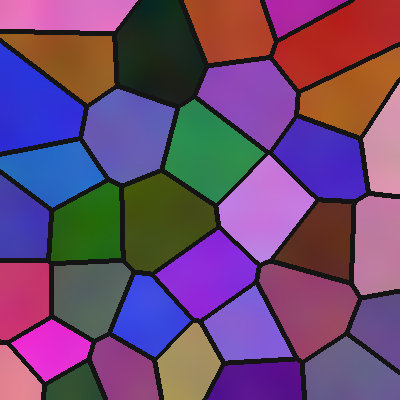
\includegraphics[width=36mm]{assets/drawn/grain-map}};
  \draw[white,line width=0.6pt] (map.south west) rectangle (map.north east);
  \draw[white,line width=0.9pt,-{Stealth[length=2mm,width=1.6mm]}] (131.5,-50.5) -- (131.5,-57);
  % the plane: 36 x 22 mm, yield strength 340-1000 MPa, elongation 30-86 %
  \begin{scope}[shift={(113.5,-83)}]
    \draw[white,line width=0.7pt] (0,22) -- (0,0) -- (36,0);
    \begin{scope}[x=0.054545mm,y=0.392857mm,shift={(-340,-30)}]
      \drawfront[white!75!udsblue,line width=0.6pt,dash pattern=on 1.4pt off 1pt]
      \foreach \s/\e/\i in \alloydata
        \node[circle,fill=white!85!udsblue,inner sep=0pt,minimum size=1.1mm] at (\s,\e) {};
      \node[circle,fill=white,inner sep=0pt,minimum size=4.6mm] (star) at (790,64) {};
      \node[text=udsred,font=\footnotesize] at (star) {\faStar};
    \end{scope}
  \end{scope}
  \fill[udsred] (102,1) rectangle (103.6,-91);}

% \doiline: https://doi.org/ and the paper's DOI, as a link in the slides; in the speaker notes, whose
% thumbnails scale the slide but not its links, the same text without a link
\newcommand\audiencemode{hide notes}
\ifx\notesmode\audiencemode
  \newcommand\doiline{\href{https://doi.org/\paperdoi}{https://doi.org/\paperdoi}}
\else
  \newcommand\doiline{\textcolor{udsblue}{https://doi.org/\paperdoi}}
\fi

% ------------------------------------------------------------------ title
\begin{frame}[plain,noframenumbering]
% Drawn inside the frame rather than over the page, so the speaker notes' thumbnail shows it too.
% The picture's origin is the page's top-left corner: a plain frame's body starts 8 mm in and
% 2 mm down.
\vbox to 0pt{\vskip-2mm\hbox to 0pt{\hskip-8mm\begin{tikzpicture}[x=1mm,y=1mm]
  \useasboundingbox (0,0) rectangle (160,-90);
  \titlepanel
  \node[anchor=north west,inner sep=0pt] at (8,-8) {\includegraphics[width=30mm]{\udslogo}};
  % the text block grows upwards from the presenter's name, whose baseline stays 66.5 mm from the top,
  % at the same distance from the d3M block as in the Coding Agents talk; the citation and the DOI under
  % it form one block, and the red rule sits halfway between that block and the name
  \node[anchor=south west,inner sep=0pt,text width=90mm,align=left,
    execute at begin node={\hyphenpenalty=10000\exhyphenpenalty=10000}] at (8,-66.63) {%
    {\fontsize{16.5}{18}\selectfont\bfseries\color{udsblue}\inserttitle\par}\vskip2mm
    {\fontsize{12}{14.5}\selectfont\color{udsdark}\insertsubtitle\par}\vskip0.6mm
    {\fontsize{9}{11}\selectfont\doiline\par}\vskip1.25mm
    \textcolor{udsred}{\rule{14mm}{0.8pt}}\par\vskip3mm
    {\fontsize{11}{13}\selectfont\color{udsdark}\insertauthor\par}};
  \node[anchor=south west,inner sep=0pt] (d3m) at (8,-83) {
\includegraphics[width=10mm]{assets/d3m.png}};
  \node[anchor=west,inner sep=0pt,text width=74mm,align=left,font=\fontsize{7}{8.8}\selectfont,
    execute at begin node={\hyphenpenalty=10000}] at ([xshift=3mm]d3m.east) {%
    {\color{udsblue}\insertinstitute\par}
    {\color{udsgrey}\insertdate\par}};
\end{tikzpicture}\hss}\vss}
% a frame with no tall content drops out of the notes' thumbnail; this invisible strut keeps it
\par\rule{0pt}{80mm}
\note{\textbf{0:00--0:20}\par
    A paper from Nature Communications, published at the end of September 2026.\par
    The authors train generative models on electron backscatter diffraction (EBSD) maps of 25 variants of
      one alloy, and search them for microstructures that are both stronger and more ductile.\par
    I follow the paper's own story.}
\end{frame}

% ---------------------------------------------------------------- outline
\begin{frame}{Outline}
  % each section's title as on its divider, and the divider's question
  \small\renewcommand\arraystretch{1.4}\setlength\tabcolsep{4pt}
  \begin{tabularx}{\textwidth}{@{}>{\leavevmode\color{udsblue}\bfseries}p{4mm}>{\bfseries}p{42mm}X@{}}
    \toprule
    1 & The design problem   & Why ask a generative model for new microstructures?\\
    2 & Groundwork           & Which methods does the paper build on?\\
    3 & The method           & How are microstructures generated and steered toward properties?\\
    4 & The results          & What do the authors show?\\
    \bottomrule
  \end{tabularx}
  \note{\textbf{0:20--0:50}\par
    Four sections, each answering one question.\par
    Section 2 introduces the machine-learning methods the paper combines, with their origins, for anyone
      who has not followed that literature.\par
    Sections 3 and 4 present the paper as the authors tell it.}
\end{frame}

\section[Problem]{The design problem}
\sectionframe{01}{The design problem}{Why ask a generative model for new microstructures?}{\faBalanceScale}

% ------------------------------------------------------------ the trade-off
\begin{frame}[source={Liao et al.\ (2026), Nat.\ Commun.\ 17, 11232}]{Strength/ductility trade-off}
  \begin{tikzpicture}[x=1mm,y=1mm]
    \useasboundingbox (0,0) rectangle (144,-54);
    \begin{scope}[shift={(16,-42)}]
      \planeaxes{340}{1000}{28}{86}{124}{42}{400,500,...,1000}{30,40,...,80}
      \begin{scope}[plane]
        \drawfront[front]
        \drawalloys
        \draw[udsred,line width=1.1pt,-{Stealth[length=2.6mm,width=2mm]}] (640,55) -- (760,72);
        \node[anchor=west,inner sep=0pt,font=\footnotesize\bfseries,text=udsred] at (768,73.5)
          {goal: stronger and more ductile};
        % the two ends of the trade-off, each beside the axis it is close to
        \node[anchor=west,inner sep=0pt,font=\footnotesize\bfseries,text=udsdark] at (410,84) {ductile, but weak};
        \node[anchor=east,inner sep=0pt,font=\footnotesize\bfseries,text=udsdark] at (1000,41) {strong, but brittle};
        \node[anchor=west,label text] at (360,33) {25 alloys, one processing route each};
        \node[anchor=west,small label] (fl) at (600,40) {measured front};
        \draw[udsgreymid,line width=0.4pt] (fl.north east) -- (700.46,45);
      \end{scope}
    \end{scope}
    \node[axis label] at (78,-49.4) {yield strength (MPa)};
    \node[axis label,rotate=90] at (3,-21) {elongation (\%)};
  \end{tikzpicture}
  \note{\textbf{1:00--2:10}\par
    Each point is one alloy: Inconel 625, a nickel-based superalloy used for turbine discs, blades and
      combustors, processed in one of 25 ways.\par
    The alloys differ only in processing: hot rolling and annealing at different temperatures and
      times.\par
    Each was tensile-tested for its yield strength and its elongation to failure.\par
    The stronger variants stretch less: a strength--ductility trade-off; making a metal stronger
      usually makes it brittle, and making it ductile makes it weak.\par
    The dashed staircase is the front: no measured alloy beats a point on it in both properties.\par
    The goal is a microstructure above and to the right of the front.\par
    Such microstructures are usually found by experience and trial and error over processing
      routes; the paper asks a generative model to propose them.}
\end{frame}

% ------------------------------------------------------- failure case
\begin{frame}[source={Liao et al.\ (2026), Nat.\ Commun.\ 17, 11232, Fig.\ 2c (CC BY-NC-ND 4.0)}]
  {Classic pixelwise loss fails}
  \begin{tikzpicture}[x=1mm,y=1mm]
    \useasboundingbox (0,0) rectangle (144,-54);
    \figpart{32}{0}{2}{340}{770}{1897}{1268}{112}
    \node[anchor=east,label text,align=right] at (29,{\fpy{884}}) {real patches};
    \node[anchor=east,label text,align=right,text=udsred] (pl) at (29,{\fpy{1155}}) {pixel loss only};
    % the two classic pixel losses over the n pixels of a patch x and its reconstruction
    \node[anchor=north east,inner sep=0pt,font=\scriptsize,text=udsdark,align=right] at ([yshift=-1.6mm]pl.south east)
      {MAE $=\frac{1}{n}\sum_i|x_i-\hat{x}_i|$\\[1.2mm] MSE $=\frac{1}{n}\sum_i(x_i-\hat{x}_i)^2$};
    \warnstrip{-41.4}{blurred or missing grain boundaries, colours mixed inside grains}
  \end{tikzpicture}
  \note{\textbf{2:10--3:10}\par
    These are real patches of 50 by 50 micrometres from test alloys, cut from EBSD maps.\par
    In an EBSD map each pixel's colour encodes the crystal orientation there: the three Euler angles
      as red, green and blue; the black lines are grain boundaries.\par
    The second row is what the paper's generator returns when it is trained to reproduce its input
      with a pixel loss alone, the mean absolute difference of the pixel values (MAE); the mean squared
      difference (MSE) is the other classic choice, and both average over all pixels.\par
    The boundaries blur, and colours mix inside grains, although a real grain has nearly one
      orientation.\par
    Boundaries cover few pixels, so an average over all pixels barely notices them; yet boundaries
      and orientations are what set the mechanical properties.}
\end{frame}

% ------------------------------------------------------------- the idea
\begin{frame}[source={Liao et al.\ (2026), Nat.\ Commun.\ 17, 11232, after Figs.\ 1 and 4f}]{Two fixes}
  \begin{tikzpicture}[x=1mm,y=1mm]
    \useasboundingbox (0,0) rectangle (144,-54);
    \tikzset{verdict mark/.style={circle,text=white,inner sep=0pt,minimum size=3.8mm,font=\scriptsize},
      head/.style={anchor=west,inner sep=0pt,font=\footnotesize\bfseries},
      panel title/.style={anchor=north west,inner sep=0pt,font=\footnotesize\bfseries,text=udsdark},
      note/.style={anchor=north west,label text,text width=22mm}}
    % column heads: what goes wrong, and what the paper changes
    \node[verdict mark,fill=udsred] (bad) at (1.9,-1.9) {\faTimes};
    \node[head,text=udsred] at ([xshift=1.6mm]bad.east) {the obstacle};
    \node[verdict mark,fill=testgreen] (good) at (87.9,-1.9) {\faCheck};
    \node[head,text=testgreen] at ([xshift=1.6mm]good.east) {the paper's fix};
    % row 1, the loss: the same patch region, three times enlarged, before and after
    \fill[redtint] (0,-5.6) rectangle (58,-28.4);
    \fill[greentint] (86,-5.6) rectangle (144,-28.4);
    \node[panel title] at (2.4,-7.4) {$L=L_{\mathrm{pix}}$};
    \node[panel title] at (88.4,-7.4) {$L=L_{\mathrm{pix}}+\textcolor{testgreen}{L_{\mathrm{edge}}+L_{\mathrm{SSIM}}}$};
    \foreach \x/\img in {2.4/grain-map-blurred,88.4/grain-map} {
      \node[anchor=north west,inner sep=0pt] at (\x,-12.6) {\includegraphics[width=14mm]{assets/drawn/\img}};
      \draw[udsdark,line width=0.4pt] ({\x+4.9},-17.5) rectangle ++(4.2,-4.2);
      \begin{scope}
        \clip ({\x+24},-19.6) circle (6.3);
        \node[anchor=north west,inner sep=0pt] at ({\x+3},1.4) {\includegraphics[width=42mm]{assets/drawn/\img}};
      \end{scope}
      \draw[udsdark,line width=0.5pt] ({\x+24},-19.6) circle (6.3);
      \draw[udsdark,line width=0.3pt] ({\x+9.1},-17.5) -- ({\x+19.6},-15.1) ({\x+9.1},-21.7) -- ({\x+19.6},-24.1);}
    \node[note] at (121.4,-13.4) {sharp boundaries, one colour per grain};
    \fixarrow{60.4}{83.6}{-17}{more terms}
    % row 2, the sampling: the latent space sampled at random, and searched toward targets (after Fig. 1c)
    \fill[redtint] (0,-31.2) rectangle (58,-54);
    \fill[greentint] (86,-31.2) rectangle (144,-54);
    \node[panel title] at (2.4,-33) {random sampling};
    \node[panel title] at (88.4,-33) {property-guided search};
    \tikzset{code/.style={circle,fill=udsgreymid,inner sep=0pt,minimum size=1.3mm},
      new code/.style={circle,fill=udsblue,inner sep=0pt,minimum size=1.5mm},
      latent/.style={fill=white,draw=udsgreylight,line width=0.4pt}}
    % left: codes drawn at random fall among the training codes
    \filldraw[latent] (14,-43.6) ellipse (10 and 7);
    \foreach \x/\y in {9.6/-38.6,7/-41.4,5.8/-43.8,8.4/-45,9.8/-48.4,14.6/-38.4,19.6/-39,18.6/-48.2,14.8/-49.2}
      \node[code] at (\x,\y) {};
    \node[anchor=north,small label] at (14,-51.2) {latent space};
    % the three new codes join, and one arrow goes on to the sentence about them; the training codes
    % leave each line a clear path
    \node[note,text width=27mm,anchor=west] at (28.4,-43.6) {new codes fall among the training codes};
    \foreach \x/\y in {12/-40.4,15.8/-43.6,11.2/-47}
      \draw[udsblue,line width=0.5pt,shorten <=1mm] (\x,\y) to[out=0,in=180] (22.4,-43.6);
    \draw[udsblue,line width=0.5pt,-{Stealth[length=1.5mm,width=1.1mm]}] (22.4,-43.6) -- (27.4,-43.6);
    \foreach \x/\y in {12/-40.4,15.8/-43.6,11.2/-47} \node[new code] at (\x,\y) {};
    % right: the search steers codes to targets outside them, beyond the measured front (after Fig. 1c)
    \filldraw[latent] (97.6,-45) ellipse (8 and 5.8);
    \foreach \x/\y in {-4.6/1.4,-2/-2.4,0.4/2.6,2.2/-0.6,4.6/1.6,-0.6/-4,5/-2.6,-5.4/-1.2}
      \node[code] at (97.6+\x,-45+\y) {};
    \draw[udsblue,line width=0.9pt,-{Stealth[length=1.8mm,width=1.4mm]}] (104.8,-42.6) -- (107.9,-41.4);
    \filldraw[fill=udsblue!22,draw=udsblue,line width=0.4pt] (111.2,-40.6) circle (3.2);
    \foreach \x/\y in {-1.2/0.9,1.2/-0.9} \node[text=udsred,font=\tiny] at (111.2+\x,-40.6+\y) {\faStar};
    \node[anchor=north,small label] at (97.6,-51.2) {latent space};
    \node[anchor=north,small label] at (111.2,-44.2) {targets};
    \begin{scope}[shift={(119,-49.4)}]
      \draw[udsgreymid,line width=0.5pt] (0,11.4) -- (0,0) -- (22,0);
      \node[anchor=north,small label] at (11,-0.6) {strength};
      \node[anchor=south,small label,rotate=90] at (-0.6,5.7) {elongation};
      \begin{scope}[x=0.033333mm,y=0.203571mm,shift={(-340,-30)}]
        \drawfront[front]
        \drawalloys[minimum size=1mm]
        \draw[udsred,line width=0.7pt,-{Stealth[length=1.6mm,width=1.2mm]}] (600,51) -- (660,61);
        \drawcandidates[minimum size=1.3mm]
      \end{scope}
    \end{scope}
    \fixarrow{60.4}{83.6}{-42.2}{steer by properties}
  \end{tikzpicture}
  \note{\textbf{3:10--4:10}\par
    The paper answers two obstacles with two changes: the obstacles on the left, its fixes on the
      right.\par
    First, a pixel loss alone blurs grain boundaries, as the enlarged region shows; the paper adds two
      terms, one that responds to grain boundaries and one to the structure inside grains.\par
    Second, codes drawn at random from the model's latent space fall among the training codes, so the new
      samples resemble the measured alloys.\par
    So the authors search the latent space, steered by predicted strength and ductility, toward targets
      outside the training codes, as their Fig.~1c sketches; their five candidates lie beyond the measured
      front.\par
    Section 2 explains the models and the search for anyone who has not met them.}
\end{frame}

\section[Groundwork]{Groundwork}
\sectionframe{02}{Groundwork}{Which methods does the paper build on?}{\faBookOpen}

% ----------------------------------------------------- three ways to generate
\begin{frame}[source={Kingma and Welling (2013), arXiv:1312.6114 · Goodfellow et al.\ (2014), NeurIPS · Ramesh et al.\ (2021), ICML · Ho et al.\ (2020), NeurIPS · Rombach et al.\ (2022), CVPR}]
  {Three ways to generate an image}
  \begin{tikzpicture}[x=1mm,y=1mm]
    \useasboundingbox (0,0) rectangle (144,-54);
    \foreach \i/\c/\h in {0/udsblue/In one pass,1/udsgreymid/Token by token,2/udsblue/Step by step from noise} {
      \pgfmathsetmacro\cx{\i*49}
      \fill[\c!8] (\cx,-5.4) rectangle ++(46,-41.6);
      \cardhead{\cx}{0}{46}{\c}{\h}
    }
    % in one pass: a code, decoded into the whole image
    \filldraw[fill=udsblue,draw=udsblue] (6,-12.3) rectangle (10.4,-19.7);
    \node[text=white,font=\small\itshape,inner sep=0pt] at (8.2,-16) {z};
    \draw[flow] (11,-16) -- (14.2,-16);
    \filldraw[fill=bluetint,draw=udsblue,line width=0.5pt] (15,-12.5) -- (25.4,-9) -- (25.4,-23) -- (15,-19.5) -- cycle;
    \node[label text,rotate=90] at (20.2,-16) {decoder};
    \draw[flow] (26,-16) -- (29.2,-16);
    \node[anchor=north west,inner sep=0pt] at (30,-9.5) {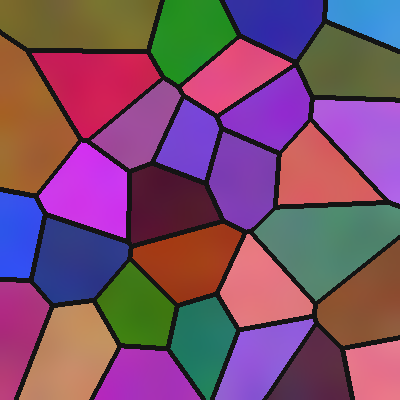
\includegraphics[width=13mm]{assets/drawn/grain-map-new}};
    % token by token: tiles written in reading order, the next one outlined
    \node[anchor=north west,inner sep=0pt] at (65,-9) {
\includegraphics[width=14mm]{assets/drawn/tokens-partial}};
    \begin{scope}[shift={(65,-23)}]
      \draw[udsgreylight,line width=0.3pt] (0,0) grid[step=1.75] (14,14);
      \draw[udsred,line width=0.8pt] (5.25,7) rectangle (7,8.75);
    \end{scope}
    % step by step from noise: the whole image refined at every step
    \foreach \t/\x in {1000/100.5,150/116,0/131.5}
      \node[anchor=north west,inner sep=0pt] at (\x,-10.5) {\includegraphics[width=11mm]{assets/drawn/diffusion-t\t}};
    \draw[flow,draw=udsblue] (112,-16) -- (115.4,-16);
    \draw[flow,draw=udsblue] (127.5,-16) -- (130.9,-16);
    % what each does, examples, and how the image is built
    \foreach \i/\a/\e/\b in {0/{a decoder turns a code into an image}/{VAE (2013), GAN (2014)}/{whole image at once},
        1/{a network predicts each tile from the tiles before it}/{DALL-E 1 (2021); language models write text
          this way}/{no going back to refine},
        2/{a network removes a little noise at each step}/{DDPM (2020), Stable Diffusion (2022), DALL-E 2
          (2022)}/{refines the whole image}} {
      \node[card text,text width=42mm] at ({\i*49+2},-26.6) {\a};
      \node[card text,text width=42mm,font=\scriptsize,text=udsgrey] at ({\i*49+2},-35) {\e};
      \node[card text,text width=42mm,font=\footnotesize\bfseries] at ({\i*49+2},-42.4) {\b};}
    \node[anchor=north west,small label,text=udsred] at (0,-49.4)
      {Liao et al.\ join the first and the third: the VAE output guides the diffusion steps};
  \end{tikzpicture}
  \note{\textbf{4:20--5:20}\par
    Generative models differ in how they build an image.\par
    In one pass: a decoder turns a short code into the whole image at once; VAEs and GANs work this
      way.\par
    Token by token: a network predicts each piece of the image from the pieces before it, as language
      models write text word by word; DALL-E 1 (Ramesh and colleagues, 2021) wrote 32 by 32 such tokens,
      which a discrete VAE then decoded into the image.\par
    Such a model starts from scratch and works in a fixed order, so it cannot go back and refine what it
      has written.\par
    Step by step from noise: a diffusion model starts from noise and refines the whole image at every
      step; Stable Diffusion and DALL-E 2 and 3 work this way, and diffusion leads image generation
      today.\par
    The paper joins the first and the third: a VAE generates in one pass, and its output guides the
      diffusion steps.}
\end{frame}

% ------------------------------------------------------------------ VAE
\begin{frame}[source={Kingma and Welling (2013), arXiv:1312.6114}]{Variational Autoencoder (VAE)}
  \begin{tikzpicture}[x=1mm,y=1mm]
    \useasboundingbox (0,0) rectangle (144,-54);
    \tikzset{part/.style={fill=bluetint,draw=udsblue,line width=0.5pt}}
    % encode, sample, decode; the row's centre line is y = -11.5
    \node[anchor=north west,inner sep=0pt] at (0,-5.5) {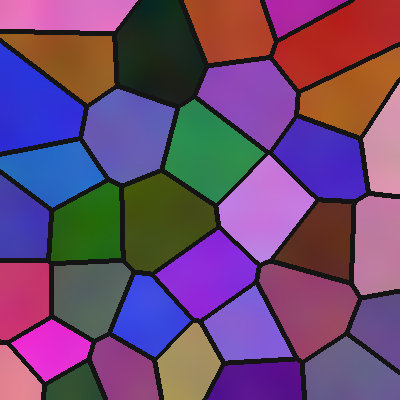
\includegraphics[width=12mm]{assets/drawn/grain-map}};
    \node[anchor=north,small label,text=udsdark] at (6,-18.4) {patch};
    \draw[flow] (12.6,-11.5) -- (16.6,-11.5);
    \filldraw[part] (17.4,-4) -- (27.8,-7.5) -- (27.8,-15.5) -- (17.4,-19) -- cycle;
    \node[label text,rotate=90] at (22.6,-11.5) {encoder};
    \draw[flow] (28.4,-11.5) -- (31.4,-11.5);
    \filldraw[fill=bluetint,draw=udsblue,line width=0.5pt] (32,-6.8) rectangle (36,-11.1);
    \filldraw[fill=darktint,draw=udsdark,line width=0.5pt] (32,-11.9) rectangle (36,-16.2);
    \node[font=\scriptsize,inner sep=0pt,text=udsdark] at (34,-8.95) {$\mu$};
    \node[font=\scriptsize,inner sep=0pt,text=udsdark] at (34,-14.05) {$\sigma$};
    \node[anchor=north,small label,text=udsdark,align=center] at (34,-18.4) {mean,\\ spread};
    \draw[flow] (36.6,-11.5) -- (39.6,-11.5);
    % sample: a normal curve with one drawn value
    \draw[udsgreymid,line width=0.4pt] (40.4,-14.5) -- (49.6,-14.5);
    \draw[udsblue,line width=0.7pt] plot[domain=-2.6:2.6,samples=41] ({45+\x*1.75},{-14.5+6.5*exp(-((\x)^2)/2)});
    \node[circle,fill=udsred,inner sep=0pt,minimum size=1.5mm] at (46.6,-14.5) {};
    \node[anchor=north,small label,text=udsdark] at (45,-18.4) {sample $z$};
    \draw[flow] (50.2,-11.5) -- (53.2,-11.5);
    \filldraw[part] (54,-7.5) -- (64.4,-4) -- (64.4,-19) -- (54,-15.5) -- cycle;
    \node[label text,rotate=90] at (59.2,-11.5) {decoder};
    \draw[flow] (65,-11.5) -- (69,-11.5);
    \node[anchor=north west,inner sep=0pt] at (69.6,-5.5) {
\includegraphics[width=12mm]{assets/drawn/grain-map-blurred}};
    \node[anchor=north,small label,text=udsdark] at (75.6,-18.4) {reconstruction};
    % the loss, each term labelled
    \node[font=\large,text=udsdark,inner sep=0pt] at (4,-32) {$L\;=$};
    \node[font=\large,text=udsdark,inner sep=0pt] (rec) at (21,-32) {$L_{\mathrm{rec}}$};
    \node[font=\large,text=udsdark,inner sep=0pt] at (41,-32) {$+$};
    \node[font=\large,text=udsblue,inner sep=0pt] (kl) at (62,-32) {$L_{\mathrm{KL}}$};
    \node[anchor=north,label text,align=center,text width=28mm] at (21,-36.4) {output close\\ to the input};
    \node[anchor=north,label text,align=center,text width=28mm,text=udsblue] at (62,-36.4)
      {codes close to\\ a standard normal};
    % the latent space: each patch's code is a small cloud, and the clouds overlap
    \draw[udsgreymid,line width=0.5pt] (92,0) rectangle (144,-44);
    \node[anchor=north west,small label] at (93.4,-1.4) {latent space, 2 of 128 directions};
    \foreach \x/\y in {104/-24,110/-18,111/-29,117/-23,103/-33,118/-33,124/-27,109/-38,98/-28}
      {\fill[udsblue,fill opacity=0.14] (\x,\y) circle (4.4); \fill[udsblue] (\x,\y) circle (0.55);}
    \node[text=udsred,font=\footnotesize,inner sep=0pt] (new) at (114.2,-24.4) {\faStar};
    \node[anchor=north west,inner sep=0pt] (np) at (129.4,-9.4) {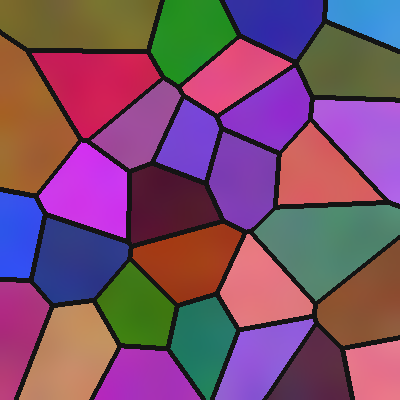
\includegraphics[width=11mm]{assets/drawn/grain-map-new}};
    \draw[udsred,line width=0.7pt,-{Stealth[length=1.6mm,width=1.2mm]}] (new.north east) to[out=40,in=200] (np.west);
    \node[anchor=north,small label,text=udsred,align=center] at (134.9,-21.2) {new code,\\ new patch};
  \end{tikzpicture}
  \note{\textbf{5:20--6:40}\par
    An autoencoder is a network trained to copy its input through a bottleneck: an encoder compresses the
      image into a few numbers, the latent code, and a decoder rebuilds the image from them.\par
    The variational autoencoder, from Kingma and Welling in 2013, makes the code probabilistic: the
      encoder gives a mean and a spread for each number, and the decoder sees a value drawn from that
      range.\par
    A Kullback--Leibler (KL) term pulls every code towards a standard normal distribution, so the codes
      of different images overlap and the space has no gaps.\par
    That makes a VAE generative: a code drawn from this space decodes to a plausible image, and moving
      through the space changes the image smoothly.\par
    Trained with a pixel loss, a VAE returns blurry images, the average of the plausible answers: the
      failure of slide 3.\par
    In this paper each patch gets a code of 128 numbers.}
\end{frame}

% ----------------------------------------------- reconstruct, generate, extrapolate
\begin{frame}{Reconstruct, generate, extrapolate}
  \begin{tikzpicture}[x=1mm,y=1mm]
    \useasboundingbox (0,0) rectangle (144,-54);
    \tikzset{code/.style={circle,fill=udsgreymid,inner sep=0pt,minimum size=1.2mm}}
    \foreach \i/\c/\h in {0/udsdark/Reconstruct,1/udsblue/Generate,2/udsred/Extrapolate} {
      \pgfmathsetmacro\cx{\i*49}
      \fill[\c!8] (\cx,-5.4) rectangle ++(46,-41.6);
      \cardhead{\cx}{0}{46}{\c}{\h}
      % the training codes, the same cloud in every card
      \begin{scope}[shift={(\cx,0)}]
        \filldraw[fill=white,draw=udsgreylight,line width=0.5pt] (21,-16.5) ellipse (8.6 and 5.6);
        \foreach \x/\y in {16/-15,18.6/-19,20.4/-13.6,22.6/-17.4,24.8/-14.6,26.2/-18.4,15.4/-17.8,19.4/-16.2}
          \node[code] at (\x,\y) {};
      \end{scope}
    }
    % reconstruct: a training patch, encoded and decoded
    \node[anchor=north west,inner sep=0pt] (in) at (1.4,-11.5) {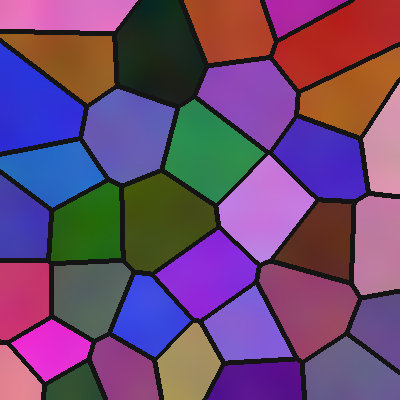
\includegraphics[width=10mm]{assets/drawn/grain-map}};
    \node[circle,draw=udsdark,line width=0.7pt,inner sep=0pt,minimum size=2.6mm] (c0) at (22.6,-17.4) {};
    \draw[flow,line width=0.5pt] (in.east) to[out=0,in=180] (c0.west);
    \node[anchor=north west,inner sep=0pt] (out0) at (34.6,-11.5) {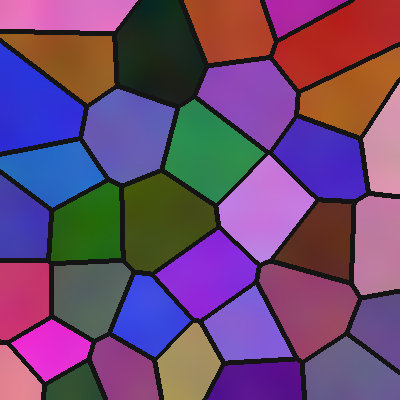
\includegraphics[width=10mm]{assets/drawn/grain-map}};
    \draw[flow,line width=0.5pt] (c0.east) to[out=0,in=180] (out0.west);
    % generate: a new code among the training codes
    \node[circle,fill=udsblue,inner sep=0pt,minimum size=2mm] (c1) at (49+23.4,-15.6) {};
    \node[anchor=north west,inner sep=0pt] (out1) at (49+34.6,-11.5) {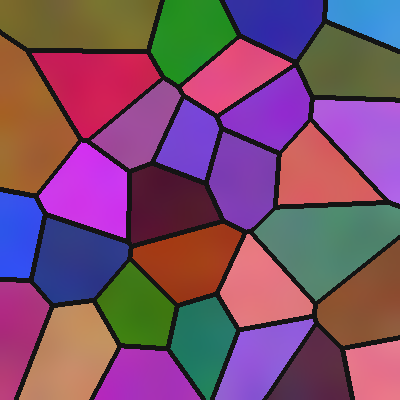
\includegraphics[width=10mm]{assets/drawn/grain-map-new}};
    \draw[flow,draw=udsblue,line width=0.5pt] (c1.east) to[out=0,in=180] (out1.west);
    % extrapolate: a code away from every training code
    \node[text=udsred,font=\footnotesize,inner sep=0pt] (c2) at (98+31.4,-25.4) {\faStar};
    \node[anchor=north west,inner sep=0pt] (out2) at (98+34.6,-11.5) {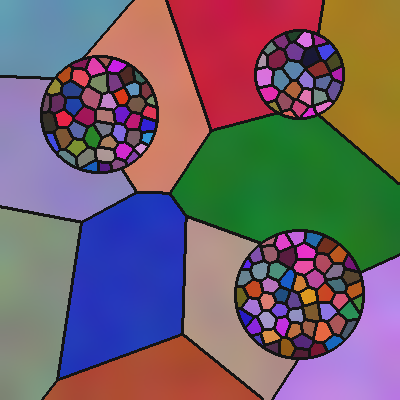
\includegraphics[width=10mm]{assets/drawn/grain-map-bimodal}};
    \node[circle,fill=white,draw=udsred,line width=0.6pt,inner sep=0pt,minimum size=4.2mm,font=\scriptsize\bfseries,
      text=udsred] at ([xshift=-1mm,yshift=1mm]out2.north east) {?};
    \draw[flow,draw=udsred,line width=0.5pt] (c2.east) to[out=0,in=-90] (out2.south);
    % what each is, and what can check it
    \foreach \i/\a/\b in {0/{a training patch, encoded and decoded}/{compare with its input},
        1/{a new code among the training codes}/{compare with held-out data},
        2/{a code away from all training codes}/{only an experiment can tell}} {
      \node[anchor=north west,card text,text width=42mm] at ({\i*49+2},-29.4) {\a};
      \node[anchor=north west,card text,text width=42mm,font=\footnotesize\bfseries] at ({\i*49+2},-41.4) {\b};}
  \end{tikzpicture}
  \note{\textbf{6:40--7:40}\par
    A trained generative model can do three different things, and each needs a different check.\par
    Reconstruct: encode a training patch and decode it again; the result can be compared with its own
      input, pixel by pixel or by its statistics.\par
    Generate: decode a new code from among the training codes; the result has no original, so it is
      compared with the statistics of held-out data and checked for near-copies of training patches.\par
    Extrapolate: decode a code away from all training codes; no example lies there, so only an
      experiment can tell whether the result is realistic.\par
    The paper claims all three; the results show what each claim rests on.}
\end{frame}

% ------------------------------------------------------------ diffusion
\begin{frame}[source={Sohl-Dickstein et al.\ (2015), ICML · Ho et al.\ (2020), NeurIPS · Ronneberger et al.\ (2015), MICCAI}]
  {Diffusion models}
  \begin{tikzpicture}[x=1mm,y=1mm]
    \useasboundingbox (0,0) rectangle (144,-54);
    \node[anchor=north west,label text,text=udsgrey] (fwd) at (0,0)
      {forward: at each of 1000 steps, mix in a little noise\enspace\textcolor{udsgreymid}{(fixed)}};
    \node[anchor=base east,label text] at (fwd.base -| 144,0) {$x_t=\sqrt{1-\beta_t}\,x_{t-1}+\sqrt{\beta_t}\,\epsilon$};
    \foreach \t [count=\i from 0] in {0,50,150,300,1000} {
      \node[anchor=north west,inner sep=0pt] (d\i) at ({2+29*\i},-6.6) {\includegraphics[width=18mm]{assets/drawn/diffusion-t\t}};
      \node[anchor=north,small label,text=udsdark] at ({11+29*\i},-25.4) {$t=\t$};}
    \foreach \i in {0,...,3} {
      \draw[flow,draw=udsgreymid] ({20.6+29*\i},-11.6) -- ({30.4+29*\i},-11.6);
      \draw[flow,draw=udsblue] ({30.4+29*\i},-19.6) -- ({20.6+29*\i},-19.6);}
    \node[anchor=north west,label text,text=udsblue] at (0,-30.4)
      {reverse: a U-Net predicts the noise, removed step by step\enspace\textcolor{udsblue!70}{(learned)}};
    % generating with the trained model, two ways: from noise alone, or from noise and a guide (the paper)
    \tikzset{step image/.style={anchor=west,inner sep=0pt},
      way name/.style={anchor=west,inner sep=0pt,font=\footnotesize\bfseries,text=udsdark},
      way text/.style={card text,anchor=west,text width=84mm}}
    \node[anchor=north west,label text,text=udsgrey] at (0,-34.4) {generating with the trained model, two ways:};
    \foreach \y in {-41.6,-49.8} \fill[bluetint] (0,\y+3.9) rectangle (144,\y-3.9);
    % unconditional: noise alone
    \node[way name] at (2.4,-41.6) {unconditional};
    \node[step image] (u0) at (27,-41.6) {
\includegraphics[width=6.6mm]{assets/drawn/diffusion-t1000}};
    \node[step image] (u1) at (49.4,-41.6) {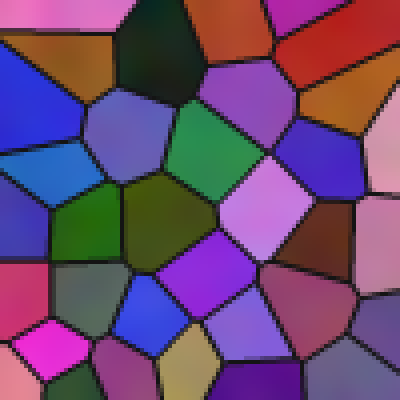
\includegraphics[width=6.6mm]{assets/drawn/diffusion-t0}};
    \draw[flow,draw=udsblue] ([xshift=0.6mm]u0.east) -- ([xshift=-0.6mm]u1.west);
    \node[way text] at (59,-41.6) {from noise alone, step by step: a new patch of any kind};
    % conditional: noise and a guide image
    \node[way name] at (2.4,-49.8) {conditional};
    \node[step image] (c0) at (27,-49.8) {
\includegraphics[width=6.6mm]{assets/drawn/diffusion-t1000}};
    \node[font=\small\bfseries,text=udsdark,inner sep=0pt] at (35.4,-49.8) {+};
    \node[step image] (c1) at (37.2,-49.8) {
\includegraphics[width=6.6mm]{assets/drawn/grain-map-blurred}};
    \draw[udsred,line width=0.6pt] (c1.south west) rectangle (c1.north east);
    \node[step image] (c2) at (49.4,-49.8) {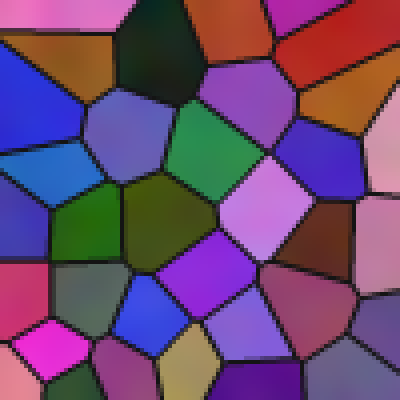
\includegraphics[width=6.6mm]{assets/drawn/diffusion-t0}};
    \draw[flow,draw=udsblue] ([xshift=0.6mm]c1.east) -- ([xshift=-0.6mm]c2.west);
    \node[way text] at (59,-49.8) {the U-Net also sees a \textcolor{udsred}{guide} at every step, here the VAE
      output};
  \end{tikzpicture}
  \note{\textbf{7:40--8:50}\par
    A diffusion model learns to undo noise.\par
    The forward process is fixed: each of 1000 steps scales the image down slightly and adds a little
      Gaussian noise $\epsilon$, with $\beta_t$ rising from 0.0001 to 0.02; after a few hundred steps only
      noise is left.\par
    Each step depends only on the one before, a Markov chain; the paper writes it as a Gaussian, its
      Eq.~12.\par
    The reverse process is learned: a network predicts the noise in an image at any step, and removing it
      step by step runs the process backwards.\par
    The idea is from Sohl-Dickstein and colleagues, 2015; DDPM, from Ho, Jain and Abbeel in 2020, made
      the images sharp.\par
    Once trained, it generates in two ways: from noise alone, any new patch; or with a guide image that
      the U-Net sees at every step, a patch that follows the guide.\par
    The paper's guide is the VAE's blurry output, so the diffusion model only restores detail; the next
      slide shows the training.}
\end{frame}

% ---------------------------------------------------- training a diffusion model
\begin{frame}[source={Ho et al.\ (2020), NeurIPS · Ronneberger et al.\ (2015), MICCAI}]
  {Training a diffusion model}
  \begin{tikzpicture}[x=1mm,y=1mm]
    \useasboundingbox (0,0) rectangle (144,-54);
    \begin{scope}[yshift=1mm]% content starts 4 mm below the title
    % a patch and a noise image, mixed in one go to a random step t
    \node[anchor=north west,inner sep=0pt] (x0) at (0,-1) {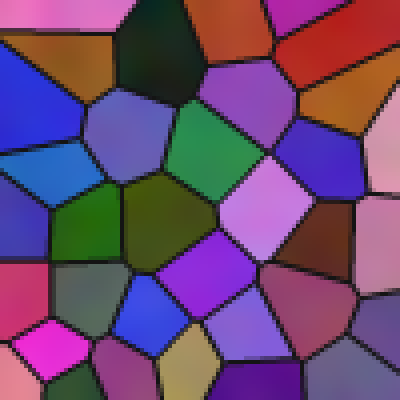
\includegraphics[width=12mm]{assets/drawn/diffusion-t0}};
    \node[anchor=north,small label,text=udsdark] at (6,-13.8) {patch $x_0$};
    \node[anchor=north west,inner sep=0pt] (eps) at (0,-21) {
\includegraphics[width=12mm]{assets/drawn/diffusion-noise}};
    \node[anchor=north,small label,text=udsdark] at (6,-33.8) {noise $\epsilon$};
    \node[draw=udsgreymid,fill=darktint,line width=0.5pt,inner sep=1.6mm,align=center,font=\footnotesize,
      text=udsdark] (mix) at (39,-7)
      {{\scriptsize\color{udsgrey}a random step $t$, in one go}\\[0.6mm]
       $x_t=\sqrt{\bar\alpha_t}\,x_0+\sqrt{1-\bar\alpha_t}\,\epsilon$};
    \draw[flow] (x0.east) -- (x0.east -| mix.west);
    \draw[flow] (12,-24) to[out=0,in=-90] (30,-12.6 |- mix.south);
    % the noised patch and its step go into the U-Net, which predicts the noise
    \node[anchor=north west,inner sep=0pt] (xt) at (66,-1) {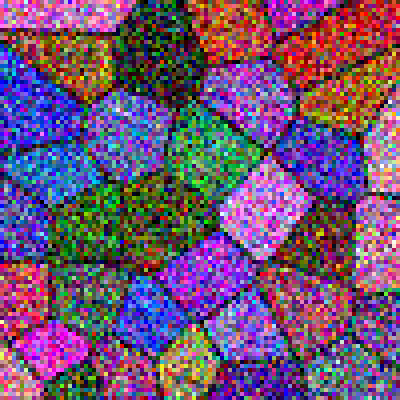
\includegraphics[width=12mm]{assets/drawn/diffusion-t150}};
    \node[anchor=north,small label,text=udsdark] at (72,-13.8) {$x_t$, here $t=150$};
    \draw[flow] (mix.east) -- (mix.east -| xt.west);
    \node[draw=udsblue,fill=bluetint,line width=0.5pt,minimum width=14mm,minimum height=9mm,font=\footnotesize,
      text=udsblue,inner sep=0pt] (unet) at (92,-7) {U-Net};
    \draw[flow] (xt.east |- unet.west) -- (unet.west);
    \node[anchor=north,small label,text=udsdark] (tin) at (92,-17.4) {step $t$};
    \draw[flow,line width=0.5pt] (tin.north) -- (unet.south);
    \node[anchor=west,font=\footnotesize,text=udsblue,inner sep=0pt] (pred) at (105.2,-7) {$\epsilon_\theta(x_t,t)$};
    \node[anchor=north,small label,text=udsblue] at ([yshift=-1.4mm]pred.south) {predicted noise};
    \draw[flow] (unet.east) -- (pred.west);
    % the loss: the predicted noise against the noise that was added
    \node[draw=udsred,fill=redtint,line width=0.5pt,inner sep=1.6mm,font=\footnotesize,text=udsdark] (loss)
      at (pred.center |- 0,-29) {$\|\epsilon-\epsilon_\theta(x_t,t)\|^2$};
    \draw[flow] ([yshift=-5.6mm]pred.south) -- (loss.north);
    \draw[flow,draw=udsred] (eps.east |- loss.west) -- (loss.west);
    \node[anchor=south,small label,text=udsred] at (56,-28.4) {the noise that was added is the target};
    \node[anchor=west,small label,text width=14mm] at ([xshift=1.6mm]loss.east) {loss: trains the U-Net};
    \end{scope}
    % repeated over many patches; the paper adds the VAE output as an input
    \fill[bluetint] (0,-40.4) rectangle (70,-53.6);
    \node[card text,anchor=west,text width=66mm] at (2,-47) {repeated over many patches, steps and noise
      images: one U-Net learns all 1000 steps};
    \fill[redtint] (74,-40.4) rectangle (144,-53.6);
    \node[card text,anchor=west,text width=66mm] at (76,-47) {Liao et al.: the U-Net also sees the VAE output,
      $\epsilon_\theta(x_t,t,x_V)$};
  \end{tikzpicture}
  \note{\textbf{8:50--10:00}\par
    A diffusion model is trained on one simple task: predict the noise in a noised image.\par
    Take a training patch $x_0$, draw a noise image $\epsilon$ and a random step $t$, and mix them in one
      go; $\bar\alpha_t$, the product of all $1-\beta_s$ up to step $t$, says how much of the patch is
      left.\par
    The network, a U-Net (Ronneberger and colleagues, 2015), gets the noised patch and the step and returns
      a noise image of the same size.\par
    The loss is the squared error between the added and the predicted noise; repeated over many patches,
      steps and noise images, one network learns every step.\par
    Knowing the noise is enough to step back: each reverse step subtracts a share of the predicted noise
      and adds a little fresh noise.\par
    The paper trains its diffusion model this way, with the VAE output $x_V$ as a third input, and
      compares the noise with the loss of section 3.}
\end{frame}

% --------------------------------------------------------- Pareto, NSGA-II
\begin{frame}[source={Pareto (1906), \emph{Manuale di economia politica} · Holland (1975), \emph{Adaptation in Natural and Artificial Systems} · Deb et al.\ (2002), IEEE Trans.\ Evol.\ Comput.\ 6, 182}]
  {Pareto fronts and NSGA-II}
  \begin{tikzpicture}[x=1mm,y=1mm]
    \useasboundingbox (0,0) rectangle (144,-54);
    \tikzset{panel frame/.style={draw=udsgreylight,line width=0.5pt,rounded corners=1mm},
      name part/.style={anchor=north,inner sep=0pt,font=\Large\bfseries,text=udsblue},
      name meaning/.style={anchor=north,small label,text=udsdark},
      front point/.style={circle,fill=udsblue,inner sep=0pt,minimum size=1.6mm},
      back point/.style={circle,fill=udsgreymid,inner sep=0pt,minimum size=1.6mm},
      point name/.style={inner sep=0pt,font=\scriptsize\bfseries,text=udsdark},
      ga row/.style={anchor=west,label text},
      ga icon/.style={font=\footnotesize,text=udsblue}}
    % the name, part by part, over the panel that explains each part
    \foreach \x/\l/\m in {22/NS/non-dominated sorting,72/GA/genetic algorithm,122/II/crowding distance} {
      \node[name part] at (\x,0) {\l};
      \node[name meaning] at (\x,-5.2) {\m};}
    \foreach \x in {0,50,100} \draw[panel frame] (\x,-9.2) rectangle ++(44,-38.4);
    % NS: A beats B in both goals; nobody beats A, C or D in both, so they form front 1
    \begin{scope}[shift={(5,-43.6)}]
      \draw[udsgreymid,line width=0.5pt,-{Stealth[length=1.4mm,width=1mm]}] (0,0) -- (38,0);
      \draw[udsgreymid,line width=0.5pt,-{Stealth[length=1.4mm,width=1mm]}] (0,0) -- (0,30.4);
      \node[anchor=north east,small label] at (38,-0.6) {goal 1};
      \node[anchor=south east,small label,rotate=90] at (-0.6,30.4) {goal 2};
      \begin{scope}[x=36mm,y=29mm]
        \fill[redtint] (0,0) rectangle (0.8,0.8);
        \node[anchor=south west,small label,text=udsred] at (0.04,0.05) {A beats B in both};
        \draw[udsgreymid,line width=0.6pt,dash pattern=on 1.4pt off 1pt]
          (0.35,0.75) -- (0.35,0.6) -- (0.6,0.6) -- (0.6,0.4) -- (0.7,0.4);
        \draw[udsblue,line width=0.8pt] (0.5,0.95) -- (0.5,0.8) -- (0.8,0.8) -- (0.8,0.5) -- (0.95,0.5);
        \foreach \u/\v in {0.5/0.95,0.8/0.8,0.95/0.5} \node[front point] at (\u,\v) {};
        \foreach \u/\v in {0.35/0.75,0.6/0.6,0.7/0.4} \node[back point] at (\u,\v) {};
        \foreach \n/\u/\v/\dx/\dy/\a in {A/0.8/0.8/0.9/0.9/south west,B/0.6/0.6/0.9/0.9/south west,
            C/0.95/0.5/0/1.2/south,D/0.5/0.95/-1.2/0/east}
          \node[point name,anchor=\a] at ([shift={(\dx mm,\dy mm)}]\u,\v) {\n};
        \node[anchor=west,small label,text=udsblue] at (0.56,0.97) {front 1};
        \node[anchor=north west,small label,text=udsgreymid] at (0.36,0.57) {front 2};
      \end{scope}
    \end{scope}
    % GA: one generation, top to bottom, and round again
    \foreach \y/\icon/\t in {-14.4/\faUsers/population,-22.4/\faBalanceScale/score both goals,
        -30.4/\faFilter/{keep the best: by front,\\ then by crowding},-38.4/\faRandom/{cross over, mutate}} {
      \node[ga icon] at (57.6,\y) {\icon};
      \node[ga row] at (62.4,\y) {\t};}
    \foreach \y in {-14.4,-22.4,-30.4} \draw[flow,draw=udsblue,line width=0.5pt] (57.6,\y-2.4) -- (57.6,\y-5.6);
    \draw[flow,draw=udsblue,line width=0.5pt] (55,-38.4) -- (52.6,-38.4) -- (52.6,-14.4) -- (55,-14.4);
    \node[anchor=north,small label,text=udsdark] at (71.5,-42.2) {repeat for hundreds of generations};
    % the two rules of "keep the best" come from the panels beside it
    \draw[flow,draw=udsblue] (44.6,-30.4) -- (49.4,-30.4);
    \draw[flow,draw=udsblue] (99.4,-30.4) -- (94.6,-30.4);
    % II: on a crowded front, near-copies are dropped and points with room around them kept
    \begin{scope}[shift={(105,-43.6)}]
      \draw[udsgreymid,line width=0.5pt,-{Stealth[length=1.4mm,width=1mm]}] (0,0) -- (38,0);
      \draw[udsgreymid,line width=0.5pt,-{Stealth[length=1.4mm,width=1mm]}] (0,0) -- (0,30.4);
      \node[anchor=north east,small label] at (38,-0.6) {goal 1};
      \node[anchor=south east,small label,rotate=90] at (-0.6,30.4) {goal 2};
      \begin{scope}[x=36mm,y=29mm]
        \draw[testgreen,line width=0.6pt,dash pattern=on 1.2pt off 0.8pt] (0.12,0.62) rectangle (0.76,0.95);
        \draw[udsblue,line width=0.8pt] (0.12,0.95) -- (0.12,0.85) -- (0.45,0.85) -- (0.45,0.62) -- (0.76,0.62)
          -- (0.76,0.6) -- (0.8,0.6) -- (0.8,0.58) -- (0.84,0.58) -- (0.84,0.3) -- (0.95,0.3);
        \foreach \u/\v in {0.12/0.95,0.45/0.85,0.76/0.62,0.8/0.6,0.84/0.58,0.95/0.3} \node[front point] at (\u,\v) {};
        \node[text=udsred,font=\footnotesize\bfseries,inner sep=0pt] at (0.8,0.6) {\faTimes};
        \node[anchor=south west,small label,text=testgreen] at (0.17,0.965) {room around it: kept};
        \node[anchor=north east,small label,text=udsred,align=right] at (0.81,0.53) {near-copy:\\ dropped};
      \end{scope}
    \end{scope}
  \end{tikzpicture}
  \note{\textbf{10:00--11:20}\par
    With two goals that fight each other, such as strength and ductility, there is rarely one best
      answer, only a menu of trade-offs.\par
    NSGA-II, from Deb and colleagues in 2002, searches for that menu, and its name says how.\par
    GA, a genetic algorithm (Holland, 1975): a population of candidates evolves over generations; each is
      scored on both goals, the best become parents, and children mix their parents' parts (crossover)
      with small random changes (mutation).\par
    NS, non-dominated sorting: A beats B because it is better in both goals; nobody beats A, C or D in
      both, so they form front 1, the Pareto front, after Vilfredo Pareto, 1906; without front 1, the
      unbeaten rest form front 2, and the best are taken front by front.\par
    II, crowding distance: when a front has more candidates than places, near-copies are dropped and
      candidates with room around them are kept, so the population spreads along the whole front.\par
    Section 3 shows how the paper runs this search.}
\end{frame}

\section[Method]{The method}
\sectionframe{03}{The method}{How are microstructures generated and steered toward properties?}{\faProjectDiagram}

% ------------------------------------------------------------------ data
\begin{frame}[source={Liao et al.\ (2026), Nat.\ Commun.\ 17, 11232, Methods}]{25 alloys, one map each}
  \begin{tikzpicture}[x=1mm,y=1mm]
    \useasboundingbox (0,0) rectangle (144,-54);
    % the orthogonal design: hot-rolling reduction across, annealing temperature down; each cell one alloy
    \node[anchor=south,label text] at (52,-2.4) {hot-rolling reduction at 900\,°C};
    \foreach \r [count=\c from 0] in {0,20,30,40,50}
      \node[anchor=south,small label,text=udsdark] at ({28+12*\c+6},-7.6) {\r\,\%};
    \foreach \t [count=\c from 0] in {650,750,850,950,1050}
      \node[anchor=east,small label,text=udsdark] at (27,{-8-7*\c-3.5}) {\t\,°C};
    \node[label text,rotate=90] at (5,-25.5) {annealing temperature};
    \foreach \r/\t/\h/\s/\sh in \alloygrid {
      \pgfmathtruncatemacro\c{\r==0 ? 0 : \r/10-1}
      \pgfmathtruncatemacro\w{(\t-650)/100}
      \fill[udsblue!\sh] ({28+12*\c},{-8-7*\w}) rectangle ++(12,-7);
      \ifnum\sh>40\def\tc{white}\else\def\tc{udsdark}\fi
      \node[font=\scriptsize,text=\tc,inner sep=0pt] at ({28+12*\c+6},{-8-7*\w-3.5}) {\h\,h};
    }
    \draw[white,line width=0.6pt] \foreach \c in {1,...,4} {({28+12*\c},-8) -- ++(0,-35)}
      \foreach \w in {1,...,4} {(28,{-8-7*\w}) -- ++(60,0)};
    \node[anchor=north west,small label,text width=62mm] at (28,-45.4)
      {each cell one alloy: its annealing time; darker: higher yield strength};
    % one alloy's data
    \fill[darktint] (96,-5.4) rectangle (144,-52);
    \cardhead{96}{0}{48}{udsdark}{Each alloy}
    \node[anchor=north west,inner sep=0pt] (map) at (98.5,-8)
      {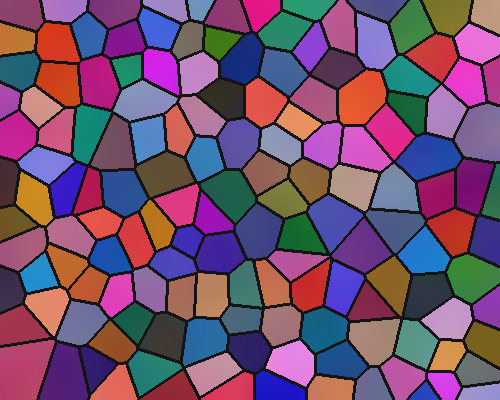
\includegraphics[width=20mm]{assets/drawn/grain-map-wide}};
    \node[anchor=north west,label text,text width=22mm] at (121,-8.4) {EBSD map\\ 1000\,×\,800 px\\ 0.5\,µm per px};
    \node[anchor=north west,label text,text width=42mm] at (98.5,-26.6)
      {colour: $(\varphi_1,\Phi,\varphi_2)\to$ red, green, blue};
    \begin{scope}[shift={(99.5,-48.5)}]
      \draw[udsgreymid,line width=0.5pt] (0,13) -- (0,0) -- (18,0);
      \draw[udsdark,line width=0.9pt] (0,0) -- (1.6,8.2) .. controls (4,10.2) and (12,11.6) .. (15.4,11.2)
        -- (16,8.8);
      \node[circle,fill=udsred,inner sep=0pt,minimum size=1.5mm] at (1.6,8.2) {};
      \node[circle,fill=udsred,inner sep=0pt,minimum size=1.5mm] at (16,8.8) {};
    \end{scope}
    \node[anchor=north west,label text,text width=22mm] at (121,-36.6) {tensile test:\\ yield strength,\\ elongation};
  \end{tikzpicture}
  \note{\textbf{11:30--12:40}\par
    The 25 alloys come from an orthogonal design: five hot-rolling reductions, five annealing
      temperatures and five annealing times, combined so that every pair of levels occurs once.\par
    Each cell is one alloy; the number is its annealing time and the shade its yield strength.\par
    More rolling and lower annealing temperatures give the stronger alloys.\par
    Each alloy has one EBSD map of 1000 by 800 pixels at 0.5 µm per pixel, a field of 500 by 400 µm,
      with the three Euler angles of each pixel stored as red, green and blue.\par
    Each alloy also has one yield strength and one elongation; how many tensile tests stand behind them
      is not stated.\par
    So the dataset is 25 maps and 25 pairs of property values.}
\end{frame}

% ----------------------------------------------------------------- split
\begin{frame}[source={Liao et al.\ (2026), Nat.\ Commun.\ 17, 11232, Results and Methods}]{Alloy split before cropping}
  \begin{tikzpicture}[x=1mm,y=1mm]
    \useasboundingbox (0,0) rectangle (144,-54);
    % stages, left to right
    \foreach \x/\t in {32/{EBSD maps},64/{patches, 100\,×\,100\,px},97/{+ flips, rotations},
        128/{+ degraded copies}}
      \node[anchor=north,label text,align=center] at (\x,0) {\t};
    \node[anchor=north,inner sep=0pt] (m1) at (32,-5.2) {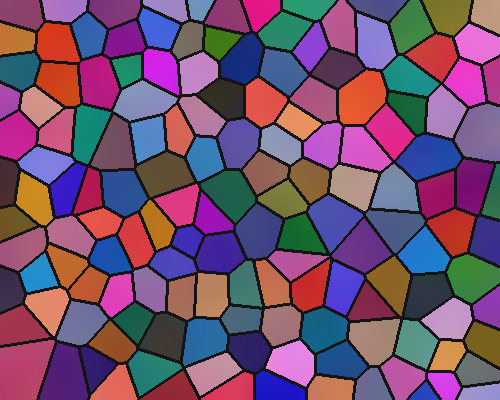
\includegraphics[width=16mm]{assets/drawn/grain-map-wide}};
    \node[anchor=north,inner sep=0pt] (m2) at (64,-5.2) {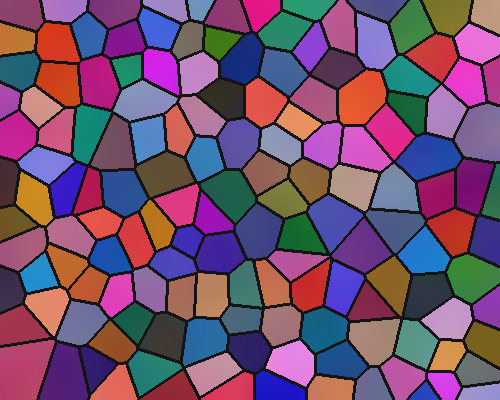
\includegraphics[width=16mm]{assets/drawn/grain-map-wide}};
    \draw[white,line width=0.35pt] \foreach \i in {1,...,9} {([xshift=\i*1.6mm]m2.north west) -- ([xshift=\i*1.6mm]m2.south west)}
      \foreach \j in {1,...,7} {([yshift=-\j*1.6mm]m2.north west) -- ([yshift=-\j*1.6mm]m2.north east)};
    \draw[udsred,line width=0.7pt] (m2.north west) rectangle ([xshift=1.6mm,yshift=-1.6mm]m2.north west);
    \node[inner sep=0pt] at (91.5,-9.7) {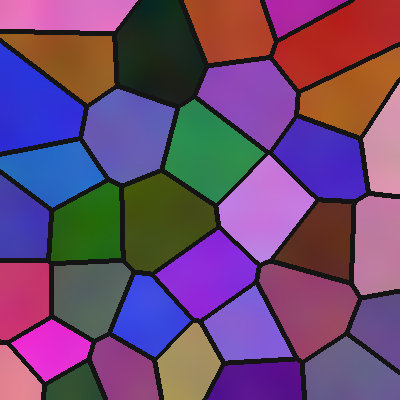
\includegraphics[width=9mm]{assets/drawn/grain-map}};
    \node[inner sep=0pt,rotate=90] at (102.5,-9.7) {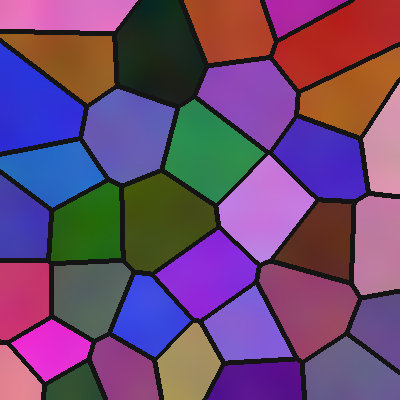
\includegraphics[width=9mm]{assets/drawn/grain-map}};
    \node[inner sep=0pt] at (122.5,-9.7) {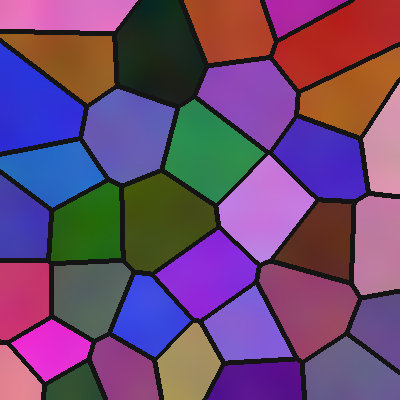
\includegraphics[width=9mm]{assets/drawn/grain-map}};
    \node[inner sep=0pt] at (133.5,-9.7) {
\includegraphics[width=9mm]{assets/drawn/grain-map-blurred}};
    % the two lanes
    \fill[bluetint] (0,-24) rectangle (144,-33.6);
    \fill[redtint] (0,-35.6) rectangle (144,-45.2);
    \node[anchor=west,label text,font=\footnotesize\bfseries,text=udsblue] at (1.6,-28.8) {training};
    \node[anchor=west,label text,font=\footnotesize\bfseries,text=udsred] at (1.6,-40.4) {test};
    \foreach \x/\ta/\tb in {32/{20 alloys}/{5 alloys},64/{1,600}/{400},97/{9,600}/{2,400},128/{57,600}/{14,400}} {
      \node[font=\small\bfseries,text=udsdark,inner sep=0pt] at (\x,-28.8) {\ta};
      \node[font=\small\bfseries,text=udsdark,inner sep=0pt] at (\x,-40.4) {\tb};}
    \foreach \x/\m in {48/\times 80,80.5/\times 6,112.5/\times 6} {
      \draw[flow,draw=udsgreymid] (\x-5,-28.8) -- (\x+5,-28.8);
      \draw[flow,draw=udsgreymid] (\x-5,-40.4) -- (\x+5,-40.4);
      \node[small label,anchor=south] at (\x,-23.4) {$\m$};}
    \goodstrip{-48.4}{test patches come from five alloys the model never sees in training}
  \end{tikzpicture}
  \note{\textbf{12:40--13:30}\par
    The split comes first: the 25 maps are divided at random into 20 training and 5 test alloys.\par
    Only then is each map cut into 80 patches of 100 by 100 pixels, 50 by 50 µm.\par
    Flips and rotations make six versions of each patch.\par
    Each version also gets five degraded copies (blur, distortion, black blocks, erosion and dilation),
      which the model learns to restore.\par
    That gives 72,000 images: 57,600 for training and 14,400 for testing.\par
    Because the split is by alloy, no test patch shares a map with a training patch: the same rule as
      splitting by specimen in segmentation.\par
    The images multiply; the alloys stay 25.}
\end{frame}

% ------------------------------------------------------------- generator
\begin{frame}[source={Liao et al.\ (2026), Nat.\ Commun.\ 17, 11232, Fig.\ 1a (CC BY-NC-ND 4.0) · Pandey et al.\ (2022), Trans.\ Mach.\ Learn.\ Res.}]
  {A VAE, refined by diffusion}
  \begin{tikzpicture}[x=1mm,y=1mm]
    \useasboundingbox (0,0) rectangle (144,-54);
    % Fig. 1a as published: its schematic, without the loss equation below it (pixel rows 0 to 258)
    \figpart{0}{0}{1}{0}{0}{2000}{258}{144}
    % the size of each part, under it; x from the part's pixel columns in the figure
    \tikzset{size/.style={anchor=north,small label,text=udsdark,align=center}}
    \node[size] at ({\fpx{113}},-19.8) {$100\times100$ px};
    \node[size,text=udsred] at ({\fpx{521}},-19.8) {128 numbers};
    \node[size] at ({\fpx{918}},-19.8) {$100\times100$ px};
    \node[size] at ({\fpx{1455}},-19.8) {one U-Net for every step};
    \node[size,anchor=north east] at (144,-19.8) {$100\times100$ px};
    % the two models, each under a bracket
    \draw[udsblue,line width=0.6pt] ({\fpx{40}},-23.6) -- ++(0,-1.4) -| ({\fpx{990}},-23.6);
    \node[anchor=north,label text,align=center,text width=68mm] at ({\fpx{515}},-26.4)
      {\textbf{variational autoencoder (VAE)}\\ three convolutional layers in, three transposed out\\
       loss $L_{\mathrm{pix}}+L_{\mathrm{edge}}+L_{\mathrm{SSIM}}+L_{\mathrm{KL}}$};
    \draw[udsblue,line width=0.6pt] ({\fpx{1148}},-23.6) -- ++(0,-1.4) -| ({\fpx{1997}},-23.6);
    \node[anchor=north,label text,align=center,text width=60mm] at ({\fpx{1572}},-26.4)
      {\textbf{conditional diffusion model (DDPM)}\\ a U-Net predicts the noise, guided by $x_V$\\
       loss: the same three terms on the noise};
    % how the generator is trained, and how it generates
    \foreach \i/\c/\icon/\h/\b in {
        0/udsblue/\faImages/training data/{57,600 images of the 20 training alloys: patches to reproduce,
          and degraded copies to restore},
        1/udsred/\faStar/generation/{a code from the search goes through the decoder, then the diffusion
          model: a new patch}} {
      \fill[\c!8] ({\i*74},-39) rectangle ++(70,-14.6);
      \fill[\c] ({\i*74},-39) rectangle ++(1.2,-14.6);
      \node[anchor=north west,inner sep=0pt,font=\scriptsize\bfseries,text=\c] at ({\i*74+3.4},-40.8)
        {\icon\enspace\h};
      \node[anchor=north west,inner sep=0pt,font=\scriptsize,text=udsdark,text width=64.6mm,align=left,
        execute at begin node={\hyphenpenalty=10000\raggedright}] at ({\i*74+3.4},-44.8) {\b};}
  \end{tikzpicture}
  \note{\textbf{13:30--14:20}\par
    This is the paper's own diagram of its generator, Fig.~1a.\par
    The VAE compresses each patch of 100 by 100 pixels into a code z of 128 numbers and decodes it into
      $x_V$, which is smooth.\par
    A conditional diffusion model then refines $x_V$: its U-Net predicts the noise step by step and sees
      $x_V$ at every step, the pairing of DiffuseVAE; the red arrow marks that condition.\par
    Both models are trained with the pixel, edge and SSIM terms of the next slide: the VAE on its output,
      the diffusion model on the noise it predicts.\par
    Training uses the 57,600 images of the 20 training alloys, with Adam over 100 epochs.\par
    The code z is what the search moves around later.}
\end{frame}

% ------------------------------------------------------------------ loss
\begin{frame}[source={Liao et al.\ (2026), Nat.\ Commun.\ 17, 11232, Eqs.\ 1--9 · Sobel and Feldman (1968), Stanford AI Project · Wang et al.\ (2004), IEEE Trans.\ Image Process.\ 13, 600}]{Optimization Loss}
  \begin{tikzpicture}[x=1mm,y=1mm]
    \useasboundingbox (0,0) rectangle (144,-54);
    % the equation, each term above its column
    \foreach \x/\t in {5/{L\;=},22/{L_{\mathrm{pix}}},47/{+},72/{\color{udsblue}L_{\mathrm{edge}}},97/{+},
        122/{\color{udsblue}L_{\mathrm{SSIM}}}}
      \node[font=\LARGE,text=udsdark,inner sep=0pt] at (\x,-3.2) {$\t$};
    \foreach \x/\c/\h in {0/udsgreymid/{pixel values},50/udsblue/{edges},100/udsblue/{structure}} {
      \fill[\c!8] (\x,-16.6) rectangle ++(44,-35.4);
      \cardhead{\x}{-11.2}{44}{\c}{\h}}
    % pixel values
    \node[anchor=north,font=\small,text=udsdark,inner sep=0pt] at (22,-19.6)
      {$\displaystyle\frac{1}{n}\sum_{i=1}^{n}|x_i-\hat{x}_i|$};
    \node[anchor=north west,card text,text width=40mm] at (2,-31)
      {Mean Absolute\\ Difference (MAE)\\[0.8mm] every pixel weighs the same; boundaries are few pixels};
    % edges
    \node[anchor=north,font=\small,text=udsdark,inner sep=0pt] at (72,-19.6)
      {$\mathrm{mean}\,|S\ast x-S\ast\hat{x}|$};
    \node[anchor=north west,inner sep=0pt] (e1) at (54,-25.4) {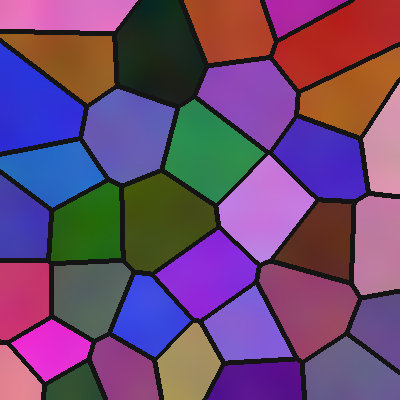
\includegraphics[width=12mm]{assets/drawn/grain-map}};
    \node[anchor=north west,inner sep=0pt] (e2) at (78,-25.4) {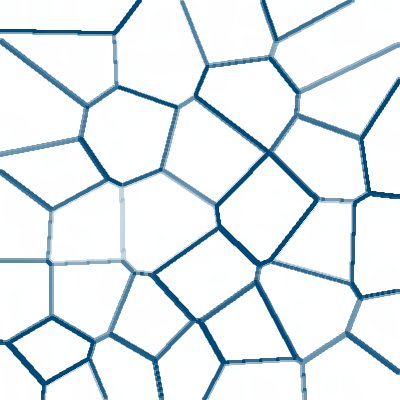
\includegraphics[width=12mm]{assets/drawn/grain-map-edges}};
    \draw[icon frame,udsgreylight] (e2.south west) rectangle (e2.north east);
    \draw[flow,draw=udsblue] (e1.east) -- node[above=0.6mm,small label,text=udsblue] {$S\ast$} (e2.west);
    \node[anchor=north west,card text,text width=40mm] at (52,-40)
      {Sobel filter $S$, across and down: large at grain boundaries};
    % structure
    \node[anchor=north,font=\small,text=udsdark,inner sep=0pt] at (122,-19.6)
      {$1-\mathrm{SSIM}(x,\hat{x})$};
    \node[anchor=north west,inner sep=0pt] (s1) at (104,-25.4) {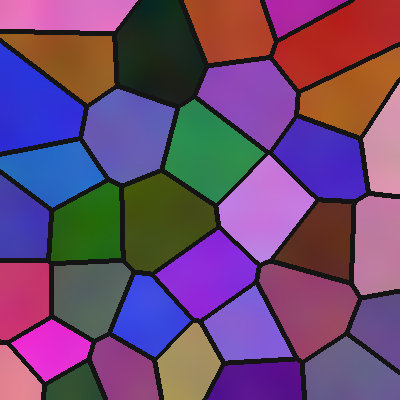
\includegraphics[width=12mm]{assets/drawn/grain-map}};
    \node[anchor=north west,inner sep=0pt] (s2) at (128,-25.4) {
\includegraphics[width=12mm]{assets/drawn/grain-map-blurred}};
    \node[small label,text=udsblue] at (122,-31.4) {$x$ vs $\hat{x}$};
    \node[anchor=north west,card text,text width=40mm] at (102,-40)
      {means, contrasts and correlation: orientation inside grains};
  \end{tikzpicture}
  \note{\textbf{14:20--15:30}\par
    The loss is the sum of three terms, added without weights.\par
    The pixel term is the mean absolute difference between original and reconstruction; boundaries
      cover few pixels, so it hardly sees them.\par
    The edge term applies the Sobel filter, a three-by-three derivative filter from Sobel and Feldman,
      1968, across and down both images and compares the responses: it is large where colours change,
      at grain boundaries.\par
    The structure term is one minus the structural similarity index (SSIM) of Wang and colleagues, 2004,
      which compares the means, contrasts and correlation of the two images; the authors use it for the
      orientation inside and between grains.\par
    The VAE adds its Kullback--Leibler term; the diffusion model applies the same three terms to the
      noise it predicts.\par
    All three compare colours, that is, Euler angles read as intensities.}
\end{frame}

% ------------------------------------------------------------------ SSIM
\begin{frame}[source={Liao et al.\ (2026), Nat.\ Commun.\ 17, 11232, Eqs.\ 4--9 · Wang et al.\ (2004), IEEE Trans.\ Image Process.\ 13, 600}]{Structural Similarity (SSIM)}
  \begin{tikzpicture}[x=1mm,y=1mm]
    \useasboundingbox (0,0) rectangle (144,-54);
    \tikzset{pair image/.style={anchor=north west,inner sep=0pt},
      component value/.style={anchor=north,inner sep=0pt,font=\scriptsize,text=udsdark},
      component formula/.style={anchor=north,inner sep=0pt,font=\footnotesize,text=udsdark},
      component meaning/.style={anchor=north,inner sep=0pt,font=\scriptsize,text=udsdark}}
    % three components; each compares the patch with a copy that changes only what it measures
    \foreach \i/\h in {0/{luminance $L$},1/{contrast $C$},2/{structure $S$}} {
      \fill[bluetint] ({\i*49},-5.4) rectangle ++(46,-29.4);
      \cardhead{\i*49}{0}{46}{udsblue}{\h}
      \node[pair image] at ({\i*49+7.4},-7.4) {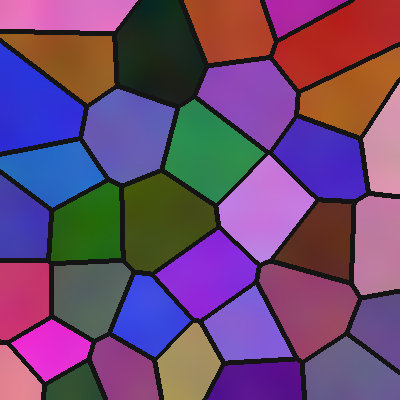
\includegraphics[width=11mm]{assets/drawn/grain-map}};
      \node[small label,text=udsdark] at ({\i*49+23},-12.9) {vs};}
    \node[pair image] at (28.6,-7.4) {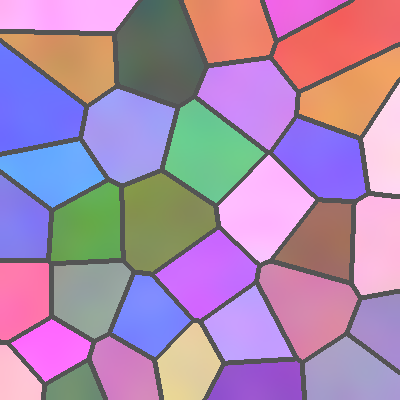
\includegraphics[width=11mm]{assets/drawn/ssim-bright}};
    \node[pair image] at (77.6,-7.4) {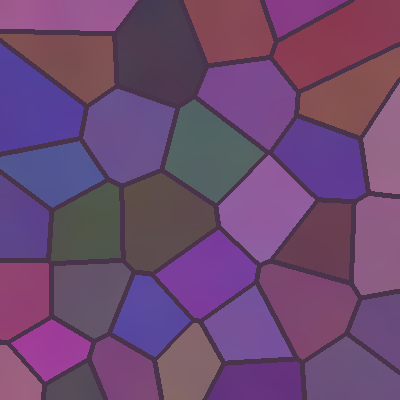
\includegraphics[width=11mm]{assets/drawn/ssim-flat}};
    \node[pair image] at (126.6,-7.4) {
\includegraphics[width=11mm]{assets/drawn/ssim-shuffled}};
    \node[component value] at (23,-19.6)
      {\textcolor{udsred}{$L=\ssimBrightL$}\enspace $C=\ssimBrightC$\enspace $S=\ssimBrightS$};
    \node[component value] at (72,-19.6)
      {$L=\ssimFlatL$\enspace \textcolor{udsred}{$C=\ssimFlatC$}\enspace $S=\ssimFlatS$};
    \node[component value] at (121,-19.6)
      {$L=\ssimShuffledL$\enspace $C=\ssimShuffledC$\enspace \textcolor{udsred}{$S=\ssimShuffledS$}};
    \node[component formula] at (23,-23.2) {$\dfrac{2\mu_x\mu_{\hat x}+C_1}{\mu_x^2+\mu_{\hat x}^2+C_1}$};
    \node[component formula] at (72,-23.2) {$\dfrac{2\sigma_x\sigma_{\hat x}+C_2}{\sigma_x^2+\sigma_{\hat x}^2+C_2}$};
    \node[component formula] at (121,-23.2) {$\dfrac{\sigma_{x\hat x}+C_3}{\sigma_x\sigma_{\hat x}+C_3}$};
    \node[component meaning] at (23,-31) {brightness: the means $\mu$};
    \node[component meaning] at (72,-31) {contrast: the spreads $\sigma$};
    \node[component meaning] at (121,-31) {pattern: the covariance $\sigma_{x\hat x}$};
    % multiplied as the paper does, and turned into a loss
    \fill[bluetint] (0,-37.6) rectangle (144,-53.6);
    \node[anchor=west,inner sep=0pt,font=\footnotesize,text=udsdark] at (2.4,-42.6)
      {$\mathrm{SSIM}=L^{\alpha}\,C^{\beta}\,S^{\gamma}$};
    \node[anchor=west,small label,text=udsdark,text width=44mm] at (2.4,-48.8)
      {paper: $\alpha=\beta=\gamma=1$, $C_3=C_2/2$};
    \node[anchor=west,inner sep=0pt,font=\footnotesize,text=udsdark] (eq8) at (46.6,-45.6)
      {$=\dfrac{(2\mu_x\mu_{\hat x}+C_1)(2\sigma_{x\hat x}+C_2)}{(\mu_x^2+\mu_{\hat x}^2+C_1)(\sigma_x^2+\sigma_{\hat x}^2+C_2)}$};
    \draw[flow,draw=udsblue] ([xshift=1.6mm]eq8.east) -- ++(5.4,0);
    \node[anchor=west,inner sep=0pt,font=\footnotesize,text=udsdark] (loss) at ([xshift=8.6mm]eq8.east)
      {$L_{\mathrm{SSIM}}=1-\mathrm{SSIM}$};
    \node[anchor=north west,small label,text=udsdark] at ([yshift=-1.4mm]loss.south west) {zero for identical patches};
  \end{tikzpicture}
  \note{\textbf{15:30--16:40}\par
    SSIM compares two patches in three ways, each through one statistic of the pixel values.\par
    Luminance compares the means: a brighter copy of the patch scores $L=\ssimBrightL$, while $C$ and $S$
      stay near 1.\par
    Contrast compares the standard deviations: a flattened copy scores $C=\ssimFlatC$.\par
    Structure compares the patterns through the covariance: shuffling the patch's tiles keeps its mean
      and spread but drops $S$ to \ssimShuffledS.\par
    The product, with all exponents 1 and $C_3=C_2/2$ as in the paper, gives its Eq.~8; the loss is one
      minus SSIM.\par
    The brighter copy differs by \ssimBrightM{} per pixel on average and keeps SSIM \ssimBrightQ; the blurred
      patch of slide 4 differs by only \ssimBlurredM{} but drops to \ssimBlurredQ: SSIM sees lost structure
      that a pixel loss barely notices.}
\end{frame}

% --------------------------------------------------- failure case, fixed
\begin{frame}[source={Liao et al.\ (2026), Nat.\ Commun.\ 17, 11232, Fig.\ 2c (CC BY-NC-ND 4.0)}]
  {The same patches, with the new loss}
  \begin{tikzpicture}[x=1mm,y=1mm]
    \useasboundingbox (0,0) rectangle (144,-54);
    \figpart{36}{0}{2}{340}{770}{1897}{1537}{104}
    \node[anchor=east,label text,align=right] at (33,{\fpy{884}}) {real patches};
    \node[anchor=east,label text,align=right,text=udsred] at (33,{\fpy{1155}}) {pixel loss only};
    \node[anchor=east,label text,align=right,text=testgreen] at (33,{\fpy{1423}}) {with edge and\\SSIM terms};
  \end{tikzpicture}
  \note{\textbf{16:40--17:20}\par
    The same six test patches, with a third row: the model trained with all three terms.\par
    The boundaries are sharp again, and each grain has nearly one colour.\par
    The pixel loss itself also falls, from about 0.20 to about 0.10 according to the text; the plotted
      curve settles nearer 0.07.\par
    Two more reconstruction terms also weaken the Kullback--Leibler term relative to the rest, which by
      itself can lower a VAE's reconstruction error; the paper does not separate the two effects.\par
    The comparison with a standard VAE, a Wasserstein GAN and a standard DDPM is only in the
      Supplementary Information.}
\end{frame}

% ------------------------------------------------------------ descriptor
\begin{frame}[source={Liao et al.\ (2026), Nat.\ Commun.\ 17, 11232, after Fig.\ 4a and Methods · Pearson (1901), Philos.\ Mag.\ 2, 559}]{Six numbers per alloy}
  \begin{tikzpicture}[x=1mm,y=1mm]
    \useasboundingbox (0,0) rectangle (144,-54);
    \tikzset{dims/.style={anchor=north,small label,text=udsdark,align=center},
      op/.style={small label,text=udsgrey,align=center},
      back/.style={anchor=north,small label,text=udsred,align=center}}
    % one alloy's map, cut into 10 x 8 patches of 100 x 100 pixels
    \node[anchor=north west,inner sep=0pt] at (0,0) {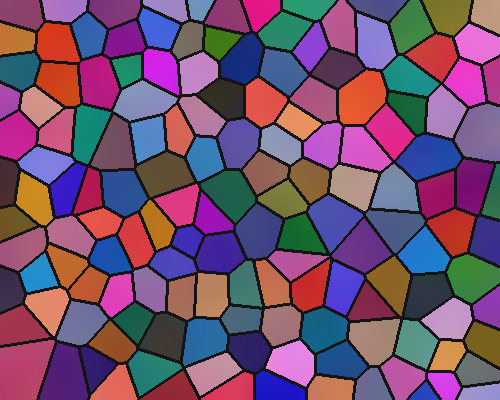
\includegraphics[width=25mm]{assets/drawn/grain-map-wide}};
    \draw[white,line width=0.35pt] \foreach \i in {1,...,9} {(\i*2.5,0) -- (\i*2.5,-20)}
      \foreach \j in {1,...,7} {(0,-\j*2.5) -- (25,-\j*2.5)};
    \node[dims] at (12.5,-20.8) {one alloy, $1000\times800$ px:\\ 80 patches};
    % the encoder gives one code of 128 numbers per patch
    \draw[flow] (25.6,-10) -- (28.2,-10);
    \filldraw[fill=bluetint,draw=udsblue,line width=0.5pt] (28.8,-3.4) -- (36.4,-6.8) -- (36.4,-13.2) -- (28.8,-16.6) -- cycle;
    \node[label text,rotate=90,font=\scriptsize] at (32.4,-10) {encoder};
    \draw[flow] (37,-10) -- (39.6,-10);
    \codematrix{40.2}{-1}{16}{18}{1}
    \node[dims] at (48.2,-20.8) {80 codes\\ $\times$ 128 numbers};
    % mean and spread over the 80 patches
    \draw[flow] (56.8,-7.2) -- node[above=0.4mm,op,sloped] {mean} (65.4,-5.4);
    \draw[flow] (56.8,-12.8) -- node[below=0.4mm,op,sloped] {spread} (65.4,-14.6);
    \pgfmathsetseed{80}
    \foreach \c in {0,...,15} {
      \pgfmathtruncatemacro\shadeA{20+50*rnd}
      \pgfmathtruncatemacro\shadeB{10+45*rnd}
      \filldraw[fill=udsblue!\shadeA,draw=udsblue,line width=0.3pt] ({66+1.25*\c},-4.2) rectangle ++(1.25,-2.4);
      \filldraw[fill=udsdark!\shadeB,draw=udsdark,line width=0.3pt] ({66+1.25*\c},-13.4) rectangle ++(1.25,-2.4);}
    \node[anchor=south,small label,text=udsdark] at (76,-3.6) {$\mu$: 128 numbers};
    \node[dims] at (76,-16.4) {$\sigma$: 128 numbers};
    % PCA, fitted on the 25 alloys: the first three components of each
    \draw[flow] (86.6,-5.4) -- node[above=0.4mm,op] {PCA} (92.4,-5.4);
    \draw[flow] (86.6,-14.6) -- node[below=0.4mm,op] {PCA} (92.4,-14.6);
    \foreach \j in {0,1,2} {
      \filldraw[fill=bluetint,draw=udsblue,line width=0.5pt] ({93+2.4*\j},-4.2) rectangle ++(2.4,-2.4);
      \filldraw[fill=darktint,draw=udsdark,line width=0.5pt] ({93+2.4*\j},-13.4) rectangle ++(2.4,-2.4);}
    \node[op,anchor=north] at (96.6,-19.6) {first 3 of\\ 24 components};
    % the descriptor
    \draw[flow] (100.8,-5.4) to[out=0,in=180] (107.4,-9.4);
    \draw[flow] (100.8,-14.6) to[out=0,in=180] (107.4,-10.6);
    \descstrip{108}{-8.8}{2.4}{2.4}
    \node[anchor=south,small label,text=udsdark] at (115.2,-8.2) {descriptor};
    \node[anchor=west,small label,text=udsdark] at (123.2,-10) {6 numbers};
    % the table it fills: one row per alloy, beside the measured properties
    \draw[flow] (115.2,-11.6) -- (115.2,-31.8);
    \descstrip{108}{-32.4}{2.4}{3}
    \foreach \x/\l in {122.4/YS,129.4/El}
      \node[draw=udsgreymid,fill=darktint,line width=0.3pt,minimum width=7mm,minimum height=3mm,inner sep=0pt,
        anchor=north west,font=\scriptsize,text=udsdark] at (\x,-32.4) {\l};
    \foreach \r in {1,...,3} \foreach \x/\w in {108/14.4,122.4/7,129.4/7}
      \draw[udsgreylight,line width=0.3pt,fill=white] (\x,{-32.4-3*\r}) rectangle ++(\w,-3);
    \node[small label,text=udsdark] at (122.4,-45.4) {$\vdots$};
    \node[dims,text width=36mm] at (122.4,-48.9) {25 alloys: six numbers, yield strength, elongation};
    % the way back, which the search uses: below the labels, up to the map's label at the end
    \draw[udsred,line width=0.6pt,dash pattern=on 1.6pt off 1.2pt,-{Stealth[length=1.6mm,width=1.2mm]}]
      (109.2,-11.6) -- (109.2,-31) -- (12.5,-31) -- (12.5,-27.6);
    \foreach \x/\l in {96.6/inverse PCA,76/{$\mu$, $\sigma$},48.2/draw 80 codes,32.6/decode}
      \node[back] at (\x,-31.8) {\l};
    \node[anchor=north west,small label,text=udsred,text width=92mm] at (0,-36.4)
      {the way back, for the search: six numbers give a mean and a spread, 80 codes are drawn from them and
       decoded into new patches};
  \end{tikzpicture}
  \note{\textbf{17:20--18:10}\par
    To link microstructures with properties, each alloy needs one descriptor.\par
    The 80 patches of its map are encoded, which gives 80 codes of 128 numbers.\par
    Their mean and standard deviation over the patches describe the alloy: what its patches look like
      on average, and how much they vary.\par
    Principal component analysis (PCA, Pearson 1901), fitted on the 25 alloys, keeps the first three of
      24 components of each, so every alloy becomes six numbers beside its measured properties.\par
    PCA can be inverted, the red path: six numbers map back to a mean and a spread, from which new codes
      are drawn and decoded.\par
    The number of components was chosen by the fidelity of the generated patches (Supplementary
      Information).}
\end{frame}

% ---------------------------------------------------------------- search
\begin{frame}[source={Liao et al.\ (2026), Nat.\ Commun.\ 17, 11232, after Fig.\ 4a · Deb et al.\ (2002), IEEE Trans.\ Evol.\ Comput.\ 6, 182}]{A genetic search in six numbers}
  \begin{tikzpicture}[x=1mm,y=1mm]
    \useasboundingbox (0,0) rectangle (144,-54);
    \tikzset{glyph label/.style={anchor=north,small label,text=udsdark,align=center},
      op/.style={anchor=south,small label,text=udsgrey,align=center,yshift=1mm}}
    % the loop: four steps on cards, run for 500 generations
    \foreach \i/\h in {0/population,1/predict,2/keep the best,3/{cross over, mutate}} {
      \pgfmathsetmacro\cx{\i*38}
      \fill[bluetint] (\cx,-5.4) rectangle ++(30,-13.4);
      \cardhead{\cx}{0}{30}{udsblue}{\h}}
    \foreach \i in {0,1,2} \draw[flow,draw=udsblue] ({\i*38+30.4},-12.1) -- ({\i*38+37.6},-12.1);
    % population: 10 descriptors of six numbers
    \foreach \k in {0,...,4} {\descstrip{4}{-7-1.7*\k}{1.5}{1.2}\descstrip{17}{-7-1.7*\k}{1.5}{1.2}}
    \node[glyph label] at (15,-15.6) {10 descriptors};
    % predict: one tree model per property
    \minitree{45.5}{-7.2}
    \minitree{60.5}{-7.2}
    \node[glyph label] at (45.5,-14.2) {strength};
    \node[glyph label] at (60.5,-14.2) {elongation};
    % keep the best: fronts and crowding, as on slide 10
    \begin{scope}[shift={(80.5,-17.4)}]
      \draw[udsgreymid,line width=0.4pt] (0,10.4) -- (0,0) -- (22,0);
      \begin{scope}[x=22mm,y=10mm]
        \drawfronttwo[udsgreymid,line width=0.5pt,dash pattern=on 1.2pt off 0.9pt]
        \drawfrontone[udsblue,line width=0.7pt]
        \foreach \x/\y/\r in \paretopoints {
          \ifcase\r\or\def\rc{udsblue}\or\def\rc{udsgreymid}\else\def\rc{udsgreylight}\fi
          \node[circle,fill=\rc,inner sep=0pt,minimum size=1.2mm] at (\x,\y) {};}
      \end{scope}
    \end{scope}
    % cross over and mutate: a child from two parents, one number changed
    \foreach \j in {0,...,5} {
      \filldraw[fill=udsblue!20,draw=udsblue,line width=0.3pt] ({116.6+1.8*\j},-7.4) rectangle ++(1.8,-1.8);
      \filldraw[fill=udsblue!65,draw=udsblue,line width=0.3pt] ({116.6+1.8*\j},-10.4) rectangle ++(1.8,-1.8);
      \ifnum\j<3\def\cf{udsblue!20}\else\def\cf{udsblue!65}\fi
      \ifnum\j=4\def\cf{udsred!70}\fi
      \filldraw[fill=\cf,draw=udsblue,line width=0.3pt] ({131.4+1.8*\j},-8.9) rectangle ++(1.8,-1.8);}
    \draw[flow,draw=udsblue,line width=0.5pt] (128.4,-9.8) -- (130.8,-9.8);
    \node[glyph label] at (122,-13.4) {parents};
    \node[glyph label] at (136.8,-13.4) {child, one\\ number mutated};
    % 500 generations: the way round
    \draw[flow,draw=udsblue] (129,-18.8) -- (129,-21.8) -- (15,-21.8) -- (15,-19.2);
    \node[fill=white,inner sep=1mm,font=\footnotesize\bfseries,text=udsblue] at (72,-21.8) {500 generations};
    % the way back to microstructures, for the 5 best
    \draw[flow] (5,-18.8) -- (5,-30.8);
    \node[anchor=west,small label,text=udsdark] at (6.4,-25) {the 5 best};
    \foreach \k in {0,...,4} \descstrip{0}{-31.4-1.8*\k}{1.8}{1.3}
    \node[glyph label] at (5.4,-41.6) {5 descriptors};
    \draw[flow] (12.2,-36) -- node[op] {inverse\\ PCA} (26.4,-36);
    \pgfmathsetseed{80}
    \foreach \c in {0,...,15} {
      \pgfmathtruncatemacro\shadeA{20+50*rnd}
      \pgfmathtruncatemacro\shadeB{10+45*rnd}
      \filldraw[fill=udsblue!\shadeA,draw=udsblue,line width=0.3pt] ({27.2+1.25*\c},-32.6) rectangle ++(1.25,-2.4);
      \filldraw[fill=udsdark!\shadeB,draw=udsdark,line width=0.3pt] ({27.2+1.25*\c},-37) rectangle ++(1.25,-2.4);}
    \node[glyph label] at (37.2,-40.2) {$\mu$, $\sigma$: 128 each};
    \draw[flow] (48,-36) -- node[op] {draw\\ 80 codes} (62.2,-36);
    \codematrix{63}{-30.6}{12}{11}{1}
    \node[glyph label] at (69,-42.4) {80 codes};
    \draw[flow] (75.8,-36) -- node[op] {decode,\\ refine} (90,-36);
    \node[anchor=north west,inner sep=0pt] at (90.8,-29.6) {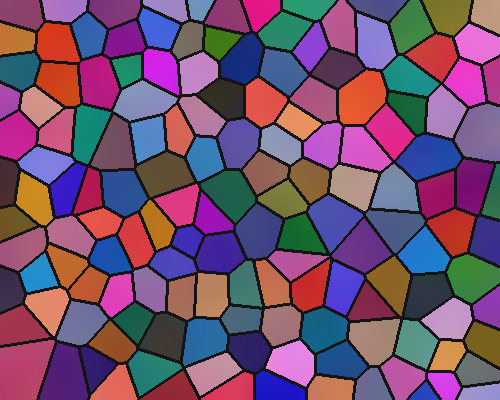
\includegraphics[width=25mm]{assets/drawn/grain-map-wide}};
    \draw[white,line width=0.35pt] \foreach \i in {1,...,9} {(90.8+\i*2.5,-29.6) -- (90.8+\i*2.5,-49.6)}
      \foreach \j in {1,...,7} {(90.8,-29.6-\j*2.5) -- (115.8,-29.6-\j*2.5)};
    \node[glyph label] at (103.3,-50.2) {80 new patches};
    \node[text=udsred,font=\small] at (120.2,-34.4) {\faStar};
    \node[anchor=north west,label text,text width=21mm,text=udsred] at (122.6,-32.4)
      {a proposed microstructure for each descriptor};
  \end{tikzpicture}
  \note{\textbf{18:10--19:00}\par
    The loop of section 2, run on the six numbers.\par
    Two gradient-boosted tree models, one per property, fitted on the 20 training alloys, predict yield
      strength and elongation from a descriptor; they are the objectives.\par
    NSGA-II evolves a population of 10 descriptors over 500 generations; the paper's average hypervolume
      improvement, the area the candidates span above the weakest measured alloy, levels off after about
      150 generations.\par
    The five best final descriptors go back through the inverse PCA to a mean and a spread; 80 codes are
      drawn from them and decoded into patches, the proposed microstructures.}
\end{frame}

\section[Results]{The results}
\sectionframe{04}{The results}{What do the authors show?}{\faChartBar}

% ------------------------------------------------------------ fidelity
\begin{frame}[source={Liao et al.\ (2026), Nat.\ Commun.\ 17, 11232, Fig.\ 3i--n (CC BY-NC-ND 4.0)}]
  {Grain statistics after reconstruction}
  \begin{tikzpicture}[x=1mm,y=1mm]
    \useasboundingbox (0,0) rectangle (144,-54);
    \figpart{0}{0}{3}{0}{700}{2000}{1883}{91}
    % the two rows of panels, by the figure's own panel letters
    \node[anchor=north west,label text,text width=46mm] at (98,-0.6) {original against reconstruction};
    \node[anchor=west,label text,text width=46mm] at (98,-8.4) {\textbf{i--k}\enspace grain area and ellipse axes};
    \node[anchor=west,label text,text width=46mm] at (98,-13.8) {\textbf{l--n}\enspace the three Euler angles};
    \node[circle,fill=udsgreylight,inner sep=0pt,minimum size=2mm] at (99.4,-20.6) {};
    \node[anchor=west,label text,text width=41mm] at (102,-20.6) {2,000 single patches: wide scatter};
    \node[circle,fill=udsblue!75,inner sep=0pt,minimum size=2mm] at (99.4,-27.4) {};
    \node[anchor=west,label text,text width=41mm] at (102,-27.4) {20 training alloys, each the mean of 80 patches};
    \node[rectangle,fill=udsred!80,inner sep=0pt,minimum size=2mm] at (99.4,-34.2) {};
    \node[anchor=west,label text,text width=41mm] at (102,-34.2) {5 test alloys};
    \draw[udsred,line width=0.6pt,dash pattern=on 1.4pt off 1pt] (98,-39.6) -- (100.8,-39.6);
    \node[anchor=west,label text] at (102,-39.6) {reconstruction = original};
  \end{tikzpicture}
  \note{\textbf{19:10--20:00}\par
    Six features are measured in each original patch and its reconstruction: grain area, the major
      and minor axes of the equivalent ellipse (panels i to k), and the three Euler angles (l to n).\par
    The grey points are the 2,000 single patches; their means scatter widely, more so for large grains,
      of which one patch holds only a few.\par
    Averaged over the 80 patches of each alloy, the 20 training alloys in blue and the 5 test alloys in
      red lie on the line of equality.\par
    So the model reproduces the grain statistics of alloys it never saw.\par
    What is compared: reconstructions with their own inputs, the first task of slide 7.\par
    Misorientation statistics and the baseline models are in the Supplementary Information only.}
\end{frame}

% ---------------------------------------------------------- surrogates
\begin{frame}[source={Liao et al.\ (2026), Nat.\ Commun.\ 17, 11232, Fig.\ 4b, c (CC BY-NC-ND 4.0) · Friedman (2001), Ann.\ Stat.\ 29, 1189}]
  {Property predictions}
  \begin{tikzpicture}[x=1mm,y=1mm]
    \useasboundingbox (0,0) rectangle (144,-54);
    \figpart{6}{0}{4}{0}{480}{640}{975}{62}
    \figpart{78}{0}{4}{640}{480}{1260}{975}{60.1}
    \node[anchor=north west,label text,text width=144mm] at (6,-50)
      {Gradient-Boosted Trees on the six numbers: fitted on 20 alloys, tested on 5};
  \end{tikzpicture}
  \note{\textbf{20:00--20:40}\par
    These are two gradient-boosted tree models (Friedman, 2001), one per property: sums of many small
      regression trees on an alloy's six numbers; the number of trees and their depth were set by a
      randomized search.\par
    On the five test alloys, R² is 0.96 for yield strength and 0.92 for elongation; on the 20 training
      alloys 0.96 and 0.93.\par
    R² is the share of the variance of the measured values that the predictions explain.\par
    These two models are what the search optimizes.}
\end{frame}

% ---------------------------------------------------------- candidates
\begin{frame}[source={Liao et al.\ (2026), Nat.\ Commun.\ 17, 11232, after Fig.\ 4f; Fig.\ 4e (CC BY-NC-ND 4.0)}]
  {Five candidates beyond the front}
  \begin{tikzpicture}[x=1mm,y=1mm]
    \useasboundingbox (0,0) rectangle (144,-54);
    \begin{scope}[shift={(14,-41)}]
      \planeaxes{340}{1000}{28}{86}{76}{41}{400,500,...,1000}{30,40,...,80}
      \begin{scope}[plane]
        \drawfront[front]
        \drawalloys
        \drawcandidates
        \node[anchor=west,inner sep=0pt] at ([xshift=1.4mm]cand1.east) {\candlabel{1}};
        \node[anchor=west,inner sep=0pt] at ([xshift=1.4mm]cand2.east) {\candlabel{2}};
      \end{scope}
      \node[alloy] at (52,39.4) {};
      \node[anchor=west,small label,text=udsdark] at (54,39.4) {measured};
      \node[candidate] at (52,35.4) {};
      \node[anchor=west,small label,text=udsdark] at (54,35.4) {candidates};
    \end{scope}
    \node[axis label] at (52,-48.4) {yield strength (MPa)};
    \node[axis label,rotate=90] at (3,-20.5) {elongation (\%)};
    % the latent plane of Fig. 4e
    \figpart{95}{0}{4}{1280}{480}{2000}{975}{49}
    \node[anchor=north west,small label,text width=49mm] at (95,-35.6)
      {first principal components of mean and spread: generated (red) beside measured (grey)};
  \end{tikzpicture}
  \note{\textbf{20:40--21:40}\par
    After 500 generations the search returns five candidates, here with their predicted properties.\par
    All five lie above the measured front: at equal strength, they are predicted to stretch more.\par
    Their predicted values stay inside the ranges of the 25 measured alloys; the gain lies in their
      combination.\par
    On the right, the first principal components of the mean and the spread: measured alloys in grey,
      generated microstructures as triangles, darker for a larger hypervolume improvement.\par
    The best candidates lie far from every measured alloy; the authors call them out of distribution,
      the third task of slide 7.\par
    Candidates 1 and 2 are the ones checked by simulation.}
\end{frame}

% --------------------------------------------------------- fine grains
\begin{frame}[source={Liao et al.\ (2026), Nat.\ Commun.\ 17, 11232, Fig.\ 5a--d (CC BY-NC-ND 4.0) · Ma and Zhu (2017), Mater.\ Today 20, 323}]
  {Fine grains in the generated patches}
  \begin{tikzpicture}[x=1mm,y=1mm]
    \useasboundingbox (0,0) rectangle (144,-54);
    \figpart{0}{0}{5}{0}{0}{1300}{965}{72}
    % generated patches and their histogram, by the figure's own panel letters
    \node[anchor=west,label text,text width=60mm] at (80,-2.6) {\textbf{b}\enspace fine-grain regions, marked by arrows};
    \node[anchor=west,label text,text width=60mm] at (80,-8) {\textbf{d}\enspace more grains in the smallest bin};
    % the proposed mechanism, on an illustrative map
    \node[anchor=north west,small label] at (80,-13.6) {proposed mechanism};
    \node[anchor=north west,inner sep=0pt] (bm) at (80,-17.4) {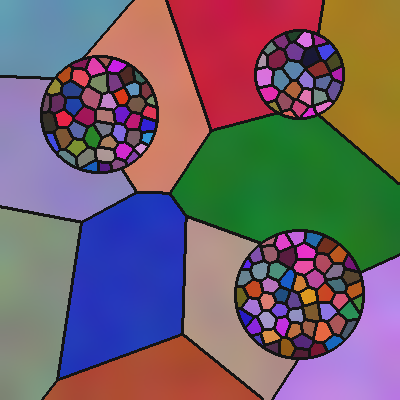
\includegraphics[width=20mm]{assets/drawn/grain-map-bimodal}};
    \node[anchor=west,label text] (fine) at (104,-21.4) {fine grains};
    \draw[udsdark,line width=0.4pt] (fine.west) -- ++(-1.6,0) -- (95,-21.15);
    \node[anchor=west,label text] (coarse) at (104,-28.4) {coarse grains};
    \draw[udsdark,line width=0.4pt] (coarse.west) -- ++(-1.6,0) -- (98,-26.9);
    \node[anchor=north west,card text,text width=63mm] at (80,-39.6)
      {\cardbullet{fine grains block dislocations: strength}
       \cardbullet{coarse grains let them glide: ductility}
       \cardbullet{the mismatch stores dislocations: hardening}};
  \end{tikzpicture}
  \note{\textbf{21:40--22:40}\par
    Left, patches of the initial alloys and patches generated for the candidates; the arrows mark what
      the authors call fine-grain regions (panel b).\par
    Below, the grain areas of all 2,000 original patches and of 400 generated ones, on a logarithmic
      axis: the generated patches have more grains in the smallest bin, at or below 0.4 µm² (panel d),
      which the authors read as a bimodal grain size.\par
    Their explanation: fine grains block dislocations and raise the strength, coarse grains leave room
      for them to glide and keep the ductility, and the mismatch between the two stores geometrically
      necessary dislocations (GNDs), which raise the strain hardening.\par
    The mechanism is established for heterogeneous microstructures; whether these generated patches
      show it remains to be checked.}
\end{frame}

% ------------------------------------------------------------ validation
\begin{frame}[source={Liao et al.\ (2026), Nat.\ Commun.\ 17, 11232, Fig.\ 5e, h (CC BY-NC-ND 4.0)}]
  {Simulation and one experiment}
  \begin{tikzpicture}[x=1mm,y=1mm]
    \useasboundingbox (0,0) rectangle (144,-54);
    \figpart{0}{0}{5}{1430}{49}{1908}{434}{54}
    \node[anchor=north west,label text,text width=54mm] at (0,-46.6)
      {new alloy, route from the literature: 60\,\% rolling at 1000\,°C, 5\,min at 850\,°C};
    \figpart{60}{0}{5}{660}{972}{2000}{1473}{84}
    \node[anchor=north west,label text,text width=84mm] at (60,-33.6)
      {candidate \candlabel{1}: i predicted, ii simulated by crystal plasticity (CPFE), iii measured on
       the new alloy};
  \end{tikzpicture}
  \note{\textbf{22:40--23:40}\par
    Two checks follow.\par
    First, crystal plasticity finite element (CPFE) simulations of two generated patches per candidate,
      with a slip model calibrated on three measured stress--strain curves; the Euler angles come from
      the pixel colours, the dislocation density from a learned mapping.\par
    Second, one experiment: an alloy processed by a route the authors chose from the literature to get
      a bimodal grain size, 60 percent hot rolling at 1000 °C and 5 minutes at 850 °C.\par
    Its EBSD map, left, shows coarse grains among many fine ones.\par
    Right, candidate 1 as predicted, simulated and measured: yield strength about 820, 805 and 825 MPa,
      elongation about 48, 44.5 and 43.5 percent, read from the bars.\par
    The paper concludes that the design is validated.}
\end{frame}

% --------------------------------------------------------------- thank you
% the thanks where the title slide has its title; drawn inside the frame, so that the notes' thumbnail
% shows it too
\begin{frame}[plain,noframenumbering]
\vbox to 0pt{\vskip-2mm\hbox to 0pt{\hskip-8mm\begin{tikzpicture}[x=1mm,y=1mm]
  \useasboundingbox (0,0) rectangle (160,-90);
  \node[anchor=north west,inner sep=0pt] at (8,-8) {\includegraphics[width=30mm]{\udslogo}};
  \node[anchor=north west,inner sep=0pt,text width=88mm,align=left] at (8,-36) {%
    {\fontsize{32}{36}\selectfont\bfseries\color{udsblue}Thank you\par}\vskip4mm
    \textcolor{udsred}{\rule{14mm}{0.8pt}}\par\vskip3mm
    {\fontsize{11}{13}\selectfont\color{udsdark}\insertauthor\par}};
\end{tikzpicture}\hss}\vss}
\par\rule{0pt}{80mm}
\note{\textbf{23:40--24:00}\par
    Thank you.\par
    Questions to open the discussion: would edge and SSIM terms help our segmentation of grain
      boundaries; what minimum grain size do we use in EBSD analysis, and why; how many independent
      specimens would we want before trusting a property model; and what would convince us that a
      generated microstructure is new and can be made.\par
    Backup slides follow: the loss terms in full, the 25 processing routes and the references.}
\end{frame}

\appendix
% the footer numbers appendix slides A1, A2, ..., as their titles do
\setcounter{framenumber}{0}
\renewcommand\insertframenumber{A\arabic{framenumber}}
% Appendix: its own sections, so the mini-frame headline shows only these.
\section[Backup]{Backup}

% ------------------------------------------------------------ loss terms
\begin{frame}[source={Liao et al.\ (2026), Nat.\ Commun.\ 17, 11232, Eqs.\ 2--15}]{A1\enspace The loss terms in full}
  \begin{columns}[T,onlytextwidth]
    \begin{column}{0.48\textwidth}
      \small
      {\scriptsize\color{udsgrey}Sobel kernels and edge term (Eqs.\ 2, 3)}
      \[ S_x=\left[\begin{array}{rrr}-1&0&1\\-2&0&2\\-1&0&1\end{array}\right],\;\;
         S_y=\left[\begin{array}{rrr}-1&-2&-1\\0&0&0\\1&2&1\end{array}\right] \]
      \[ L_{\mathrm{edge}}=\mathrm{mean}\big(|S_x\ast x-S_x\ast\hat{x}|+|S_y\ast x-S_y\ast\hat{x}|\big) \]
      {\scriptsize\color{udsgrey}structural similarity (Eqs.\ 8, 9)}
      \[ \mathrm{SSIM}(x,\hat{x})=\frac{(2\mu_x\mu_{\hat{x}}+C_1)(2\sigma_{x\hat{x}}+C_2)}
         {(\mu_x^2+\mu_{\hat{x}}^2+C_1)(\sigma_x^2+\sigma_{\hat{x}}^2+C_2)} \]
      \[ L_{\mathrm{SSIM}}=1-\mathrm{SSIM}(x,\hat{x}) \]
    \end{column}
    \begin{column}{0.48\textwidth}
      \small
      {\scriptsize\color{udsgrey}VAE, with $x_V$ the reconstruction of $x$ (Eq.\ 11)}
      \[ L_{\mathrm{VAE}}=L_{\mathrm{pix}}+L_{\mathrm{edge}}+L_{\mathrm{SSIM}}+L_{\mathrm{KL}}\big(q(z|x),p(z)\big) \]
      {\scriptsize\color{udsgrey}diffusion: forward process (Eq.\ 13)}
      \[ q(x_t|x)=\mathcal{N}\big(x_t;\sqrt{\bar{\alpha}_t}\,x,(1-\bar{\alpha}_t)\mathbf{I}\big) \]
      {\scriptsize\color{udsgrey}diffusion: loss on the predicted noise $\epsilon_\theta(x_t,t,x_V)$ (Eq.\ 15)}
      \[ L_{\mathrm{DDPM}}=L_{\mathrm{pix}}(\epsilon_\theta,\tilde{\epsilon})+L_{\mathrm{SSIM}}(\epsilon_\theta,\tilde{\epsilon})
         +L_{\mathrm{edge}}(\epsilon_\theta,\tilde{\epsilon}) \]
    \end{column}
  \end{columns}
  \note{\textbf{If asked}\par
    The pixel, edge and SSIM terms are added without weights, in the VAE and in the diffusion model.\par
    In the diffusion model they compare the predicted with the true noise, so their link to grain
      boundaries is indirect.\par
    Eq.\ 14 as printed gives the predicted noise as the mean of the reverse step; standard DDPM sampling
      derives that mean from the predicted noise.\par
    SSIM uses its three factors (luminance, contrast, structure) with equal exponents of one, which
      gives Eq.\ 8; $C_1$ and $C_2$ are small constants.}
\end{frame}

% ----------------------------------------------------------------- the data
\begin{frame}[source={Liao et al.\ (2026), Nat.\ Commun.\ 17, 11232}]{A2\enspace The 25 processing routes}
  \scriptsize\renewcommand\arraystretch{1.08}\setlength\tabcolsep{6pt}
  \def\alloyhead{\toprule
      & \multicolumn{2}{c}{annealing} & rolling & \multicolumn{2}{c}{measured}\\
    ID & °C & h & \% & MPa & \%\\
    \midrule}
  \hfill
  \begin{tabular}[t]{@{}rrrrrr@{}}
    \alloyhead
    \alloytableA
    \bottomrule
  \end{tabular}\hfill\hfill
  \begin{tabular}[t]{@{}rrrrrr@{}}
    \alloyhead
    \alloytableB
    \bottomrule
  \end{tabular}\hfill\null
  \note{\textbf{If asked}\par
    The table of the code repository: each variant's processing route, hot rolling at 900 °C and then
      annealing, with its measured yield strength and elongation.\par
    Every pair of levels occurs once: an orthogonal design.\par
    Alloy 10 is the measured alloy closest in strength to candidate 1.\par
    The paper's 20/5 split is random and not listed; from Fig.\ 4b, the test alloys lie near 375, 445,
      470, 795 and 845 MPa.}
\end{frame}

\section[References]{References}

\begin{frame}{A3\enspace References}
  \begin{columns}[T,onlytextwidth]
  \begin{column}{0.53\textwidth}
  \scriptsize\setlength\parskip{0.6mm}\raggedright
  \textbf{The paper and its code}\par
  W.~Liao, K.~Li, B.~Tang, J.~Fan, J.~Wang, X.~Xue, J.~Li, R.~Yuan (2026). \emph{Generative design of high-fidelity
  microstructures using physics-aware machine learning}. Nature Communications 17, 11232.
  \url{https://doi.org/10.1038/s41467-026-78118-3}, CC~BY-NC-ND~4.0.\par
  W.~Liao, R.~Yuan (2026). \emph{microstructures\_design}, code, trained models and \fn{dataset.csv}, commit 25f6017,
  MIT licence, read 4~Nov~2026.\\ \url{https://github.com/nwpuai4msegroup/microstructures_design};\\ archived at
  \url{https://doi.org/10.5281/zenodo.21897025}.\par
  \textbf{Materials background}\par
  E.~Ma, T.~Zhu (2017). \emph{Towards strength--ductility synergy through the design of heterogeneous nanostructures
  in metals}. Materials Today 20(6), 323--331.\par
  \end{column}
  \begin{column}{0.43\textwidth}
  \scriptsize\setlength\parskip{0.4mm}\raggedright
  \textbf{Generative models}\par
  D.~P.~Kingma, M.~Welling (2013). \emph{Auto-encoding variational Bayes}. arXiv:1312.6114; ICLR 2014.\par
  I.~Goodfellow et al.\ (2014). \emph{Generative adversarial nets}. NeurIPS~27.\par
  J.~Sohl-Dickstein, E.~Weiss, N.~Maheswaranathan, S.~Ganguli (2015). \emph{Deep unsupervised learning using
  nonequilibrium thermodynamics}. ICML 2015, PMLR 37, 2256--2265.\par
  J.~Ho, A.~Jain, P.~Abbeel (2020). \emph{Denoising diffusion probabilistic models}. NeurIPS~33.\par
  A.~Ramesh et al.\ (2021). \emph{Zero-shot text-to-image generation}. ICML 2021, PMLR 139, 8821--8831.\par
  R.~Rombach, A.~Blattmann, D.~Lorenz, P.~Esser, B.~Ommer (2022). \emph{High-resolution image synthesis with latent
  diffusion models}. CVPR 2022, 10684--10695.\par
  K.~Pandey, A.~Mukherjee, P.~Rai, A.~Kumar (2022). \emph{DiffuseVAE: efficient, controllable and high-fidelity
  generation from low-dimensional latents}. Transactions on Machine Learning Research.\par
  \end{column}
  \end{columns}
\end{frame}

\begin{frame}{A4\enspace References}
  \begin{columns}[T,onlytextwidth]
  \begin{column}{0.48\textwidth}
  \scriptsize\setlength\parskip{0.6mm}\raggedright
  \textbf{Image processing}\par
  I.~Sobel, G.~Feldman (1968). \emph{A 3\,×\,3 isotropic gradient operator for image processing}. Talk at the Stanford
  Artificial Intelligence Project.\par
  Z.~Wang, A.~C.~Bovik, H.~R.~Sheikh, E.~P.~Simoncelli (2004). \emph{Image quality assessment: from error visibility
  to structural similarity}. IEEE Transactions on Image Processing 13(4), 600--612.\par
  O.~Ronneberger, P.~Fischer, T.~Brox (2015). \emph{U-Net: convolutional networks for biomedical image
  segmentation}. MICCAI 2015, 234--241.\par
  \textbf{Optimization}\par
  V.~Pareto (1906). \emph{Manuale di economia politica}. Società Editrice Libraria, Milan.\par
  J.~H.~Holland (1975). \emph{Adaptation in Natural and Artificial Systems}. University of Michigan Press.\par
  K.~Deb, A.~Pratap, S.~Agarwal, T.~Meyarivan (2002). \emph{A fast and elitist multiobjective genetic algorithm:
  NSGA-II}. IEEE Transactions on Evolutionary Computation 6(2), 182--197.\par
  \end{column}
  \begin{column}{0.48\textwidth}
  \scriptsize\setlength\parskip{0.6mm}\raggedright
  \textbf{Statistics}\par
  K.~Pearson (1901). \emph{On lines and planes of closest fit to systems of points in space}. Philosophical
  Magazine 2(11), 559--572.\par
  L.~Breiman, J.~H.~Friedman, R.~A.~Olshen, C.~J.~Stone (1984). \emph{Classification and Regression Trees}.
  Wadsworth.\par
  J.~H.~Friedman (2001). \emph{Greedy function approximation: a gradient boosting machine}. Annals of Statistics
  29(5), 1189--1232.\par
  \end{column}
  \end{columns}
\end{frame}

\end{document}
.
\providecommand\notesmode{hide notes}
\setbeameroption{\notesmode}

% Plot data, crops of the paper's figures, the property plane and other drawing helpers.
% Drawing helpers of this talk, loaded after the theme.
\usetikzlibrary{decorations.pathreplacing}% braces

% Plot data: the 25 measured alloys, their front, the processing design, values read off the paper's figures,
% and the Euler colours of the colour slide; written by tools/make_assets.py.
% Written by tools/make_assets.py; edit the script, not this file.
% The 25 measured alloys (assets/liao2026/dataset.csv): yield strength (MPa)/elongation (%)/ID.
\def\alloydata{470.23/69.32/1,468.47/68.7/2,434.94/72.51/3,394.53/78.29/4,362.26/82.18/5,377.75/78.15/6,399.05/75.03/7,613.19/53.39/8,700.46/49.44/9,827.46/40.76/10,897.42/35.42/11,793.37/40.48/12,594.08/50.53/13,441.99/69.56/14,395.19/74.56/15,429.82/67.24/16,451.36/66.3/17,593.98/45.55/18,790.98/39.15/19,983.38/33.63/20,938.12/32.69/21,844.78/36.77/22,807.42/35.94/23,462.32/64.45/24,373.67/70.09/25}
% Their front: \drawfront[options] draws its staircase in (MPa,%) coordinates.
\newcommand\drawfront[1][]{\draw[#1] (362.26,82.18) -- (362.26,78.29) -- (394.53,78.29) -- (394.53,75.03) -- (399.05,75.03) -- (399.05,72.51) -- (434.94,72.51) -- (434.94,69.56) -- (441.99,69.56) -- (441.99,69.32) -- (470.23,69.32) -- (470.23,53.39) -- (613.19,53.39) -- (613.19,49.44) -- (700.46,49.44) -- (700.46,40.76) -- (827.46,40.76) -- (827.46,36.77) -- (844.78,36.77) -- (844.78,35.42) -- (897.42,35.42) -- (897.42,33.63) -- (983.38,33.63);}
% The processing design: hot-rolling reduction (%)/annealing temperature (C)/annealing time (h)/yield strength (MPa)/shade of blue (%).
\def\alloygrid{0/650/1/470/19,0/750/5/468/19,0/850/10/435/15,0/950/15/395/11,0/1050/20/362/8,20/1050/15/378/10,20/950/10/399/12,20/850/5/613/33,20/750/1/700/42,20/650/20/827/54,30/650/15/897/61,30/750/10/793/51,30/850/20/594/31,30/950/1/442/16,30/1050/5/395/11,40/1050/1/430/15,40/950/5/451/17,40/850/15/594/31,40/750/20/791/51,40/650/10/983/70,50/650/5/938/65,50/750/15/845/56,50/850/1/807/52,50/950/20/462/18,50/1050/10/374/9}
% Read off the paper's figures: the five candidates of Fig. 4f, yield strength/elongation/label (0: none),
% and candidate 1 in Fig. 5h as simulated and as measured on the processed alloy.
\def\candidatedata{556/68.8/0,666/67.6/0,677/65.3/2,823/48.1/1,899/46.5/0}
\def\predictedpoint{823,48.1}
\def\simulatedpoint{808,44.5}
\def\measuredpoint{825,43.5}
% Euler colours of nearly equal orientations: phi1 = 2 and 358 degrees (Phi 30, phi2 45), and
% phi2 = 1 and 89 degrees (phi1 120, Phi 30), which a 90-degree cubic symmetry relates.
\definecolor{wrapA}{RGB}{1,85,128}
\definecolor{wrapB}{RGB}{254,85,128}
\definecolor{symA}{RGB}{85,85,3}
\definecolor{symB}{RGB}{85,85,252}
% The 25 processing routes, rows 1-13 and 14-25: ID & C & h & % & MPa & %.
\def\alloytableA{1 & 650 & 1 & 0 & 470 & 69.3\\2 & 750 & 5 & 0 & 468 & 68.7\\3 & 850 & 10 & 0 & 435 & 72.5\\4 & 950 & 15 & 0 & 395 & 78.3\\5 & 1050 & 20 & 0 & 362 & 82.2\\6 & 1050 & 15 & 20 & 378 & 78.2\\7 & 950 & 10 & 20 & 399 & 75.0\\8 & 850 & 5 & 20 & 613 & 53.4\\9 & 750 & 1 & 20 & 700 & 49.4\\10 & 650 & 20 & 20 & 827 & 40.8\\11 & 650 & 15 & 30 & 897 & 35.4\\12 & 750 & 10 & 30 & 793 & 40.5\\13 & 850 & 20 & 30 & 594 & 50.5\\}
\def\alloytableB{14 & 950 & 1 & 30 & 442 & 69.6\\15 & 1050 & 5 & 30 & 395 & 74.6\\16 & 1050 & 1 & 40 & 430 & 67.2\\17 & 950 & 5 & 40 & 451 & 66.3\\18 & 850 & 15 & 40 & 594 & 45.5\\19 & 750 & 20 & 40 & 791 & 39.1\\20 & 650 & 10 & 40 & 983 & 33.6\\21 & 650 & 5 & 50 & 938 & 32.7\\22 & 750 & 15 & 50 & 845 & 36.8\\23 & 850 & 1 & 50 & 807 & 35.9\\24 & 950 & 20 & 50 & 462 & 64.5\\25 & 1050 & 10 & 50 & 374 & 70.1\\}
% Non-dominated sorting of a toy trade-off (pareto_toy): points x/y/rank in the unit square, both
% objectives maximised; staircases of fronts 1 and 2; the crowding box of the middle point of front 1.
\def\paretopoints{0.133/0.950/1,0.334/0.396/4,0.186/0.692/3,0.633/0.420/2,0.891/0.189/1,0.113/0.884/2,0.634/0.566/1,0.207/0.612/3,0.754/0.333/2,0.628/0.398/3,0.856/0.055/2,0.800/0.146/2,0.778/0.393/1,0.525/0.900/1,0.555/0.482/2,0.386/0.788/2}
\newcommand\drawfrontone[1][]{\draw[#1] (0.133,0.950) -- (0.133,0.900) -- (0.525,0.900) -- (0.525,0.566) -- (0.634,0.566) -- (0.634,0.393) -- (0.778,0.393) -- (0.778,0.189) -- (0.891,0.189);}
\newcommand\drawfronttwo[1][]{\draw[#1] (0.113,0.884) -- (0.113,0.788) -- (0.386,0.788) -- (0.386,0.482) -- (0.555,0.482) -- (0.555,0.420) -- (0.633,0.420) -- (0.633,0.333) -- (0.754,0.333) -- (0.754,0.146) -- (0.800,0.146) -- (0.800,0.055) -- (0.856,0.055);}
\newcommand\drawcrowdbox[1][]{\draw[#1] (0.525,0.393) rectangle (0.778,0.900);}
% SSIM of the illustrative patch against changed copies (ssim_examples): \ssim<copy><L, C, S, Q for
% their product, M for the mean absolute difference>, over the whole patch on grey values
\newcommand\ssimBrightL{0.89}
\newcommand\ssimBrightC{1.00}
\newcommand\ssimBrightS{1.00}
\newcommand\ssimBrightQ{0.89}
\newcommand\ssimBrightM{0.24}
\newcommand\ssimFlatL{1.00}
\newcommand\ssimFlatC{0.70}
\newcommand\ssimFlatS{1.00}
\newcommand\ssimFlatQ{0.70}
\newcommand\ssimFlatM{0.08}
\newcommand\ssimShuffledL{1.00}
\newcommand\ssimShuffledC{1.00}
\newcommand\ssimShuffledS{0.02}
\newcommand\ssimShuffledQ{0.02}
\newcommand\ssimShuffledM{0.20}
\newcommand\ssimBlurredL{1.00}
\newcommand\ssimBlurredC{0.97}
\newcommand\ssimBlurredS{0.86}
\newcommand\ssimBlurredQ{0.84}
\newcommand\ssimBlurredM{0.05}


% ---------------------------------------------------------------- the paper's figures
% The figures of Liao et al. (2026) as published (CC BY-NC-ND 4.0). A slide shows a part of one figure,
% unmodified, and draws its own labels and marks beside it, never over it.
% \figpart{x}{y}{figure}{x0}{y0}{x1}{y1}{width}: in a tikzpicture[x=1mm,y=1mm], the pixel box (x0,y0)--(x1,y1)
% of figure-0<figure>.jpg (2000 pixels wide, origin at its top-left corner), scaled to <width> mm, with its
% top-left corner at (x,y). Afterwards (fp nw) and (fp se) are its corners, and \fpx{px} and \fpy{py} give
% the slide position (mm) of an image pixel, to place a label beside a panel.
\newcommand\figpart[8]{%
  \pgfmathsetmacro\fpscale{#8/(#6-#4)}%
  \pgfmathsetmacro\fpfull{2000*\fpscale}%
  \pgfmathsetmacro\fpheight{(#7-#5)*\fpscale}%
  \def\fpX{#1}\def\fpY{#2}\def\fpXo{#4}\def\fpYo{#5}%
  \coordinate (fp nw) at (#1,#2);
  \coordinate (fp se) at ({#1+#8},{#2-\fpheight});
  \begin{scope}
    \clip (fp nw) rectangle (fp se);
    \node[anchor=north west,inner sep=0pt] at ({#1-#4*\fpscale},{#2+#5*\fpscale})
      {\includegraphics[width=\fpfull mm]{assets/liao2026/figure-0#3.jpg}};
  \end{scope}}
\newcommand\fpx[1]{(\fpX+(#1-\fpXo)*\fpscale)}
\newcommand\fpy[1]{(\fpY-(#1-\fpYo)*\fpscale)}

% ------------------------------------------------------------------ the property plane
% Yield strength against elongation, drawn alike wherever it returns: the measured alloys as grey dots,
% their front as a grey dashed staircase, generated candidates as red squares.
% \planeaxes{xmin}{xmax}{ymin}{ymax}{width}{height}{x ticks}{y ticks} draws the axes of a plot <width> by
% <height> mm whose corner (xmin,ymin) is the current origin; a scope with the style plane then takes
% (MPa,%) coordinates.
\tikzset{
  alloy/.style={circle,fill=udsgreymid,inner sep=0pt,minimum size=1.7mm},
  candidate/.style={rectangle,fill=udsred,inner sep=0pt,minimum size=1.9mm},
  tick label/.style={font=\scriptsize,text=udsgrey,inner sep=0pt},
  axis label/.style={font=\footnotesize,text=udsdark,inner sep=0pt},
  front/.style={udsgreymid,line width=0.6pt,dash pattern=on 1.6pt off 1.2pt},
}
\newcommand\planeaxes[8]{%
  \pgfmathsetmacro\plsx{#5/(#2-#1)}\pgfmathsetmacro\plsy{#6/(#4-#3)}%
  \tikzset{plane/.estyle={x=\plsx mm,y=\plsy mm,shift={(-#1,-#3)}}}%
  \draw[udsgreymid,line width=0.5pt] (0,#6) -- (0,0) -- (#5,0);
  \begin{scope}[plane]
    \foreach \t in {#7} {
      \draw[udsgreymid,line width=0.5pt] (\t,#3) -- ++(0pt,-1mm);
      \node[tick label,anchor=north] at ([yshift=-1.7mm]\t,#3) {\t};}
    \foreach \t in {#8} {
      \draw[udsgreymid,line width=0.5pt] (#1,\t) -- ++(-1mm,0pt);
      \node[tick label,anchor=east] at ([xshift=-1.7mm]#1,\t) {\t};}
  \end{scope}}
% inside a scope with the style plane
\newcommand\drawalloys[1][]{\foreach \s/\e/\i in \alloydata {\node[alloy,#1] at (\s,\e) {};}}
% candidate k is the node (cand k) for the labelled candidates 1 and 2
\newcommand\drawcandidates[1][]{%
  \foreach \s/\e/\l in \candidatedata {\node[candidate,#1] (cand\l) at (\s,\e) {};}}
% a candidate's label, ① or ②, beside its square
% (its digit on the baseline of the text around it; anchor=base also overrides the anchor that a
% nested picture inherits from the node it is set in)
\newcommand\candlabel[1]{\tikz[baseline=(cl.base)]\node[anchor=base,circle,draw=udsred,line width=0.5pt,
  text=udsred,font=\fontsize{6.5}{7}\selectfont\bfseries,inner sep=0pt,minimum size=3.1mm] (cl) {#1};}

% ------------------------------------------------------------------------ strips
% A strip across the text width with its top at y (mm): red with a warning sign for a catch, green with a
% check mark for what holds.
\newcommand\warnstrip[2]{%
  \fill[redtint] (0,#1) rectangle (144,#1-5.6);
  \fill[udsred] (0,#1) rectangle (1.2,#1-5.6);
  \node[anchor=west,inner sep=0pt,font=\footnotesize,text=udsdark] at (3.6,#1-2.8)
    {\textcolor{udsred}{\faExclamationTriangle}\enspace #2};}
\newcommand\goodstrip[2]{%
  \fill[greentint] (0,#1) rectangle (144,#1-5.6);
  \fill[testgreen] (0,#1) rectangle (1.2,#1-5.6);
  \node[anchor=west,inner sep=0pt,font=\footnotesize,text=udsdark] at (3.6,#1-2.8)
    {\textcolor{testgreen}{\faCheck}\enspace #2};}

% ------------------------------------------------------------------------- cards
% \cardhead{x}{y}{width}{colour}{text}: a card's head, 5.4 mm tall, with its label on one baseline
\tikzset{card head/.style={anchor=north west,inner xsep=1.6mm,inner ysep=0pt,minimum height=5.4mm,
  text height=1.9mm,text depth=0.6mm,font=\footnotesize\bfseries,text=white,align=left}}
\newcommand\cardhead[5]{\pgfmathsetmacro\chw{#3-3.2}%
  \node[card head,fill=#4,minimum width=#3mm,text width=\chw mm] at (#1,#2) {#5};}
% lines of a card body, 7 or 8 pt, ragged right without hyphenation
\tikzset{card text/.style={anchor=north west,inner sep=0pt,font=\footnotesize,text=udsdark,align=left,
  execute at begin node={\hyphenpenalty=10000\raggedright}}}
% \cardbullet{text}: one line of a card with the theme's square bullet and a hanging indent
\newcommand\cardbullet[1]{\par\hangindent=3.4mm\hangafter=1\noindent
  \makebox[3.4mm][l]{\textcolor{udsblue}{\rule[0.3ex]{1.05mm}{1.05mm}}}#1\par\vspace{0.8mm}}

% ------------------------------------------------------------------------ labels
\tikzset{
  label text/.style={inner sep=0pt,font=\footnotesize,text=udsdark,align=left,
    execute at begin node={\hyphenpenalty=10000\raggedright}},
  small label/.style={inner sep=0pt,font=\scriptsize,text=udsgrey,align=left,
    execute at begin node={\hyphenpenalty=10000\raggedright}},
  icon frame/.style={draw=udsdark,line width=0.4pt},
}

% ------------------------------------------------------------------ glyphs
% \fixarrow{x0}{x1}{y}{label}: a broad dark arrow from (x0,y) to (x1,y), its label above it
\newcommand\fixarrow[4]{%
  \fill[udsdark] (#1,#3+1.5) -- (#2-3.4,#3+1.5) -- (#2-3.4,#3+3.4) -- (#2,#3) -- (#2-3.4,#3-3.4)
    -- (#2-3.4,#3-1.5) -- (#1,#3-1.5) -- cycle;
  \node[anchor=south,small label,text=udsdark,align=center,text width=24mm] at ({(#1+#2)/2},#3+4.4) {#4};}
% \descstrip{x}{y}{w}{h}: a descriptor of six numbers as six cells, the three of the mean blue and the three
% of the spread dark; (x,y) is the top-left corner, w the width of a cell, h its height
\newcommand\descstrip[4]{%
  \foreach \dsj in {0,...,5} {%
    \ifnum\dsj<3\def\dscf{udsblue!28}\def\dscl{udsblue}\else\def\dscf{udsdark!20}\def\dscl{udsdark}\fi
    \filldraw[fill=\dscf,draw=\dscl,line width=0.3pt] ({#1+#3*\dsj},#2) rectangle ++(#3,-#4);}}
% \codematrix{x}{y}{columns}{rows}{cell}: latent codes as a grid of blue cells of random shade, top-left at
% (x,y); a fixed seed keeps the picture the same in every build
\newcommand\codematrix[5]{%
  \pgfmathsetseed{625}%
  \foreach \cmr in {1,...,#4} \foreach \cmc in {1,...,#3} {%
    \pgfmathtruncatemacro\cmshade{15+55*rnd}%
    \fill[udsblue!\cmshade] ({#1+(\cmc-1)*#5},{#2-(\cmr-1)*#5}) rectangle ++(#5,-#5);}
  \draw[udsblue,line width=0.5pt] (#1,#2) rectangle ({#1+#3*#5},{#2-#4*#5});}
% \minitree{x}{y}: a regression tree of depth 2, its root at (x,y), 7 mm wide and 6 mm tall
\newcommand\minitree[2]{%
  \draw[udsgreymid,line width=0.4pt] (#1,#2) -- (#1-2,#2-2.8) (#1,#2) -- (#1+2,#2-2.8)
    (#1-2,#2-2.8) -- (#1-3,#2-5.4) (#1-2,#2-2.8) -- (#1-1,#2-5.4)
    (#1+2,#2-2.8) -- (#1+1,#2-5.4) (#1+2,#2-2.8) -- (#1+3,#2-5.4);
  \foreach \mtx/\mty in {0/0,-2/-2.8,2/-2.8} \filldraw[fill=bluetint,draw=udsblue,line width=0.4pt] (#1+\mtx,#2+\mty) circle (0.75);
  \foreach \mtx in {-3,-1,1,3} \filldraw[fill=white,draw=udsgreymid,line width=0.4pt] (#1+\mtx-0.55,#2-4.85) rectangle ++(1.1,-1.1);}


\begin{document}
% \titlepanel: the right of the title slide: a blue panel with a grain map
% coloured like an EBSD Euler map above the strength-elongation plane of the 25 measured alloys, their front
% dashed and a star beyond it; a red edge on its left. Inside a full-page tikzpicture[x=1mm,y=1mm] whose
% origin is the page's top-left corner, y downwards negative; the panel bleeds 1 mm past the edges.
\newcommand\titlepanel{%
  \fill[udsblue] (102,1) rectangle (161,-91);
  \node[anchor=north west,inner sep=0pt] (map) at (113.5,-11)
    {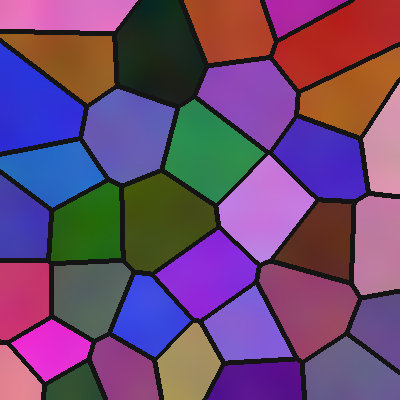
\includegraphics[width=36mm]{assets/drawn/grain-map}};
  \draw[white,line width=0.6pt] (map.south west) rectangle (map.north east);
  \draw[white,line width=0.9pt,-{Stealth[length=2mm,width=1.6mm]}] (131.5,-50.5) -- (131.5,-57);
  % the plane: 36 x 22 mm, yield strength 340-1000 MPa, elongation 30-86 %
  \begin{scope}[shift={(113.5,-83)}]
    \draw[white,line width=0.7pt] (0,22) -- (0,0) -- (36,0);
    \begin{scope}[x=0.054545mm,y=0.392857mm,shift={(-340,-30)}]
      \drawfront[white!75!udsblue,line width=0.6pt,dash pattern=on 1.4pt off 1pt]
      \foreach \s/\e/\i in \alloydata
        \node[circle,fill=white!85!udsblue,inner sep=0pt,minimum size=1.1mm] at (\s,\e) {};
      \node[circle,fill=white,inner sep=0pt,minimum size=4.6mm] (star) at (790,64) {};
      \node[text=udsred,font=\footnotesize] at (star) {\faStar};
    \end{scope}
  \end{scope}
  \fill[udsred] (102,1) rectangle (103.6,-91);}

% \doiline: https://doi.org/ and the paper's DOI, as a link in the slides; in the speaker notes, whose
% thumbnails scale the slide but not its links, the same text without a link
\newcommand\audiencemode{hide notes}
\ifx\notesmode\audiencemode
  \newcommand\doiline{\href{https://doi.org/\paperdoi}{https://doi.org/\paperdoi}}
\else
  \newcommand\doiline{\textcolor{udsblue}{https://doi.org/\paperdoi}}
\fi

% ------------------------------------------------------------------ title
\begin{frame}[plain,noframenumbering]
% Drawn inside the frame rather than over the page, so the speaker notes' thumbnail shows it too.
% The picture's origin is the page's top-left corner: a plain frame's body starts 8 mm in and
% 2 mm down.
\vbox to 0pt{\vskip-2mm\hbox to 0pt{\hskip-8mm\begin{tikzpicture}[x=1mm,y=1mm]
  \useasboundingbox (0,0) rectangle (160,-90);
  \titlepanel
  \node[anchor=north west,inner sep=0pt] at (8,-8) {\includegraphics[width=30mm]{\udslogo}};
  % the text block grows upwards from the presenter's name, whose baseline stays 66.5 mm from the top,
  % at the same distance from the d3M block as in the Coding Agents talk; the citation and the DOI under
  % it form one block, and the red rule sits halfway between that block and the name
  \node[anchor=south west,inner sep=0pt,text width=90mm,align=left,
    execute at begin node={\hyphenpenalty=10000\exhyphenpenalty=10000}] at (8,-66.63) {%
    {\fontsize{16.5}{18}\selectfont\bfseries\color{udsblue}\inserttitle\par}\vskip2mm
    {\fontsize{12}{14.5}\selectfont\color{udsdark}\insertsubtitle\par}\vskip0.6mm
    {\fontsize{9}{11}\selectfont\doiline\par}\vskip1.25mm
    \textcolor{udsred}{\rule{14mm}{0.8pt}}\par\vskip3mm
    {\fontsize{11}{13}\selectfont\color{udsdark}\insertauthor\par}};
  \node[anchor=south west,inner sep=0pt] (d3m) at (8,-83) {
\includegraphics[width=10mm]{assets/d3m.png}};
  \node[anchor=west,inner sep=0pt,text width=74mm,align=left,font=\fontsize{7}{8.8}\selectfont,
    execute at begin node={\hyphenpenalty=10000}] at ([xshift=3mm]d3m.east) {%
    {\color{udsblue}\insertinstitute\par}
    {\color{udsgrey}\insertdate\par}};
\end{tikzpicture}\hss}\vss}
% a frame with no tall content drops out of the notes' thumbnail; this invisible strut keeps it
\par\rule{0pt}{80mm}
\note{\textbf{0:00--0:20}\par
    A paper from Nature Communications, published at the end of September 2026.\par
    The authors train generative models on electron backscatter diffraction (EBSD) maps of 25 variants of
      one alloy, and search them for microstructures that are both stronger and more ductile.\par
    I follow the paper's own story.}
\end{frame}

% ---------------------------------------------------------------- outline
\begin{frame}{Outline}
  % each section's title as on its divider, and the divider's question
  \small\renewcommand\arraystretch{1.4}\setlength\tabcolsep{4pt}
  \begin{tabularx}{\textwidth}{@{}>{\leavevmode\color{udsblue}\bfseries}p{4mm}>{\bfseries}p{42mm}X@{}}
    \toprule
    1 & The design problem   & Why ask a generative model for new microstructures?\\
    2 & Groundwork           & Which methods does the paper build on?\\
    3 & The method           & How are microstructures generated and steered toward properties?\\
    4 & The results          & What do the authors show?\\
    \bottomrule
  \end{tabularx}
  \note{\textbf{0:20--0:50}\par
    Four sections, each answering one question.\par
    Section 2 introduces the machine-learning methods the paper combines, with their origins, for anyone
      who has not followed that literature.\par
    Sections 3 and 4 present the paper as the authors tell it.}
\end{frame}

\section[Problem]{The design problem}
\sectionframe{01}{The design problem}{Why ask a generative model for new microstructures?}{\faBalanceScale}

% ------------------------------------------------------------ the trade-off
\begin{frame}[source={Liao et al.\ (2026), Nat.\ Commun.\ 17, 11232}]{Strength/ductility trade-off}
  \begin{tikzpicture}[x=1mm,y=1mm]
    \useasboundingbox (0,0) rectangle (144,-54);
    \begin{scope}[shift={(16,-42)}]
      \planeaxes{340}{1000}{28}{86}{124}{42}{400,500,...,1000}{30,40,...,80}
      \begin{scope}[plane]
        \drawfront[front]
        \drawalloys
        \draw[udsred,line width=1.1pt,-{Stealth[length=2.6mm,width=2mm]}] (640,55) -- (760,72);
        \node[anchor=west,inner sep=0pt,font=\footnotesize\bfseries,text=udsred] at (768,73.5)
          {goal: stronger and more ductile};
        % the two ends of the trade-off, each beside the axis it is close to
        \node[anchor=west,inner sep=0pt,font=\footnotesize\bfseries,text=udsdark] at (410,84) {ductile, but weak};
        \node[anchor=east,inner sep=0pt,font=\footnotesize\bfseries,text=udsdark] at (1000,41) {strong, but brittle};
        \node[anchor=west,label text] at (360,33) {25 alloys, one processing route each};
        \node[anchor=west,small label] (fl) at (600,40) {measured front};
        \draw[udsgreymid,line width=0.4pt] (fl.north east) -- (700.46,45);
      \end{scope}
    \end{scope}
    \node[axis label] at (78,-49.4) {yield strength (MPa)};
    \node[axis label,rotate=90] at (3,-21) {elongation (\%)};
  \end{tikzpicture}
  \note{\textbf{1:00--2:10}\par
    Each point is one alloy: Inconel 625, a nickel-based superalloy used for turbine discs, blades and
      combustors, processed in one of 25 ways.\par
    The alloys differ only in processing: hot rolling and annealing at different temperatures and
      times.\par
    Each was tensile-tested for its yield strength and its elongation to failure.\par
    The stronger variants stretch less: a strength--ductility trade-off; making a metal stronger
      usually makes it brittle, and making it ductile makes it weak.\par
    The dashed staircase is the front: no measured alloy beats a point on it in both properties.\par
    The goal is a microstructure above and to the right of the front.\par
    Such microstructures are usually found by experience and trial and error over processing
      routes; the paper asks a generative model to propose them.}
\end{frame}

% ------------------------------------------------------- failure case
\begin{frame}[source={Liao et al.\ (2026), Nat.\ Commun.\ 17, 11232, Fig.\ 2c (CC BY-NC-ND 4.0)}]
  {Classic pixelwise loss fails}
  \begin{tikzpicture}[x=1mm,y=1mm]
    \useasboundingbox (0,0) rectangle (144,-54);
    \figpart{32}{0}{2}{340}{770}{1897}{1268}{112}
    \node[anchor=east,label text,align=right] at (29,{\fpy{884}}) {real patches};
    \node[anchor=east,label text,align=right,text=udsred] (pl) at (29,{\fpy{1155}}) {pixel loss only};
    % the two classic pixel losses over the n pixels of a patch x and its reconstruction
    \node[anchor=north east,inner sep=0pt,font=\scriptsize,text=udsdark,align=right] at ([yshift=-1.6mm]pl.south east)
      {MAE $=\frac{1}{n}\sum_i|x_i-\hat{x}_i|$\\[1.2mm] MSE $=\frac{1}{n}\sum_i(x_i-\hat{x}_i)^2$};
    \warnstrip{-41.4}{blurred or missing grain boundaries, colours mixed inside grains}
  \end{tikzpicture}
  \note{\textbf{2:10--3:10}\par
    These are real patches of 50 by 50 micrometres from test alloys, cut from EBSD maps.\par
    In an EBSD map each pixel's colour encodes the crystal orientation there: the three Euler angles
      as red, green and blue; the black lines are grain boundaries.\par
    The second row is what the paper's generator returns when it is trained to reproduce its input
      with a pixel loss alone, the mean absolute difference of the pixel values (MAE); the mean squared
      difference (MSE) is the other classic choice, and both average over all pixels.\par
    The boundaries blur, and colours mix inside grains, although a real grain has nearly one
      orientation.\par
    Boundaries cover few pixels, so an average over all pixels barely notices them; yet boundaries
      and orientations are what set the mechanical properties.}
\end{frame}

% ------------------------------------------------------------- the idea
\begin{frame}[source={Liao et al.\ (2026), Nat.\ Commun.\ 17, 11232, after Figs.\ 1 and 4f}]{Two fixes}
  \begin{tikzpicture}[x=1mm,y=1mm]
    \useasboundingbox (0,0) rectangle (144,-54);
    \tikzset{verdict mark/.style={circle,text=white,inner sep=0pt,minimum size=3.8mm,font=\scriptsize},
      head/.style={anchor=west,inner sep=0pt,font=\footnotesize\bfseries},
      panel title/.style={anchor=north west,inner sep=0pt,font=\footnotesize\bfseries,text=udsdark},
      note/.style={anchor=north west,label text,text width=22mm}}
    % column heads: what goes wrong, and what the paper changes
    \node[verdict mark,fill=udsred] (bad) at (1.9,-1.9) {\faTimes};
    \node[head,text=udsred] at ([xshift=1.6mm]bad.east) {the obstacle};
    \node[verdict mark,fill=testgreen] (good) at (87.9,-1.9) {\faCheck};
    \node[head,text=testgreen] at ([xshift=1.6mm]good.east) {the paper's fix};
    % row 1, the loss: the same patch region, three times enlarged, before and after
    \fill[redtint] (0,-5.6) rectangle (58,-28.4);
    \fill[greentint] (86,-5.6) rectangle (144,-28.4);
    \node[panel title] at (2.4,-7.4) {$L=L_{\mathrm{pix}}$};
    \node[panel title] at (88.4,-7.4) {$L=L_{\mathrm{pix}}+\textcolor{testgreen}{L_{\mathrm{edge}}+L_{\mathrm{SSIM}}}$};
    \foreach \x/\img in {2.4/grain-map-blurred,88.4/grain-map} {
      \node[anchor=north west,inner sep=0pt] at (\x,-12.6) {\includegraphics[width=14mm]{assets/drawn/\img}};
      \draw[udsdark,line width=0.4pt] ({\x+4.9},-17.5) rectangle ++(4.2,-4.2);
      \begin{scope}
        \clip ({\x+24},-19.6) circle (6.3);
        \node[anchor=north west,inner sep=0pt] at ({\x+3},1.4) {\includegraphics[width=42mm]{assets/drawn/\img}};
      \end{scope}
      \draw[udsdark,line width=0.5pt] ({\x+24},-19.6) circle (6.3);
      \draw[udsdark,line width=0.3pt] ({\x+9.1},-17.5) -- ({\x+19.6},-15.1) ({\x+9.1},-21.7) -- ({\x+19.6},-24.1);}
    \node[note] at (121.4,-13.4) {sharp boundaries, one colour per grain};
    \fixarrow{60.4}{83.6}{-17}{more terms}
    % row 2, the sampling: the latent space sampled at random, and searched toward targets (after Fig. 1c)
    \fill[redtint] (0,-31.2) rectangle (58,-54);
    \fill[greentint] (86,-31.2) rectangle (144,-54);
    \node[panel title] at (2.4,-33) {random sampling};
    \node[panel title] at (88.4,-33) {property-guided search};
    \tikzset{code/.style={circle,fill=udsgreymid,inner sep=0pt,minimum size=1.3mm},
      new code/.style={circle,fill=udsblue,inner sep=0pt,minimum size=1.5mm},
      latent/.style={fill=white,draw=udsgreylight,line width=0.4pt}}
    % left: codes drawn at random fall among the training codes
    \filldraw[latent] (14,-43.6) ellipse (10 and 7);
    \foreach \x/\y in {9.6/-38.6,7/-41.4,5.8/-43.8,8.4/-45,9.8/-48.4,14.6/-38.4,19.6/-39,18.6/-48.2,14.8/-49.2}
      \node[code] at (\x,\y) {};
    \node[anchor=north,small label] at (14,-51.2) {latent space};
    % the three new codes join, and one arrow goes on to the sentence about them; the training codes
    % leave each line a clear path
    \node[note,text width=27mm,anchor=west] at (28.4,-43.6) {new codes fall among the training codes};
    \foreach \x/\y in {12/-40.4,15.8/-43.6,11.2/-47}
      \draw[udsblue,line width=0.5pt,shorten <=1mm] (\x,\y) to[out=0,in=180] (22.4,-43.6);
    \draw[udsblue,line width=0.5pt,-{Stealth[length=1.5mm,width=1.1mm]}] (22.4,-43.6) -- (27.4,-43.6);
    \foreach \x/\y in {12/-40.4,15.8/-43.6,11.2/-47} \node[new code] at (\x,\y) {};
    % right: the search steers codes to targets outside them, beyond the measured front (after Fig. 1c)
    \filldraw[latent] (97.6,-45) ellipse (8 and 5.8);
    \foreach \x/\y in {-4.6/1.4,-2/-2.4,0.4/2.6,2.2/-0.6,4.6/1.6,-0.6/-4,5/-2.6,-5.4/-1.2}
      \node[code] at (97.6+\x,-45+\y) {};
    \draw[udsblue,line width=0.9pt,-{Stealth[length=1.8mm,width=1.4mm]}] (104.8,-42.6) -- (107.9,-41.4);
    \filldraw[fill=udsblue!22,draw=udsblue,line width=0.4pt] (111.2,-40.6) circle (3.2);
    \foreach \x/\y in {-1.2/0.9,1.2/-0.9} \node[text=udsred,font=\tiny] at (111.2+\x,-40.6+\y) {\faStar};
    \node[anchor=north,small label] at (97.6,-51.2) {latent space};
    \node[anchor=north,small label] at (111.2,-44.2) {targets};
    \begin{scope}[shift={(119,-49.4)}]
      \draw[udsgreymid,line width=0.5pt] (0,11.4) -- (0,0) -- (22,0);
      \node[anchor=north,small label] at (11,-0.6) {strength};
      \node[anchor=south,small label,rotate=90] at (-0.6,5.7) {elongation};
      \begin{scope}[x=0.033333mm,y=0.203571mm,shift={(-340,-30)}]
        \drawfront[front]
        \drawalloys[minimum size=1mm]
        \draw[udsred,line width=0.7pt,-{Stealth[length=1.6mm,width=1.2mm]}] (600,51) -- (660,61);
        \drawcandidates[minimum size=1.3mm]
      \end{scope}
    \end{scope}
    \fixarrow{60.4}{83.6}{-42.2}{steer by properties}
  \end{tikzpicture}
  \note{\textbf{3:10--4:10}\par
    The paper answers two obstacles with two changes: the obstacles on the left, its fixes on the
      right.\par
    First, a pixel loss alone blurs grain boundaries, as the enlarged region shows; the paper adds two
      terms, one that responds to grain boundaries and one to the structure inside grains.\par
    Second, codes drawn at random from the model's latent space fall among the training codes, so the new
      samples resemble the measured alloys.\par
    So the authors search the latent space, steered by predicted strength and ductility, toward targets
      outside the training codes, as their Fig.~1c sketches; their five candidates lie beyond the measured
      front.\par
    Section 2 explains the models and the search for anyone who has not met them.}
\end{frame}

\section[Groundwork]{Groundwork}
\sectionframe{02}{Groundwork}{Which methods does the paper build on?}{\faBookOpen}

% ----------------------------------------------------- three ways to generate
\begin{frame}[source={Kingma and Welling (2013), arXiv:1312.6114 · Goodfellow et al.\ (2014), NeurIPS · Ramesh et al.\ (2021), ICML · Ho et al.\ (2020), NeurIPS · Rombach et al.\ (2022), CVPR}]
  {Three ways to generate an image}
  \begin{tikzpicture}[x=1mm,y=1mm]
    \useasboundingbox (0,0) rectangle (144,-54);
    \foreach \i/\c/\h in {0/udsblue/In one pass,1/udsgreymid/Token by token,2/udsblue/Step by step from noise} {
      \pgfmathsetmacro\cx{\i*49}
      \fill[\c!8] (\cx,-5.4) rectangle ++(46,-41.6);
      \cardhead{\cx}{0}{46}{\c}{\h}
    }
    % in one pass: a code, decoded into the whole image
    \filldraw[fill=udsblue,draw=udsblue] (6,-12.3) rectangle (10.4,-19.7);
    \node[text=white,font=\small\itshape,inner sep=0pt] at (8.2,-16) {z};
    \draw[flow] (11,-16) -- (14.2,-16);
    \filldraw[fill=bluetint,draw=udsblue,line width=0.5pt] (15,-12.5) -- (25.4,-9) -- (25.4,-23) -- (15,-19.5) -- cycle;
    \node[label text,rotate=90] at (20.2,-16) {decoder};
    \draw[flow] (26,-16) -- (29.2,-16);
    \node[anchor=north west,inner sep=0pt] at (30,-9.5) {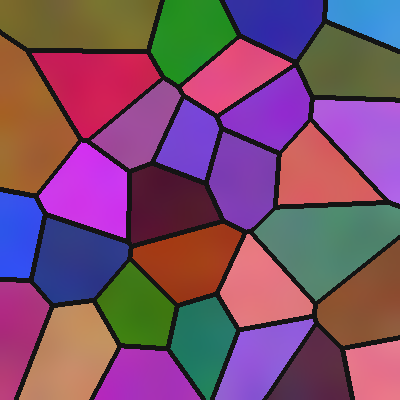
\includegraphics[width=13mm]{assets/drawn/grain-map-new}};
    % token by token: tiles written in reading order, the next one outlined
    \node[anchor=north west,inner sep=0pt] at (65,-9) {
\includegraphics[width=14mm]{assets/drawn/tokens-partial}};
    \begin{scope}[shift={(65,-23)}]
      \draw[udsgreylight,line width=0.3pt] (0,0) grid[step=1.75] (14,14);
      \draw[udsred,line width=0.8pt] (5.25,7) rectangle (7,8.75);
    \end{scope}
    % step by step from noise: the whole image refined at every step
    \foreach \t/\x in {1000/100.5,150/116,0/131.5}
      \node[anchor=north west,inner sep=0pt] at (\x,-10.5) {\includegraphics[width=11mm]{assets/drawn/diffusion-t\t}};
    \draw[flow,draw=udsblue] (112,-16) -- (115.4,-16);
    \draw[flow,draw=udsblue] (127.5,-16) -- (130.9,-16);
    % what each does, examples, and how the image is built
    \foreach \i/\a/\e/\b in {0/{a decoder turns a code into an image}/{VAE (2013), GAN (2014)}/{whole image at once},
        1/{a network predicts each tile from the tiles before it}/{DALL-E 1 (2021); language models write text
          this way}/{no going back to refine},
        2/{a network removes a little noise at each step}/{DDPM (2020), Stable Diffusion (2022), DALL-E 2
          (2022)}/{refines the whole image}} {
      \node[card text,text width=42mm] at ({\i*49+2},-26.6) {\a};
      \node[card text,text width=42mm,font=\scriptsize,text=udsgrey] at ({\i*49+2},-35) {\e};
      \node[card text,text width=42mm,font=\footnotesize\bfseries] at ({\i*49+2},-42.4) {\b};}
    \node[anchor=north west,small label,text=udsred] at (0,-49.4)
      {Liao et al.\ join the first and the third: the VAE output guides the diffusion steps};
  \end{tikzpicture}
  \note{\textbf{4:20--5:20}\par
    Generative models differ in how they build an image.\par
    In one pass: a decoder turns a short code into the whole image at once; VAEs and GANs work this
      way.\par
    Token by token: a network predicts each piece of the image from the pieces before it, as language
      models write text word by word; DALL-E 1 (Ramesh and colleagues, 2021) wrote 32 by 32 such tokens,
      which a discrete VAE then decoded into the image.\par
    Such a model starts from scratch and works in a fixed order, so it cannot go back and refine what it
      has written.\par
    Step by step from noise: a diffusion model starts from noise and refines the whole image at every
      step; Stable Diffusion and DALL-E 2 and 3 work this way, and diffusion leads image generation
      today.\par
    The paper joins the first and the third: a VAE generates in one pass, and its output guides the
      diffusion steps.}
\end{frame}

% ------------------------------------------------------------------ VAE
\begin{frame}[source={Kingma and Welling (2013), arXiv:1312.6114}]{Variational Autoencoder (VAE)}
  \begin{tikzpicture}[x=1mm,y=1mm]
    \useasboundingbox (0,0) rectangle (144,-54);
    \tikzset{part/.style={fill=bluetint,draw=udsblue,line width=0.5pt}}
    % encode, sample, decode; the row's centre line is y = -11.5
    \node[anchor=north west,inner sep=0pt] at (0,-5.5) {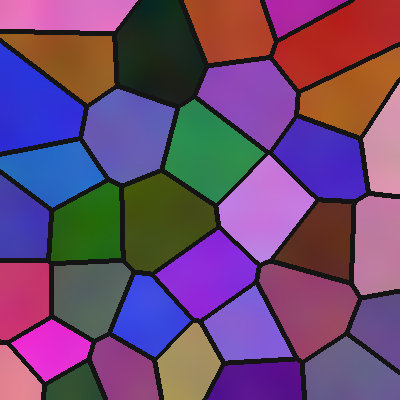
\includegraphics[width=12mm]{assets/drawn/grain-map}};
    \node[anchor=north,small label,text=udsdark] at (6,-18.4) {patch};
    \draw[flow] (12.6,-11.5) -- (16.6,-11.5);
    \filldraw[part] (17.4,-4) -- (27.8,-7.5) -- (27.8,-15.5) -- (17.4,-19) -- cycle;
    \node[label text,rotate=90] at (22.6,-11.5) {encoder};
    \draw[flow] (28.4,-11.5) -- (31.4,-11.5);
    \filldraw[fill=bluetint,draw=udsblue,line width=0.5pt] (32,-6.8) rectangle (36,-11.1);
    \filldraw[fill=darktint,draw=udsdark,line width=0.5pt] (32,-11.9) rectangle (36,-16.2);
    \node[font=\scriptsize,inner sep=0pt,text=udsdark] at (34,-8.95) {$\mu$};
    \node[font=\scriptsize,inner sep=0pt,text=udsdark] at (34,-14.05) {$\sigma$};
    \node[anchor=north,small label,text=udsdark,align=center] at (34,-18.4) {mean,\\ spread};
    \draw[flow] (36.6,-11.5) -- (39.6,-11.5);
    % sample: a normal curve with one drawn value
    \draw[udsgreymid,line width=0.4pt] (40.4,-14.5) -- (49.6,-14.5);
    \draw[udsblue,line width=0.7pt] plot[domain=-2.6:2.6,samples=41] ({45+\x*1.75},{-14.5+6.5*exp(-((\x)^2)/2)});
    \node[circle,fill=udsred,inner sep=0pt,minimum size=1.5mm] at (46.6,-14.5) {};
    \node[anchor=north,small label,text=udsdark] at (45,-18.4) {sample $z$};
    \draw[flow] (50.2,-11.5) -- (53.2,-11.5);
    \filldraw[part] (54,-7.5) -- (64.4,-4) -- (64.4,-19) -- (54,-15.5) -- cycle;
    \node[label text,rotate=90] at (59.2,-11.5) {decoder};
    \draw[flow] (65,-11.5) -- (69,-11.5);
    \node[anchor=north west,inner sep=0pt] at (69.6,-5.5) {
\includegraphics[width=12mm]{assets/drawn/grain-map-blurred}};
    \node[anchor=north,small label,text=udsdark] at (75.6,-18.4) {reconstruction};
    % the loss, each term labelled
    \node[font=\large,text=udsdark,inner sep=0pt] at (4,-32) {$L\;=$};
    \node[font=\large,text=udsdark,inner sep=0pt] (rec) at (21,-32) {$L_{\mathrm{rec}}$};
    \node[font=\large,text=udsdark,inner sep=0pt] at (41,-32) {$+$};
    \node[font=\large,text=udsblue,inner sep=0pt] (kl) at (62,-32) {$L_{\mathrm{KL}}$};
    \node[anchor=north,label text,align=center,text width=28mm] at (21,-36.4) {output close\\ to the input};
    \node[anchor=north,label text,align=center,text width=28mm,text=udsblue] at (62,-36.4)
      {codes close to\\ a standard normal};
    % the latent space: each patch's code is a small cloud, and the clouds overlap
    \draw[udsgreymid,line width=0.5pt] (92,0) rectangle (144,-44);
    \node[anchor=north west,small label] at (93.4,-1.4) {latent space, 2 of 128 directions};
    \foreach \x/\y in {104/-24,110/-18,111/-29,117/-23,103/-33,118/-33,124/-27,109/-38,98/-28}
      {\fill[udsblue,fill opacity=0.14] (\x,\y) circle (4.4); \fill[udsblue] (\x,\y) circle (0.55);}
    \node[text=udsred,font=\footnotesize,inner sep=0pt] (new) at (114.2,-24.4) {\faStar};
    \node[anchor=north west,inner sep=0pt] (np) at (129.4,-9.4) {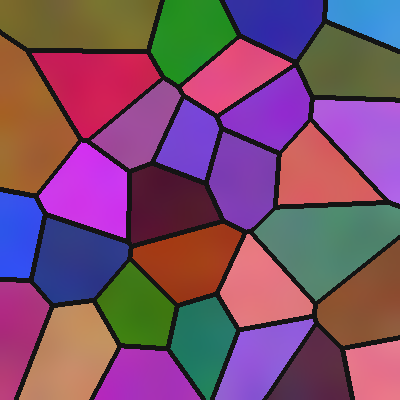
\includegraphics[width=11mm]{assets/drawn/grain-map-new}};
    \draw[udsred,line width=0.7pt,-{Stealth[length=1.6mm,width=1.2mm]}] (new.north east) to[out=40,in=200] (np.west);
    \node[anchor=north,small label,text=udsred,align=center] at (134.9,-21.2) {new code,\\ new patch};
  \end{tikzpicture}
  \note{\textbf{5:20--6:40}\par
    An autoencoder is a network trained to copy its input through a bottleneck: an encoder compresses the
      image into a few numbers, the latent code, and a decoder rebuilds the image from them.\par
    The variational autoencoder, from Kingma and Welling in 2013, makes the code probabilistic: the
      encoder gives a mean and a spread for each number, and the decoder sees a value drawn from that
      range.\par
    A Kullback--Leibler (KL) term pulls every code towards a standard normal distribution, so the codes
      of different images overlap and the space has no gaps.\par
    That makes a VAE generative: a code drawn from this space decodes to a plausible image, and moving
      through the space changes the image smoothly.\par
    Trained with a pixel loss, a VAE returns blurry images, the average of the plausible answers: the
      failure of slide 3.\par
    In this paper each patch gets a code of 128 numbers.}
\end{frame}

% ----------------------------------------------- reconstruct, generate, extrapolate
\begin{frame}{Reconstruct, generate, extrapolate}
  \begin{tikzpicture}[x=1mm,y=1mm]
    \useasboundingbox (0,0) rectangle (144,-54);
    \tikzset{code/.style={circle,fill=udsgreymid,inner sep=0pt,minimum size=1.2mm}}
    \foreach \i/\c/\h in {0/udsdark/Reconstruct,1/udsblue/Generate,2/udsred/Extrapolate} {
      \pgfmathsetmacro\cx{\i*49}
      \fill[\c!8] (\cx,-5.4) rectangle ++(46,-41.6);
      \cardhead{\cx}{0}{46}{\c}{\h}
      % the training codes, the same cloud in every card
      \begin{scope}[shift={(\cx,0)}]
        \filldraw[fill=white,draw=udsgreylight,line width=0.5pt] (21,-16.5) ellipse (8.6 and 5.6);
        \foreach \x/\y in {16/-15,18.6/-19,20.4/-13.6,22.6/-17.4,24.8/-14.6,26.2/-18.4,15.4/-17.8,19.4/-16.2}
          \node[code] at (\x,\y) {};
      \end{scope}
    }
    % reconstruct: a training patch, encoded and decoded
    \node[anchor=north west,inner sep=0pt] (in) at (1.4,-11.5) {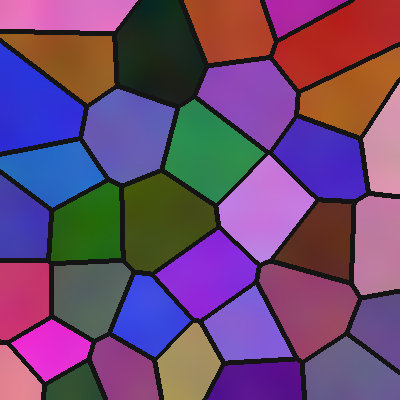
\includegraphics[width=10mm]{assets/drawn/grain-map}};
    \node[circle,draw=udsdark,line width=0.7pt,inner sep=0pt,minimum size=2.6mm] (c0) at (22.6,-17.4) {};
    \draw[flow,line width=0.5pt] (in.east) to[out=0,in=180] (c0.west);
    \node[anchor=north west,inner sep=0pt] (out0) at (34.6,-11.5) {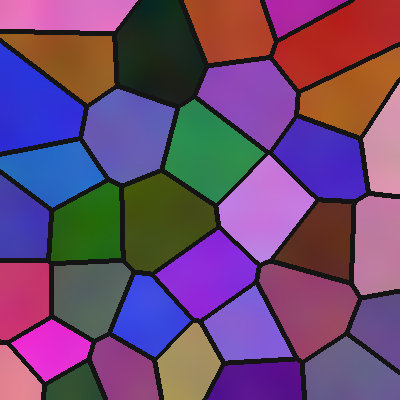
\includegraphics[width=10mm]{assets/drawn/grain-map}};
    \draw[flow,line width=0.5pt] (c0.east) to[out=0,in=180] (out0.west);
    % generate: a new code among the training codes
    \node[circle,fill=udsblue,inner sep=0pt,minimum size=2mm] (c1) at (49+23.4,-15.6) {};
    \node[anchor=north west,inner sep=0pt] (out1) at (49+34.6,-11.5) {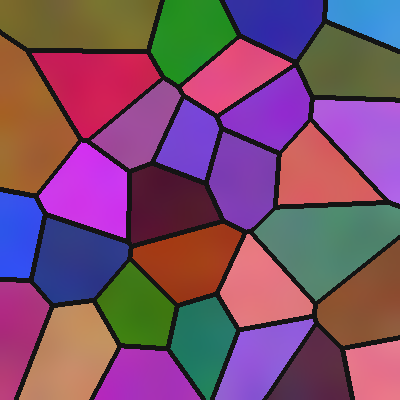
\includegraphics[width=10mm]{assets/drawn/grain-map-new}};
    \draw[flow,draw=udsblue,line width=0.5pt] (c1.east) to[out=0,in=180] (out1.west);
    % extrapolate: a code away from every training code
    \node[text=udsred,font=\footnotesize,inner sep=0pt] (c2) at (98+31.4,-25.4) {\faStar};
    \node[anchor=north west,inner sep=0pt] (out2) at (98+34.6,-11.5) {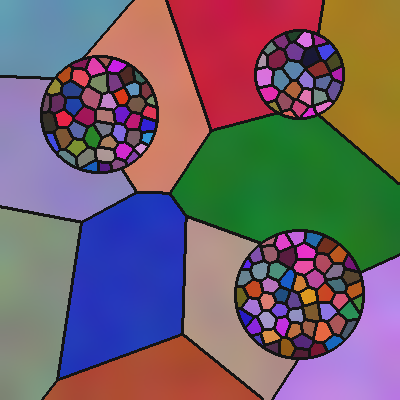
\includegraphics[width=10mm]{assets/drawn/grain-map-bimodal}};
    \node[circle,fill=white,draw=udsred,line width=0.6pt,inner sep=0pt,minimum size=4.2mm,font=\scriptsize\bfseries,
      text=udsred] at ([xshift=-1mm,yshift=1mm]out2.north east) {?};
    \draw[flow,draw=udsred,line width=0.5pt] (c2.east) to[out=0,in=-90] (out2.south);
    % what each is, and what can check it
    \foreach \i/\a/\b in {0/{a training patch, encoded and decoded}/{compare with its input},
        1/{a new code among the training codes}/{compare with held-out data},
        2/{a code away from all training codes}/{only an experiment can tell}} {
      \node[anchor=north west,card text,text width=42mm] at ({\i*49+2},-29.4) {\a};
      \node[anchor=north west,card text,text width=42mm,font=\footnotesize\bfseries] at ({\i*49+2},-41.4) {\b};}
  \end{tikzpicture}
  \note{\textbf{6:40--7:40}\par
    A trained generative model can do three different things, and each needs a different check.\par
    Reconstruct: encode a training patch and decode it again; the result can be compared with its own
      input, pixel by pixel or by its statistics.\par
    Generate: decode a new code from among the training codes; the result has no original, so it is
      compared with the statistics of held-out data and checked for near-copies of training patches.\par
    Extrapolate: decode a code away from all training codes; no example lies there, so only an
      experiment can tell whether the result is realistic.\par
    The paper claims all three; the results show what each claim rests on.}
\end{frame}

% ------------------------------------------------------------ diffusion
\begin{frame}[source={Sohl-Dickstein et al.\ (2015), ICML · Ho et al.\ (2020), NeurIPS · Ronneberger et al.\ (2015), MICCAI}]
  {Diffusion models}
  \begin{tikzpicture}[x=1mm,y=1mm]
    \useasboundingbox (0,0) rectangle (144,-54);
    \node[anchor=north west,label text,text=udsgrey] (fwd) at (0,0)
      {forward: at each of 1000 steps, mix in a little noise\enspace\textcolor{udsgreymid}{(fixed)}};
    \node[anchor=base east,label text] at (fwd.base -| 144,0) {$x_t=\sqrt{1-\beta_t}\,x_{t-1}+\sqrt{\beta_t}\,\epsilon$};
    \foreach \t [count=\i from 0] in {0,50,150,300,1000} {
      \node[anchor=north west,inner sep=0pt] (d\i) at ({2+29*\i},-6.6) {\includegraphics[width=18mm]{assets/drawn/diffusion-t\t}};
      \node[anchor=north,small label,text=udsdark] at ({11+29*\i},-25.4) {$t=\t$};}
    \foreach \i in {0,...,3} {
      \draw[flow,draw=udsgreymid] ({20.6+29*\i},-11.6) -- ({30.4+29*\i},-11.6);
      \draw[flow,draw=udsblue] ({30.4+29*\i},-19.6) -- ({20.6+29*\i},-19.6);}
    \node[anchor=north west,label text,text=udsblue] at (0,-30.4)
      {reverse: a U-Net predicts the noise, removed step by step\enspace\textcolor{udsblue!70}{(learned)}};
    % generating with the trained model, two ways: from noise alone, or from noise and a guide (the paper)
    \tikzset{step image/.style={anchor=west,inner sep=0pt},
      way name/.style={anchor=west,inner sep=0pt,font=\footnotesize\bfseries,text=udsdark},
      way text/.style={card text,anchor=west,text width=84mm}}
    \node[anchor=north west,label text,text=udsgrey] at (0,-34.4) {generating with the trained model, two ways:};
    \foreach \y in {-41.6,-49.8} \fill[bluetint] (0,\y+3.9) rectangle (144,\y-3.9);
    % unconditional: noise alone
    \node[way name] at (2.4,-41.6) {unconditional};
    \node[step image] (u0) at (27,-41.6) {
\includegraphics[width=6.6mm]{assets/drawn/diffusion-t1000}};
    \node[step image] (u1) at (49.4,-41.6) {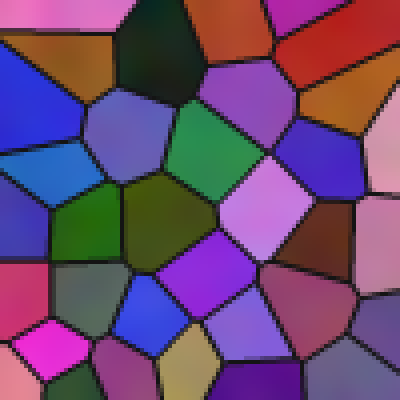
\includegraphics[width=6.6mm]{assets/drawn/diffusion-t0}};
    \draw[flow,draw=udsblue] ([xshift=0.6mm]u0.east) -- ([xshift=-0.6mm]u1.west);
    \node[way text] at (59,-41.6) {from noise alone, step by step: a new patch of any kind};
    % conditional: noise and a guide image
    \node[way name] at (2.4,-49.8) {conditional};
    \node[step image] (c0) at (27,-49.8) {
\includegraphics[width=6.6mm]{assets/drawn/diffusion-t1000}};
    \node[font=\small\bfseries,text=udsdark,inner sep=0pt] at (35.4,-49.8) {+};
    \node[step image] (c1) at (37.2,-49.8) {
\includegraphics[width=6.6mm]{assets/drawn/grain-map-blurred}};
    \draw[udsred,line width=0.6pt] (c1.south west) rectangle (c1.north east);
    \node[step image] (c2) at (49.4,-49.8) {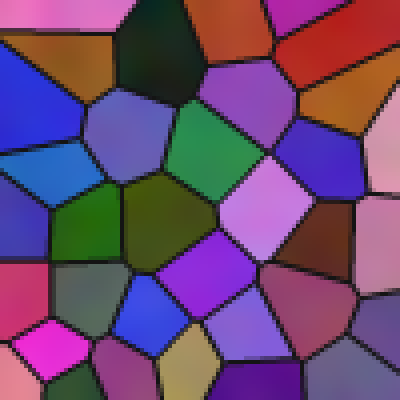
\includegraphics[width=6.6mm]{assets/drawn/diffusion-t0}};
    \draw[flow,draw=udsblue] ([xshift=0.6mm]c1.east) -- ([xshift=-0.6mm]c2.west);
    \node[way text] at (59,-49.8) {the U-Net also sees a \textcolor{udsred}{guide} at every step, here the VAE
      output};
  \end{tikzpicture}
  \note{\textbf{7:40--8:50}\par
    A diffusion model learns to undo noise.\par
    The forward process is fixed: each of 1000 steps scales the image down slightly and adds a little
      Gaussian noise $\epsilon$, with $\beta_t$ rising from 0.0001 to 0.02; after a few hundred steps only
      noise is left.\par
    Each step depends only on the one before, a Markov chain; the paper writes it as a Gaussian, its
      Eq.~12.\par
    The reverse process is learned: a network predicts the noise in an image at any step, and removing it
      step by step runs the process backwards.\par
    The idea is from Sohl-Dickstein and colleagues, 2015; DDPM, from Ho, Jain and Abbeel in 2020, made
      the images sharp.\par
    Once trained, it generates in two ways: from noise alone, any new patch; or with a guide image that
      the U-Net sees at every step, a patch that follows the guide.\par
    The paper's guide is the VAE's blurry output, so the diffusion model only restores detail; the next
      slide shows the training.}
\end{frame}

% ---------------------------------------------------- training a diffusion model
\begin{frame}[source={Ho et al.\ (2020), NeurIPS · Ronneberger et al.\ (2015), MICCAI}]
  {Training a diffusion model}
  \begin{tikzpicture}[x=1mm,y=1mm]
    \useasboundingbox (0,0) rectangle (144,-54);
    \begin{scope}[yshift=1mm]% content starts 4 mm below the title
    % a patch and a noise image, mixed in one go to a random step t
    \node[anchor=north west,inner sep=0pt] (x0) at (0,-1) {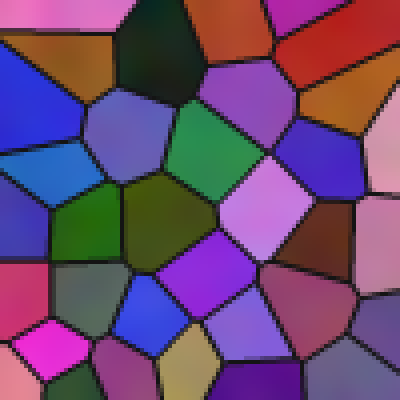
\includegraphics[width=12mm]{assets/drawn/diffusion-t0}};
    \node[anchor=north,small label,text=udsdark] at (6,-13.8) {patch $x_0$};
    \node[anchor=north west,inner sep=0pt] (eps) at (0,-21) {
\includegraphics[width=12mm]{assets/drawn/diffusion-noise}};
    \node[anchor=north,small label,text=udsdark] at (6,-33.8) {noise $\epsilon$};
    \node[draw=udsgreymid,fill=darktint,line width=0.5pt,inner sep=1.6mm,align=center,font=\footnotesize,
      text=udsdark] (mix) at (39,-7)
      {{\scriptsize\color{udsgrey}a random step $t$, in one go}\\[0.6mm]
       $x_t=\sqrt{\bar\alpha_t}\,x_0+\sqrt{1-\bar\alpha_t}\,\epsilon$};
    \draw[flow] (x0.east) -- (x0.east -| mix.west);
    \draw[flow] (12,-24) to[out=0,in=-90] (30,-12.6 |- mix.south);
    % the noised patch and its step go into the U-Net, which predicts the noise
    \node[anchor=north west,inner sep=0pt] (xt) at (66,-1) {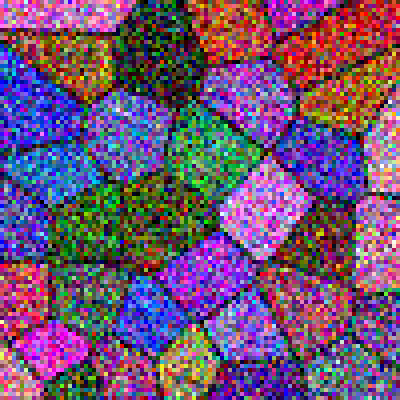
\includegraphics[width=12mm]{assets/drawn/diffusion-t150}};
    \node[anchor=north,small label,text=udsdark] at (72,-13.8) {$x_t$, here $t=150$};
    \draw[flow] (mix.east) -- (mix.east -| xt.west);
    \node[draw=udsblue,fill=bluetint,line width=0.5pt,minimum width=14mm,minimum height=9mm,font=\footnotesize,
      text=udsblue,inner sep=0pt] (unet) at (92,-7) {U-Net};
    \draw[flow] (xt.east |- unet.west) -- (unet.west);
    \node[anchor=north,small label,text=udsdark] (tin) at (92,-17.4) {step $t$};
    \draw[flow,line width=0.5pt] (tin.north) -- (unet.south);
    \node[anchor=west,font=\footnotesize,text=udsblue,inner sep=0pt] (pred) at (105.2,-7) {$\epsilon_\theta(x_t,t)$};
    \node[anchor=north,small label,text=udsblue] at ([yshift=-1.4mm]pred.south) {predicted noise};
    \draw[flow] (unet.east) -- (pred.west);
    % the loss: the predicted noise against the noise that was added
    \node[draw=udsred,fill=redtint,line width=0.5pt,inner sep=1.6mm,font=\footnotesize,text=udsdark] (loss)
      at (pred.center |- 0,-29) {$\|\epsilon-\epsilon_\theta(x_t,t)\|^2$};
    \draw[flow] ([yshift=-5.6mm]pred.south) -- (loss.north);
    \draw[flow,draw=udsred] (eps.east |- loss.west) -- (loss.west);
    \node[anchor=south,small label,text=udsred] at (56,-28.4) {the noise that was added is the target};
    \node[anchor=west,small label,text width=14mm] at ([xshift=1.6mm]loss.east) {loss: trains the U-Net};
    \end{scope}
    % repeated over many patches; the paper adds the VAE output as an input
    \fill[bluetint] (0,-40.4) rectangle (70,-53.6);
    \node[card text,anchor=west,text width=66mm] at (2,-47) {repeated over many patches, steps and noise
      images: one U-Net learns all 1000 steps};
    \fill[redtint] (74,-40.4) rectangle (144,-53.6);
    \node[card text,anchor=west,text width=66mm] at (76,-47) {Liao et al.: the U-Net also sees the VAE output,
      $\epsilon_\theta(x_t,t,x_V)$};
  \end{tikzpicture}
  \note{\textbf{8:50--10:00}\par
    A diffusion model is trained on one simple task: predict the noise in a noised image.\par
    Take a training patch $x_0$, draw a noise image $\epsilon$ and a random step $t$, and mix them in one
      go; $\bar\alpha_t$, the product of all $1-\beta_s$ up to step $t$, says how much of the patch is
      left.\par
    The network, a U-Net (Ronneberger and colleagues, 2015), gets the noised patch and the step and returns
      a noise image of the same size.\par
    The loss is the squared error between the added and the predicted noise; repeated over many patches,
      steps and noise images, one network learns every step.\par
    Knowing the noise is enough to step back: each reverse step subtracts a share of the predicted noise
      and adds a little fresh noise.\par
    The paper trains its diffusion model this way, with the VAE output $x_V$ as a third input, and
      compares the noise with the loss of section 3.}
\end{frame}

% --------------------------------------------------------- Pareto, NSGA-II
\begin{frame}[source={Pareto (1906), \emph{Manuale di economia politica} · Holland (1975), \emph{Adaptation in Natural and Artificial Systems} · Deb et al.\ (2002), IEEE Trans.\ Evol.\ Comput.\ 6, 182}]
  {Pareto fronts and NSGA-II}
  \begin{tikzpicture}[x=1mm,y=1mm]
    \useasboundingbox (0,0) rectangle (144,-54);
    \tikzset{panel frame/.style={draw=udsgreylight,line width=0.5pt,rounded corners=1mm},
      name part/.style={anchor=north,inner sep=0pt,font=\Large\bfseries,text=udsblue},
      name meaning/.style={anchor=north,small label,text=udsdark},
      front point/.style={circle,fill=udsblue,inner sep=0pt,minimum size=1.6mm},
      back point/.style={circle,fill=udsgreymid,inner sep=0pt,minimum size=1.6mm},
      point name/.style={inner sep=0pt,font=\scriptsize\bfseries,text=udsdark},
      ga row/.style={anchor=west,label text},
      ga icon/.style={font=\footnotesize,text=udsblue}}
    % the name, part by part, over the panel that explains each part
    \foreach \x/\l/\m in {22/NS/non-dominated sorting,72/GA/genetic algorithm,122/II/crowding distance} {
      \node[name part] at (\x,0) {\l};
      \node[name meaning] at (\x,-5.2) {\m};}
    \foreach \x in {0,50,100} \draw[panel frame] (\x,-9.2) rectangle ++(44,-38.4);
    % NS: A beats B in both goals; nobody beats A, C or D in both, so they form front 1
    \begin{scope}[shift={(5,-43.6)}]
      \draw[udsgreymid,line width=0.5pt,-{Stealth[length=1.4mm,width=1mm]}] (0,0) -- (38,0);
      \draw[udsgreymid,line width=0.5pt,-{Stealth[length=1.4mm,width=1mm]}] (0,0) -- (0,30.4);
      \node[anchor=north east,small label] at (38,-0.6) {goal 1};
      \node[anchor=south east,small label,rotate=90] at (-0.6,30.4) {goal 2};
      \begin{scope}[x=36mm,y=29mm]
        \fill[redtint] (0,0) rectangle (0.8,0.8);
        \node[anchor=south west,small label,text=udsred] at (0.04,0.05) {A beats B in both};
        \draw[udsgreymid,line width=0.6pt,dash pattern=on 1.4pt off 1pt]
          (0.35,0.75) -- (0.35,0.6) -- (0.6,0.6) -- (0.6,0.4) -- (0.7,0.4);
        \draw[udsblue,line width=0.8pt] (0.5,0.95) -- (0.5,0.8) -- (0.8,0.8) -- (0.8,0.5) -- (0.95,0.5);
        \foreach \u/\v in {0.5/0.95,0.8/0.8,0.95/0.5} \node[front point] at (\u,\v) {};
        \foreach \u/\v in {0.35/0.75,0.6/0.6,0.7/0.4} \node[back point] at (\u,\v) {};
        \foreach \n/\u/\v/\dx/\dy/\a in {A/0.8/0.8/0.9/0.9/south west,B/0.6/0.6/0.9/0.9/south west,
            C/0.95/0.5/0/1.2/south,D/0.5/0.95/-1.2/0/east}
          \node[point name,anchor=\a] at ([shift={(\dx mm,\dy mm)}]\u,\v) {\n};
        \node[anchor=west,small label,text=udsblue] at (0.56,0.97) {front 1};
        \node[anchor=north west,small label,text=udsgreymid] at (0.36,0.57) {front 2};
      \end{scope}
    \end{scope}
    % GA: one generation, top to bottom, and round again
    \foreach \y/\icon/\t in {-14.4/\faUsers/population,-22.4/\faBalanceScale/score both goals,
        -30.4/\faFilter/{keep the best: by front,\\ then by crowding},-38.4/\faRandom/{cross over, mutate}} {
      \node[ga icon] at (57.6,\y) {\icon};
      \node[ga row] at (62.4,\y) {\t};}
    \foreach \y in {-14.4,-22.4,-30.4} \draw[flow,draw=udsblue,line width=0.5pt] (57.6,\y-2.4) -- (57.6,\y-5.6);
    \draw[flow,draw=udsblue,line width=0.5pt] (55,-38.4) -- (52.6,-38.4) -- (52.6,-14.4) -- (55,-14.4);
    \node[anchor=north,small label,text=udsdark] at (71.5,-42.2) {repeat for hundreds of generations};
    % the two rules of "keep the best" come from the panels beside it
    \draw[flow,draw=udsblue] (44.6,-30.4) -- (49.4,-30.4);
    \draw[flow,draw=udsblue] (99.4,-30.4) -- (94.6,-30.4);
    % II: on a crowded front, near-copies are dropped and points with room around them kept
    \begin{scope}[shift={(105,-43.6)}]
      \draw[udsgreymid,line width=0.5pt,-{Stealth[length=1.4mm,width=1mm]}] (0,0) -- (38,0);
      \draw[udsgreymid,line width=0.5pt,-{Stealth[length=1.4mm,width=1mm]}] (0,0) -- (0,30.4);
      \node[anchor=north east,small label] at (38,-0.6) {goal 1};
      \node[anchor=south east,small label,rotate=90] at (-0.6,30.4) {goal 2};
      \begin{scope}[x=36mm,y=29mm]
        \draw[testgreen,line width=0.6pt,dash pattern=on 1.2pt off 0.8pt] (0.12,0.62) rectangle (0.76,0.95);
        \draw[udsblue,line width=0.8pt] (0.12,0.95) -- (0.12,0.85) -- (0.45,0.85) -- (0.45,0.62) -- (0.76,0.62)
          -- (0.76,0.6) -- (0.8,0.6) -- (0.8,0.58) -- (0.84,0.58) -- (0.84,0.3) -- (0.95,0.3);
        \foreach \u/\v in {0.12/0.95,0.45/0.85,0.76/0.62,0.8/0.6,0.84/0.58,0.95/0.3} \node[front point] at (\u,\v) {};
        \node[text=udsred,font=\footnotesize\bfseries,inner sep=0pt] at (0.8,0.6) {\faTimes};
        \node[anchor=south west,small label,text=testgreen] at (0.17,0.965) {room around it: kept};
        \node[anchor=north east,small label,text=udsred,align=right] at (0.81,0.53) {near-copy:\\ dropped};
      \end{scope}
    \end{scope}
  \end{tikzpicture}
  \note{\textbf{10:00--11:20}\par
    With two goals that fight each other, such as strength and ductility, there is rarely one best
      answer, only a menu of trade-offs.\par
    NSGA-II, from Deb and colleagues in 2002, searches for that menu, and its name says how.\par
    GA, a genetic algorithm (Holland, 1975): a population of candidates evolves over generations; each is
      scored on both goals, the best become parents, and children mix their parents' parts (crossover)
      with small random changes (mutation).\par
    NS, non-dominated sorting: A beats B because it is better in both goals; nobody beats A, C or D in
      both, so they form front 1, the Pareto front, after Vilfredo Pareto, 1906; without front 1, the
      unbeaten rest form front 2, and the best are taken front by front.\par
    II, crowding distance: when a front has more candidates than places, near-copies are dropped and
      candidates with room around them are kept, so the population spreads along the whole front.\par
    Section 3 shows how the paper runs this search.}
\end{frame}

\section[Method]{The method}
\sectionframe{03}{The method}{How are microstructures generated and steered toward properties?}{\faProjectDiagram}

% ------------------------------------------------------------------ data
\begin{frame}[source={Liao et al.\ (2026), Nat.\ Commun.\ 17, 11232, Methods}]{25 alloys, one map each}
  \begin{tikzpicture}[x=1mm,y=1mm]
    \useasboundingbox (0,0) rectangle (144,-54);
    % the orthogonal design: hot-rolling reduction across, annealing temperature down; each cell one alloy
    \node[anchor=south,label text] at (52,-2.4) {hot-rolling reduction at 900\,°C};
    \foreach \r [count=\c from 0] in {0,20,30,40,50}
      \node[anchor=south,small label,text=udsdark] at ({28+12*\c+6},-7.6) {\r\,\%};
    \foreach \t [count=\c from 0] in {650,750,850,950,1050}
      \node[anchor=east,small label,text=udsdark] at (27,{-8-7*\c-3.5}) {\t\,°C};
    \node[label text,rotate=90] at (5,-25.5) {annealing temperature};
    \foreach \r/\t/\h/\s/\sh in \alloygrid {
      \pgfmathtruncatemacro\c{\r==0 ? 0 : \r/10-1}
      \pgfmathtruncatemacro\w{(\t-650)/100}
      \fill[udsblue!\sh] ({28+12*\c},{-8-7*\w}) rectangle ++(12,-7);
      \ifnum\sh>40\def\tc{white}\else\def\tc{udsdark}\fi
      \node[font=\scriptsize,text=\tc,inner sep=0pt] at ({28+12*\c+6},{-8-7*\w-3.5}) {\h\,h};
    }
    \draw[white,line width=0.6pt] \foreach \c in {1,...,4} {({28+12*\c},-8) -- ++(0,-35)}
      \foreach \w in {1,...,4} {(28,{-8-7*\w}) -- ++(60,0)};
    \node[anchor=north west,small label,text width=62mm] at (28,-45.4)
      {each cell one alloy: its annealing time; darker: higher yield strength};
    % one alloy's data
    \fill[darktint] (96,-5.4) rectangle (144,-52);
    \cardhead{96}{0}{48}{udsdark}{Each alloy}
    \node[anchor=north west,inner sep=0pt] (map) at (98.5,-8)
      {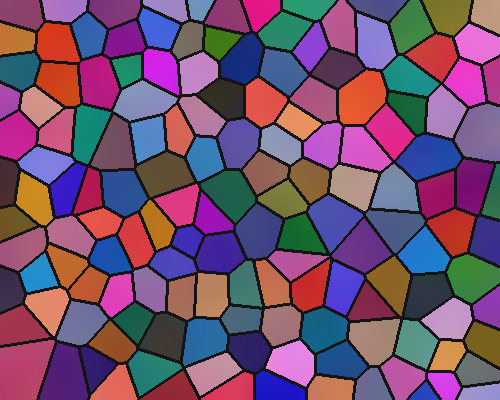
\includegraphics[width=20mm]{assets/drawn/grain-map-wide}};
    \node[anchor=north west,label text,text width=22mm] at (121,-8.4) {EBSD map\\ 1000\,×\,800 px\\ 0.5\,µm per px};
    \node[anchor=north west,label text,text width=42mm] at (98.5,-26.6)
      {colour: $(\varphi_1,\Phi,\varphi_2)\to$ red, green, blue};
    \begin{scope}[shift={(99.5,-48.5)}]
      \draw[udsgreymid,line width=0.5pt] (0,13) -- (0,0) -- (18,0);
      \draw[udsdark,line width=0.9pt] (0,0) -- (1.6,8.2) .. controls (4,10.2) and (12,11.6) .. (15.4,11.2)
        -- (16,8.8);
      \node[circle,fill=udsred,inner sep=0pt,minimum size=1.5mm] at (1.6,8.2) {};
      \node[circle,fill=udsred,inner sep=0pt,minimum size=1.5mm] at (16,8.8) {};
    \end{scope}
    \node[anchor=north west,label text,text width=22mm] at (121,-36.6) {tensile test:\\ yield strength,\\ elongation};
  \end{tikzpicture}
  \note{\textbf{11:30--12:40}\par
    The 25 alloys come from an orthogonal design: five hot-rolling reductions, five annealing
      temperatures and five annealing times, combined so that every pair of levels occurs once.\par
    Each cell is one alloy; the number is its annealing time and the shade its yield strength.\par
    More rolling and lower annealing temperatures give the stronger alloys.\par
    Each alloy has one EBSD map of 1000 by 800 pixels at 0.5 µm per pixel, a field of 500 by 400 µm,
      with the three Euler angles of each pixel stored as red, green and blue.\par
    Each alloy also has one yield strength and one elongation; how many tensile tests stand behind them
      is not stated.\par
    So the dataset is 25 maps and 25 pairs of property values.}
\end{frame}

% ----------------------------------------------------------------- split
\begin{frame}[source={Liao et al.\ (2026), Nat.\ Commun.\ 17, 11232, Results and Methods}]{Alloy split before cropping}
  \begin{tikzpicture}[x=1mm,y=1mm]
    \useasboundingbox (0,0) rectangle (144,-54);
    % stages, left to right
    \foreach \x/\t in {32/{EBSD maps},64/{patches, 100\,×\,100\,px},97/{+ flips, rotations},
        128/{+ degraded copies}}
      \node[anchor=north,label text,align=center] at (\x,0) {\t};
    \node[anchor=north,inner sep=0pt] (m1) at (32,-5.2) {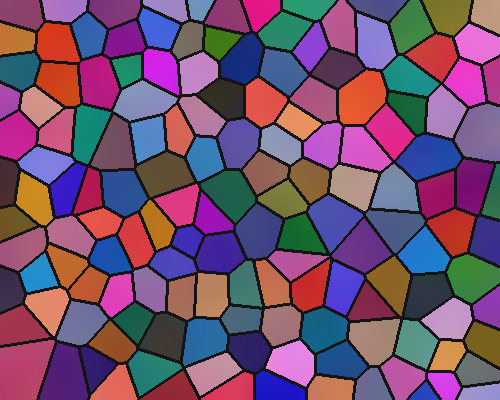
\includegraphics[width=16mm]{assets/drawn/grain-map-wide}};
    \node[anchor=north,inner sep=0pt] (m2) at (64,-5.2) {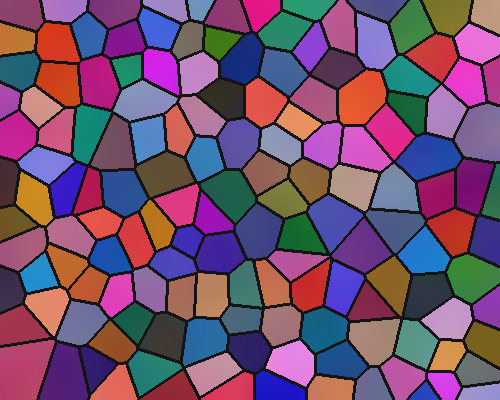
\includegraphics[width=16mm]{assets/drawn/grain-map-wide}};
    \draw[white,line width=0.35pt] \foreach \i in {1,...,9} {([xshift=\i*1.6mm]m2.north west) -- ([xshift=\i*1.6mm]m2.south west)}
      \foreach \j in {1,...,7} {([yshift=-\j*1.6mm]m2.north west) -- ([yshift=-\j*1.6mm]m2.north east)};
    \draw[udsred,line width=0.7pt] (m2.north west) rectangle ([xshift=1.6mm,yshift=-1.6mm]m2.north west);
    \node[inner sep=0pt] at (91.5,-9.7) {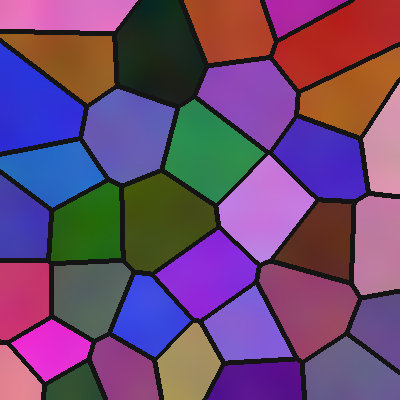
\includegraphics[width=9mm]{assets/drawn/grain-map}};
    \node[inner sep=0pt,rotate=90] at (102.5,-9.7) {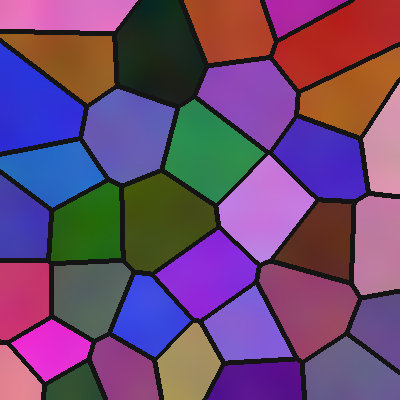
\includegraphics[width=9mm]{assets/drawn/grain-map}};
    \node[inner sep=0pt] at (122.5,-9.7) {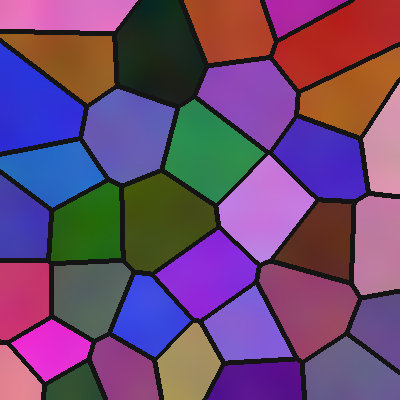
\includegraphics[width=9mm]{assets/drawn/grain-map}};
    \node[inner sep=0pt] at (133.5,-9.7) {
\includegraphics[width=9mm]{assets/drawn/grain-map-blurred}};
    % the two lanes
    \fill[bluetint] (0,-24) rectangle (144,-33.6);
    \fill[redtint] (0,-35.6) rectangle (144,-45.2);
    \node[anchor=west,label text,font=\footnotesize\bfseries,text=udsblue] at (1.6,-28.8) {training};
    \node[anchor=west,label text,font=\footnotesize\bfseries,text=udsred] at (1.6,-40.4) {test};
    \foreach \x/\ta/\tb in {32/{20 alloys}/{5 alloys},64/{1,600}/{400},97/{9,600}/{2,400},128/{57,600}/{14,400}} {
      \node[font=\small\bfseries,text=udsdark,inner sep=0pt] at (\x,-28.8) {\ta};
      \node[font=\small\bfseries,text=udsdark,inner sep=0pt] at (\x,-40.4) {\tb};}
    \foreach \x/\m in {48/\times 80,80.5/\times 6,112.5/\times 6} {
      \draw[flow,draw=udsgreymid] (\x-5,-28.8) -- (\x+5,-28.8);
      \draw[flow,draw=udsgreymid] (\x-5,-40.4) -- (\x+5,-40.4);
      \node[small label,anchor=south] at (\x,-23.4) {$\m$};}
    \goodstrip{-48.4}{test patches come from five alloys the model never sees in training}
  \end{tikzpicture}
  \note{\textbf{12:40--13:30}\par
    The split comes first: the 25 maps are divided at random into 20 training and 5 test alloys.\par
    Only then is each map cut into 80 patches of 100 by 100 pixels, 50 by 50 µm.\par
    Flips and rotations make six versions of each patch.\par
    Each version also gets five degraded copies (blur, distortion, black blocks, erosion and dilation),
      which the model learns to restore.\par
    That gives 72,000 images: 57,600 for training and 14,400 for testing.\par
    Because the split is by alloy, no test patch shares a map with a training patch: the same rule as
      splitting by specimen in segmentation.\par
    The images multiply; the alloys stay 25.}
\end{frame}

% ------------------------------------------------------------- generator
\begin{frame}[source={Liao et al.\ (2026), Nat.\ Commun.\ 17, 11232, Fig.\ 1a (CC BY-NC-ND 4.0) · Pandey et al.\ (2022), Trans.\ Mach.\ Learn.\ Res.}]
  {A VAE, refined by diffusion}
  \begin{tikzpicture}[x=1mm,y=1mm]
    \useasboundingbox (0,0) rectangle (144,-54);
    % Fig. 1a as published: its schematic, without the loss equation below it (pixel rows 0 to 258)
    \figpart{0}{0}{1}{0}{0}{2000}{258}{144}
    % the size of each part, under it; x from the part's pixel columns in the figure
    \tikzset{size/.style={anchor=north,small label,text=udsdark,align=center}}
    \node[size] at ({\fpx{113}},-19.8) {$100\times100$ px};
    \node[size,text=udsred] at ({\fpx{521}},-19.8) {128 numbers};
    \node[size] at ({\fpx{918}},-19.8) {$100\times100$ px};
    \node[size] at ({\fpx{1455}},-19.8) {one U-Net for every step};
    \node[size,anchor=north east] at (144,-19.8) {$100\times100$ px};
    % the two models, each under a bracket
    \draw[udsblue,line width=0.6pt] ({\fpx{40}},-23.6) -- ++(0,-1.4) -| ({\fpx{990}},-23.6);
    \node[anchor=north,label text,align=center,text width=68mm] at ({\fpx{515}},-26.4)
      {\textbf{variational autoencoder (VAE)}\\ three convolutional layers in, three transposed out\\
       loss $L_{\mathrm{pix}}+L_{\mathrm{edge}}+L_{\mathrm{SSIM}}+L_{\mathrm{KL}}$};
    \draw[udsblue,line width=0.6pt] ({\fpx{1148}},-23.6) -- ++(0,-1.4) -| ({\fpx{1997}},-23.6);
    \node[anchor=north,label text,align=center,text width=60mm] at ({\fpx{1572}},-26.4)
      {\textbf{conditional diffusion model (DDPM)}\\ a U-Net predicts the noise, guided by $x_V$\\
       loss: the same three terms on the noise};
    % how the generator is trained, and how it generates
    \foreach \i/\c/\icon/\h/\b in {
        0/udsblue/\faImages/training data/{57,600 images of the 20 training alloys: patches to reproduce,
          and degraded copies to restore},
        1/udsred/\faStar/generation/{a code from the search goes through the decoder, then the diffusion
          model: a new patch}} {
      \fill[\c!8] ({\i*74},-39) rectangle ++(70,-14.6);
      \fill[\c] ({\i*74},-39) rectangle ++(1.2,-14.6);
      \node[anchor=north west,inner sep=0pt,font=\scriptsize\bfseries,text=\c] at ({\i*74+3.4},-40.8)
        {\icon\enspace\h};
      \node[anchor=north west,inner sep=0pt,font=\scriptsize,text=udsdark,text width=64.6mm,align=left,
        execute at begin node={\hyphenpenalty=10000\raggedright}] at ({\i*74+3.4},-44.8) {\b};}
  \end{tikzpicture}
  \note{\textbf{13:30--14:20}\par
    This is the paper's own diagram of its generator, Fig.~1a.\par
    The VAE compresses each patch of 100 by 100 pixels into a code z of 128 numbers and decodes it into
      $x_V$, which is smooth.\par
    A conditional diffusion model then refines $x_V$: its U-Net predicts the noise step by step and sees
      $x_V$ at every step, the pairing of DiffuseVAE; the red arrow marks that condition.\par
    Both models are trained with the pixel, edge and SSIM terms of the next slide: the VAE on its output,
      the diffusion model on the noise it predicts.\par
    Training uses the 57,600 images of the 20 training alloys, with Adam over 100 epochs.\par
    The code z is what the search moves around later.}
\end{frame}

% ------------------------------------------------------------------ loss
\begin{frame}[source={Liao et al.\ (2026), Nat.\ Commun.\ 17, 11232, Eqs.\ 1--9 · Sobel and Feldman (1968), Stanford AI Project · Wang et al.\ (2004), IEEE Trans.\ Image Process.\ 13, 600}]{Optimization Loss}
  \begin{tikzpicture}[x=1mm,y=1mm]
    \useasboundingbox (0,0) rectangle (144,-54);
    % the equation, each term above its column
    \foreach \x/\t in {5/{L\;=},22/{L_{\mathrm{pix}}},47/{+},72/{\color{udsblue}L_{\mathrm{edge}}},97/{+},
        122/{\color{udsblue}L_{\mathrm{SSIM}}}}
      \node[font=\LARGE,text=udsdark,inner sep=0pt] at (\x,-3.2) {$\t$};
    \foreach \x/\c/\h in {0/udsgreymid/{pixel values},50/udsblue/{edges},100/udsblue/{structure}} {
      \fill[\c!8] (\x,-16.6) rectangle ++(44,-35.4);
      \cardhead{\x}{-11.2}{44}{\c}{\h}}
    % pixel values
    \node[anchor=north,font=\small,text=udsdark,inner sep=0pt] at (22,-19.6)
      {$\displaystyle\frac{1}{n}\sum_{i=1}^{n}|x_i-\hat{x}_i|$};
    \node[anchor=north west,card text,text width=40mm] at (2,-31)
      {Mean Absolute\\ Difference (MAE)\\[0.8mm] every pixel weighs the same; boundaries are few pixels};
    % edges
    \node[anchor=north,font=\small,text=udsdark,inner sep=0pt] at (72,-19.6)
      {$\mathrm{mean}\,|S\ast x-S\ast\hat{x}|$};
    \node[anchor=north west,inner sep=0pt] (e1) at (54,-25.4) {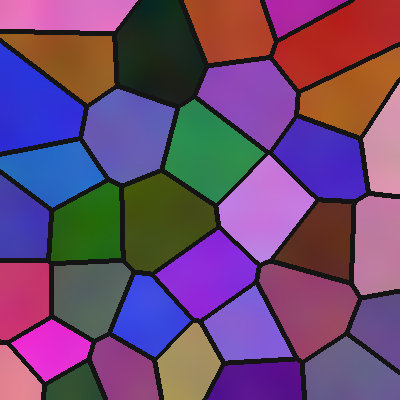
\includegraphics[width=12mm]{assets/drawn/grain-map}};
    \node[anchor=north west,inner sep=0pt] (e2) at (78,-25.4) {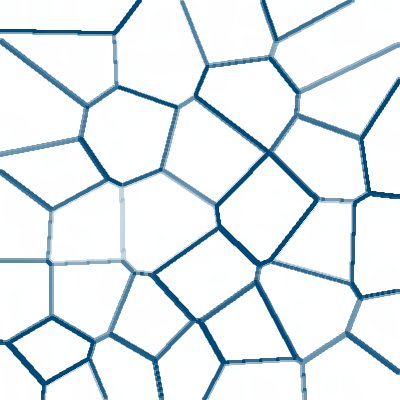
\includegraphics[width=12mm]{assets/drawn/grain-map-edges}};
    \draw[icon frame,udsgreylight] (e2.south west) rectangle (e2.north east);
    \draw[flow,draw=udsblue] (e1.east) -- node[above=0.6mm,small label,text=udsblue] {$S\ast$} (e2.west);
    \node[anchor=north west,card text,text width=40mm] at (52,-40)
      {Sobel filter $S$, across and down: large at grain boundaries};
    % structure
    \node[anchor=north,font=\small,text=udsdark,inner sep=0pt] at (122,-19.6)
      {$1-\mathrm{SSIM}(x,\hat{x})$};
    \node[anchor=north west,inner sep=0pt] (s1) at (104,-25.4) {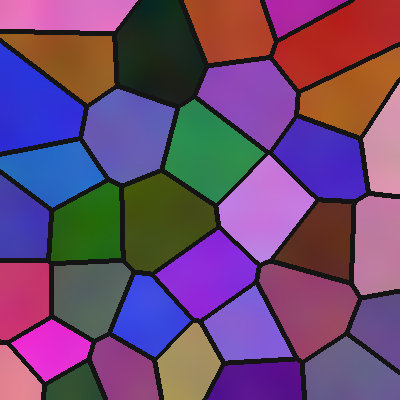
\includegraphics[width=12mm]{assets/drawn/grain-map}};
    \node[anchor=north west,inner sep=0pt] (s2) at (128,-25.4) {
\includegraphics[width=12mm]{assets/drawn/grain-map-blurred}};
    \node[small label,text=udsblue] at (122,-31.4) {$x$ vs $\hat{x}$};
    \node[anchor=north west,card text,text width=40mm] at (102,-40)
      {means, contrasts and correlation: orientation inside grains};
  \end{tikzpicture}
  \note{\textbf{14:20--15:30}\par
    The loss is the sum of three terms, added without weights.\par
    The pixel term is the mean absolute difference between original and reconstruction; boundaries
      cover few pixels, so it hardly sees them.\par
    The edge term applies the Sobel filter, a three-by-three derivative filter from Sobel and Feldman,
      1968, across and down both images and compares the responses: it is large where colours change,
      at grain boundaries.\par
    The structure term is one minus the structural similarity index (SSIM) of Wang and colleagues, 2004,
      which compares the means, contrasts and correlation of the two images; the authors use it for the
      orientation inside and between grains.\par
    The VAE adds its Kullback--Leibler term; the diffusion model applies the same three terms to the
      noise it predicts.\par
    All three compare colours, that is, Euler angles read as intensities.}
\end{frame}

% ------------------------------------------------------------------ SSIM
\begin{frame}[source={Liao et al.\ (2026), Nat.\ Commun.\ 17, 11232, Eqs.\ 4--9 · Wang et al.\ (2004), IEEE Trans.\ Image Process.\ 13, 600}]{Structural Similarity (SSIM)}
  \begin{tikzpicture}[x=1mm,y=1mm]
    \useasboundingbox (0,0) rectangle (144,-54);
    \tikzset{pair image/.style={anchor=north west,inner sep=0pt},
      component value/.style={anchor=north,inner sep=0pt,font=\scriptsize,text=udsdark},
      component formula/.style={anchor=north,inner sep=0pt,font=\footnotesize,text=udsdark},
      component meaning/.style={anchor=north,inner sep=0pt,font=\scriptsize,text=udsdark}}
    % three components; each compares the patch with a copy that changes only what it measures
    \foreach \i/\h in {0/{luminance $L$},1/{contrast $C$},2/{structure $S$}} {
      \fill[bluetint] ({\i*49},-5.4) rectangle ++(46,-29.4);
      \cardhead{\i*49}{0}{46}{udsblue}{\h}
      \node[pair image] at ({\i*49+7.4},-7.4) {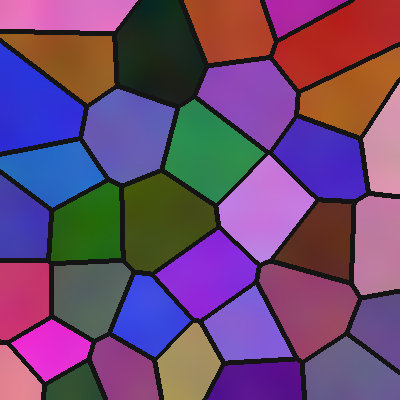
\includegraphics[width=11mm]{assets/drawn/grain-map}};
      \node[small label,text=udsdark] at ({\i*49+23},-12.9) {vs};}
    \node[pair image] at (28.6,-7.4) {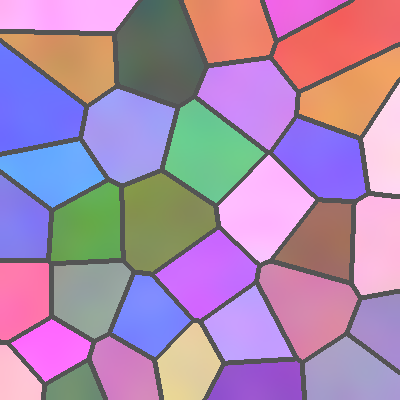
\includegraphics[width=11mm]{assets/drawn/ssim-bright}};
    \node[pair image] at (77.6,-7.4) {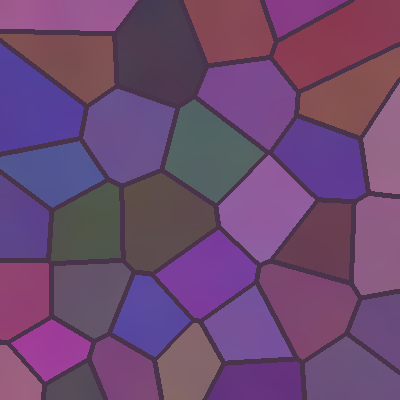
\includegraphics[width=11mm]{assets/drawn/ssim-flat}};
    \node[pair image] at (126.6,-7.4) {
\includegraphics[width=11mm]{assets/drawn/ssim-shuffled}};
    \node[component value] at (23,-19.6)
      {\textcolor{udsred}{$L=\ssimBrightL$}\enspace $C=\ssimBrightC$\enspace $S=\ssimBrightS$};
    \node[component value] at (72,-19.6)
      {$L=\ssimFlatL$\enspace \textcolor{udsred}{$C=\ssimFlatC$}\enspace $S=\ssimFlatS$};
    \node[component value] at (121,-19.6)
      {$L=\ssimShuffledL$\enspace $C=\ssimShuffledC$\enspace \textcolor{udsred}{$S=\ssimShuffledS$}};
    \node[component formula] at (23,-23.2) {$\dfrac{2\mu_x\mu_{\hat x}+C_1}{\mu_x^2+\mu_{\hat x}^2+C_1}$};
    \node[component formula] at (72,-23.2) {$\dfrac{2\sigma_x\sigma_{\hat x}+C_2}{\sigma_x^2+\sigma_{\hat x}^2+C_2}$};
    \node[component formula] at (121,-23.2) {$\dfrac{\sigma_{x\hat x}+C_3}{\sigma_x\sigma_{\hat x}+C_3}$};
    \node[component meaning] at (23,-31) {brightness: the means $\mu$};
    \node[component meaning] at (72,-31) {contrast: the spreads $\sigma$};
    \node[component meaning] at (121,-31) {pattern: the covariance $\sigma_{x\hat x}$};
    % multiplied as the paper does, and turned into a loss
    \fill[bluetint] (0,-37.6) rectangle (144,-53.6);
    \node[anchor=west,inner sep=0pt,font=\footnotesize,text=udsdark] at (2.4,-42.6)
      {$\mathrm{SSIM}=L^{\alpha}\,C^{\beta}\,S^{\gamma}$};
    \node[anchor=west,small label,text=udsdark,text width=44mm] at (2.4,-48.8)
      {paper: $\alpha=\beta=\gamma=1$, $C_3=C_2/2$};
    \node[anchor=west,inner sep=0pt,font=\footnotesize,text=udsdark] (eq8) at (46.6,-45.6)
      {$=\dfrac{(2\mu_x\mu_{\hat x}+C_1)(2\sigma_{x\hat x}+C_2)}{(\mu_x^2+\mu_{\hat x}^2+C_1)(\sigma_x^2+\sigma_{\hat x}^2+C_2)}$};
    \draw[flow,draw=udsblue] ([xshift=1.6mm]eq8.east) -- ++(5.4,0);
    \node[anchor=west,inner sep=0pt,font=\footnotesize,text=udsdark] (loss) at ([xshift=8.6mm]eq8.east)
      {$L_{\mathrm{SSIM}}=1-\mathrm{SSIM}$};
    \node[anchor=north west,small label,text=udsdark] at ([yshift=-1.4mm]loss.south west) {zero for identical patches};
  \end{tikzpicture}
  \note{\textbf{15:30--16:40}\par
    SSIM compares two patches in three ways, each through one statistic of the pixel values.\par
    Luminance compares the means: a brighter copy of the patch scores $L=\ssimBrightL$, while $C$ and $S$
      stay near 1.\par
    Contrast compares the standard deviations: a flattened copy scores $C=\ssimFlatC$.\par
    Structure compares the patterns through the covariance: shuffling the patch's tiles keeps its mean
      and spread but drops $S$ to \ssimShuffledS.\par
    The product, with all exponents 1 and $C_3=C_2/2$ as in the paper, gives its Eq.~8; the loss is one
      minus SSIM.\par
    The brighter copy differs by \ssimBrightM{} per pixel on average and keeps SSIM \ssimBrightQ; the blurred
      patch of slide 4 differs by only \ssimBlurredM{} but drops to \ssimBlurredQ: SSIM sees lost structure
      that a pixel loss barely notices.}
\end{frame}

% --------------------------------------------------- failure case, fixed
\begin{frame}[source={Liao et al.\ (2026), Nat.\ Commun.\ 17, 11232, Fig.\ 2c (CC BY-NC-ND 4.0)}]
  {The same patches, with the new loss}
  \begin{tikzpicture}[x=1mm,y=1mm]
    \useasboundingbox (0,0) rectangle (144,-54);
    \figpart{36}{0}{2}{340}{770}{1897}{1537}{104}
    \node[anchor=east,label text,align=right] at (33,{\fpy{884}}) {real patches};
    \node[anchor=east,label text,align=right,text=udsred] at (33,{\fpy{1155}}) {pixel loss only};
    \node[anchor=east,label text,align=right,text=testgreen] at (33,{\fpy{1423}}) {with edge and\\SSIM terms};
  \end{tikzpicture}
  \note{\textbf{16:40--17:20}\par
    The same six test patches, with a third row: the model trained with all three terms.\par
    The boundaries are sharp again, and each grain has nearly one colour.\par
    The pixel loss itself also falls, from about 0.20 to about 0.10 according to the text; the plotted
      curve settles nearer 0.07.\par
    Two more reconstruction terms also weaken the Kullback--Leibler term relative to the rest, which by
      itself can lower a VAE's reconstruction error; the paper does not separate the two effects.\par
    The comparison with a standard VAE, a Wasserstein GAN and a standard DDPM is only in the
      Supplementary Information.}
\end{frame}

% ------------------------------------------------------------ descriptor
\begin{frame}[source={Liao et al.\ (2026), Nat.\ Commun.\ 17, 11232, after Fig.\ 4a and Methods · Pearson (1901), Philos.\ Mag.\ 2, 559}]{Six numbers per alloy}
  \begin{tikzpicture}[x=1mm,y=1mm]
    \useasboundingbox (0,0) rectangle (144,-54);
    \tikzset{dims/.style={anchor=north,small label,text=udsdark,align=center},
      op/.style={small label,text=udsgrey,align=center},
      back/.style={anchor=north,small label,text=udsred,align=center}}
    % one alloy's map, cut into 10 x 8 patches of 100 x 100 pixels
    \node[anchor=north west,inner sep=0pt] at (0,0) {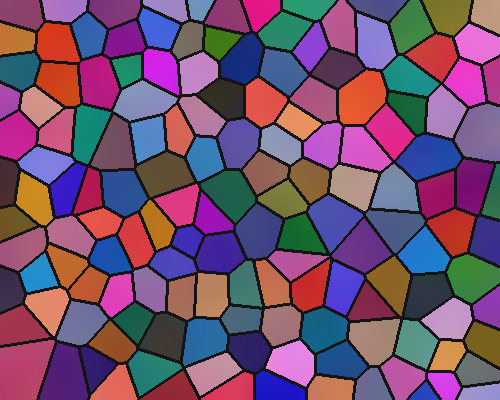
\includegraphics[width=25mm]{assets/drawn/grain-map-wide}};
    \draw[white,line width=0.35pt] \foreach \i in {1,...,9} {(\i*2.5,0) -- (\i*2.5,-20)}
      \foreach \j in {1,...,7} {(0,-\j*2.5) -- (25,-\j*2.5)};
    \node[dims] at (12.5,-20.8) {one alloy, $1000\times800$ px:\\ 80 patches};
    % the encoder gives one code of 128 numbers per patch
    \draw[flow] (25.6,-10) -- (28.2,-10);
    \filldraw[fill=bluetint,draw=udsblue,line width=0.5pt] (28.8,-3.4) -- (36.4,-6.8) -- (36.4,-13.2) -- (28.8,-16.6) -- cycle;
    \node[label text,rotate=90,font=\scriptsize] at (32.4,-10) {encoder};
    \draw[flow] (37,-10) -- (39.6,-10);
    \codematrix{40.2}{-1}{16}{18}{1}
    \node[dims] at (48.2,-20.8) {80 codes\\ $\times$ 128 numbers};
    % mean and spread over the 80 patches
    \draw[flow] (56.8,-7.2) -- node[above=0.4mm,op,sloped] {mean} (65.4,-5.4);
    \draw[flow] (56.8,-12.8) -- node[below=0.4mm,op,sloped] {spread} (65.4,-14.6);
    \pgfmathsetseed{80}
    \foreach \c in {0,...,15} {
      \pgfmathtruncatemacro\shadeA{20+50*rnd}
      \pgfmathtruncatemacro\shadeB{10+45*rnd}
      \filldraw[fill=udsblue!\shadeA,draw=udsblue,line width=0.3pt] ({66+1.25*\c},-4.2) rectangle ++(1.25,-2.4);
      \filldraw[fill=udsdark!\shadeB,draw=udsdark,line width=0.3pt] ({66+1.25*\c},-13.4) rectangle ++(1.25,-2.4);}
    \node[anchor=south,small label,text=udsdark] at (76,-3.6) {$\mu$: 128 numbers};
    \node[dims] at (76,-16.4) {$\sigma$: 128 numbers};
    % PCA, fitted on the 25 alloys: the first three components of each
    \draw[flow] (86.6,-5.4) -- node[above=0.4mm,op] {PCA} (92.4,-5.4);
    \draw[flow] (86.6,-14.6) -- node[below=0.4mm,op] {PCA} (92.4,-14.6);
    \foreach \j in {0,1,2} {
      \filldraw[fill=bluetint,draw=udsblue,line width=0.5pt] ({93+2.4*\j},-4.2) rectangle ++(2.4,-2.4);
      \filldraw[fill=darktint,draw=udsdark,line width=0.5pt] ({93+2.4*\j},-13.4) rectangle ++(2.4,-2.4);}
    \node[op,anchor=north] at (96.6,-19.6) {first 3 of\\ 24 components};
    % the descriptor
    \draw[flow] (100.8,-5.4) to[out=0,in=180] (107.4,-9.4);
    \draw[flow] (100.8,-14.6) to[out=0,in=180] (107.4,-10.6);
    \descstrip{108}{-8.8}{2.4}{2.4}
    \node[anchor=south,small label,text=udsdark] at (115.2,-8.2) {descriptor};
    \node[anchor=west,small label,text=udsdark] at (123.2,-10) {6 numbers};
    % the table it fills: one row per alloy, beside the measured properties
    \draw[flow] (115.2,-11.6) -- (115.2,-31.8);
    \descstrip{108}{-32.4}{2.4}{3}
    \foreach \x/\l in {122.4/YS,129.4/El}
      \node[draw=udsgreymid,fill=darktint,line width=0.3pt,minimum width=7mm,minimum height=3mm,inner sep=0pt,
        anchor=north west,font=\scriptsize,text=udsdark] at (\x,-32.4) {\l};
    \foreach \r in {1,...,3} \foreach \x/\w in {108/14.4,122.4/7,129.4/7}
      \draw[udsgreylight,line width=0.3pt,fill=white] (\x,{-32.4-3*\r}) rectangle ++(\w,-3);
    \node[small label,text=udsdark] at (122.4,-45.4) {$\vdots$};
    \node[dims,text width=36mm] at (122.4,-48.9) {25 alloys: six numbers, yield strength, elongation};
    % the way back, which the search uses: below the labels, up to the map's label at the end
    \draw[udsred,line width=0.6pt,dash pattern=on 1.6pt off 1.2pt,-{Stealth[length=1.6mm,width=1.2mm]}]
      (109.2,-11.6) -- (109.2,-31) -- (12.5,-31) -- (12.5,-27.6);
    \foreach \x/\l in {96.6/inverse PCA,76/{$\mu$, $\sigma$},48.2/draw 80 codes,32.6/decode}
      \node[back] at (\x,-31.8) {\l};
    \node[anchor=north west,small label,text=udsred,text width=92mm] at (0,-36.4)
      {the way back, for the search: six numbers give a mean and a spread, 80 codes are drawn from them and
       decoded into new patches};
  \end{tikzpicture}
  \note{\textbf{17:20--18:10}\par
    To link microstructures with properties, each alloy needs one descriptor.\par
    The 80 patches of its map are encoded, which gives 80 codes of 128 numbers.\par
    Their mean and standard deviation over the patches describe the alloy: what its patches look like
      on average, and how much they vary.\par
    Principal component analysis (PCA, Pearson 1901), fitted on the 25 alloys, keeps the first three of
      24 components of each, so every alloy becomes six numbers beside its measured properties.\par
    PCA can be inverted, the red path: six numbers map back to a mean and a spread, from which new codes
      are drawn and decoded.\par
    The number of components was chosen by the fidelity of the generated patches (Supplementary
      Information).}
\end{frame}

% ---------------------------------------------------------------- search
\begin{frame}[source={Liao et al.\ (2026), Nat.\ Commun.\ 17, 11232, after Fig.\ 4a · Deb et al.\ (2002), IEEE Trans.\ Evol.\ Comput.\ 6, 182}]{A genetic search in six numbers}
  \begin{tikzpicture}[x=1mm,y=1mm]
    \useasboundingbox (0,0) rectangle (144,-54);
    \tikzset{glyph label/.style={anchor=north,small label,text=udsdark,align=center},
      op/.style={anchor=south,small label,text=udsgrey,align=center,yshift=1mm}}
    % the loop: four steps on cards, run for 500 generations
    \foreach \i/\h in {0/population,1/predict,2/keep the best,3/{cross over, mutate}} {
      \pgfmathsetmacro\cx{\i*38}
      \fill[bluetint] (\cx,-5.4) rectangle ++(30,-13.4);
      \cardhead{\cx}{0}{30}{udsblue}{\h}}
    \foreach \i in {0,1,2} \draw[flow,draw=udsblue] ({\i*38+30.4},-12.1) -- ({\i*38+37.6},-12.1);
    % population: 10 descriptors of six numbers
    \foreach \k in {0,...,4} {\descstrip{4}{-7-1.7*\k}{1.5}{1.2}\descstrip{17}{-7-1.7*\k}{1.5}{1.2}}
    \node[glyph label] at (15,-15.6) {10 descriptors};
    % predict: one tree model per property
    \minitree{45.5}{-7.2}
    \minitree{60.5}{-7.2}
    \node[glyph label] at (45.5,-14.2) {strength};
    \node[glyph label] at (60.5,-14.2) {elongation};
    % keep the best: fronts and crowding, as on slide 10
    \begin{scope}[shift={(80.5,-17.4)}]
      \draw[udsgreymid,line width=0.4pt] (0,10.4) -- (0,0) -- (22,0);
      \begin{scope}[x=22mm,y=10mm]
        \drawfronttwo[udsgreymid,line width=0.5pt,dash pattern=on 1.2pt off 0.9pt]
        \drawfrontone[udsblue,line width=0.7pt]
        \foreach \x/\y/\r in \paretopoints {
          \ifcase\r\or\def\rc{udsblue}\or\def\rc{udsgreymid}\else\def\rc{udsgreylight}\fi
          \node[circle,fill=\rc,inner sep=0pt,minimum size=1.2mm] at (\x,\y) {};}
      \end{scope}
    \end{scope}
    % cross over and mutate: a child from two parents, one number changed
    \foreach \j in {0,...,5} {
      \filldraw[fill=udsblue!20,draw=udsblue,line width=0.3pt] ({116.6+1.8*\j},-7.4) rectangle ++(1.8,-1.8);
      \filldraw[fill=udsblue!65,draw=udsblue,line width=0.3pt] ({116.6+1.8*\j},-10.4) rectangle ++(1.8,-1.8);
      \ifnum\j<3\def\cf{udsblue!20}\else\def\cf{udsblue!65}\fi
      \ifnum\j=4\def\cf{udsred!70}\fi
      \filldraw[fill=\cf,draw=udsblue,line width=0.3pt] ({131.4+1.8*\j},-8.9) rectangle ++(1.8,-1.8);}
    \draw[flow,draw=udsblue,line width=0.5pt] (128.4,-9.8) -- (130.8,-9.8);
    \node[glyph label] at (122,-13.4) {parents};
    \node[glyph label] at (136.8,-13.4) {child, one\\ number mutated};
    % 500 generations: the way round
    \draw[flow,draw=udsblue] (129,-18.8) -- (129,-21.8) -- (15,-21.8) -- (15,-19.2);
    \node[fill=white,inner sep=1mm,font=\footnotesize\bfseries,text=udsblue] at (72,-21.8) {500 generations};
    % the way back to microstructures, for the 5 best
    \draw[flow] (5,-18.8) -- (5,-30.8);
    \node[anchor=west,small label,text=udsdark] at (6.4,-25) {the 5 best};
    \foreach \k in {0,...,4} \descstrip{0}{-31.4-1.8*\k}{1.8}{1.3}
    \node[glyph label] at (5.4,-41.6) {5 descriptors};
    \draw[flow] (12.2,-36) -- node[op] {inverse\\ PCA} (26.4,-36);
    \pgfmathsetseed{80}
    \foreach \c in {0,...,15} {
      \pgfmathtruncatemacro\shadeA{20+50*rnd}
      \pgfmathtruncatemacro\shadeB{10+45*rnd}
      \filldraw[fill=udsblue!\shadeA,draw=udsblue,line width=0.3pt] ({27.2+1.25*\c},-32.6) rectangle ++(1.25,-2.4);
      \filldraw[fill=udsdark!\shadeB,draw=udsdark,line width=0.3pt] ({27.2+1.25*\c},-37) rectangle ++(1.25,-2.4);}
    \node[glyph label] at (37.2,-40.2) {$\mu$, $\sigma$: 128 each};
    \draw[flow] (48,-36) -- node[op] {draw\\ 80 codes} (62.2,-36);
    \codematrix{63}{-30.6}{12}{11}{1}
    \node[glyph label] at (69,-42.4) {80 codes};
    \draw[flow] (75.8,-36) -- node[op] {decode,\\ refine} (90,-36);
    \node[anchor=north west,inner sep=0pt] at (90.8,-29.6) {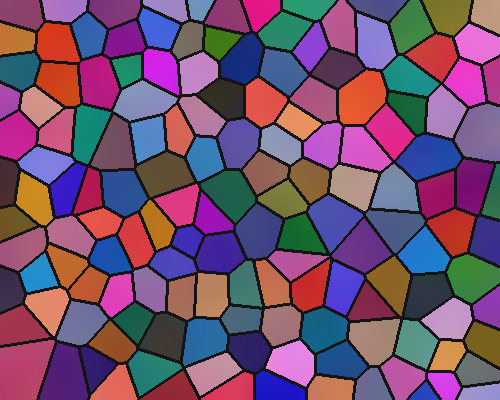
\includegraphics[width=25mm]{assets/drawn/grain-map-wide}};
    \draw[white,line width=0.35pt] \foreach \i in {1,...,9} {(90.8+\i*2.5,-29.6) -- (90.8+\i*2.5,-49.6)}
      \foreach \j in {1,...,7} {(90.8,-29.6-\j*2.5) -- (115.8,-29.6-\j*2.5)};
    \node[glyph label] at (103.3,-50.2) {80 new patches};
    \node[text=udsred,font=\small] at (120.2,-34.4) {\faStar};
    \node[anchor=north west,label text,text width=21mm,text=udsred] at (122.6,-32.4)
      {a proposed microstructure for each descriptor};
  \end{tikzpicture}
  \note{\textbf{18:10--19:00}\par
    The loop of section 2, run on the six numbers.\par
    Two gradient-boosted tree models, one per property, fitted on the 20 training alloys, predict yield
      strength and elongation from a descriptor; they are the objectives.\par
    NSGA-II evolves a population of 10 descriptors over 500 generations; the paper's average hypervolume
      improvement, the area the candidates span above the weakest measured alloy, levels off after about
      150 generations.\par
    The five best final descriptors go back through the inverse PCA to a mean and a spread; 80 codes are
      drawn from them and decoded into patches, the proposed microstructures.}
\end{frame}

\section[Results]{The results}
\sectionframe{04}{The results}{What do the authors show?}{\faChartBar}

% ------------------------------------------------------------ fidelity
\begin{frame}[source={Liao et al.\ (2026), Nat.\ Commun.\ 17, 11232, Fig.\ 3i--n (CC BY-NC-ND 4.0)}]
  {Grain statistics after reconstruction}
  \begin{tikzpicture}[x=1mm,y=1mm]
    \useasboundingbox (0,0) rectangle (144,-54);
    \figpart{0}{0}{3}{0}{700}{2000}{1883}{91}
    % the two rows of panels, by the figure's own panel letters
    \node[anchor=north west,label text,text width=46mm] at (98,-0.6) {original against reconstruction};
    \node[anchor=west,label text,text width=46mm] at (98,-8.4) {\textbf{i--k}\enspace grain area and ellipse axes};
    \node[anchor=west,label text,text width=46mm] at (98,-13.8) {\textbf{l--n}\enspace the three Euler angles};
    \node[circle,fill=udsgreylight,inner sep=0pt,minimum size=2mm] at (99.4,-20.6) {};
    \node[anchor=west,label text,text width=41mm] at (102,-20.6) {2,000 single patches: wide scatter};
    \node[circle,fill=udsblue!75,inner sep=0pt,minimum size=2mm] at (99.4,-27.4) {};
    \node[anchor=west,label text,text width=41mm] at (102,-27.4) {20 training alloys, each the mean of 80 patches};
    \node[rectangle,fill=udsred!80,inner sep=0pt,minimum size=2mm] at (99.4,-34.2) {};
    \node[anchor=west,label text,text width=41mm] at (102,-34.2) {5 test alloys};
    \draw[udsred,line width=0.6pt,dash pattern=on 1.4pt off 1pt] (98,-39.6) -- (100.8,-39.6);
    \node[anchor=west,label text] at (102,-39.6) {reconstruction = original};
  \end{tikzpicture}
  \note{\textbf{19:10--20:00}\par
    Six features are measured in each original patch and its reconstruction: grain area, the major
      and minor axes of the equivalent ellipse (panels i to k), and the three Euler angles (l to n).\par
    The grey points are the 2,000 single patches; their means scatter widely, more so for large grains,
      of which one patch holds only a few.\par
    Averaged over the 80 patches of each alloy, the 20 training alloys in blue and the 5 test alloys in
      red lie on the line of equality.\par
    So the model reproduces the grain statistics of alloys it never saw.\par
    What is compared: reconstructions with their own inputs, the first task of slide 7.\par
    Misorientation statistics and the baseline models are in the Supplementary Information only.}
\end{frame}

% ---------------------------------------------------------- surrogates
\begin{frame}[source={Liao et al.\ (2026), Nat.\ Commun.\ 17, 11232, Fig.\ 4b, c (CC BY-NC-ND 4.0) · Friedman (2001), Ann.\ Stat.\ 29, 1189}]
  {Property predictions}
  \begin{tikzpicture}[x=1mm,y=1mm]
    \useasboundingbox (0,0) rectangle (144,-54);
    \figpart{6}{0}{4}{0}{480}{640}{975}{62}
    \figpart{78}{0}{4}{640}{480}{1260}{975}{60.1}
    \node[anchor=north west,label text,text width=144mm] at (6,-50)
      {Gradient-Boosted Trees on the six numbers: fitted on 20 alloys, tested on 5};
  \end{tikzpicture}
  \note{\textbf{20:00--20:40}\par
    These are two gradient-boosted tree models (Friedman, 2001), one per property: sums of many small
      regression trees on an alloy's six numbers; the number of trees and their depth were set by a
      randomized search.\par
    On the five test alloys, R² is 0.96 for yield strength and 0.92 for elongation; on the 20 training
      alloys 0.96 and 0.93.\par
    R² is the share of the variance of the measured values that the predictions explain.\par
    These two models are what the search optimizes.}
\end{frame}

% ---------------------------------------------------------- candidates
\begin{frame}[source={Liao et al.\ (2026), Nat.\ Commun.\ 17, 11232, after Fig.\ 4f; Fig.\ 4e (CC BY-NC-ND 4.0)}]
  {Five candidates beyond the front}
  \begin{tikzpicture}[x=1mm,y=1mm]
    \useasboundingbox (0,0) rectangle (144,-54);
    \begin{scope}[shift={(14,-41)}]
      \planeaxes{340}{1000}{28}{86}{76}{41}{400,500,...,1000}{30,40,...,80}
      \begin{scope}[plane]
        \drawfront[front]
        \drawalloys
        \drawcandidates
        \node[anchor=west,inner sep=0pt] at ([xshift=1.4mm]cand1.east) {\candlabel{1}};
        \node[anchor=west,inner sep=0pt] at ([xshift=1.4mm]cand2.east) {\candlabel{2}};
      \end{scope}
      \node[alloy] at (52,39.4) {};
      \node[anchor=west,small label,text=udsdark] at (54,39.4) {measured};
      \node[candidate] at (52,35.4) {};
      \node[anchor=west,small label,text=udsdark] at (54,35.4) {candidates};
    \end{scope}
    \node[axis label] at (52,-48.4) {yield strength (MPa)};
    \node[axis label,rotate=90] at (3,-20.5) {elongation (\%)};
    % the latent plane of Fig. 4e
    \figpart{95}{0}{4}{1280}{480}{2000}{975}{49}
    \node[anchor=north west,small label,text width=49mm] at (95,-35.6)
      {first principal components of mean and spread: generated (red) beside measured (grey)};
  \end{tikzpicture}
  \note{\textbf{20:40--21:40}\par
    After 500 generations the search returns five candidates, here with their predicted properties.\par
    All five lie above the measured front: at equal strength, they are predicted to stretch more.\par
    Their predicted values stay inside the ranges of the 25 measured alloys; the gain lies in their
      combination.\par
    On the right, the first principal components of the mean and the spread: measured alloys in grey,
      generated microstructures as triangles, darker for a larger hypervolume improvement.\par
    The best candidates lie far from every measured alloy; the authors call them out of distribution,
      the third task of slide 7.\par
    Candidates 1 and 2 are the ones checked by simulation.}
\end{frame}

% --------------------------------------------------------- fine grains
\begin{frame}[source={Liao et al.\ (2026), Nat.\ Commun.\ 17, 11232, Fig.\ 5a--d (CC BY-NC-ND 4.0) · Ma and Zhu (2017), Mater.\ Today 20, 323}]
  {Fine grains in the generated patches}
  \begin{tikzpicture}[x=1mm,y=1mm]
    \useasboundingbox (0,0) rectangle (144,-54);
    \figpart{0}{0}{5}{0}{0}{1300}{965}{72}
    % generated patches and their histogram, by the figure's own panel letters
    \node[anchor=west,label text,text width=60mm] at (80,-2.6) {\textbf{b}\enspace fine-grain regions, marked by arrows};
    \node[anchor=west,label text,text width=60mm] at (80,-8) {\textbf{d}\enspace more grains in the smallest bin};
    % the proposed mechanism, on an illustrative map
    \node[anchor=north west,small label] at (80,-13.6) {proposed mechanism};
    \node[anchor=north west,inner sep=0pt] (bm) at (80,-17.4) {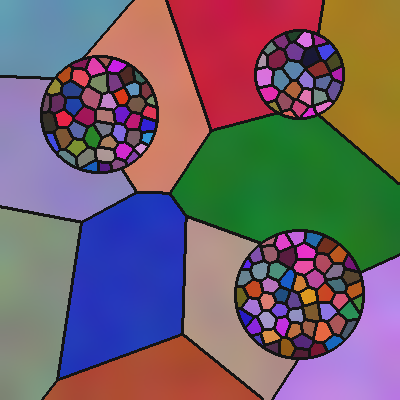
\includegraphics[width=20mm]{assets/drawn/grain-map-bimodal}};
    \node[anchor=west,label text] (fine) at (104,-21.4) {fine grains};
    \draw[udsdark,line width=0.4pt] (fine.west) -- ++(-1.6,0) -- (95,-21.15);
    \node[anchor=west,label text] (coarse) at (104,-28.4) {coarse grains};
    \draw[udsdark,line width=0.4pt] (coarse.west) -- ++(-1.6,0) -- (98,-26.9);
    \node[anchor=north west,card text,text width=63mm] at (80,-39.6)
      {\cardbullet{fine grains block dislocations: strength}
       \cardbullet{coarse grains let them glide: ductility}
       \cardbullet{the mismatch stores dislocations: hardening}};
  \end{tikzpicture}
  \note{\textbf{21:40--22:40}\par
    Left, patches of the initial alloys and patches generated for the candidates; the arrows mark what
      the authors call fine-grain regions (panel b).\par
    Below, the grain areas of all 2,000 original patches and of 400 generated ones, on a logarithmic
      axis: the generated patches have more grains in the smallest bin, at or below 0.4 µm² (panel d),
      which the authors read as a bimodal grain size.\par
    Their explanation: fine grains block dislocations and raise the strength, coarse grains leave room
      for them to glide and keep the ductility, and the mismatch between the two stores geometrically
      necessary dislocations (GNDs), which raise the strain hardening.\par
    The mechanism is established for heterogeneous microstructures; whether these generated patches
      show it remains to be checked.}
\end{frame}

% ------------------------------------------------------------ validation
\begin{frame}[source={Liao et al.\ (2026), Nat.\ Commun.\ 17, 11232, Fig.\ 5e, h (CC BY-NC-ND 4.0)}]
  {Simulation and one experiment}
  \begin{tikzpicture}[x=1mm,y=1mm]
    \useasboundingbox (0,0) rectangle (144,-54);
    \figpart{0}{0}{5}{1430}{49}{1908}{434}{54}
    \node[anchor=north west,label text,text width=54mm] at (0,-46.6)
      {new alloy, route from the literature: 60\,\% rolling at 1000\,°C, 5\,min at 850\,°C};
    \figpart{60}{0}{5}{660}{972}{2000}{1473}{84}
    \node[anchor=north west,label text,text width=84mm] at (60,-33.6)
      {candidate \candlabel{1}: i predicted, ii simulated by crystal plasticity (CPFE), iii measured on
       the new alloy};
  \end{tikzpicture}
  \note{\textbf{22:40--23:40}\par
    Two checks follow.\par
    First, crystal plasticity finite element (CPFE) simulations of two generated patches per candidate,
      with a slip model calibrated on three measured stress--strain curves; the Euler angles come from
      the pixel colours, the dislocation density from a learned mapping.\par
    Second, one experiment: an alloy processed by a route the authors chose from the literature to get
      a bimodal grain size, 60 percent hot rolling at 1000 °C and 5 minutes at 850 °C.\par
    Its EBSD map, left, shows coarse grains among many fine ones.\par
    Right, candidate 1 as predicted, simulated and measured: yield strength about 820, 805 and 825 MPa,
      elongation about 48, 44.5 and 43.5 percent, read from the bars.\par
    The paper concludes that the design is validated.}
\end{frame}

% --------------------------------------------------------------- thank you
% the thanks where the title slide has its title; drawn inside the frame, so that the notes' thumbnail
% shows it too
\begin{frame}[plain,noframenumbering]
\vbox to 0pt{\vskip-2mm\hbox to 0pt{\hskip-8mm\begin{tikzpicture}[x=1mm,y=1mm]
  \useasboundingbox (0,0) rectangle (160,-90);
  \node[anchor=north west,inner sep=0pt] at (8,-8) {\includegraphics[width=30mm]{\udslogo}};
  \node[anchor=north west,inner sep=0pt,text width=88mm,align=left] at (8,-36) {%
    {\fontsize{32}{36}\selectfont\bfseries\color{udsblue}Thank you\par}\vskip4mm
    \textcolor{udsred}{\rule{14mm}{0.8pt}}\par\vskip3mm
    {\fontsize{11}{13}\selectfont\color{udsdark}\insertauthor\par}};
\end{tikzpicture}\hss}\vss}
\par\rule{0pt}{80mm}
\note{\textbf{23:40--24:00}\par
    Thank you.\par
    Questions to open the discussion: would edge and SSIM terms help our segmentation of grain
      boundaries; what minimum grain size do we use in EBSD analysis, and why; how many independent
      specimens would we want before trusting a property model; and what would convince us that a
      generated microstructure is new and can be made.\par
    Backup slides follow: the loss terms in full, the 25 processing routes and the references.}
\end{frame}

\appendix
% the footer numbers appendix slides A1, A2, ..., as their titles do
\setcounter{framenumber}{0}
\renewcommand\insertframenumber{A\arabic{framenumber}}
% Appendix: its own sections, so the mini-frame headline shows only these.
\section[Backup]{Backup}

% ------------------------------------------------------------ loss terms
\begin{frame}[source={Liao et al.\ (2026), Nat.\ Commun.\ 17, 11232, Eqs.\ 2--15}]{A1\enspace The loss terms in full}
  \begin{columns}[T,onlytextwidth]
    \begin{column}{0.48\textwidth}
      \small
      {\scriptsize\color{udsgrey}Sobel kernels and edge term (Eqs.\ 2, 3)}
      \[ S_x=\left[\begin{array}{rrr}-1&0&1\\-2&0&2\\-1&0&1\end{array}\right],\;\;
         S_y=\left[\begin{array}{rrr}-1&-2&-1\\0&0&0\\1&2&1\end{array}\right] \]
      \[ L_{\mathrm{edge}}=\mathrm{mean}\big(|S_x\ast x-S_x\ast\hat{x}|+|S_y\ast x-S_y\ast\hat{x}|\big) \]
      {\scriptsize\color{udsgrey}structural similarity (Eqs.\ 8, 9)}
      \[ \mathrm{SSIM}(x,\hat{x})=\frac{(2\mu_x\mu_{\hat{x}}+C_1)(2\sigma_{x\hat{x}}+C_2)}
         {(\mu_x^2+\mu_{\hat{x}}^2+C_1)(\sigma_x^2+\sigma_{\hat{x}}^2+C_2)} \]
      \[ L_{\mathrm{SSIM}}=1-\mathrm{SSIM}(x,\hat{x}) \]
    \end{column}
    \begin{column}{0.48\textwidth}
      \small
      {\scriptsize\color{udsgrey}VAE, with $x_V$ the reconstruction of $x$ (Eq.\ 11)}
      \[ L_{\mathrm{VAE}}=L_{\mathrm{pix}}+L_{\mathrm{edge}}+L_{\mathrm{SSIM}}+L_{\mathrm{KL}}\big(q(z|x),p(z)\big) \]
      {\scriptsize\color{udsgrey}diffusion: forward process (Eq.\ 13)}
      \[ q(x_t|x)=\mathcal{N}\big(x_t;\sqrt{\bar{\alpha}_t}\,x,(1-\bar{\alpha}_t)\mathbf{I}\big) \]
      {\scriptsize\color{udsgrey}diffusion: loss on the predicted noise $\epsilon_\theta(x_t,t,x_V)$ (Eq.\ 15)}
      \[ L_{\mathrm{DDPM}}=L_{\mathrm{pix}}(\epsilon_\theta,\tilde{\epsilon})+L_{\mathrm{SSIM}}(\epsilon_\theta,\tilde{\epsilon})
         +L_{\mathrm{edge}}(\epsilon_\theta,\tilde{\epsilon}) \]
    \end{column}
  \end{columns}
  \note{\textbf{If asked}\par
    The pixel, edge and SSIM terms are added without weights, in the VAE and in the diffusion model.\par
    In the diffusion model they compare the predicted with the true noise, so their link to grain
      boundaries is indirect.\par
    Eq.\ 14 as printed gives the predicted noise as the mean of the reverse step; standard DDPM sampling
      derives that mean from the predicted noise.\par
    SSIM uses its three factors (luminance, contrast, structure) with equal exponents of one, which
      gives Eq.\ 8; $C_1$ and $C_2$ are small constants.}
\end{frame}

% ----------------------------------------------------------------- the data
\begin{frame}[source={Liao et al.\ (2026), Nat.\ Commun.\ 17, 11232}]{A2\enspace The 25 processing routes}
  \scriptsize\renewcommand\arraystretch{1.08}\setlength\tabcolsep{6pt}
  \def\alloyhead{\toprule
      & \multicolumn{2}{c}{annealing} & rolling & \multicolumn{2}{c}{measured}\\
    ID & °C & h & \% & MPa & \%\\
    \midrule}
  \hfill
  \begin{tabular}[t]{@{}rrrrrr@{}}
    \alloyhead
    \alloytableA
    \bottomrule
  \end{tabular}\hfill\hfill
  \begin{tabular}[t]{@{}rrrrrr@{}}
    \alloyhead
    \alloytableB
    \bottomrule
  \end{tabular}\hfill\null
  \note{\textbf{If asked}\par
    The table of the code repository: each variant's processing route, hot rolling at 900 °C and then
      annealing, with its measured yield strength and elongation.\par
    Every pair of levels occurs once: an orthogonal design.\par
    Alloy 10 is the measured alloy closest in strength to candidate 1.\par
    The paper's 20/5 split is random and not listed; from Fig.\ 4b, the test alloys lie near 375, 445,
      470, 795 and 845 MPa.}
\end{frame}

\section[References]{References}

\begin{frame}{A3\enspace References}
  \begin{columns}[T,onlytextwidth]
  \begin{column}{0.53\textwidth}
  \scriptsize\setlength\parskip{0.6mm}\raggedright
  \textbf{The paper and its code}\par
  W.~Liao, K.~Li, B.~Tang, J.~Fan, J.~Wang, X.~Xue, J.~Li, R.~Yuan (2026). \emph{Generative design of high-fidelity
  microstructures using physics-aware machine learning}. Nature Communications 17, 11232.
  \url{https://doi.org/10.1038/s41467-026-78118-3}, CC~BY-NC-ND~4.0.\par
  W.~Liao, R.~Yuan (2026). \emph{microstructures\_design}, code, trained models and \fn{dataset.csv}, commit 25f6017,
  MIT licence, read 4~Nov~2026.\\ \url{https://github.com/nwpuai4msegroup/microstructures_design};\\ archived at
  \url{https://doi.org/10.5281/zenodo.21897025}.\par
  \textbf{Materials background}\par
  E.~Ma, T.~Zhu (2017). \emph{Towards strength--ductility synergy through the design of heterogeneous nanostructures
  in metals}. Materials Today 20(6), 323--331.\par
  \end{column}
  \begin{column}{0.43\textwidth}
  \scriptsize\setlength\parskip{0.4mm}\raggedright
  \textbf{Generative models}\par
  D.~P.~Kingma, M.~Welling (2013). \emph{Auto-encoding variational Bayes}. arXiv:1312.6114; ICLR 2014.\par
  I.~Goodfellow et al.\ (2014). \emph{Generative adversarial nets}. NeurIPS~27.\par
  J.~Sohl-Dickstein, E.~Weiss, N.~Maheswaranathan, S.~Ganguli (2015). \emph{Deep unsupervised learning using
  nonequilibrium thermodynamics}. ICML 2015, PMLR 37, 2256--2265.\par
  J.~Ho, A.~Jain, P.~Abbeel (2020). \emph{Denoising diffusion probabilistic models}. NeurIPS~33.\par
  A.~Ramesh et al.\ (2021). \emph{Zero-shot text-to-image generation}. ICML 2021, PMLR 139, 8821--8831.\par
  R.~Rombach, A.~Blattmann, D.~Lorenz, P.~Esser, B.~Ommer (2022). \emph{High-resolution image synthesis with latent
  diffusion models}. CVPR 2022, 10684--10695.\par
  K.~Pandey, A.~Mukherjee, P.~Rai, A.~Kumar (2022). \emph{DiffuseVAE: efficient, controllable and high-fidelity
  generation from low-dimensional latents}. Transactions on Machine Learning Research.\par
  \end{column}
  \end{columns}
\end{frame}

\begin{frame}{A4\enspace References}
  \begin{columns}[T,onlytextwidth]
  \begin{column}{0.48\textwidth}
  \scriptsize\setlength\parskip{0.6mm}\raggedright
  \textbf{Image processing}\par
  I.~Sobel, G.~Feldman (1968). \emph{A 3\,×\,3 isotropic gradient operator for image processing}. Talk at the Stanford
  Artificial Intelligence Project.\par
  Z.~Wang, A.~C.~Bovik, H.~R.~Sheikh, E.~P.~Simoncelli (2004). \emph{Image quality assessment: from error visibility
  to structural similarity}. IEEE Transactions on Image Processing 13(4), 600--612.\par
  O.~Ronneberger, P.~Fischer, T.~Brox (2015). \emph{U-Net: convolutional networks for biomedical image
  segmentation}. MICCAI 2015, 234--241.\par
  \textbf{Optimization}\par
  V.~Pareto (1906). \emph{Manuale di economia politica}. Società Editrice Libraria, Milan.\par
  J.~H.~Holland (1975). \emph{Adaptation in Natural and Artificial Systems}. University of Michigan Press.\par
  K.~Deb, A.~Pratap, S.~Agarwal, T.~Meyarivan (2002). \emph{A fast and elitist multiobjective genetic algorithm:
  NSGA-II}. IEEE Transactions on Evolutionary Computation 6(2), 182--197.\par
  \end{column}
  \begin{column}{0.48\textwidth}
  \scriptsize\setlength\parskip{0.6mm}\raggedright
  \textbf{Statistics}\par
  K.~Pearson (1901). \emph{On lines and planes of closest fit to systems of points in space}. Philosophical
  Magazine 2(11), 559--572.\par
  L.~Breiman, J.~H.~Friedman, R.~A.~Olshen, C.~J.~Stone (1984). \emph{Classification and Regression Trees}.
  Wadsworth.\par
  J.~H.~Friedman (2001). \emph{Greedy function approximation: a gradient boosting machine}. Annals of Statistics
  29(5), 1189--1232.\par
  \end{column}
  \end{columns}
\end{frame}

\end{document}
.
\providecommand\notesmode{hide notes}
\setbeameroption{\notesmode}

% Plot data, crops of the paper's figures, the property plane and other drawing helpers.
% Drawing helpers of this talk, loaded after the theme.
\usetikzlibrary{decorations.pathreplacing}% braces

% Plot data: the 25 measured alloys, their front, the processing design, values read off the paper's figures,
% and the Euler colours of the colour slide; written by tools/make_assets.py.
% Written by tools/make_assets.py; edit the script, not this file.
% The 25 measured alloys (assets/liao2026/dataset.csv): yield strength (MPa)/elongation (%)/ID.
\def\alloydata{470.23/69.32/1,468.47/68.7/2,434.94/72.51/3,394.53/78.29/4,362.26/82.18/5,377.75/78.15/6,399.05/75.03/7,613.19/53.39/8,700.46/49.44/9,827.46/40.76/10,897.42/35.42/11,793.37/40.48/12,594.08/50.53/13,441.99/69.56/14,395.19/74.56/15,429.82/67.24/16,451.36/66.3/17,593.98/45.55/18,790.98/39.15/19,983.38/33.63/20,938.12/32.69/21,844.78/36.77/22,807.42/35.94/23,462.32/64.45/24,373.67/70.09/25}
% Their front: \drawfront[options] draws its staircase in (MPa,%) coordinates.
\newcommand\drawfront[1][]{\draw[#1] (362.26,82.18) -- (362.26,78.29) -- (394.53,78.29) -- (394.53,75.03) -- (399.05,75.03) -- (399.05,72.51) -- (434.94,72.51) -- (434.94,69.56) -- (441.99,69.56) -- (441.99,69.32) -- (470.23,69.32) -- (470.23,53.39) -- (613.19,53.39) -- (613.19,49.44) -- (700.46,49.44) -- (700.46,40.76) -- (827.46,40.76) -- (827.46,36.77) -- (844.78,36.77) -- (844.78,35.42) -- (897.42,35.42) -- (897.42,33.63) -- (983.38,33.63);}
% The processing design: hot-rolling reduction (%)/annealing temperature (C)/annealing time (h)/yield strength (MPa)/shade of blue (%).
\def\alloygrid{0/650/1/470/19,0/750/5/468/19,0/850/10/435/15,0/950/15/395/11,0/1050/20/362/8,20/1050/15/378/10,20/950/10/399/12,20/850/5/613/33,20/750/1/700/42,20/650/20/827/54,30/650/15/897/61,30/750/10/793/51,30/850/20/594/31,30/950/1/442/16,30/1050/5/395/11,40/1050/1/430/15,40/950/5/451/17,40/850/15/594/31,40/750/20/791/51,40/650/10/983/70,50/650/5/938/65,50/750/15/845/56,50/850/1/807/52,50/950/20/462/18,50/1050/10/374/9}
% Read off the paper's figures: the five candidates of Fig. 4f, yield strength/elongation/label (0: none),
% and candidate 1 in Fig. 5h as simulated and as measured on the processed alloy.
\def\candidatedata{556/68.8/0,666/67.6/0,677/65.3/2,823/48.1/1,899/46.5/0}
\def\predictedpoint{823,48.1}
\def\simulatedpoint{808,44.5}
\def\measuredpoint{825,43.5}
% Euler colours of nearly equal orientations: phi1 = 2 and 358 degrees (Phi 30, phi2 45), and
% phi2 = 1 and 89 degrees (phi1 120, Phi 30), which a 90-degree cubic symmetry relates.
\definecolor{wrapA}{RGB}{1,85,128}
\definecolor{wrapB}{RGB}{254,85,128}
\definecolor{symA}{RGB}{85,85,3}
\definecolor{symB}{RGB}{85,85,252}
% The 25 processing routes, rows 1-13 and 14-25: ID & C & h & % & MPa & %.
\def\alloytableA{1 & 650 & 1 & 0 & 470 & 69.3\\2 & 750 & 5 & 0 & 468 & 68.7\\3 & 850 & 10 & 0 & 435 & 72.5\\4 & 950 & 15 & 0 & 395 & 78.3\\5 & 1050 & 20 & 0 & 362 & 82.2\\6 & 1050 & 15 & 20 & 378 & 78.2\\7 & 950 & 10 & 20 & 399 & 75.0\\8 & 850 & 5 & 20 & 613 & 53.4\\9 & 750 & 1 & 20 & 700 & 49.4\\10 & 650 & 20 & 20 & 827 & 40.8\\11 & 650 & 15 & 30 & 897 & 35.4\\12 & 750 & 10 & 30 & 793 & 40.5\\13 & 850 & 20 & 30 & 594 & 50.5\\}
\def\alloytableB{14 & 950 & 1 & 30 & 442 & 69.6\\15 & 1050 & 5 & 30 & 395 & 74.6\\16 & 1050 & 1 & 40 & 430 & 67.2\\17 & 950 & 5 & 40 & 451 & 66.3\\18 & 850 & 15 & 40 & 594 & 45.5\\19 & 750 & 20 & 40 & 791 & 39.1\\20 & 650 & 10 & 40 & 983 & 33.6\\21 & 650 & 5 & 50 & 938 & 32.7\\22 & 750 & 15 & 50 & 845 & 36.8\\23 & 850 & 1 & 50 & 807 & 35.9\\24 & 950 & 20 & 50 & 462 & 64.5\\25 & 1050 & 10 & 50 & 374 & 70.1\\}
% Non-dominated sorting of a toy trade-off (pareto_toy): points x/y/rank in the unit square, both
% objectives maximised; staircases of fronts 1 and 2; the crowding box of the middle point of front 1.
\def\paretopoints{0.133/0.950/1,0.334/0.396/4,0.186/0.692/3,0.633/0.420/2,0.891/0.189/1,0.113/0.884/2,0.634/0.566/1,0.207/0.612/3,0.754/0.333/2,0.628/0.398/3,0.856/0.055/2,0.800/0.146/2,0.778/0.393/1,0.525/0.900/1,0.555/0.482/2,0.386/0.788/2}
\newcommand\drawfrontone[1][]{\draw[#1] (0.133,0.950) -- (0.133,0.900) -- (0.525,0.900) -- (0.525,0.566) -- (0.634,0.566) -- (0.634,0.393) -- (0.778,0.393) -- (0.778,0.189) -- (0.891,0.189);}
\newcommand\drawfronttwo[1][]{\draw[#1] (0.113,0.884) -- (0.113,0.788) -- (0.386,0.788) -- (0.386,0.482) -- (0.555,0.482) -- (0.555,0.420) -- (0.633,0.420) -- (0.633,0.333) -- (0.754,0.333) -- (0.754,0.146) -- (0.800,0.146) -- (0.800,0.055) -- (0.856,0.055);}
\newcommand\drawcrowdbox[1][]{\draw[#1] (0.525,0.393) rectangle (0.778,0.900);}
% SSIM of the illustrative patch against changed copies (ssim_examples): \ssim<copy><L, C, S, Q for
% their product, M for the mean absolute difference>, over the whole patch on grey values
\newcommand\ssimBrightL{0.89}
\newcommand\ssimBrightC{1.00}
\newcommand\ssimBrightS{1.00}
\newcommand\ssimBrightQ{0.89}
\newcommand\ssimBrightM{0.24}
\newcommand\ssimFlatL{1.00}
\newcommand\ssimFlatC{0.70}
\newcommand\ssimFlatS{1.00}
\newcommand\ssimFlatQ{0.70}
\newcommand\ssimFlatM{0.08}
\newcommand\ssimShuffledL{1.00}
\newcommand\ssimShuffledC{1.00}
\newcommand\ssimShuffledS{0.02}
\newcommand\ssimShuffledQ{0.02}
\newcommand\ssimShuffledM{0.20}
\newcommand\ssimBlurredL{1.00}
\newcommand\ssimBlurredC{0.97}
\newcommand\ssimBlurredS{0.86}
\newcommand\ssimBlurredQ{0.84}
\newcommand\ssimBlurredM{0.05}


% ---------------------------------------------------------------- the paper's figures
% The figures of Liao et al. (2026) as published (CC BY-NC-ND 4.0). A slide shows a part of one figure,
% unmodified, and draws its own labels and marks beside it, never over it.
% \figpart{x}{y}{figure}{x0}{y0}{x1}{y1}{width}: in a tikzpicture[x=1mm,y=1mm], the pixel box (x0,y0)--(x1,y1)
% of figure-0<figure>.jpg (2000 pixels wide, origin at its top-left corner), scaled to <width> mm, with its
% top-left corner at (x,y). Afterwards (fp nw) and (fp se) are its corners, and \fpx{px} and \fpy{py} give
% the slide position (mm) of an image pixel, to place a label beside a panel.
\newcommand\figpart[8]{%
  \pgfmathsetmacro\fpscale{#8/(#6-#4)}%
  \pgfmathsetmacro\fpfull{2000*\fpscale}%
  \pgfmathsetmacro\fpheight{(#7-#5)*\fpscale}%
  \def\fpX{#1}\def\fpY{#2}\def\fpXo{#4}\def\fpYo{#5}%
  \coordinate (fp nw) at (#1,#2);
  \coordinate (fp se) at ({#1+#8},{#2-\fpheight});
  \begin{scope}
    \clip (fp nw) rectangle (fp se);
    \node[anchor=north west,inner sep=0pt] at ({#1-#4*\fpscale},{#2+#5*\fpscale})
      {\includegraphics[width=\fpfull mm]{assets/liao2026/figure-0#3.jpg}};
  \end{scope}}
\newcommand\fpx[1]{(\fpX+(#1-\fpXo)*\fpscale)}
\newcommand\fpy[1]{(\fpY-(#1-\fpYo)*\fpscale)}

% ------------------------------------------------------------------ the property plane
% Yield strength against elongation, drawn alike wherever it returns: the measured alloys as grey dots,
% their front as a grey dashed staircase, generated candidates as red squares.
% \planeaxes{xmin}{xmax}{ymin}{ymax}{width}{height}{x ticks}{y ticks} draws the axes of a plot <width> by
% <height> mm whose corner (xmin,ymin) is the current origin; a scope with the style plane then takes
% (MPa,%) coordinates.
\tikzset{
  alloy/.style={circle,fill=udsgreymid,inner sep=0pt,minimum size=1.7mm},
  candidate/.style={rectangle,fill=udsred,inner sep=0pt,minimum size=1.9mm},
  tick label/.style={font=\scriptsize,text=udsgrey,inner sep=0pt},
  axis label/.style={font=\footnotesize,text=udsdark,inner sep=0pt},
  front/.style={udsgreymid,line width=0.6pt,dash pattern=on 1.6pt off 1.2pt},
}
\newcommand\planeaxes[8]{%
  \pgfmathsetmacro\plsx{#5/(#2-#1)}\pgfmathsetmacro\plsy{#6/(#4-#3)}%
  \tikzset{plane/.estyle={x=\plsx mm,y=\plsy mm,shift={(-#1,-#3)}}}%
  \draw[udsgreymid,line width=0.5pt] (0,#6) -- (0,0) -- (#5,0);
  \begin{scope}[plane]
    \foreach \t in {#7} {
      \draw[udsgreymid,line width=0.5pt] (\t,#3) -- ++(0pt,-1mm);
      \node[tick label,anchor=north] at ([yshift=-1.7mm]\t,#3) {\t};}
    \foreach \t in {#8} {
      \draw[udsgreymid,line width=0.5pt] (#1,\t) -- ++(-1mm,0pt);
      \node[tick label,anchor=east] at ([xshift=-1.7mm]#1,\t) {\t};}
  \end{scope}}
% inside a scope with the style plane
\newcommand\drawalloys[1][]{\foreach \s/\e/\i in \alloydata {\node[alloy,#1] at (\s,\e) {};}}
% candidate k is the node (cand k) for the labelled candidates 1 and 2
\newcommand\drawcandidates[1][]{%
  \foreach \s/\e/\l in \candidatedata {\node[candidate,#1] (cand\l) at (\s,\e) {};}}
% a candidate's label, ① or ②, beside its square
% (its digit on the baseline of the text around it; anchor=base also overrides the anchor that a
% nested picture inherits from the node it is set in)
\newcommand\candlabel[1]{\tikz[baseline=(cl.base)]\node[anchor=base,circle,draw=udsred,line width=0.5pt,
  text=udsred,font=\fontsize{6.5}{7}\selectfont\bfseries,inner sep=0pt,minimum size=3.1mm] (cl) {#1};}

% ------------------------------------------------------------------------ strips
% A strip across the text width with its top at y (mm): red with a warning sign for a catch, green with a
% check mark for what holds.
\newcommand\warnstrip[2]{%
  \fill[redtint] (0,#1) rectangle (144,#1-5.6);
  \fill[udsred] (0,#1) rectangle (1.2,#1-5.6);
  \node[anchor=west,inner sep=0pt,font=\footnotesize,text=udsdark] at (3.6,#1-2.8)
    {\textcolor{udsred}{\faExclamationTriangle}\enspace #2};}
\newcommand\goodstrip[2]{%
  \fill[greentint] (0,#1) rectangle (144,#1-5.6);
  \fill[testgreen] (0,#1) rectangle (1.2,#1-5.6);
  \node[anchor=west,inner sep=0pt,font=\footnotesize,text=udsdark] at (3.6,#1-2.8)
    {\textcolor{testgreen}{\faCheck}\enspace #2};}

% ------------------------------------------------------------------------- cards
% \cardhead{x}{y}{width}{colour}{text}: a card's head, 5.4 mm tall, with its label on one baseline
\tikzset{card head/.style={anchor=north west,inner xsep=1.6mm,inner ysep=0pt,minimum height=5.4mm,
  text height=1.9mm,text depth=0.6mm,font=\footnotesize\bfseries,text=white,align=left}}
\newcommand\cardhead[5]{\pgfmathsetmacro\chw{#3-3.2}%
  \node[card head,fill=#4,minimum width=#3mm,text width=\chw mm] at (#1,#2) {#5};}
% lines of a card body, 7 or 8 pt, ragged right without hyphenation
\tikzset{card text/.style={anchor=north west,inner sep=0pt,font=\footnotesize,text=udsdark,align=left,
  execute at begin node={\hyphenpenalty=10000\raggedright}}}
% \cardbullet{text}: one line of a card with the theme's square bullet and a hanging indent
\newcommand\cardbullet[1]{\par\hangindent=3.4mm\hangafter=1\noindent
  \makebox[3.4mm][l]{\textcolor{udsblue}{\rule[0.3ex]{1.05mm}{1.05mm}}}#1\par\vspace{0.8mm}}

% ------------------------------------------------------------------------ labels
\tikzset{
  label text/.style={inner sep=0pt,font=\footnotesize,text=udsdark,align=left,
    execute at begin node={\hyphenpenalty=10000\raggedright}},
  small label/.style={inner sep=0pt,font=\scriptsize,text=udsgrey,align=left,
    execute at begin node={\hyphenpenalty=10000\raggedright}},
  icon frame/.style={draw=udsdark,line width=0.4pt},
}

% ------------------------------------------------------------------ glyphs
% \fixarrow{x0}{x1}{y}{label}: a broad dark arrow from (x0,y) to (x1,y), its label above it
\newcommand\fixarrow[4]{%
  \fill[udsdark] (#1,#3+1.5) -- (#2-3.4,#3+1.5) -- (#2-3.4,#3+3.4) -- (#2,#3) -- (#2-3.4,#3-3.4)
    -- (#2-3.4,#3-1.5) -- (#1,#3-1.5) -- cycle;
  \node[anchor=south,small label,text=udsdark,align=center,text width=24mm] at ({(#1+#2)/2},#3+4.4) {#4};}
% \descstrip{x}{y}{w}{h}: a descriptor of six numbers as six cells, the three of the mean blue and the three
% of the spread dark; (x,y) is the top-left corner, w the width of a cell, h its height
\newcommand\descstrip[4]{%
  \foreach \dsj in {0,...,5} {%
    \ifnum\dsj<3\def\dscf{udsblue!28}\def\dscl{udsblue}\else\def\dscf{udsdark!20}\def\dscl{udsdark}\fi
    \filldraw[fill=\dscf,draw=\dscl,line width=0.3pt] ({#1+#3*\dsj},#2) rectangle ++(#3,-#4);}}
% \codematrix{x}{y}{columns}{rows}{cell}: latent codes as a grid of blue cells of random shade, top-left at
% (x,y); a fixed seed keeps the picture the same in every build
\newcommand\codematrix[5]{%
  \pgfmathsetseed{625}%
  \foreach \cmr in {1,...,#4} \foreach \cmc in {1,...,#3} {%
    \pgfmathtruncatemacro\cmshade{15+55*rnd}%
    \fill[udsblue!\cmshade] ({#1+(\cmc-1)*#5},{#2-(\cmr-1)*#5}) rectangle ++(#5,-#5);}
  \draw[udsblue,line width=0.5pt] (#1,#2) rectangle ({#1+#3*#5},{#2-#4*#5});}
% \minitree{x}{y}: a regression tree of depth 2, its root at (x,y), 7 mm wide and 6 mm tall
\newcommand\minitree[2]{%
  \draw[udsgreymid,line width=0.4pt] (#1,#2) -- (#1-2,#2-2.8) (#1,#2) -- (#1+2,#2-2.8)
    (#1-2,#2-2.8) -- (#1-3,#2-5.4) (#1-2,#2-2.8) -- (#1-1,#2-5.4)
    (#1+2,#2-2.8) -- (#1+1,#2-5.4) (#1+2,#2-2.8) -- (#1+3,#2-5.4);
  \foreach \mtx/\mty in {0/0,-2/-2.8,2/-2.8} \filldraw[fill=bluetint,draw=udsblue,line width=0.4pt] (#1+\mtx,#2+\mty) circle (0.75);
  \foreach \mtx in {-3,-1,1,3} \filldraw[fill=white,draw=udsgreymid,line width=0.4pt] (#1+\mtx-0.55,#2-4.85) rectangle ++(1.1,-1.1);}


\begin{document}
% \titlepanel: the right of the title slide: a blue panel with a grain map
% coloured like an EBSD Euler map above the strength-elongation plane of the 25 measured alloys, their front
% dashed and a star beyond it; a red edge on its left. Inside a full-page tikzpicture[x=1mm,y=1mm] whose
% origin is the page's top-left corner, y downwards negative; the panel bleeds 1 mm past the edges.
\newcommand\titlepanel{%
  \fill[udsblue] (102,1) rectangle (161,-91);
  \node[anchor=north west,inner sep=0pt] (map) at (113.5,-11)
    {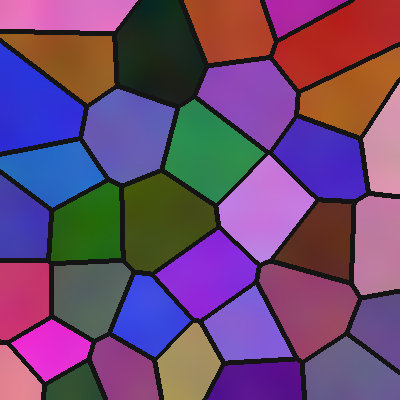
\includegraphics[width=36mm]{assets/drawn/grain-map}};
  \draw[white,line width=0.6pt] (map.south west) rectangle (map.north east);
  \draw[white,line width=0.9pt,-{Stealth[length=2mm,width=1.6mm]}] (131.5,-50.5) -- (131.5,-57);
  % the plane: 36 x 22 mm, yield strength 340-1000 MPa, elongation 30-86 %
  \begin{scope}[shift={(113.5,-83)}]
    \draw[white,line width=0.7pt] (0,22) -- (0,0) -- (36,0);
    \begin{scope}[x=0.054545mm,y=0.392857mm,shift={(-340,-30)}]
      \drawfront[white!75!udsblue,line width=0.6pt,dash pattern=on 1.4pt off 1pt]
      \foreach \s/\e/\i in \alloydata
        \node[circle,fill=white!85!udsblue,inner sep=0pt,minimum size=1.1mm] at (\s,\e) {};
      \node[circle,fill=white,inner sep=0pt,minimum size=4.6mm] (star) at (790,64) {};
      \node[text=udsred,font=\footnotesize] at (star) {\faStar};
    \end{scope}
  \end{scope}
  \fill[udsred] (102,1) rectangle (103.6,-91);}

% \doiline: https://doi.org/ and the paper's DOI, as a link in the slides; in the speaker notes, whose
% thumbnails scale the slide but not its links, the same text without a link
\newcommand\audiencemode{hide notes}
\ifx\notesmode\audiencemode
  \newcommand\doiline{\href{https://doi.org/\paperdoi}{https://doi.org/\paperdoi}}
\else
  \newcommand\doiline{\textcolor{udsblue}{https://doi.org/\paperdoi}}
\fi

% ------------------------------------------------------------------ title
\begin{frame}[plain,noframenumbering]
% Drawn inside the frame rather than over the page, so the speaker notes' thumbnail shows it too.
% The picture's origin is the page's top-left corner: a plain frame's body starts 8 mm in and
% 2 mm down.
\vbox to 0pt{\vskip-2mm\hbox to 0pt{\hskip-8mm\begin{tikzpicture}[x=1mm,y=1mm]
  \useasboundingbox (0,0) rectangle (160,-90);
  \titlepanel
  \node[anchor=north west,inner sep=0pt] at (8,-8) {\includegraphics[width=30mm]{\udslogo}};
  % the text block grows upwards from the presenter's name, whose baseline stays 66.5 mm from the top,
  % at the same distance from the d3M block as in the Coding Agents talk; the citation and the DOI under
  % it form one block, and the red rule sits halfway between that block and the name
  \node[anchor=south west,inner sep=0pt,text width=90mm,align=left,
    execute at begin node={\hyphenpenalty=10000\exhyphenpenalty=10000}] at (8,-66.63) {%
    {\fontsize{16.5}{18}\selectfont\bfseries\color{udsblue}\inserttitle\par}\vskip2mm
    {\fontsize{12}{14.5}\selectfont\color{udsdark}\insertsubtitle\par}\vskip0.6mm
    {\fontsize{9}{11}\selectfont\doiline\par}\vskip1.25mm
    \textcolor{udsred}{\rule{14mm}{0.8pt}}\par\vskip3mm
    {\fontsize{11}{13}\selectfont\color{udsdark}\insertauthor\par}};
  \node[anchor=south west,inner sep=0pt] (d3m) at (8,-83) {
\includegraphics[width=10mm]{assets/d3m.png}};
  \node[anchor=west,inner sep=0pt,text width=74mm,align=left,font=\fontsize{7}{8.8}\selectfont,
    execute at begin node={\hyphenpenalty=10000}] at ([xshift=3mm]d3m.east) {%
    {\color{udsblue}\insertinstitute\par}
    {\color{udsgrey}\insertdate\par}};
\end{tikzpicture}\hss}\vss}
% a frame with no tall content drops out of the notes' thumbnail; this invisible strut keeps it
\par\rule{0pt}{80mm}
\note{\textbf{0:00--0:20}\par
    A paper from Nature Communications, published at the end of September 2026.\par
    The authors train generative models on electron backscatter diffraction (EBSD) maps of 25 variants of
      one alloy, and search them for microstructures that are both stronger and more ductile.\par
    I follow the paper's own story.}
\end{frame}

% ---------------------------------------------------------------- outline
\begin{frame}{Outline}
  % each section's title as on its divider, and the divider's question
  \small\renewcommand\arraystretch{1.4}\setlength\tabcolsep{4pt}
  \begin{tabularx}{\textwidth}{@{}>{\leavevmode\color{udsblue}\bfseries}p{4mm}>{\bfseries}p{42mm}X@{}}
    \toprule
    1 & The design problem   & Why ask a generative model for new microstructures?\\
    2 & Groundwork           & Which methods does the paper build on?\\
    3 & The method           & How are microstructures generated and steered toward properties?\\
    4 & The results          & What do the authors show?\\
    \bottomrule
  \end{tabularx}
  \note{\textbf{0:20--0:50}\par
    Four sections, each answering one question.\par
    Section 2 introduces the machine-learning methods the paper combines, with their origins, for anyone
      who has not followed that literature.\par
    Sections 3 and 4 present the paper as the authors tell it.}
\end{frame}

\section[Problem]{The design problem}
\sectionframe{01}{The design problem}{Why ask a generative model for new microstructures?}{\faBalanceScale}

% ------------------------------------------------------------ the trade-off
\begin{frame}[source={Liao et al.\ (2026), Nat.\ Commun.\ 17, 11232}]{Strength/ductility trade-off}
  \begin{tikzpicture}[x=1mm,y=1mm]
    \useasboundingbox (0,0) rectangle (144,-54);
    \begin{scope}[shift={(16,-42)}]
      \planeaxes{340}{1000}{28}{86}{124}{42}{400,500,...,1000}{30,40,...,80}
      \begin{scope}[plane]
        \drawfront[front]
        \drawalloys
        \draw[udsred,line width=1.1pt,-{Stealth[length=2.6mm,width=2mm]}] (640,55) -- (760,72);
        \node[anchor=west,inner sep=0pt,font=\footnotesize\bfseries,text=udsred] at (768,73.5)
          {goal: stronger and more ductile};
        % the two ends of the trade-off, each beside the axis it is close to
        \node[anchor=west,inner sep=0pt,font=\footnotesize\bfseries,text=udsdark] at (410,84) {ductile, but weak};
        \node[anchor=east,inner sep=0pt,font=\footnotesize\bfseries,text=udsdark] at (1000,41) {strong, but brittle};
        \node[anchor=west,label text] at (360,33) {25 alloys, one processing route each};
        \node[anchor=west,small label] (fl) at (600,40) {measured front};
        \draw[udsgreymid,line width=0.4pt] (fl.north east) -- (700.46,45);
      \end{scope}
    \end{scope}
    \node[axis label] at (78,-49.4) {yield strength (MPa)};
    \node[axis label,rotate=90] at (3,-21) {elongation (\%)};
  \end{tikzpicture}
  \note{\textbf{1:00--2:10}\par
    Each point is one alloy: Inconel 625, a nickel-based superalloy used for turbine discs, blades and
      combustors, processed in one of 25 ways.\par
    The alloys differ only in processing: hot rolling and annealing at different temperatures and
      times.\par
    Each was tensile-tested for its yield strength and its elongation to failure.\par
    The stronger variants stretch less: a strength--ductility trade-off; making a metal stronger
      usually makes it brittle, and making it ductile makes it weak.\par
    The dashed staircase is the front: no measured alloy beats a point on it in both properties.\par
    The goal is a microstructure above and to the right of the front.\par
    Such microstructures are usually found by experience and trial and error over processing
      routes; the paper asks a generative model to propose them.}
\end{frame}

% ------------------------------------------------------- failure case
\begin{frame}[source={Liao et al.\ (2026), Nat.\ Commun.\ 17, 11232, Fig.\ 2c (CC BY-NC-ND 4.0)}]
  {Classic pixelwise loss fails}
  \begin{tikzpicture}[x=1mm,y=1mm]
    \useasboundingbox (0,0) rectangle (144,-54);
    \figpart{32}{0}{2}{340}{770}{1897}{1268}{112}
    \node[anchor=east,label text,align=right] at (29,{\fpy{884}}) {real patches};
    \node[anchor=east,label text,align=right,text=udsred] (pl) at (29,{\fpy{1155}}) {pixel loss only};
    % the two classic pixel losses over the n pixels of a patch x and its reconstruction
    \node[anchor=north east,inner sep=0pt,font=\scriptsize,text=udsdark,align=right] at ([yshift=-1.6mm]pl.south east)
      {MAE $=\frac{1}{n}\sum_i|x_i-\hat{x}_i|$\\[1.2mm] MSE $=\frac{1}{n}\sum_i(x_i-\hat{x}_i)^2$};
    \warnstrip{-41.4}{blurred or missing grain boundaries, colours mixed inside grains}
  \end{tikzpicture}
  \note{\textbf{2:10--3:10}\par
    These are real patches of 50 by 50 micrometres from test alloys, cut from EBSD maps.\par
    In an EBSD map each pixel's colour encodes the crystal orientation there: the three Euler angles
      as red, green and blue; the black lines are grain boundaries.\par
    The second row is what the paper's generator returns when it is trained to reproduce its input
      with a pixel loss alone, the mean absolute difference of the pixel values (MAE); the mean squared
      difference (MSE) is the other classic choice, and both average over all pixels.\par
    The boundaries blur, and colours mix inside grains, although a real grain has nearly one
      orientation.\par
    Boundaries cover few pixels, so an average over all pixels barely notices them; yet boundaries
      and orientations are what set the mechanical properties.}
\end{frame}

% ------------------------------------------------------------- the idea
\begin{frame}[source={Liao et al.\ (2026), Nat.\ Commun.\ 17, 11232, after Figs.\ 1 and 4f}]{Two fixes}
  \begin{tikzpicture}[x=1mm,y=1mm]
    \useasboundingbox (0,0) rectangle (144,-54);
    \tikzset{verdict mark/.style={circle,text=white,inner sep=0pt,minimum size=3.8mm,font=\scriptsize},
      head/.style={anchor=west,inner sep=0pt,font=\footnotesize\bfseries},
      panel title/.style={anchor=north west,inner sep=0pt,font=\footnotesize\bfseries,text=udsdark},
      note/.style={anchor=north west,label text,text width=22mm}}
    % column heads: what goes wrong, and what the paper changes
    \node[verdict mark,fill=udsred] (bad) at (1.9,-1.9) {\faTimes};
    \node[head,text=udsred] at ([xshift=1.6mm]bad.east) {the obstacle};
    \node[verdict mark,fill=testgreen] (good) at (87.9,-1.9) {\faCheck};
    \node[head,text=testgreen] at ([xshift=1.6mm]good.east) {the paper's fix};
    % row 1, the loss: the same patch region, three times enlarged, before and after
    \fill[redtint] (0,-5.6) rectangle (58,-28.4);
    \fill[greentint] (86,-5.6) rectangle (144,-28.4);
    \node[panel title] at (2.4,-7.4) {$L=L_{\mathrm{pix}}$};
    \node[panel title] at (88.4,-7.4) {$L=L_{\mathrm{pix}}+\textcolor{testgreen}{L_{\mathrm{edge}}+L_{\mathrm{SSIM}}}$};
    \foreach \x/\img in {2.4/grain-map-blurred,88.4/grain-map} {
      \node[anchor=north west,inner sep=0pt] at (\x,-12.6) {\includegraphics[width=14mm]{assets/drawn/\img}};
      \draw[udsdark,line width=0.4pt] ({\x+4.9},-17.5) rectangle ++(4.2,-4.2);
      \begin{scope}
        \clip ({\x+24},-19.6) circle (6.3);
        \node[anchor=north west,inner sep=0pt] at ({\x+3},1.4) {\includegraphics[width=42mm]{assets/drawn/\img}};
      \end{scope}
      \draw[udsdark,line width=0.5pt] ({\x+24},-19.6) circle (6.3);
      \draw[udsdark,line width=0.3pt] ({\x+9.1},-17.5) -- ({\x+19.6},-15.1) ({\x+9.1},-21.7) -- ({\x+19.6},-24.1);}
    \node[note] at (121.4,-13.4) {sharp boundaries, one colour per grain};
    \fixarrow{60.4}{83.6}{-17}{more terms}
    % row 2, the sampling: the latent space sampled at random, and searched toward targets (after Fig. 1c)
    \fill[redtint] (0,-31.2) rectangle (58,-54);
    \fill[greentint] (86,-31.2) rectangle (144,-54);
    \node[panel title] at (2.4,-33) {random sampling};
    \node[panel title] at (88.4,-33) {property-guided search};
    \tikzset{code/.style={circle,fill=udsgreymid,inner sep=0pt,minimum size=1.3mm},
      new code/.style={circle,fill=udsblue,inner sep=0pt,minimum size=1.5mm},
      latent/.style={fill=white,draw=udsgreylight,line width=0.4pt}}
    % left: codes drawn at random fall among the training codes
    \filldraw[latent] (14,-43.6) ellipse (10 and 7);
    \foreach \x/\y in {9.6/-38.6,7/-41.4,5.8/-43.8,8.4/-45,9.8/-48.4,14.6/-38.4,19.6/-39,18.6/-48.2,14.8/-49.2}
      \node[code] at (\x,\y) {};
    \node[anchor=north,small label] at (14,-51.2) {latent space};
    % the three new codes join, and one arrow goes on to the sentence about them; the training codes
    % leave each line a clear path
    \node[note,text width=27mm,anchor=west] at (28.4,-43.6) {new codes fall among the training codes};
    \foreach \x/\y in {12/-40.4,15.8/-43.6,11.2/-47}
      \draw[udsblue,line width=0.5pt,shorten <=1mm] (\x,\y) to[out=0,in=180] (22.4,-43.6);
    \draw[udsblue,line width=0.5pt,-{Stealth[length=1.5mm,width=1.1mm]}] (22.4,-43.6) -- (27.4,-43.6);
    \foreach \x/\y in {12/-40.4,15.8/-43.6,11.2/-47} \node[new code] at (\x,\y) {};
    % right: the search steers codes to targets outside them, beyond the measured front (after Fig. 1c)
    \filldraw[latent] (97.6,-45) ellipse (8 and 5.8);
    \foreach \x/\y in {-4.6/1.4,-2/-2.4,0.4/2.6,2.2/-0.6,4.6/1.6,-0.6/-4,5/-2.6,-5.4/-1.2}
      \node[code] at (97.6+\x,-45+\y) {};
    \draw[udsblue,line width=0.9pt,-{Stealth[length=1.8mm,width=1.4mm]}] (104.8,-42.6) -- (107.9,-41.4);
    \filldraw[fill=udsblue!22,draw=udsblue,line width=0.4pt] (111.2,-40.6) circle (3.2);
    \foreach \x/\y in {-1.2/0.9,1.2/-0.9} \node[text=udsred,font=\tiny] at (111.2+\x,-40.6+\y) {\faStar};
    \node[anchor=north,small label] at (97.6,-51.2) {latent space};
    \node[anchor=north,small label] at (111.2,-44.2) {targets};
    \begin{scope}[shift={(119,-49.4)}]
      \draw[udsgreymid,line width=0.5pt] (0,11.4) -- (0,0) -- (22,0);
      \node[anchor=north,small label] at (11,-0.6) {strength};
      \node[anchor=south,small label,rotate=90] at (-0.6,5.7) {elongation};
      \begin{scope}[x=0.033333mm,y=0.203571mm,shift={(-340,-30)}]
        \drawfront[front]
        \drawalloys[minimum size=1mm]
        \draw[udsred,line width=0.7pt,-{Stealth[length=1.6mm,width=1.2mm]}] (600,51) -- (660,61);
        \drawcandidates[minimum size=1.3mm]
      \end{scope}
    \end{scope}
    \fixarrow{60.4}{83.6}{-42.2}{steer by properties}
  \end{tikzpicture}
  \note{\textbf{3:10--4:10}\par
    The paper answers two obstacles with two changes: the obstacles on the left, its fixes on the
      right.\par
    First, a pixel loss alone blurs grain boundaries, as the enlarged region shows; the paper adds two
      terms, one that responds to grain boundaries and one to the structure inside grains.\par
    Second, codes drawn at random from the model's latent space fall among the training codes, so the new
      samples resemble the measured alloys.\par
    So the authors search the latent space, steered by predicted strength and ductility, toward targets
      outside the training codes, as their Fig.~1c sketches; their five candidates lie beyond the measured
      front.\par
    Section 2 explains the models and the search for anyone who has not met them.}
\end{frame}

\section[Groundwork]{Groundwork}
\sectionframe{02}{Groundwork}{Which methods does the paper build on?}{\faBookOpen}

% ----------------------------------------------------- three ways to generate
\begin{frame}[source={Kingma and Welling (2013), arXiv:1312.6114 · Goodfellow et al.\ (2014), NeurIPS · Ramesh et al.\ (2021), ICML · Ho et al.\ (2020), NeurIPS · Rombach et al.\ (2022), CVPR}]
  {Three ways to generate an image}
  \begin{tikzpicture}[x=1mm,y=1mm]
    \useasboundingbox (0,0) rectangle (144,-54);
    \foreach \i/\c/\h in {0/udsblue/In one pass,1/udsgreymid/Token by token,2/udsblue/Step by step from noise} {
      \pgfmathsetmacro\cx{\i*49}
      \fill[\c!8] (\cx,-5.4) rectangle ++(46,-41.6);
      \cardhead{\cx}{0}{46}{\c}{\h}
    }
    % in one pass: a code, decoded into the whole image
    \filldraw[fill=udsblue,draw=udsblue] (6,-12.3) rectangle (10.4,-19.7);
    \node[text=white,font=\small\itshape,inner sep=0pt] at (8.2,-16) {z};
    \draw[flow] (11,-16) -- (14.2,-16);
    \filldraw[fill=bluetint,draw=udsblue,line width=0.5pt] (15,-12.5) -- (25.4,-9) -- (25.4,-23) -- (15,-19.5) -- cycle;
    \node[label text,rotate=90] at (20.2,-16) {decoder};
    \draw[flow] (26,-16) -- (29.2,-16);
    \node[anchor=north west,inner sep=0pt] at (30,-9.5) {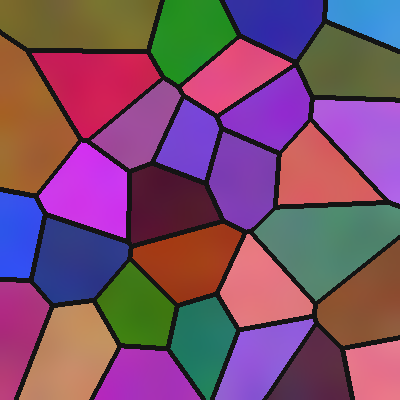
\includegraphics[width=13mm]{assets/drawn/grain-map-new}};
    % token by token: tiles written in reading order, the next one outlined
    \node[anchor=north west,inner sep=0pt] at (65,-9) {
\includegraphics[width=14mm]{assets/drawn/tokens-partial}};
    \begin{scope}[shift={(65,-23)}]
      \draw[udsgreylight,line width=0.3pt] (0,0) grid[step=1.75] (14,14);
      \draw[udsred,line width=0.8pt] (5.25,7) rectangle (7,8.75);
    \end{scope}
    % step by step from noise: the whole image refined at every step
    \foreach \t/\x in {1000/100.5,150/116,0/131.5}
      \node[anchor=north west,inner sep=0pt] at (\x,-10.5) {\includegraphics[width=11mm]{assets/drawn/diffusion-t\t}};
    \draw[flow,draw=udsblue] (112,-16) -- (115.4,-16);
    \draw[flow,draw=udsblue] (127.5,-16) -- (130.9,-16);
    % what each does, examples, and how the image is built
    \foreach \i/\a/\e/\b in {0/{a decoder turns a code into an image}/{VAE (2013), GAN (2014)}/{whole image at once},
        1/{a network predicts each tile from the tiles before it}/{DALL-E 1 (2021); language models write text
          this way}/{no going back to refine},
        2/{a network removes a little noise at each step}/{DDPM (2020), Stable Diffusion (2022), DALL-E 2
          (2022)}/{refines the whole image}} {
      \node[card text,text width=42mm] at ({\i*49+2},-26.6) {\a};
      \node[card text,text width=42mm,font=\scriptsize,text=udsgrey] at ({\i*49+2},-35) {\e};
      \node[card text,text width=42mm,font=\footnotesize\bfseries] at ({\i*49+2},-42.4) {\b};}
    \node[anchor=north west,small label,text=udsred] at (0,-49.4)
      {Liao et al.\ join the first and the third: the VAE output guides the diffusion steps};
  \end{tikzpicture}
  \note{\textbf{4:20--5:20}\par
    Generative models differ in how they build an image.\par
    In one pass: a decoder turns a short code into the whole image at once; VAEs and GANs work this
      way.\par
    Token by token: a network predicts each piece of the image from the pieces before it, as language
      models write text word by word; DALL-E 1 (Ramesh and colleagues, 2021) wrote 32 by 32 such tokens,
      which a discrete VAE then decoded into the image.\par
    Such a model starts from scratch and works in a fixed order, so it cannot go back and refine what it
      has written.\par
    Step by step from noise: a diffusion model starts from noise and refines the whole image at every
      step; Stable Diffusion and DALL-E 2 and 3 work this way, and diffusion leads image generation
      today.\par
    The paper joins the first and the third: a VAE generates in one pass, and its output guides the
      diffusion steps.}
\end{frame}

% ------------------------------------------------------------------ VAE
\begin{frame}[source={Kingma and Welling (2013), arXiv:1312.6114}]{Variational Autoencoder (VAE)}
  \begin{tikzpicture}[x=1mm,y=1mm]
    \useasboundingbox (0,0) rectangle (144,-54);
    \tikzset{part/.style={fill=bluetint,draw=udsblue,line width=0.5pt}}
    % encode, sample, decode; the row's centre line is y = -11.5
    \node[anchor=north west,inner sep=0pt] at (0,-5.5) {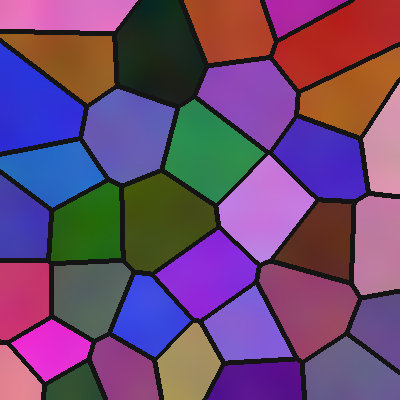
\includegraphics[width=12mm]{assets/drawn/grain-map}};
    \node[anchor=north,small label,text=udsdark] at (6,-18.4) {patch};
    \draw[flow] (12.6,-11.5) -- (16.6,-11.5);
    \filldraw[part] (17.4,-4) -- (27.8,-7.5) -- (27.8,-15.5) -- (17.4,-19) -- cycle;
    \node[label text,rotate=90] at (22.6,-11.5) {encoder};
    \draw[flow] (28.4,-11.5) -- (31.4,-11.5);
    \filldraw[fill=bluetint,draw=udsblue,line width=0.5pt] (32,-6.8) rectangle (36,-11.1);
    \filldraw[fill=darktint,draw=udsdark,line width=0.5pt] (32,-11.9) rectangle (36,-16.2);
    \node[font=\scriptsize,inner sep=0pt,text=udsdark] at (34,-8.95) {$\mu$};
    \node[font=\scriptsize,inner sep=0pt,text=udsdark] at (34,-14.05) {$\sigma$};
    \node[anchor=north,small label,text=udsdark,align=center] at (34,-18.4) {mean,\\ spread};
    \draw[flow] (36.6,-11.5) -- (39.6,-11.5);
    % sample: a normal curve with one drawn value
    \draw[udsgreymid,line width=0.4pt] (40.4,-14.5) -- (49.6,-14.5);
    \draw[udsblue,line width=0.7pt] plot[domain=-2.6:2.6,samples=41] ({45+\x*1.75},{-14.5+6.5*exp(-((\x)^2)/2)});
    \node[circle,fill=udsred,inner sep=0pt,minimum size=1.5mm] at (46.6,-14.5) {};
    \node[anchor=north,small label,text=udsdark] at (45,-18.4) {sample $z$};
    \draw[flow] (50.2,-11.5) -- (53.2,-11.5);
    \filldraw[part] (54,-7.5) -- (64.4,-4) -- (64.4,-19) -- (54,-15.5) -- cycle;
    \node[label text,rotate=90] at (59.2,-11.5) {decoder};
    \draw[flow] (65,-11.5) -- (69,-11.5);
    \node[anchor=north west,inner sep=0pt] at (69.6,-5.5) {
\includegraphics[width=12mm]{assets/drawn/grain-map-blurred}};
    \node[anchor=north,small label,text=udsdark] at (75.6,-18.4) {reconstruction};
    % the loss, each term labelled
    \node[font=\large,text=udsdark,inner sep=0pt] at (4,-32) {$L\;=$};
    \node[font=\large,text=udsdark,inner sep=0pt] (rec) at (21,-32) {$L_{\mathrm{rec}}$};
    \node[font=\large,text=udsdark,inner sep=0pt] at (41,-32) {$+$};
    \node[font=\large,text=udsblue,inner sep=0pt] (kl) at (62,-32) {$L_{\mathrm{KL}}$};
    \node[anchor=north,label text,align=center,text width=28mm] at (21,-36.4) {output close\\ to the input};
    \node[anchor=north,label text,align=center,text width=28mm,text=udsblue] at (62,-36.4)
      {codes close to\\ a standard normal};
    % the latent space: each patch's code is a small cloud, and the clouds overlap
    \draw[udsgreymid,line width=0.5pt] (92,0) rectangle (144,-44);
    \node[anchor=north west,small label] at (93.4,-1.4) {latent space, 2 of 128 directions};
    \foreach \x/\y in {104/-24,110/-18,111/-29,117/-23,103/-33,118/-33,124/-27,109/-38,98/-28}
      {\fill[udsblue,fill opacity=0.14] (\x,\y) circle (4.4); \fill[udsblue] (\x,\y) circle (0.55);}
    \node[text=udsred,font=\footnotesize,inner sep=0pt] (new) at (114.2,-24.4) {\faStar};
    \node[anchor=north west,inner sep=0pt] (np) at (129.4,-9.4) {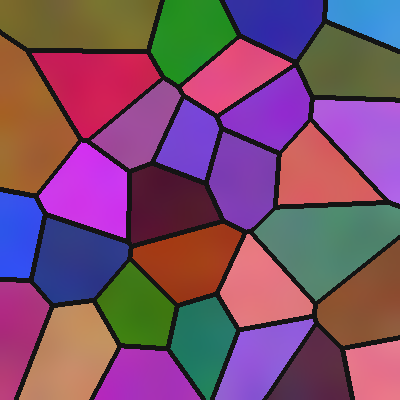
\includegraphics[width=11mm]{assets/drawn/grain-map-new}};
    \draw[udsred,line width=0.7pt,-{Stealth[length=1.6mm,width=1.2mm]}] (new.north east) to[out=40,in=200] (np.west);
    \node[anchor=north,small label,text=udsred,align=center] at (134.9,-21.2) {new code,\\ new patch};
  \end{tikzpicture}
  \note{\textbf{5:20--6:40}\par
    An autoencoder is a network trained to copy its input through a bottleneck: an encoder compresses the
      image into a few numbers, the latent code, and a decoder rebuilds the image from them.\par
    The variational autoencoder, from Kingma and Welling in 2013, makes the code probabilistic: the
      encoder gives a mean and a spread for each number, and the decoder sees a value drawn from that
      range.\par
    A Kullback--Leibler (KL) term pulls every code towards a standard normal distribution, so the codes
      of different images overlap and the space has no gaps.\par
    That makes a VAE generative: a code drawn from this space decodes to a plausible image, and moving
      through the space changes the image smoothly.\par
    Trained with a pixel loss, a VAE returns blurry images, the average of the plausible answers: the
      failure of slide 3.\par
    In this paper each patch gets a code of 128 numbers.}
\end{frame}

% ----------------------------------------------- reconstruct, generate, extrapolate
\begin{frame}{Reconstruct, generate, extrapolate}
  \begin{tikzpicture}[x=1mm,y=1mm]
    \useasboundingbox (0,0) rectangle (144,-54);
    \tikzset{code/.style={circle,fill=udsgreymid,inner sep=0pt,minimum size=1.2mm}}
    \foreach \i/\c/\h in {0/udsdark/Reconstruct,1/udsblue/Generate,2/udsred/Extrapolate} {
      \pgfmathsetmacro\cx{\i*49}
      \fill[\c!8] (\cx,-5.4) rectangle ++(46,-41.6);
      \cardhead{\cx}{0}{46}{\c}{\h}
      % the training codes, the same cloud in every card
      \begin{scope}[shift={(\cx,0)}]
        \filldraw[fill=white,draw=udsgreylight,line width=0.5pt] (21,-16.5) ellipse (8.6 and 5.6);
        \foreach \x/\y in {16/-15,18.6/-19,20.4/-13.6,22.6/-17.4,24.8/-14.6,26.2/-18.4,15.4/-17.8,19.4/-16.2}
          \node[code] at (\x,\y) {};
      \end{scope}
    }
    % reconstruct: a training patch, encoded and decoded
    \node[anchor=north west,inner sep=0pt] (in) at (1.4,-11.5) {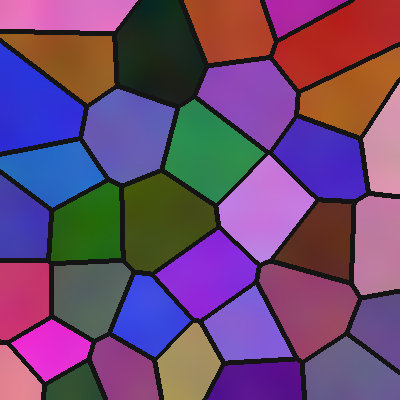
\includegraphics[width=10mm]{assets/drawn/grain-map}};
    \node[circle,draw=udsdark,line width=0.7pt,inner sep=0pt,minimum size=2.6mm] (c0) at (22.6,-17.4) {};
    \draw[flow,line width=0.5pt] (in.east) to[out=0,in=180] (c0.west);
    \node[anchor=north west,inner sep=0pt] (out0) at (34.6,-11.5) {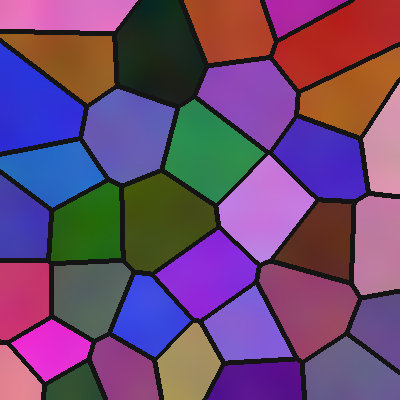
\includegraphics[width=10mm]{assets/drawn/grain-map}};
    \draw[flow,line width=0.5pt] (c0.east) to[out=0,in=180] (out0.west);
    % generate: a new code among the training codes
    \node[circle,fill=udsblue,inner sep=0pt,minimum size=2mm] (c1) at (49+23.4,-15.6) {};
    \node[anchor=north west,inner sep=0pt] (out1) at (49+34.6,-11.5) {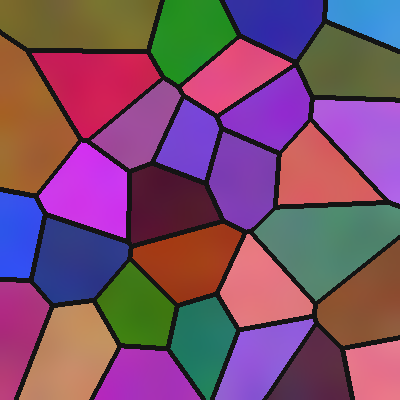
\includegraphics[width=10mm]{assets/drawn/grain-map-new}};
    \draw[flow,draw=udsblue,line width=0.5pt] (c1.east) to[out=0,in=180] (out1.west);
    % extrapolate: a code away from every training code
    \node[text=udsred,font=\footnotesize,inner sep=0pt] (c2) at (98+31.4,-25.4) {\faStar};
    \node[anchor=north west,inner sep=0pt] (out2) at (98+34.6,-11.5) {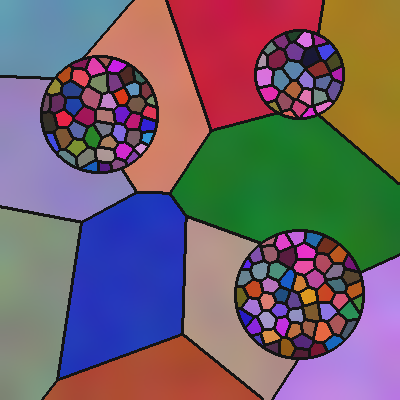
\includegraphics[width=10mm]{assets/drawn/grain-map-bimodal}};
    \node[circle,fill=white,draw=udsred,line width=0.6pt,inner sep=0pt,minimum size=4.2mm,font=\scriptsize\bfseries,
      text=udsred] at ([xshift=-1mm,yshift=1mm]out2.north east) {?};
    \draw[flow,draw=udsred,line width=0.5pt] (c2.east) to[out=0,in=-90] (out2.south);
    % what each is, and what can check it
    \foreach \i/\a/\b in {0/{a training patch, encoded and decoded}/{compare with its input},
        1/{a new code among the training codes}/{compare with held-out data},
        2/{a code away from all training codes}/{only an experiment can tell}} {
      \node[anchor=north west,card text,text width=42mm] at ({\i*49+2},-29.4) {\a};
      \node[anchor=north west,card text,text width=42mm,font=\footnotesize\bfseries] at ({\i*49+2},-41.4) {\b};}
  \end{tikzpicture}
  \note{\textbf{6:40--7:40}\par
    A trained generative model can do three different things, and each needs a different check.\par
    Reconstruct: encode a training patch and decode it again; the result can be compared with its own
      input, pixel by pixel or by its statistics.\par
    Generate: decode a new code from among the training codes; the result has no original, so it is
      compared with the statistics of held-out data and checked for near-copies of training patches.\par
    Extrapolate: decode a code away from all training codes; no example lies there, so only an
      experiment can tell whether the result is realistic.\par
    The paper claims all three; the results show what each claim rests on.}
\end{frame}

% ------------------------------------------------------------ diffusion
\begin{frame}[source={Sohl-Dickstein et al.\ (2015), ICML · Ho et al.\ (2020), NeurIPS · Ronneberger et al.\ (2015), MICCAI}]
  {Diffusion models}
  \begin{tikzpicture}[x=1mm,y=1mm]
    \useasboundingbox (0,0) rectangle (144,-54);
    \node[anchor=north west,label text,text=udsgrey] (fwd) at (0,0)
      {forward: at each of 1000 steps, mix in a little noise\enspace\textcolor{udsgreymid}{(fixed)}};
    \node[anchor=base east,label text] at (fwd.base -| 144,0) {$x_t=\sqrt{1-\beta_t}\,x_{t-1}+\sqrt{\beta_t}\,\epsilon$};
    \foreach \t [count=\i from 0] in {0,50,150,300,1000} {
      \node[anchor=north west,inner sep=0pt] (d\i) at ({2+29*\i},-6.6) {\includegraphics[width=18mm]{assets/drawn/diffusion-t\t}};
      \node[anchor=north,small label,text=udsdark] at ({11+29*\i},-25.4) {$t=\t$};}
    \foreach \i in {0,...,3} {
      \draw[flow,draw=udsgreymid] ({20.6+29*\i},-11.6) -- ({30.4+29*\i},-11.6);
      \draw[flow,draw=udsblue] ({30.4+29*\i},-19.6) -- ({20.6+29*\i},-19.6);}
    \node[anchor=north west,label text,text=udsblue] at (0,-30.4)
      {reverse: a U-Net predicts the noise, removed step by step\enspace\textcolor{udsblue!70}{(learned)}};
    % generating with the trained model, two ways: from noise alone, or from noise and a guide (the paper)
    \tikzset{step image/.style={anchor=west,inner sep=0pt},
      way name/.style={anchor=west,inner sep=0pt,font=\footnotesize\bfseries,text=udsdark},
      way text/.style={card text,anchor=west,text width=84mm}}
    \node[anchor=north west,label text,text=udsgrey] at (0,-34.4) {generating with the trained model, two ways:};
    \foreach \y in {-41.6,-49.8} \fill[bluetint] (0,\y+3.9) rectangle (144,\y-3.9);
    % unconditional: noise alone
    \node[way name] at (2.4,-41.6) {unconditional};
    \node[step image] (u0) at (27,-41.6) {
\includegraphics[width=6.6mm]{assets/drawn/diffusion-t1000}};
    \node[step image] (u1) at (49.4,-41.6) {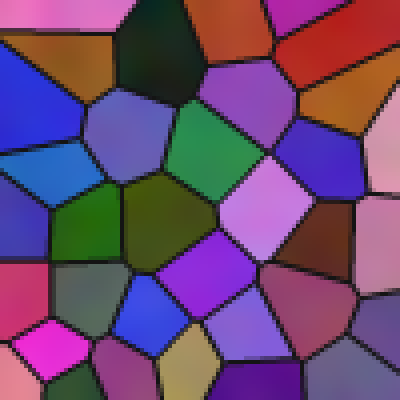
\includegraphics[width=6.6mm]{assets/drawn/diffusion-t0}};
    \draw[flow,draw=udsblue] ([xshift=0.6mm]u0.east) -- ([xshift=-0.6mm]u1.west);
    \node[way text] at (59,-41.6) {from noise alone, step by step: a new patch of any kind};
    % conditional: noise and a guide image
    \node[way name] at (2.4,-49.8) {conditional};
    \node[step image] (c0) at (27,-49.8) {
\includegraphics[width=6.6mm]{assets/drawn/diffusion-t1000}};
    \node[font=\small\bfseries,text=udsdark,inner sep=0pt] at (35.4,-49.8) {+};
    \node[step image] (c1) at (37.2,-49.8) {
\includegraphics[width=6.6mm]{assets/drawn/grain-map-blurred}};
    \draw[udsred,line width=0.6pt] (c1.south west) rectangle (c1.north east);
    \node[step image] (c2) at (49.4,-49.8) {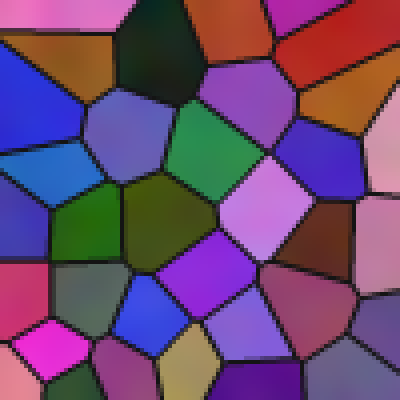
\includegraphics[width=6.6mm]{assets/drawn/diffusion-t0}};
    \draw[flow,draw=udsblue] ([xshift=0.6mm]c1.east) -- ([xshift=-0.6mm]c2.west);
    \node[way text] at (59,-49.8) {the U-Net also sees a \textcolor{udsred}{guide} at every step, here the VAE
      output};
  \end{tikzpicture}
  \note{\textbf{7:40--8:50}\par
    A diffusion model learns to undo noise.\par
    The forward process is fixed: each of 1000 steps scales the image down slightly and adds a little
      Gaussian noise $\epsilon$, with $\beta_t$ rising from 0.0001 to 0.02; after a few hundred steps only
      noise is left.\par
    Each step depends only on the one before, a Markov chain; the paper writes it as a Gaussian, its
      Eq.~12.\par
    The reverse process is learned: a network predicts the noise in an image at any step, and removing it
      step by step runs the process backwards.\par
    The idea is from Sohl-Dickstein and colleagues, 2015; DDPM, from Ho, Jain and Abbeel in 2020, made
      the images sharp.\par
    Once trained, it generates in two ways: from noise alone, any new patch; or with a guide image that
      the U-Net sees at every step, a patch that follows the guide.\par
    The paper's guide is the VAE's blurry output, so the diffusion model only restores detail; the next
      slide shows the training.}
\end{frame}

% ---------------------------------------------------- training a diffusion model
\begin{frame}[source={Ho et al.\ (2020), NeurIPS · Ronneberger et al.\ (2015), MICCAI}]
  {Training a diffusion model}
  \begin{tikzpicture}[x=1mm,y=1mm]
    \useasboundingbox (0,0) rectangle (144,-54);
    \begin{scope}[yshift=1mm]% content starts 4 mm below the title
    % a patch and a noise image, mixed in one go to a random step t
    \node[anchor=north west,inner sep=0pt] (x0) at (0,-1) {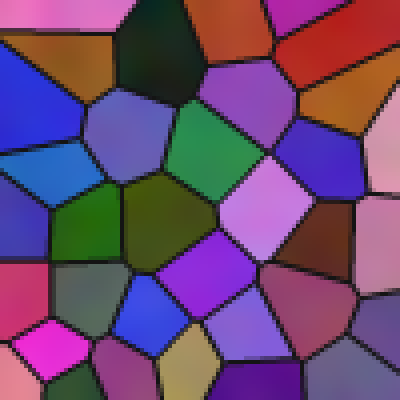
\includegraphics[width=12mm]{assets/drawn/diffusion-t0}};
    \node[anchor=north,small label,text=udsdark] at (6,-13.8) {patch $x_0$};
    \node[anchor=north west,inner sep=0pt] (eps) at (0,-21) {
\includegraphics[width=12mm]{assets/drawn/diffusion-noise}};
    \node[anchor=north,small label,text=udsdark] at (6,-33.8) {noise $\epsilon$};
    \node[draw=udsgreymid,fill=darktint,line width=0.5pt,inner sep=1.6mm,align=center,font=\footnotesize,
      text=udsdark] (mix) at (39,-7)
      {{\scriptsize\color{udsgrey}a random step $t$, in one go}\\[0.6mm]
       $x_t=\sqrt{\bar\alpha_t}\,x_0+\sqrt{1-\bar\alpha_t}\,\epsilon$};
    \draw[flow] (x0.east) -- (x0.east -| mix.west);
    \draw[flow] (12,-24) to[out=0,in=-90] (30,-12.6 |- mix.south);
    % the noised patch and its step go into the U-Net, which predicts the noise
    \node[anchor=north west,inner sep=0pt] (xt) at (66,-1) {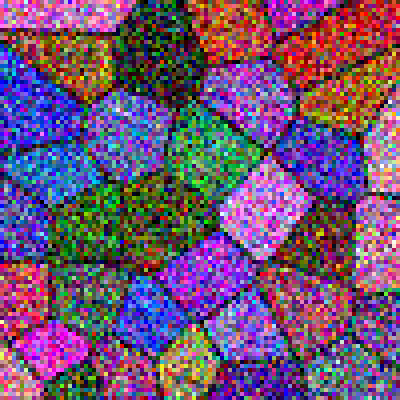
\includegraphics[width=12mm]{assets/drawn/diffusion-t150}};
    \node[anchor=north,small label,text=udsdark] at (72,-13.8) {$x_t$, here $t=150$};
    \draw[flow] (mix.east) -- (mix.east -| xt.west);
    \node[draw=udsblue,fill=bluetint,line width=0.5pt,minimum width=14mm,minimum height=9mm,font=\footnotesize,
      text=udsblue,inner sep=0pt] (unet) at (92,-7) {U-Net};
    \draw[flow] (xt.east |- unet.west) -- (unet.west);
    \node[anchor=north,small label,text=udsdark] (tin) at (92,-17.4) {step $t$};
    \draw[flow,line width=0.5pt] (tin.north) -- (unet.south);
    \node[anchor=west,font=\footnotesize,text=udsblue,inner sep=0pt] (pred) at (105.2,-7) {$\epsilon_\theta(x_t,t)$};
    \node[anchor=north,small label,text=udsblue] at ([yshift=-1.4mm]pred.south) {predicted noise};
    \draw[flow] (unet.east) -- (pred.west);
    % the loss: the predicted noise against the noise that was added
    \node[draw=udsred,fill=redtint,line width=0.5pt,inner sep=1.6mm,font=\footnotesize,text=udsdark] (loss)
      at (pred.center |- 0,-29) {$\|\epsilon-\epsilon_\theta(x_t,t)\|^2$};
    \draw[flow] ([yshift=-5.6mm]pred.south) -- (loss.north);
    \draw[flow,draw=udsred] (eps.east |- loss.west) -- (loss.west);
    \node[anchor=south,small label,text=udsred] at (56,-28.4) {the noise that was added is the target};
    \node[anchor=west,small label,text width=14mm] at ([xshift=1.6mm]loss.east) {loss: trains the U-Net};
    \end{scope}
    % repeated over many patches; the paper adds the VAE output as an input
    \fill[bluetint] (0,-40.4) rectangle (70,-53.6);
    \node[card text,anchor=west,text width=66mm] at (2,-47) {repeated over many patches, steps and noise
      images: one U-Net learns all 1000 steps};
    \fill[redtint] (74,-40.4) rectangle (144,-53.6);
    \node[card text,anchor=west,text width=66mm] at (76,-47) {Liao et al.: the U-Net also sees the VAE output,
      $\epsilon_\theta(x_t,t,x_V)$};
  \end{tikzpicture}
  \note{\textbf{8:50--10:00}\par
    A diffusion model is trained on one simple task: predict the noise in a noised image.\par
    Take a training patch $x_0$, draw a noise image $\epsilon$ and a random step $t$, and mix them in one
      go; $\bar\alpha_t$, the product of all $1-\beta_s$ up to step $t$, says how much of the patch is
      left.\par
    The network, a U-Net (Ronneberger and colleagues, 2015), gets the noised patch and the step and returns
      a noise image of the same size.\par
    The loss is the squared error between the added and the predicted noise; repeated over many patches,
      steps and noise images, one network learns every step.\par
    Knowing the noise is enough to step back: each reverse step subtracts a share of the predicted noise
      and adds a little fresh noise.\par
    The paper trains its diffusion model this way, with the VAE output $x_V$ as a third input, and
      compares the noise with the loss of section 3.}
\end{frame}

% --------------------------------------------------------- Pareto, NSGA-II
\begin{frame}[source={Pareto (1906), \emph{Manuale di economia politica} · Holland (1975), \emph{Adaptation in Natural and Artificial Systems} · Deb et al.\ (2002), IEEE Trans.\ Evol.\ Comput.\ 6, 182}]
  {Pareto fronts and NSGA-II}
  \begin{tikzpicture}[x=1mm,y=1mm]
    \useasboundingbox (0,0) rectangle (144,-54);
    \tikzset{panel frame/.style={draw=udsgreylight,line width=0.5pt,rounded corners=1mm},
      name part/.style={anchor=north,inner sep=0pt,font=\Large\bfseries,text=udsblue},
      name meaning/.style={anchor=north,small label,text=udsdark},
      front point/.style={circle,fill=udsblue,inner sep=0pt,minimum size=1.6mm},
      back point/.style={circle,fill=udsgreymid,inner sep=0pt,minimum size=1.6mm},
      point name/.style={inner sep=0pt,font=\scriptsize\bfseries,text=udsdark},
      ga row/.style={anchor=west,label text},
      ga icon/.style={font=\footnotesize,text=udsblue}}
    % the name, part by part, over the panel that explains each part
    \foreach \x/\l/\m in {22/NS/non-dominated sorting,72/GA/genetic algorithm,122/II/crowding distance} {
      \node[name part] at (\x,0) {\l};
      \node[name meaning] at (\x,-5.2) {\m};}
    \foreach \x in {0,50,100} \draw[panel frame] (\x,-9.2) rectangle ++(44,-38.4);
    % NS: A beats B in both goals; nobody beats A, C or D in both, so they form front 1
    \begin{scope}[shift={(5,-43.6)}]
      \draw[udsgreymid,line width=0.5pt,-{Stealth[length=1.4mm,width=1mm]}] (0,0) -- (38,0);
      \draw[udsgreymid,line width=0.5pt,-{Stealth[length=1.4mm,width=1mm]}] (0,0) -- (0,30.4);
      \node[anchor=north east,small label] at (38,-0.6) {goal 1};
      \node[anchor=south east,small label,rotate=90] at (-0.6,30.4) {goal 2};
      \begin{scope}[x=36mm,y=29mm]
        \fill[redtint] (0,0) rectangle (0.8,0.8);
        \node[anchor=south west,small label,text=udsred] at (0.04,0.05) {A beats B in both};
        \draw[udsgreymid,line width=0.6pt,dash pattern=on 1.4pt off 1pt]
          (0.35,0.75) -- (0.35,0.6) -- (0.6,0.6) -- (0.6,0.4) -- (0.7,0.4);
        \draw[udsblue,line width=0.8pt] (0.5,0.95) -- (0.5,0.8) -- (0.8,0.8) -- (0.8,0.5) -- (0.95,0.5);
        \foreach \u/\v in {0.5/0.95,0.8/0.8,0.95/0.5} \node[front point] at (\u,\v) {};
        \foreach \u/\v in {0.35/0.75,0.6/0.6,0.7/0.4} \node[back point] at (\u,\v) {};
        \foreach \n/\u/\v/\dx/\dy/\a in {A/0.8/0.8/0.9/0.9/south west,B/0.6/0.6/0.9/0.9/south west,
            C/0.95/0.5/0/1.2/south,D/0.5/0.95/-1.2/0/east}
          \node[point name,anchor=\a] at ([shift={(\dx mm,\dy mm)}]\u,\v) {\n};
        \node[anchor=west,small label,text=udsblue] at (0.56,0.97) {front 1};
        \node[anchor=north west,small label,text=udsgreymid] at (0.36,0.57) {front 2};
      \end{scope}
    \end{scope}
    % GA: one generation, top to bottom, and round again
    \foreach \y/\icon/\t in {-14.4/\faUsers/population,-22.4/\faBalanceScale/score both goals,
        -30.4/\faFilter/{keep the best: by front,\\ then by crowding},-38.4/\faRandom/{cross over, mutate}} {
      \node[ga icon] at (57.6,\y) {\icon};
      \node[ga row] at (62.4,\y) {\t};}
    \foreach \y in {-14.4,-22.4,-30.4} \draw[flow,draw=udsblue,line width=0.5pt] (57.6,\y-2.4) -- (57.6,\y-5.6);
    \draw[flow,draw=udsblue,line width=0.5pt] (55,-38.4) -- (52.6,-38.4) -- (52.6,-14.4) -- (55,-14.4);
    \node[anchor=north,small label,text=udsdark] at (71.5,-42.2) {repeat for hundreds of generations};
    % the two rules of "keep the best" come from the panels beside it
    \draw[flow,draw=udsblue] (44.6,-30.4) -- (49.4,-30.4);
    \draw[flow,draw=udsblue] (99.4,-30.4) -- (94.6,-30.4);
    % II: on a crowded front, near-copies are dropped and points with room around them kept
    \begin{scope}[shift={(105,-43.6)}]
      \draw[udsgreymid,line width=0.5pt,-{Stealth[length=1.4mm,width=1mm]}] (0,0) -- (38,0);
      \draw[udsgreymid,line width=0.5pt,-{Stealth[length=1.4mm,width=1mm]}] (0,0) -- (0,30.4);
      \node[anchor=north east,small label] at (38,-0.6) {goal 1};
      \node[anchor=south east,small label,rotate=90] at (-0.6,30.4) {goal 2};
      \begin{scope}[x=36mm,y=29mm]
        \draw[testgreen,line width=0.6pt,dash pattern=on 1.2pt off 0.8pt] (0.12,0.62) rectangle (0.76,0.95);
        \draw[udsblue,line width=0.8pt] (0.12,0.95) -- (0.12,0.85) -- (0.45,0.85) -- (0.45,0.62) -- (0.76,0.62)
          -- (0.76,0.6) -- (0.8,0.6) -- (0.8,0.58) -- (0.84,0.58) -- (0.84,0.3) -- (0.95,0.3);
        \foreach \u/\v in {0.12/0.95,0.45/0.85,0.76/0.62,0.8/0.6,0.84/0.58,0.95/0.3} \node[front point] at (\u,\v) {};
        \node[text=udsred,font=\footnotesize\bfseries,inner sep=0pt] at (0.8,0.6) {\faTimes};
        \node[anchor=south west,small label,text=testgreen] at (0.17,0.965) {room around it: kept};
        \node[anchor=north east,small label,text=udsred,align=right] at (0.81,0.53) {near-copy:\\ dropped};
      \end{scope}
    \end{scope}
  \end{tikzpicture}
  \note{\textbf{10:00--11:20}\par
    With two goals that fight each other, such as strength and ductility, there is rarely one best
      answer, only a menu of trade-offs.\par
    NSGA-II, from Deb and colleagues in 2002, searches for that menu, and its name says how.\par
    GA, a genetic algorithm (Holland, 1975): a population of candidates evolves over generations; each is
      scored on both goals, the best become parents, and children mix their parents' parts (crossover)
      with small random changes (mutation).\par
    NS, non-dominated sorting: A beats B because it is better in both goals; nobody beats A, C or D in
      both, so they form front 1, the Pareto front, after Vilfredo Pareto, 1906; without front 1, the
      unbeaten rest form front 2, and the best are taken front by front.\par
    II, crowding distance: when a front has more candidates than places, near-copies are dropped and
      candidates with room around them are kept, so the population spreads along the whole front.\par
    Section 3 shows how the paper runs this search.}
\end{frame}

\section[Method]{The method}
\sectionframe{03}{The method}{How are microstructures generated and steered toward properties?}{\faProjectDiagram}

% ------------------------------------------------------------------ data
\begin{frame}[source={Liao et al.\ (2026), Nat.\ Commun.\ 17, 11232, Methods}]{25 alloys, one map each}
  \begin{tikzpicture}[x=1mm,y=1mm]
    \useasboundingbox (0,0) rectangle (144,-54);
    % the orthogonal design: hot-rolling reduction across, annealing temperature down; each cell one alloy
    \node[anchor=south,label text] at (52,-2.4) {hot-rolling reduction at 900\,°C};
    \foreach \r [count=\c from 0] in {0,20,30,40,50}
      \node[anchor=south,small label,text=udsdark] at ({28+12*\c+6},-7.6) {\r\,\%};
    \foreach \t [count=\c from 0] in {650,750,850,950,1050}
      \node[anchor=east,small label,text=udsdark] at (27,{-8-7*\c-3.5}) {\t\,°C};
    \node[label text,rotate=90] at (5,-25.5) {annealing temperature};
    \foreach \r/\t/\h/\s/\sh in \alloygrid {
      \pgfmathtruncatemacro\c{\r==0 ? 0 : \r/10-1}
      \pgfmathtruncatemacro\w{(\t-650)/100}
      \fill[udsblue!\sh] ({28+12*\c},{-8-7*\w}) rectangle ++(12,-7);
      \ifnum\sh>40\def\tc{white}\else\def\tc{udsdark}\fi
      \node[font=\scriptsize,text=\tc,inner sep=0pt] at ({28+12*\c+6},{-8-7*\w-3.5}) {\h\,h};
    }
    \draw[white,line width=0.6pt] \foreach \c in {1,...,4} {({28+12*\c},-8) -- ++(0,-35)}
      \foreach \w in {1,...,4} {(28,{-8-7*\w}) -- ++(60,0)};
    \node[anchor=north west,small label,text width=62mm] at (28,-45.4)
      {each cell one alloy: its annealing time; darker: higher yield strength};
    % one alloy's data
    \fill[darktint] (96,-5.4) rectangle (144,-52);
    \cardhead{96}{0}{48}{udsdark}{Each alloy}
    \node[anchor=north west,inner sep=0pt] (map) at (98.5,-8)
      {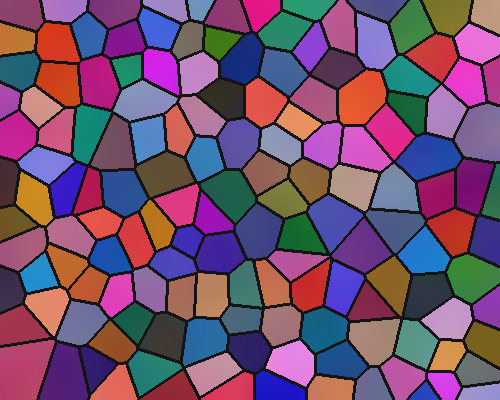
\includegraphics[width=20mm]{assets/drawn/grain-map-wide}};
    \node[anchor=north west,label text,text width=22mm] at (121,-8.4) {EBSD map\\ 1000\,×\,800 px\\ 0.5\,µm per px};
    \node[anchor=north west,label text,text width=42mm] at (98.5,-26.6)
      {colour: $(\varphi_1,\Phi,\varphi_2)\to$ red, green, blue};
    \begin{scope}[shift={(99.5,-48.5)}]
      \draw[udsgreymid,line width=0.5pt] (0,13) -- (0,0) -- (18,0);
      \draw[udsdark,line width=0.9pt] (0,0) -- (1.6,8.2) .. controls (4,10.2) and (12,11.6) .. (15.4,11.2)
        -- (16,8.8);
      \node[circle,fill=udsred,inner sep=0pt,minimum size=1.5mm] at (1.6,8.2) {};
      \node[circle,fill=udsred,inner sep=0pt,minimum size=1.5mm] at (16,8.8) {};
    \end{scope}
    \node[anchor=north west,label text,text width=22mm] at (121,-36.6) {tensile test:\\ yield strength,\\ elongation};
  \end{tikzpicture}
  \note{\textbf{11:30--12:40}\par
    The 25 alloys come from an orthogonal design: five hot-rolling reductions, five annealing
      temperatures and five annealing times, combined so that every pair of levels occurs once.\par
    Each cell is one alloy; the number is its annealing time and the shade its yield strength.\par
    More rolling and lower annealing temperatures give the stronger alloys.\par
    Each alloy has one EBSD map of 1000 by 800 pixels at 0.5 µm per pixel, a field of 500 by 400 µm,
      with the three Euler angles of each pixel stored as red, green and blue.\par
    Each alloy also has one yield strength and one elongation; how many tensile tests stand behind them
      is not stated.\par
    So the dataset is 25 maps and 25 pairs of property values.}
\end{frame}

% ----------------------------------------------------------------- split
\begin{frame}[source={Liao et al.\ (2026), Nat.\ Commun.\ 17, 11232, Results and Methods}]{Alloy split before cropping}
  \begin{tikzpicture}[x=1mm,y=1mm]
    \useasboundingbox (0,0) rectangle (144,-54);
    % stages, left to right
    \foreach \x/\t in {32/{EBSD maps},64/{patches, 100\,×\,100\,px},97/{+ flips, rotations},
        128/{+ degraded copies}}
      \node[anchor=north,label text,align=center] at (\x,0) {\t};
    \node[anchor=north,inner sep=0pt] (m1) at (32,-5.2) {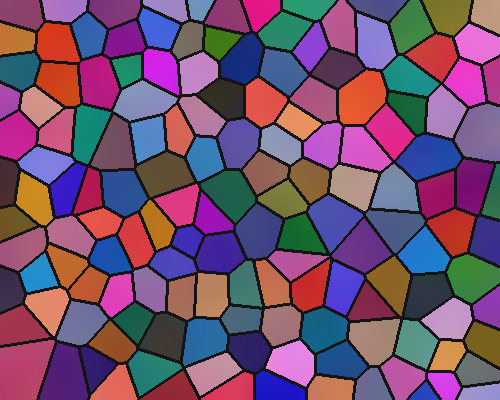
\includegraphics[width=16mm]{assets/drawn/grain-map-wide}};
    \node[anchor=north,inner sep=0pt] (m2) at (64,-5.2) {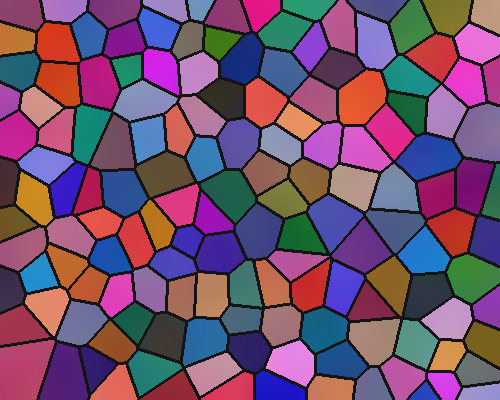
\includegraphics[width=16mm]{assets/drawn/grain-map-wide}};
    \draw[white,line width=0.35pt] \foreach \i in {1,...,9} {([xshift=\i*1.6mm]m2.north west) -- ([xshift=\i*1.6mm]m2.south west)}
      \foreach \j in {1,...,7} {([yshift=-\j*1.6mm]m2.north west) -- ([yshift=-\j*1.6mm]m2.north east)};
    \draw[udsred,line width=0.7pt] (m2.north west) rectangle ([xshift=1.6mm,yshift=-1.6mm]m2.north west);
    \node[inner sep=0pt] at (91.5,-9.7) {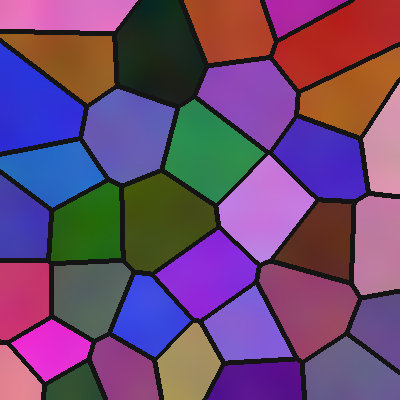
\includegraphics[width=9mm]{assets/drawn/grain-map}};
    \node[inner sep=0pt,rotate=90] at (102.5,-9.7) {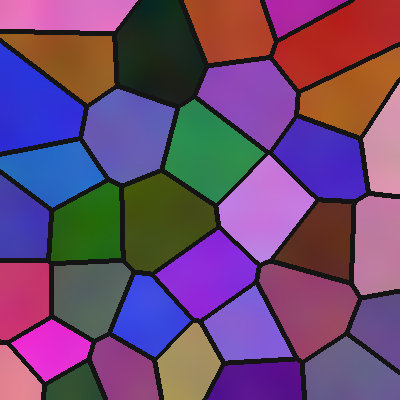
\includegraphics[width=9mm]{assets/drawn/grain-map}};
    \node[inner sep=0pt] at (122.5,-9.7) {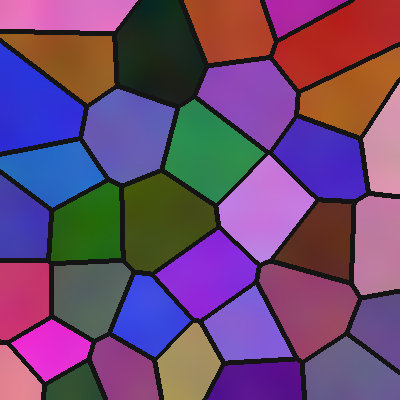
\includegraphics[width=9mm]{assets/drawn/grain-map}};
    \node[inner sep=0pt] at (133.5,-9.7) {
\includegraphics[width=9mm]{assets/drawn/grain-map-blurred}};
    % the two lanes
    \fill[bluetint] (0,-24) rectangle (144,-33.6);
    \fill[redtint] (0,-35.6) rectangle (144,-45.2);
    \node[anchor=west,label text,font=\footnotesize\bfseries,text=udsblue] at (1.6,-28.8) {training};
    \node[anchor=west,label text,font=\footnotesize\bfseries,text=udsred] at (1.6,-40.4) {test};
    \foreach \x/\ta/\tb in {32/{20 alloys}/{5 alloys},64/{1,600}/{400},97/{9,600}/{2,400},128/{57,600}/{14,400}} {
      \node[font=\small\bfseries,text=udsdark,inner sep=0pt] at (\x,-28.8) {\ta};
      \node[font=\small\bfseries,text=udsdark,inner sep=0pt] at (\x,-40.4) {\tb};}
    \foreach \x/\m in {48/\times 80,80.5/\times 6,112.5/\times 6} {
      \draw[flow,draw=udsgreymid] (\x-5,-28.8) -- (\x+5,-28.8);
      \draw[flow,draw=udsgreymid] (\x-5,-40.4) -- (\x+5,-40.4);
      \node[small label,anchor=south] at (\x,-23.4) {$\m$};}
    \goodstrip{-48.4}{test patches come from five alloys the model never sees in training}
  \end{tikzpicture}
  \note{\textbf{12:40--13:30}\par
    The split comes first: the 25 maps are divided at random into 20 training and 5 test alloys.\par
    Only then is each map cut into 80 patches of 100 by 100 pixels, 50 by 50 µm.\par
    Flips and rotations make six versions of each patch.\par
    Each version also gets five degraded copies (blur, distortion, black blocks, erosion and dilation),
      which the model learns to restore.\par
    That gives 72,000 images: 57,600 for training and 14,400 for testing.\par
    Because the split is by alloy, no test patch shares a map with a training patch: the same rule as
      splitting by specimen in segmentation.\par
    The images multiply; the alloys stay 25.}
\end{frame}

% ------------------------------------------------------------- generator
\begin{frame}[source={Liao et al.\ (2026), Nat.\ Commun.\ 17, 11232, Fig.\ 1a (CC BY-NC-ND 4.0) · Pandey et al.\ (2022), Trans.\ Mach.\ Learn.\ Res.}]
  {A VAE, refined by diffusion}
  \begin{tikzpicture}[x=1mm,y=1mm]
    \useasboundingbox (0,0) rectangle (144,-54);
    % Fig. 1a as published: its schematic, without the loss equation below it (pixel rows 0 to 258)
    \figpart{0}{0}{1}{0}{0}{2000}{258}{144}
    % the size of each part, under it; x from the part's pixel columns in the figure
    \tikzset{size/.style={anchor=north,small label,text=udsdark,align=center}}
    \node[size] at ({\fpx{113}},-19.8) {$100\times100$ px};
    \node[size,text=udsred] at ({\fpx{521}},-19.8) {128 numbers};
    \node[size] at ({\fpx{918}},-19.8) {$100\times100$ px};
    \node[size] at ({\fpx{1455}},-19.8) {one U-Net for every step};
    \node[size,anchor=north east] at (144,-19.8) {$100\times100$ px};
    % the two models, each under a bracket
    \draw[udsblue,line width=0.6pt] ({\fpx{40}},-23.6) -- ++(0,-1.4) -| ({\fpx{990}},-23.6);
    \node[anchor=north,label text,align=center,text width=68mm] at ({\fpx{515}},-26.4)
      {\textbf{variational autoencoder (VAE)}\\ three convolutional layers in, three transposed out\\
       loss $L_{\mathrm{pix}}+L_{\mathrm{edge}}+L_{\mathrm{SSIM}}+L_{\mathrm{KL}}$};
    \draw[udsblue,line width=0.6pt] ({\fpx{1148}},-23.6) -- ++(0,-1.4) -| ({\fpx{1997}},-23.6);
    \node[anchor=north,label text,align=center,text width=60mm] at ({\fpx{1572}},-26.4)
      {\textbf{conditional diffusion model (DDPM)}\\ a U-Net predicts the noise, guided by $x_V$\\
       loss: the same three terms on the noise};
    % how the generator is trained, and how it generates
    \foreach \i/\c/\icon/\h/\b in {
        0/udsblue/\faImages/training data/{57,600 images of the 20 training alloys: patches to reproduce,
          and degraded copies to restore},
        1/udsred/\faStar/generation/{a code from the search goes through the decoder, then the diffusion
          model: a new patch}} {
      \fill[\c!8] ({\i*74},-39) rectangle ++(70,-14.6);
      \fill[\c] ({\i*74},-39) rectangle ++(1.2,-14.6);
      \node[anchor=north west,inner sep=0pt,font=\scriptsize\bfseries,text=\c] at ({\i*74+3.4},-40.8)
        {\icon\enspace\h};
      \node[anchor=north west,inner sep=0pt,font=\scriptsize,text=udsdark,text width=64.6mm,align=left,
        execute at begin node={\hyphenpenalty=10000\raggedright}] at ({\i*74+3.4},-44.8) {\b};}
  \end{tikzpicture}
  \note{\textbf{13:30--14:20}\par
    This is the paper's own diagram of its generator, Fig.~1a.\par
    The VAE compresses each patch of 100 by 100 pixels into a code z of 128 numbers and decodes it into
      $x_V$, which is smooth.\par
    A conditional diffusion model then refines $x_V$: its U-Net predicts the noise step by step and sees
      $x_V$ at every step, the pairing of DiffuseVAE; the red arrow marks that condition.\par
    Both models are trained with the pixel, edge and SSIM terms of the next slide: the VAE on its output,
      the diffusion model on the noise it predicts.\par
    Training uses the 57,600 images of the 20 training alloys, with Adam over 100 epochs.\par
    The code z is what the search moves around later.}
\end{frame}

% ------------------------------------------------------------------ loss
\begin{frame}[source={Liao et al.\ (2026), Nat.\ Commun.\ 17, 11232, Eqs.\ 1--9 · Sobel and Feldman (1968), Stanford AI Project · Wang et al.\ (2004), IEEE Trans.\ Image Process.\ 13, 600}]{Optimization Loss}
  \begin{tikzpicture}[x=1mm,y=1mm]
    \useasboundingbox (0,0) rectangle (144,-54);
    % the equation, each term above its column
    \foreach \x/\t in {5/{L\;=},22/{L_{\mathrm{pix}}},47/{+},72/{\color{udsblue}L_{\mathrm{edge}}},97/{+},
        122/{\color{udsblue}L_{\mathrm{SSIM}}}}
      \node[font=\LARGE,text=udsdark,inner sep=0pt] at (\x,-3.2) {$\t$};
    \foreach \x/\c/\h in {0/udsgreymid/{pixel values},50/udsblue/{edges},100/udsblue/{structure}} {
      \fill[\c!8] (\x,-16.6) rectangle ++(44,-35.4);
      \cardhead{\x}{-11.2}{44}{\c}{\h}}
    % pixel values
    \node[anchor=north,font=\small,text=udsdark,inner sep=0pt] at (22,-19.6)
      {$\displaystyle\frac{1}{n}\sum_{i=1}^{n}|x_i-\hat{x}_i|$};
    \node[anchor=north west,card text,text width=40mm] at (2,-31)
      {Mean Absolute\\ Difference (MAE)\\[0.8mm] every pixel weighs the same; boundaries are few pixels};
    % edges
    \node[anchor=north,font=\small,text=udsdark,inner sep=0pt] at (72,-19.6)
      {$\mathrm{mean}\,|S\ast x-S\ast\hat{x}|$};
    \node[anchor=north west,inner sep=0pt] (e1) at (54,-25.4) {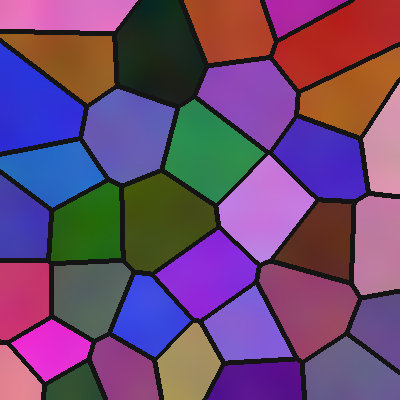
\includegraphics[width=12mm]{assets/drawn/grain-map}};
    \node[anchor=north west,inner sep=0pt] (e2) at (78,-25.4) {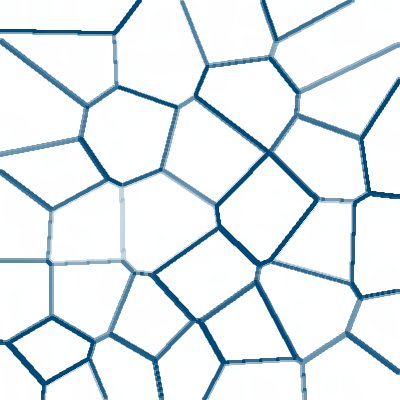
\includegraphics[width=12mm]{assets/drawn/grain-map-edges}};
    \draw[icon frame,udsgreylight] (e2.south west) rectangle (e2.north east);
    \draw[flow,draw=udsblue] (e1.east) -- node[above=0.6mm,small label,text=udsblue] {$S\ast$} (e2.west);
    \node[anchor=north west,card text,text width=40mm] at (52,-40)
      {Sobel filter $S$, across and down: large at grain boundaries};
    % structure
    \node[anchor=north,font=\small,text=udsdark,inner sep=0pt] at (122,-19.6)
      {$1-\mathrm{SSIM}(x,\hat{x})$};
    \node[anchor=north west,inner sep=0pt] (s1) at (104,-25.4) {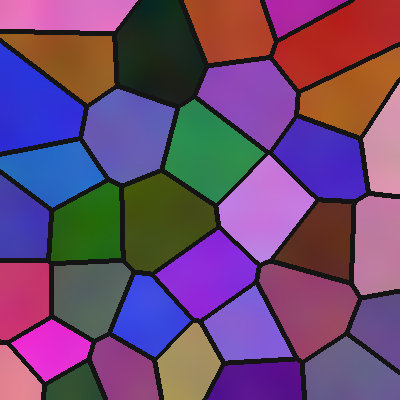
\includegraphics[width=12mm]{assets/drawn/grain-map}};
    \node[anchor=north west,inner sep=0pt] (s2) at (128,-25.4) {
\includegraphics[width=12mm]{assets/drawn/grain-map-blurred}};
    \node[small label,text=udsblue] at (122,-31.4) {$x$ vs $\hat{x}$};
    \node[anchor=north west,card text,text width=40mm] at (102,-40)
      {means, contrasts and correlation: orientation inside grains};
  \end{tikzpicture}
  \note{\textbf{14:20--15:30}\par
    The loss is the sum of three terms, added without weights.\par
    The pixel term is the mean absolute difference between original and reconstruction; boundaries
      cover few pixels, so it hardly sees them.\par
    The edge term applies the Sobel filter, a three-by-three derivative filter from Sobel and Feldman,
      1968, across and down both images and compares the responses: it is large where colours change,
      at grain boundaries.\par
    The structure term is one minus the structural similarity index (SSIM) of Wang and colleagues, 2004,
      which compares the means, contrasts and correlation of the two images; the authors use it for the
      orientation inside and between grains.\par
    The VAE adds its Kullback--Leibler term; the diffusion model applies the same three terms to the
      noise it predicts.\par
    All three compare colours, that is, Euler angles read as intensities.}
\end{frame}

% ------------------------------------------------------------------ SSIM
\begin{frame}[source={Liao et al.\ (2026), Nat.\ Commun.\ 17, 11232, Eqs.\ 4--9 · Wang et al.\ (2004), IEEE Trans.\ Image Process.\ 13, 600}]{Structural Similarity (SSIM)}
  \begin{tikzpicture}[x=1mm,y=1mm]
    \useasboundingbox (0,0) rectangle (144,-54);
    \tikzset{pair image/.style={anchor=north west,inner sep=0pt},
      component value/.style={anchor=north,inner sep=0pt,font=\scriptsize,text=udsdark},
      component formula/.style={anchor=north,inner sep=0pt,font=\footnotesize,text=udsdark},
      component meaning/.style={anchor=north,inner sep=0pt,font=\scriptsize,text=udsdark}}
    % three components; each compares the patch with a copy that changes only what it measures
    \foreach \i/\h in {0/{luminance $L$},1/{contrast $C$},2/{structure $S$}} {
      \fill[bluetint] ({\i*49},-5.4) rectangle ++(46,-29.4);
      \cardhead{\i*49}{0}{46}{udsblue}{\h}
      \node[pair image] at ({\i*49+7.4},-7.4) {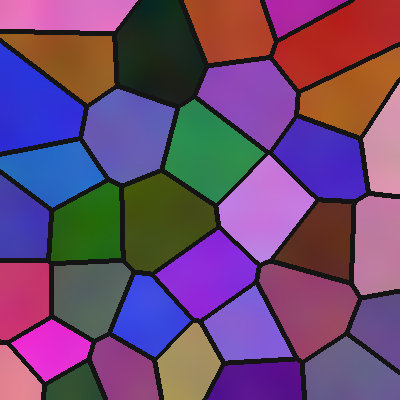
\includegraphics[width=11mm]{assets/drawn/grain-map}};
      \node[small label,text=udsdark] at ({\i*49+23},-12.9) {vs};}
    \node[pair image] at (28.6,-7.4) {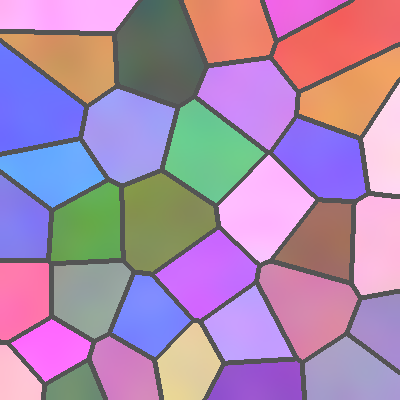
\includegraphics[width=11mm]{assets/drawn/ssim-bright}};
    \node[pair image] at (77.6,-7.4) {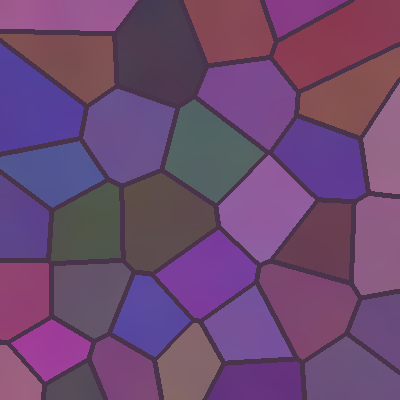
\includegraphics[width=11mm]{assets/drawn/ssim-flat}};
    \node[pair image] at (126.6,-7.4) {
\includegraphics[width=11mm]{assets/drawn/ssim-shuffled}};
    \node[component value] at (23,-19.6)
      {\textcolor{udsred}{$L=\ssimBrightL$}\enspace $C=\ssimBrightC$\enspace $S=\ssimBrightS$};
    \node[component value] at (72,-19.6)
      {$L=\ssimFlatL$\enspace \textcolor{udsred}{$C=\ssimFlatC$}\enspace $S=\ssimFlatS$};
    \node[component value] at (121,-19.6)
      {$L=\ssimShuffledL$\enspace $C=\ssimShuffledC$\enspace \textcolor{udsred}{$S=\ssimShuffledS$}};
    \node[component formula] at (23,-23.2) {$\dfrac{2\mu_x\mu_{\hat x}+C_1}{\mu_x^2+\mu_{\hat x}^2+C_1}$};
    \node[component formula] at (72,-23.2) {$\dfrac{2\sigma_x\sigma_{\hat x}+C_2}{\sigma_x^2+\sigma_{\hat x}^2+C_2}$};
    \node[component formula] at (121,-23.2) {$\dfrac{\sigma_{x\hat x}+C_3}{\sigma_x\sigma_{\hat x}+C_3}$};
    \node[component meaning] at (23,-31) {brightness: the means $\mu$};
    \node[component meaning] at (72,-31) {contrast: the spreads $\sigma$};
    \node[component meaning] at (121,-31) {pattern: the covariance $\sigma_{x\hat x}$};
    % multiplied as the paper does, and turned into a loss
    \fill[bluetint] (0,-37.6) rectangle (144,-53.6);
    \node[anchor=west,inner sep=0pt,font=\footnotesize,text=udsdark] at (2.4,-42.6)
      {$\mathrm{SSIM}=L^{\alpha}\,C^{\beta}\,S^{\gamma}$};
    \node[anchor=west,small label,text=udsdark,text width=44mm] at (2.4,-48.8)
      {paper: $\alpha=\beta=\gamma=1$, $C_3=C_2/2$};
    \node[anchor=west,inner sep=0pt,font=\footnotesize,text=udsdark] (eq8) at (46.6,-45.6)
      {$=\dfrac{(2\mu_x\mu_{\hat x}+C_1)(2\sigma_{x\hat x}+C_2)}{(\mu_x^2+\mu_{\hat x}^2+C_1)(\sigma_x^2+\sigma_{\hat x}^2+C_2)}$};
    \draw[flow,draw=udsblue] ([xshift=1.6mm]eq8.east) -- ++(5.4,0);
    \node[anchor=west,inner sep=0pt,font=\footnotesize,text=udsdark] (loss) at ([xshift=8.6mm]eq8.east)
      {$L_{\mathrm{SSIM}}=1-\mathrm{SSIM}$};
    \node[anchor=north west,small label,text=udsdark] at ([yshift=-1.4mm]loss.south west) {zero for identical patches};
  \end{tikzpicture}
  \note{\textbf{15:30--16:40}\par
    SSIM compares two patches in three ways, each through one statistic of the pixel values.\par
    Luminance compares the means: a brighter copy of the patch scores $L=\ssimBrightL$, while $C$ and $S$
      stay near 1.\par
    Contrast compares the standard deviations: a flattened copy scores $C=\ssimFlatC$.\par
    Structure compares the patterns through the covariance: shuffling the patch's tiles keeps its mean
      and spread but drops $S$ to \ssimShuffledS.\par
    The product, with all exponents 1 and $C_3=C_2/2$ as in the paper, gives its Eq.~8; the loss is one
      minus SSIM.\par
    The brighter copy differs by \ssimBrightM{} per pixel on average and keeps SSIM \ssimBrightQ; the blurred
      patch of slide 4 differs by only \ssimBlurredM{} but drops to \ssimBlurredQ: SSIM sees lost structure
      that a pixel loss barely notices.}
\end{frame}

% --------------------------------------------------- failure case, fixed
\begin{frame}[source={Liao et al.\ (2026), Nat.\ Commun.\ 17, 11232, Fig.\ 2c (CC BY-NC-ND 4.0)}]
  {The same patches, with the new loss}
  \begin{tikzpicture}[x=1mm,y=1mm]
    \useasboundingbox (0,0) rectangle (144,-54);
    \figpart{36}{0}{2}{340}{770}{1897}{1537}{104}
    \node[anchor=east,label text,align=right] at (33,{\fpy{884}}) {real patches};
    \node[anchor=east,label text,align=right,text=udsred] at (33,{\fpy{1155}}) {pixel loss only};
    \node[anchor=east,label text,align=right,text=testgreen] at (33,{\fpy{1423}}) {with edge and\\SSIM terms};
  \end{tikzpicture}
  \note{\textbf{16:40--17:20}\par
    The same six test patches, with a third row: the model trained with all three terms.\par
    The boundaries are sharp again, and each grain has nearly one colour.\par
    The pixel loss itself also falls, from about 0.20 to about 0.10 according to the text; the plotted
      curve settles nearer 0.07.\par
    Two more reconstruction terms also weaken the Kullback--Leibler term relative to the rest, which by
      itself can lower a VAE's reconstruction error; the paper does not separate the two effects.\par
    The comparison with a standard VAE, a Wasserstein GAN and a standard DDPM is only in the
      Supplementary Information.}
\end{frame}

% ------------------------------------------------------------ descriptor
\begin{frame}[source={Liao et al.\ (2026), Nat.\ Commun.\ 17, 11232, after Fig.\ 4a and Methods · Pearson (1901), Philos.\ Mag.\ 2, 559}]{Six numbers per alloy}
  \begin{tikzpicture}[x=1mm,y=1mm]
    \useasboundingbox (0,0) rectangle (144,-54);
    \tikzset{dims/.style={anchor=north,small label,text=udsdark,align=center},
      op/.style={small label,text=udsgrey,align=center},
      back/.style={anchor=north,small label,text=udsred,align=center}}
    % one alloy's map, cut into 10 x 8 patches of 100 x 100 pixels
    \node[anchor=north west,inner sep=0pt] at (0,0) {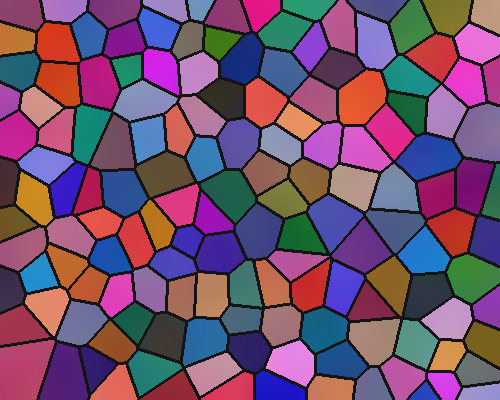
\includegraphics[width=25mm]{assets/drawn/grain-map-wide}};
    \draw[white,line width=0.35pt] \foreach \i in {1,...,9} {(\i*2.5,0) -- (\i*2.5,-20)}
      \foreach \j in {1,...,7} {(0,-\j*2.5) -- (25,-\j*2.5)};
    \node[dims] at (12.5,-20.8) {one alloy, $1000\times800$ px:\\ 80 patches};
    % the encoder gives one code of 128 numbers per patch
    \draw[flow] (25.6,-10) -- (28.2,-10);
    \filldraw[fill=bluetint,draw=udsblue,line width=0.5pt] (28.8,-3.4) -- (36.4,-6.8) -- (36.4,-13.2) -- (28.8,-16.6) -- cycle;
    \node[label text,rotate=90,font=\scriptsize] at (32.4,-10) {encoder};
    \draw[flow] (37,-10) -- (39.6,-10);
    \codematrix{40.2}{-1}{16}{18}{1}
    \node[dims] at (48.2,-20.8) {80 codes\\ $\times$ 128 numbers};
    % mean and spread over the 80 patches
    \draw[flow] (56.8,-7.2) -- node[above=0.4mm,op,sloped] {mean} (65.4,-5.4);
    \draw[flow] (56.8,-12.8) -- node[below=0.4mm,op,sloped] {spread} (65.4,-14.6);
    \pgfmathsetseed{80}
    \foreach \c in {0,...,15} {
      \pgfmathtruncatemacro\shadeA{20+50*rnd}
      \pgfmathtruncatemacro\shadeB{10+45*rnd}
      \filldraw[fill=udsblue!\shadeA,draw=udsblue,line width=0.3pt] ({66+1.25*\c},-4.2) rectangle ++(1.25,-2.4);
      \filldraw[fill=udsdark!\shadeB,draw=udsdark,line width=0.3pt] ({66+1.25*\c},-13.4) rectangle ++(1.25,-2.4);}
    \node[anchor=south,small label,text=udsdark] at (76,-3.6) {$\mu$: 128 numbers};
    \node[dims] at (76,-16.4) {$\sigma$: 128 numbers};
    % PCA, fitted on the 25 alloys: the first three components of each
    \draw[flow] (86.6,-5.4) -- node[above=0.4mm,op] {PCA} (92.4,-5.4);
    \draw[flow] (86.6,-14.6) -- node[below=0.4mm,op] {PCA} (92.4,-14.6);
    \foreach \j in {0,1,2} {
      \filldraw[fill=bluetint,draw=udsblue,line width=0.5pt] ({93+2.4*\j},-4.2) rectangle ++(2.4,-2.4);
      \filldraw[fill=darktint,draw=udsdark,line width=0.5pt] ({93+2.4*\j},-13.4) rectangle ++(2.4,-2.4);}
    \node[op,anchor=north] at (96.6,-19.6) {first 3 of\\ 24 components};
    % the descriptor
    \draw[flow] (100.8,-5.4) to[out=0,in=180] (107.4,-9.4);
    \draw[flow] (100.8,-14.6) to[out=0,in=180] (107.4,-10.6);
    \descstrip{108}{-8.8}{2.4}{2.4}
    \node[anchor=south,small label,text=udsdark] at (115.2,-8.2) {descriptor};
    \node[anchor=west,small label,text=udsdark] at (123.2,-10) {6 numbers};
    % the table it fills: one row per alloy, beside the measured properties
    \draw[flow] (115.2,-11.6) -- (115.2,-31.8);
    \descstrip{108}{-32.4}{2.4}{3}
    \foreach \x/\l in {122.4/YS,129.4/El}
      \node[draw=udsgreymid,fill=darktint,line width=0.3pt,minimum width=7mm,minimum height=3mm,inner sep=0pt,
        anchor=north west,font=\scriptsize,text=udsdark] at (\x,-32.4) {\l};
    \foreach \r in {1,...,3} \foreach \x/\w in {108/14.4,122.4/7,129.4/7}
      \draw[udsgreylight,line width=0.3pt,fill=white] (\x,{-32.4-3*\r}) rectangle ++(\w,-3);
    \node[small label,text=udsdark] at (122.4,-45.4) {$\vdots$};
    \node[dims,text width=36mm] at (122.4,-48.9) {25 alloys: six numbers, yield strength, elongation};
    % the way back, which the search uses: below the labels, up to the map's label at the end
    \draw[udsred,line width=0.6pt,dash pattern=on 1.6pt off 1.2pt,-{Stealth[length=1.6mm,width=1.2mm]}]
      (109.2,-11.6) -- (109.2,-31) -- (12.5,-31) -- (12.5,-27.6);
    \foreach \x/\l in {96.6/inverse PCA,76/{$\mu$, $\sigma$},48.2/draw 80 codes,32.6/decode}
      \node[back] at (\x,-31.8) {\l};
    \node[anchor=north west,small label,text=udsred,text width=92mm] at (0,-36.4)
      {the way back, for the search: six numbers give a mean and a spread, 80 codes are drawn from them and
       decoded into new patches};
  \end{tikzpicture}
  \note{\textbf{17:20--18:10}\par
    To link microstructures with properties, each alloy needs one descriptor.\par
    The 80 patches of its map are encoded, which gives 80 codes of 128 numbers.\par
    Their mean and standard deviation over the patches describe the alloy: what its patches look like
      on average, and how much they vary.\par
    Principal component analysis (PCA, Pearson 1901), fitted on the 25 alloys, keeps the first three of
      24 components of each, so every alloy becomes six numbers beside its measured properties.\par
    PCA can be inverted, the red path: six numbers map back to a mean and a spread, from which new codes
      are drawn and decoded.\par
    The number of components was chosen by the fidelity of the generated patches (Supplementary
      Information).}
\end{frame}

% ---------------------------------------------------------------- search
\begin{frame}[source={Liao et al.\ (2026), Nat.\ Commun.\ 17, 11232, after Fig.\ 4a · Deb et al.\ (2002), IEEE Trans.\ Evol.\ Comput.\ 6, 182}]{A genetic search in six numbers}
  \begin{tikzpicture}[x=1mm,y=1mm]
    \useasboundingbox (0,0) rectangle (144,-54);
    \tikzset{glyph label/.style={anchor=north,small label,text=udsdark,align=center},
      op/.style={anchor=south,small label,text=udsgrey,align=center,yshift=1mm}}
    % the loop: four steps on cards, run for 500 generations
    \foreach \i/\h in {0/population,1/predict,2/keep the best,3/{cross over, mutate}} {
      \pgfmathsetmacro\cx{\i*38}
      \fill[bluetint] (\cx,-5.4) rectangle ++(30,-13.4);
      \cardhead{\cx}{0}{30}{udsblue}{\h}}
    \foreach \i in {0,1,2} \draw[flow,draw=udsblue] ({\i*38+30.4},-12.1) -- ({\i*38+37.6},-12.1);
    % population: 10 descriptors of six numbers
    \foreach \k in {0,...,4} {\descstrip{4}{-7-1.7*\k}{1.5}{1.2}\descstrip{17}{-7-1.7*\k}{1.5}{1.2}}
    \node[glyph label] at (15,-15.6) {10 descriptors};
    % predict: one tree model per property
    \minitree{45.5}{-7.2}
    \minitree{60.5}{-7.2}
    \node[glyph label] at (45.5,-14.2) {strength};
    \node[glyph label] at (60.5,-14.2) {elongation};
    % keep the best: fronts and crowding, as on slide 10
    \begin{scope}[shift={(80.5,-17.4)}]
      \draw[udsgreymid,line width=0.4pt] (0,10.4) -- (0,0) -- (22,0);
      \begin{scope}[x=22mm,y=10mm]
        \drawfronttwo[udsgreymid,line width=0.5pt,dash pattern=on 1.2pt off 0.9pt]
        \drawfrontone[udsblue,line width=0.7pt]
        \foreach \x/\y/\r in \paretopoints {
          \ifcase\r\or\def\rc{udsblue}\or\def\rc{udsgreymid}\else\def\rc{udsgreylight}\fi
          \node[circle,fill=\rc,inner sep=0pt,minimum size=1.2mm] at (\x,\y) {};}
      \end{scope}
    \end{scope}
    % cross over and mutate: a child from two parents, one number changed
    \foreach \j in {0,...,5} {
      \filldraw[fill=udsblue!20,draw=udsblue,line width=0.3pt] ({116.6+1.8*\j},-7.4) rectangle ++(1.8,-1.8);
      \filldraw[fill=udsblue!65,draw=udsblue,line width=0.3pt] ({116.6+1.8*\j},-10.4) rectangle ++(1.8,-1.8);
      \ifnum\j<3\def\cf{udsblue!20}\else\def\cf{udsblue!65}\fi
      \ifnum\j=4\def\cf{udsred!70}\fi
      \filldraw[fill=\cf,draw=udsblue,line width=0.3pt] ({131.4+1.8*\j},-8.9) rectangle ++(1.8,-1.8);}
    \draw[flow,draw=udsblue,line width=0.5pt] (128.4,-9.8) -- (130.8,-9.8);
    \node[glyph label] at (122,-13.4) {parents};
    \node[glyph label] at (136.8,-13.4) {child, one\\ number mutated};
    % 500 generations: the way round
    \draw[flow,draw=udsblue] (129,-18.8) -- (129,-21.8) -- (15,-21.8) -- (15,-19.2);
    \node[fill=white,inner sep=1mm,font=\footnotesize\bfseries,text=udsblue] at (72,-21.8) {500 generations};
    % the way back to microstructures, for the 5 best
    \draw[flow] (5,-18.8) -- (5,-30.8);
    \node[anchor=west,small label,text=udsdark] at (6.4,-25) {the 5 best};
    \foreach \k in {0,...,4} \descstrip{0}{-31.4-1.8*\k}{1.8}{1.3}
    \node[glyph label] at (5.4,-41.6) {5 descriptors};
    \draw[flow] (12.2,-36) -- node[op] {inverse\\ PCA} (26.4,-36);
    \pgfmathsetseed{80}
    \foreach \c in {0,...,15} {
      \pgfmathtruncatemacro\shadeA{20+50*rnd}
      \pgfmathtruncatemacro\shadeB{10+45*rnd}
      \filldraw[fill=udsblue!\shadeA,draw=udsblue,line width=0.3pt] ({27.2+1.25*\c},-32.6) rectangle ++(1.25,-2.4);
      \filldraw[fill=udsdark!\shadeB,draw=udsdark,line width=0.3pt] ({27.2+1.25*\c},-37) rectangle ++(1.25,-2.4);}
    \node[glyph label] at (37.2,-40.2) {$\mu$, $\sigma$: 128 each};
    \draw[flow] (48,-36) -- node[op] {draw\\ 80 codes} (62.2,-36);
    \codematrix{63}{-30.6}{12}{11}{1}
    \node[glyph label] at (69,-42.4) {80 codes};
    \draw[flow] (75.8,-36) -- node[op] {decode,\\ refine} (90,-36);
    \node[anchor=north west,inner sep=0pt] at (90.8,-29.6) {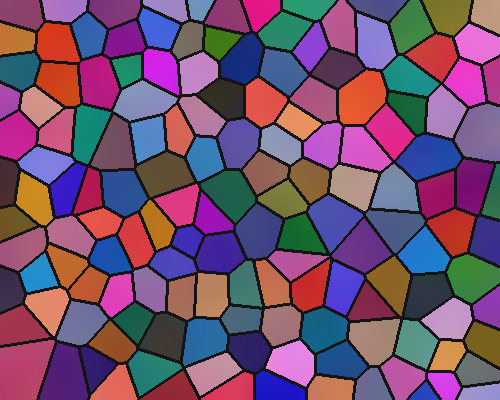
\includegraphics[width=25mm]{assets/drawn/grain-map-wide}};
    \draw[white,line width=0.35pt] \foreach \i in {1,...,9} {(90.8+\i*2.5,-29.6) -- (90.8+\i*2.5,-49.6)}
      \foreach \j in {1,...,7} {(90.8,-29.6-\j*2.5) -- (115.8,-29.6-\j*2.5)};
    \node[glyph label] at (103.3,-50.2) {80 new patches};
    \node[text=udsred,font=\small] at (120.2,-34.4) {\faStar};
    \node[anchor=north west,label text,text width=21mm,text=udsred] at (122.6,-32.4)
      {a proposed microstructure for each descriptor};
  \end{tikzpicture}
  \note{\textbf{18:10--19:00}\par
    The loop of section 2, run on the six numbers.\par
    Two gradient-boosted tree models, one per property, fitted on the 20 training alloys, predict yield
      strength and elongation from a descriptor; they are the objectives.\par
    NSGA-II evolves a population of 10 descriptors over 500 generations; the paper's average hypervolume
      improvement, the area the candidates span above the weakest measured alloy, levels off after about
      150 generations.\par
    The five best final descriptors go back through the inverse PCA to a mean and a spread; 80 codes are
      drawn from them and decoded into patches, the proposed microstructures.}
\end{frame}

\section[Results]{The results}
\sectionframe{04}{The results}{What do the authors show?}{\faChartBar}

% ------------------------------------------------------------ fidelity
\begin{frame}[source={Liao et al.\ (2026), Nat.\ Commun.\ 17, 11232, Fig.\ 3i--n (CC BY-NC-ND 4.0)}]
  {Grain statistics after reconstruction}
  \begin{tikzpicture}[x=1mm,y=1mm]
    \useasboundingbox (0,0) rectangle (144,-54);
    \figpart{0}{0}{3}{0}{700}{2000}{1883}{91}
    % the two rows of panels, by the figure's own panel letters
    \node[anchor=north west,label text,text width=46mm] at (98,-0.6) {original against reconstruction};
    \node[anchor=west,label text,text width=46mm] at (98,-8.4) {\textbf{i--k}\enspace grain area and ellipse axes};
    \node[anchor=west,label text,text width=46mm] at (98,-13.8) {\textbf{l--n}\enspace the three Euler angles};
    \node[circle,fill=udsgreylight,inner sep=0pt,minimum size=2mm] at (99.4,-20.6) {};
    \node[anchor=west,label text,text width=41mm] at (102,-20.6) {2,000 single patches: wide scatter};
    \node[circle,fill=udsblue!75,inner sep=0pt,minimum size=2mm] at (99.4,-27.4) {};
    \node[anchor=west,label text,text width=41mm] at (102,-27.4) {20 training alloys, each the mean of 80 patches};
    \node[rectangle,fill=udsred!80,inner sep=0pt,minimum size=2mm] at (99.4,-34.2) {};
    \node[anchor=west,label text,text width=41mm] at (102,-34.2) {5 test alloys};
    \draw[udsred,line width=0.6pt,dash pattern=on 1.4pt off 1pt] (98,-39.6) -- (100.8,-39.6);
    \node[anchor=west,label text] at (102,-39.6) {reconstruction = original};
  \end{tikzpicture}
  \note{\textbf{19:10--20:00}\par
    Six features are measured in each original patch and its reconstruction: grain area, the major
      and minor axes of the equivalent ellipse (panels i to k), and the three Euler angles (l to n).\par
    The grey points are the 2,000 single patches; their means scatter widely, more so for large grains,
      of which one patch holds only a few.\par
    Averaged over the 80 patches of each alloy, the 20 training alloys in blue and the 5 test alloys in
      red lie on the line of equality.\par
    So the model reproduces the grain statistics of alloys it never saw.\par
    What is compared: reconstructions with their own inputs, the first task of slide 7.\par
    Misorientation statistics and the baseline models are in the Supplementary Information only.}
\end{frame}

% ---------------------------------------------------------- surrogates
\begin{frame}[source={Liao et al.\ (2026), Nat.\ Commun.\ 17, 11232, Fig.\ 4b, c (CC BY-NC-ND 4.0) · Friedman (2001), Ann.\ Stat.\ 29, 1189}]
  {Property predictions}
  \begin{tikzpicture}[x=1mm,y=1mm]
    \useasboundingbox (0,0) rectangle (144,-54);
    \figpart{6}{0}{4}{0}{480}{640}{975}{62}
    \figpart{78}{0}{4}{640}{480}{1260}{975}{60.1}
    \node[anchor=north west,label text,text width=144mm] at (6,-50)
      {Gradient-Boosted Trees on the six numbers: fitted on 20 alloys, tested on 5};
  \end{tikzpicture}
  \note{\textbf{20:00--20:40}\par
    These are two gradient-boosted tree models (Friedman, 2001), one per property: sums of many small
      regression trees on an alloy's six numbers; the number of trees and their depth were set by a
      randomized search.\par
    On the five test alloys, R² is 0.96 for yield strength and 0.92 for elongation; on the 20 training
      alloys 0.96 and 0.93.\par
    R² is the share of the variance of the measured values that the predictions explain.\par
    These two models are what the search optimizes.}
\end{frame}

% ---------------------------------------------------------- candidates
\begin{frame}[source={Liao et al.\ (2026), Nat.\ Commun.\ 17, 11232, after Fig.\ 4f; Fig.\ 4e (CC BY-NC-ND 4.0)}]
  {Five candidates beyond the front}
  \begin{tikzpicture}[x=1mm,y=1mm]
    \useasboundingbox (0,0) rectangle (144,-54);
    \begin{scope}[shift={(14,-41)}]
      \planeaxes{340}{1000}{28}{86}{76}{41}{400,500,...,1000}{30,40,...,80}
      \begin{scope}[plane]
        \drawfront[front]
        \drawalloys
        \drawcandidates
        \node[anchor=west,inner sep=0pt] at ([xshift=1.4mm]cand1.east) {\candlabel{1}};
        \node[anchor=west,inner sep=0pt] at ([xshift=1.4mm]cand2.east) {\candlabel{2}};
      \end{scope}
      \node[alloy] at (52,39.4) {};
      \node[anchor=west,small label,text=udsdark] at (54,39.4) {measured};
      \node[candidate] at (52,35.4) {};
      \node[anchor=west,small label,text=udsdark] at (54,35.4) {candidates};
    \end{scope}
    \node[axis label] at (52,-48.4) {yield strength (MPa)};
    \node[axis label,rotate=90] at (3,-20.5) {elongation (\%)};
    % the latent plane of Fig. 4e
    \figpart{95}{0}{4}{1280}{480}{2000}{975}{49}
    \node[anchor=north west,small label,text width=49mm] at (95,-35.6)
      {first principal components of mean and spread: generated (red) beside measured (grey)};
  \end{tikzpicture}
  \note{\textbf{20:40--21:40}\par
    After 500 generations the search returns five candidates, here with their predicted properties.\par
    All five lie above the measured front: at equal strength, they are predicted to stretch more.\par
    Their predicted values stay inside the ranges of the 25 measured alloys; the gain lies in their
      combination.\par
    On the right, the first principal components of the mean and the spread: measured alloys in grey,
      generated microstructures as triangles, darker for a larger hypervolume improvement.\par
    The best candidates lie far from every measured alloy; the authors call them out of distribution,
      the third task of slide 7.\par
    Candidates 1 and 2 are the ones checked by simulation.}
\end{frame}

% --------------------------------------------------------- fine grains
\begin{frame}[source={Liao et al.\ (2026), Nat.\ Commun.\ 17, 11232, Fig.\ 5a--d (CC BY-NC-ND 4.0) · Ma and Zhu (2017), Mater.\ Today 20, 323}]
  {Fine grains in the generated patches}
  \begin{tikzpicture}[x=1mm,y=1mm]
    \useasboundingbox (0,0) rectangle (144,-54);
    \figpart{0}{0}{5}{0}{0}{1300}{965}{72}
    % generated patches and their histogram, by the figure's own panel letters
    \node[anchor=west,label text,text width=60mm] at (80,-2.6) {\textbf{b}\enspace fine-grain regions, marked by arrows};
    \node[anchor=west,label text,text width=60mm] at (80,-8) {\textbf{d}\enspace more grains in the smallest bin};
    % the proposed mechanism, on an illustrative map
    \node[anchor=north west,small label] at (80,-13.6) {proposed mechanism};
    \node[anchor=north west,inner sep=0pt] (bm) at (80,-17.4) {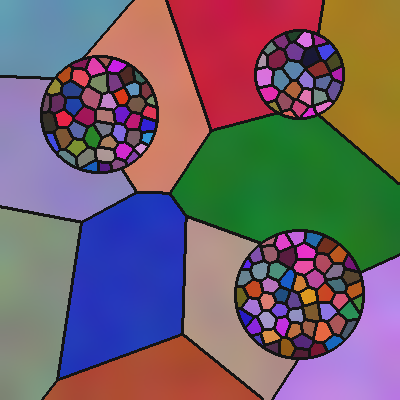
\includegraphics[width=20mm]{assets/drawn/grain-map-bimodal}};
    \node[anchor=west,label text] (fine) at (104,-21.4) {fine grains};
    \draw[udsdark,line width=0.4pt] (fine.west) -- ++(-1.6,0) -- (95,-21.15);
    \node[anchor=west,label text] (coarse) at (104,-28.4) {coarse grains};
    \draw[udsdark,line width=0.4pt] (coarse.west) -- ++(-1.6,0) -- (98,-26.9);
    \node[anchor=north west,card text,text width=63mm] at (80,-39.6)
      {\cardbullet{fine grains block dislocations: strength}
       \cardbullet{coarse grains let them glide: ductility}
       \cardbullet{the mismatch stores dislocations: hardening}};
  \end{tikzpicture}
  \note{\textbf{21:40--22:40}\par
    Left, patches of the initial alloys and patches generated for the candidates; the arrows mark what
      the authors call fine-grain regions (panel b).\par
    Below, the grain areas of all 2,000 original patches and of 400 generated ones, on a logarithmic
      axis: the generated patches have more grains in the smallest bin, at or below 0.4 µm² (panel d),
      which the authors read as a bimodal grain size.\par
    Their explanation: fine grains block dislocations and raise the strength, coarse grains leave room
      for them to glide and keep the ductility, and the mismatch between the two stores geometrically
      necessary dislocations (GNDs), which raise the strain hardening.\par
    The mechanism is established for heterogeneous microstructures; whether these generated patches
      show it remains to be checked.}
\end{frame}

% ------------------------------------------------------------ validation
\begin{frame}[source={Liao et al.\ (2026), Nat.\ Commun.\ 17, 11232, Fig.\ 5e, h (CC BY-NC-ND 4.0)}]
  {Simulation and one experiment}
  \begin{tikzpicture}[x=1mm,y=1mm]
    \useasboundingbox (0,0) rectangle (144,-54);
    \figpart{0}{0}{5}{1430}{49}{1908}{434}{54}
    \node[anchor=north west,label text,text width=54mm] at (0,-46.6)
      {new alloy, route from the literature: 60\,\% rolling at 1000\,°C, 5\,min at 850\,°C};
    \figpart{60}{0}{5}{660}{972}{2000}{1473}{84}
    \node[anchor=north west,label text,text width=84mm] at (60,-33.6)
      {candidate \candlabel{1}: i predicted, ii simulated by crystal plasticity (CPFE), iii measured on
       the new alloy};
  \end{tikzpicture}
  \note{\textbf{22:40--23:40}\par
    Two checks follow.\par
    First, crystal plasticity finite element (CPFE) simulations of two generated patches per candidate,
      with a slip model calibrated on three measured stress--strain curves; the Euler angles come from
      the pixel colours, the dislocation density from a learned mapping.\par
    Second, one experiment: an alloy processed by a route the authors chose from the literature to get
      a bimodal grain size, 60 percent hot rolling at 1000 °C and 5 minutes at 850 °C.\par
    Its EBSD map, left, shows coarse grains among many fine ones.\par
    Right, candidate 1 as predicted, simulated and measured: yield strength about 820, 805 and 825 MPa,
      elongation about 48, 44.5 and 43.5 percent, read from the bars.\par
    The paper concludes that the design is validated.}
\end{frame}

% --------------------------------------------------------------- thank you
% the thanks where the title slide has its title; drawn inside the frame, so that the notes' thumbnail
% shows it too
\begin{frame}[plain,noframenumbering]
\vbox to 0pt{\vskip-2mm\hbox to 0pt{\hskip-8mm\begin{tikzpicture}[x=1mm,y=1mm]
  \useasboundingbox (0,0) rectangle (160,-90);
  \node[anchor=north west,inner sep=0pt] at (8,-8) {\includegraphics[width=30mm]{\udslogo}};
  \node[anchor=north west,inner sep=0pt,text width=88mm,align=left] at (8,-36) {%
    {\fontsize{32}{36}\selectfont\bfseries\color{udsblue}Thank you\par}\vskip4mm
    \textcolor{udsred}{\rule{14mm}{0.8pt}}\par\vskip3mm
    {\fontsize{11}{13}\selectfont\color{udsdark}\insertauthor\par}};
\end{tikzpicture}\hss}\vss}
\par\rule{0pt}{80mm}
\note{\textbf{23:40--24:00}\par
    Thank you.\par
    Questions to open the discussion: would edge and SSIM terms help our segmentation of grain
      boundaries; what minimum grain size do we use in EBSD analysis, and why; how many independent
      specimens would we want before trusting a property model; and what would convince us that a
      generated microstructure is new and can be made.\par
    Backup slides follow: the loss terms in full, the 25 processing routes and the references.}
\end{frame}

\appendix
% the footer numbers appendix slides A1, A2, ..., as their titles do
\setcounter{framenumber}{0}
\renewcommand\insertframenumber{A\arabic{framenumber}}
% Appendix: its own sections, so the mini-frame headline shows only these.
\section[Backup]{Backup}

% ------------------------------------------------------------ loss terms
\begin{frame}[source={Liao et al.\ (2026), Nat.\ Commun.\ 17, 11232, Eqs.\ 2--15}]{A1\enspace The loss terms in full}
  \begin{columns}[T,onlytextwidth]
    \begin{column}{0.48\textwidth}
      \small
      {\scriptsize\color{udsgrey}Sobel kernels and edge term (Eqs.\ 2, 3)}
      \[ S_x=\left[\begin{array}{rrr}-1&0&1\\-2&0&2\\-1&0&1\end{array}\right],\;\;
         S_y=\left[\begin{array}{rrr}-1&-2&-1\\0&0&0\\1&2&1\end{array}\right] \]
      \[ L_{\mathrm{edge}}=\mathrm{mean}\big(|S_x\ast x-S_x\ast\hat{x}|+|S_y\ast x-S_y\ast\hat{x}|\big) \]
      {\scriptsize\color{udsgrey}structural similarity (Eqs.\ 8, 9)}
      \[ \mathrm{SSIM}(x,\hat{x})=\frac{(2\mu_x\mu_{\hat{x}}+C_1)(2\sigma_{x\hat{x}}+C_2)}
         {(\mu_x^2+\mu_{\hat{x}}^2+C_1)(\sigma_x^2+\sigma_{\hat{x}}^2+C_2)} \]
      \[ L_{\mathrm{SSIM}}=1-\mathrm{SSIM}(x,\hat{x}) \]
    \end{column}
    \begin{column}{0.48\textwidth}
      \small
      {\scriptsize\color{udsgrey}VAE, with $x_V$ the reconstruction of $x$ (Eq.\ 11)}
      \[ L_{\mathrm{VAE}}=L_{\mathrm{pix}}+L_{\mathrm{edge}}+L_{\mathrm{SSIM}}+L_{\mathrm{KL}}\big(q(z|x),p(z)\big) \]
      {\scriptsize\color{udsgrey}diffusion: forward process (Eq.\ 13)}
      \[ q(x_t|x)=\mathcal{N}\big(x_t;\sqrt{\bar{\alpha}_t}\,x,(1-\bar{\alpha}_t)\mathbf{I}\big) \]
      {\scriptsize\color{udsgrey}diffusion: loss on the predicted noise $\epsilon_\theta(x_t,t,x_V)$ (Eq.\ 15)}
      \[ L_{\mathrm{DDPM}}=L_{\mathrm{pix}}(\epsilon_\theta,\tilde{\epsilon})+L_{\mathrm{SSIM}}(\epsilon_\theta,\tilde{\epsilon})
         +L_{\mathrm{edge}}(\epsilon_\theta,\tilde{\epsilon}) \]
    \end{column}
  \end{columns}
  \note{\textbf{If asked}\par
    The pixel, edge and SSIM terms are added without weights, in the VAE and in the diffusion model.\par
    In the diffusion model they compare the predicted with the true noise, so their link to grain
      boundaries is indirect.\par
    Eq.\ 14 as printed gives the predicted noise as the mean of the reverse step; standard DDPM sampling
      derives that mean from the predicted noise.\par
    SSIM uses its three factors (luminance, contrast, structure) with equal exponents of one, which
      gives Eq.\ 8; $C_1$ and $C_2$ are small constants.}
\end{frame}

% ----------------------------------------------------------------- the data
\begin{frame}[source={Liao et al.\ (2026), Nat.\ Commun.\ 17, 11232}]{A2\enspace The 25 processing routes}
  \scriptsize\renewcommand\arraystretch{1.08}\setlength\tabcolsep{6pt}
  \def\alloyhead{\toprule
      & \multicolumn{2}{c}{annealing} & rolling & \multicolumn{2}{c}{measured}\\
    ID & °C & h & \% & MPa & \%\\
    \midrule}
  \hfill
  \begin{tabular}[t]{@{}rrrrrr@{}}
    \alloyhead
    \alloytableA
    \bottomrule
  \end{tabular}\hfill\hfill
  \begin{tabular}[t]{@{}rrrrrr@{}}
    \alloyhead
    \alloytableB
    \bottomrule
  \end{tabular}\hfill\null
  \note{\textbf{If asked}\par
    The table of the code repository: each variant's processing route, hot rolling at 900 °C and then
      annealing, with its measured yield strength and elongation.\par
    Every pair of levels occurs once: an orthogonal design.\par
    Alloy 10 is the measured alloy closest in strength to candidate 1.\par
    The paper's 20/5 split is random and not listed; from Fig.\ 4b, the test alloys lie near 375, 445,
      470, 795 and 845 MPa.}
\end{frame}

\section[References]{References}

\begin{frame}{A3\enspace References}
  \begin{columns}[T,onlytextwidth]
  \begin{column}{0.53\textwidth}
  \scriptsize\setlength\parskip{0.6mm}\raggedright
  \textbf{The paper and its code}\par
  W.~Liao, K.~Li, B.~Tang, J.~Fan, J.~Wang, X.~Xue, J.~Li, R.~Yuan (2026). \emph{Generative design of high-fidelity
  microstructures using physics-aware machine learning}. Nature Communications 17, 11232.
  \url{https://doi.org/10.1038/s41467-026-78118-3}, CC~BY-NC-ND~4.0.\par
  W.~Liao, R.~Yuan (2026). \emph{microstructures\_design}, code, trained models and \fn{dataset.csv}, commit 25f6017,
  MIT licence, read 4~Nov~2026.\\ \url{https://github.com/nwpuai4msegroup/microstructures_design};\\ archived at
  \url{https://doi.org/10.5281/zenodo.21897025}.\par
  \textbf{Materials background}\par
  E.~Ma, T.~Zhu (2017). \emph{Towards strength--ductility synergy through the design of heterogeneous nanostructures
  in metals}. Materials Today 20(6), 323--331.\par
  \end{column}
  \begin{column}{0.43\textwidth}
  \scriptsize\setlength\parskip{0.4mm}\raggedright
  \textbf{Generative models}\par
  D.~P.~Kingma, M.~Welling (2013). \emph{Auto-encoding variational Bayes}. arXiv:1312.6114; ICLR 2014.\par
  I.~Goodfellow et al.\ (2014). \emph{Generative adversarial nets}. NeurIPS~27.\par
  J.~Sohl-Dickstein, E.~Weiss, N.~Maheswaranathan, S.~Ganguli (2015). \emph{Deep unsupervised learning using
  nonequilibrium thermodynamics}. ICML 2015, PMLR 37, 2256--2265.\par
  J.~Ho, A.~Jain, P.~Abbeel (2020). \emph{Denoising diffusion probabilistic models}. NeurIPS~33.\par
  A.~Ramesh et al.\ (2021). \emph{Zero-shot text-to-image generation}. ICML 2021, PMLR 139, 8821--8831.\par
  R.~Rombach, A.~Blattmann, D.~Lorenz, P.~Esser, B.~Ommer (2022). \emph{High-resolution image synthesis with latent
  diffusion models}. CVPR 2022, 10684--10695.\par
  K.~Pandey, A.~Mukherjee, P.~Rai, A.~Kumar (2022). \emph{DiffuseVAE: efficient, controllable and high-fidelity
  generation from low-dimensional latents}. Transactions on Machine Learning Research.\par
  \end{column}
  \end{columns}
\end{frame}

\begin{frame}{A4\enspace References}
  \begin{columns}[T,onlytextwidth]
  \begin{column}{0.48\textwidth}
  \scriptsize\setlength\parskip{0.6mm}\raggedright
  \textbf{Image processing}\par
  I.~Sobel, G.~Feldman (1968). \emph{A 3\,×\,3 isotropic gradient operator for image processing}. Talk at the Stanford
  Artificial Intelligence Project.\par
  Z.~Wang, A.~C.~Bovik, H.~R.~Sheikh, E.~P.~Simoncelli (2004). \emph{Image quality assessment: from error visibility
  to structural similarity}. IEEE Transactions on Image Processing 13(4), 600--612.\par
  O.~Ronneberger, P.~Fischer, T.~Brox (2015). \emph{U-Net: convolutional networks for biomedical image
  segmentation}. MICCAI 2015, 234--241.\par
  \textbf{Optimization}\par
  V.~Pareto (1906). \emph{Manuale di economia politica}. Società Editrice Libraria, Milan.\par
  J.~H.~Holland (1975). \emph{Adaptation in Natural and Artificial Systems}. University of Michigan Press.\par
  K.~Deb, A.~Pratap, S.~Agarwal, T.~Meyarivan (2002). \emph{A fast and elitist multiobjective genetic algorithm:
  NSGA-II}. IEEE Transactions on Evolutionary Computation 6(2), 182--197.\par
  \end{column}
  \begin{column}{0.48\textwidth}
  \scriptsize\setlength\parskip{0.6mm}\raggedright
  \textbf{Statistics}\par
  K.~Pearson (1901). \emph{On lines and planes of closest fit to systems of points in space}. Philosophical
  Magazine 2(11), 559--572.\par
  L.~Breiman, J.~H.~Friedman, R.~A.~Olshen, C.~J.~Stone (1984). \emph{Classification and Regression Trees}.
  Wadsworth.\par
  J.~H.~Friedman (2001). \emph{Greedy function approximation: a gradient boosting machine}. Annals of Statistics
  29(5), 1189--1232.\par
  \end{column}
  \end{columns}
\end{frame}

\end{document}
